\documentclass[]{book}
\usepackage{lmodern}
\usepackage{amssymb,amsmath}
\usepackage{ifxetex,ifluatex}
\usepackage{fixltx2e} % provides \textsubscript
\ifnum 0\ifxetex 1\fi\ifluatex 1\fi=0 % if pdftex
  \usepackage[T1]{fontenc}
  \usepackage[utf8]{inputenc}
\else % if luatex or xelatex
  \ifxetex
    \usepackage{mathspec}
  \else
    \usepackage{fontspec}
  \fi
  \defaultfontfeatures{Ligatures=TeX,Scale=MatchLowercase}
\fi
% use upquote if available, for straight quotes in verbatim environments
\IfFileExists{upquote.sty}{\usepackage{upquote}}{}
% use microtype if available
\IfFileExists{microtype.sty}{%
\usepackage{microtype}
\UseMicrotypeSet[protrusion]{basicmath} % disable protrusion for tt fonts
}{}
\usepackage[margin=1in]{geometry}
\usepackage{hyperref}
\hypersetup{unicode=true,
            pdftitle={Using R for Introduction to Econometrics},
            pdfauthor={Christoph Hanck, Martin Arnold, Alexander Gerber and Martin Schmelzer},
            pdfborder={0 0 0},
            breaklinks=true}
\urlstyle{same}  % don't use monospace font for urls
\usepackage{natbib}
\bibliographystyle{apalike}
\usepackage{color}
\usepackage{fancyvrb}
\newcommand{\VerbBar}{|}
\newcommand{\VERB}{\Verb[commandchars=\\\{\}]}
\DefineVerbatimEnvironment{Highlighting}{Verbatim}{commandchars=\\\{\}}
% Add ',fontsize=\small' for more characters per line
\usepackage{framed}
\definecolor{shadecolor}{RGB}{248,248,248}
\newenvironment{Shaded}{\begin{snugshade}}{\end{snugshade}}
\newcommand{\KeywordTok}[1]{\textcolor[rgb]{0.13,0.29,0.53}{\textbf{#1}}}
\newcommand{\DataTypeTok}[1]{\textcolor[rgb]{0.13,0.29,0.53}{#1}}
\newcommand{\DecValTok}[1]{\textcolor[rgb]{0.00,0.00,0.81}{#1}}
\newcommand{\BaseNTok}[1]{\textcolor[rgb]{0.00,0.00,0.81}{#1}}
\newcommand{\FloatTok}[1]{\textcolor[rgb]{0.00,0.00,0.81}{#1}}
\newcommand{\ConstantTok}[1]{\textcolor[rgb]{0.00,0.00,0.00}{#1}}
\newcommand{\CharTok}[1]{\textcolor[rgb]{0.31,0.60,0.02}{#1}}
\newcommand{\SpecialCharTok}[1]{\textcolor[rgb]{0.00,0.00,0.00}{#1}}
\newcommand{\StringTok}[1]{\textcolor[rgb]{0.31,0.60,0.02}{#1}}
\newcommand{\VerbatimStringTok}[1]{\textcolor[rgb]{0.31,0.60,0.02}{#1}}
\newcommand{\SpecialStringTok}[1]{\textcolor[rgb]{0.31,0.60,0.02}{#1}}
\newcommand{\ImportTok}[1]{#1}
\newcommand{\CommentTok}[1]{\textcolor[rgb]{0.56,0.35,0.01}{\textit{#1}}}
\newcommand{\DocumentationTok}[1]{\textcolor[rgb]{0.56,0.35,0.01}{\textbf{\textit{#1}}}}
\newcommand{\AnnotationTok}[1]{\textcolor[rgb]{0.56,0.35,0.01}{\textbf{\textit{#1}}}}
\newcommand{\CommentVarTok}[1]{\textcolor[rgb]{0.56,0.35,0.01}{\textbf{\textit{#1}}}}
\newcommand{\OtherTok}[1]{\textcolor[rgb]{0.56,0.35,0.01}{#1}}
\newcommand{\FunctionTok}[1]{\textcolor[rgb]{0.00,0.00,0.00}{#1}}
\newcommand{\VariableTok}[1]{\textcolor[rgb]{0.00,0.00,0.00}{#1}}
\newcommand{\ControlFlowTok}[1]{\textcolor[rgb]{0.13,0.29,0.53}{\textbf{#1}}}
\newcommand{\OperatorTok}[1]{\textcolor[rgb]{0.81,0.36,0.00}{\textbf{#1}}}
\newcommand{\BuiltInTok}[1]{#1}
\newcommand{\ExtensionTok}[1]{#1}
\newcommand{\PreprocessorTok}[1]{\textcolor[rgb]{0.56,0.35,0.01}{\textit{#1}}}
\newcommand{\AttributeTok}[1]{\textcolor[rgb]{0.77,0.63,0.00}{#1}}
\newcommand{\RegionMarkerTok}[1]{#1}
\newcommand{\InformationTok}[1]{\textcolor[rgb]{0.56,0.35,0.01}{\textbf{\textit{#1}}}}
\newcommand{\WarningTok}[1]{\textcolor[rgb]{0.56,0.35,0.01}{\textbf{\textit{#1}}}}
\newcommand{\AlertTok}[1]{\textcolor[rgb]{0.94,0.16,0.16}{#1}}
\newcommand{\ErrorTok}[1]{\textcolor[rgb]{0.64,0.00,0.00}{\textbf{#1}}}
\newcommand{\NormalTok}[1]{#1}
\usepackage{longtable,booktabs}
\usepackage{graphicx,grffile}
\makeatletter
\def\maxwidth{\ifdim\Gin@nat@width>\linewidth\linewidth\else\Gin@nat@width\fi}
\def\maxheight{\ifdim\Gin@nat@height>\textheight\textheight\else\Gin@nat@height\fi}
\makeatother
% Scale images if necessary, so that they will not overflow the page
% margins by default, and it is still possible to overwrite the defaults
% using explicit options in \includegraphics[width, height, ...]{}
\setkeys{Gin}{width=\maxwidth,height=\maxheight,keepaspectratio}
\IfFileExists{parskip.sty}{%
\usepackage{parskip}
}{% else
\setlength{\parindent}{0pt}
\setlength{\parskip}{6pt plus 2pt minus 1pt}
}
\setlength{\emergencystretch}{3em}  % prevent overfull lines
\providecommand{\tightlist}{%
  \setlength{\itemsep}{0pt}\setlength{\parskip}{0pt}}
\setcounter{secnumdepth}{5}
% Redefines (sub)paragraphs to behave more like sections
\ifx\paragraph\undefined\else
\let\oldparagraph\paragraph
\renewcommand{\paragraph}[1]{\oldparagraph{#1}\mbox{}}
\fi
\ifx\subparagraph\undefined\else
\let\oldsubparagraph\subparagraph
\renewcommand{\subparagraph}[1]{\oldsubparagraph{#1}\mbox{}}
\fi

%%% Use protect on footnotes to avoid problems with footnotes in titles
\let\rmarkdownfootnote\footnote%
\def\footnote{\protect\rmarkdownfootnote}

%%% Change title format to be more compact
\usepackage{titling}

% Create subtitle command for use in maketitle
\newcommand{\subtitle}[1]{
  \posttitle{
    \begin{center}\large#1\end{center}
    }
}

\setlength{\droptitle}{-2em}
  \title{Using R for Introduction to Econometrics}
  \pretitle{\vspace{\droptitle}\centering\huge}
  \posttitle{\par}
  \author{Christoph Hanck, Martin Arnold, Alexander Gerber and Martin Schmelzer}
  \preauthor{\centering\large\emph}
  \postauthor{\par}
  \predate{\centering\large\emph}
  \postdate{\par}
  \date{2017-11-17}

\usepackage{booktabs}
\usepackage{amsthm}
\makeatletter
\def\thm@space@setup{%
  \thm@preskip=8pt plus 2pt minus 4pt
  \thm@postskip=\thm@preskip
}
\makeatother

\newenvironment{rmdknit}
    {\begin{center}
    \begin{tabular}{|p{0.9\textwidth}|}
    \hline\\
    }
    { 
    \\\\\hline
    \end{tabular} 
    \end{center}
    }

\newenvironment{rmdnote}
    {\begin{center}
    \begin{tabular}{|p{0.9\textwidth}|}
    \hline\\
    }
    { 
    \\\\\hline
    \end{tabular} 
    \end{center}
    }

\usepackage{amsthm}
\newtheorem{theorem}{Theorem}[chapter]
\newtheorem{lemma}{Lemma}[chapter]
\theoremstyle{definition}
\newtheorem{definition}{Definition}[chapter]
\newtheorem{corollary}{Corollary}[chapter]
\newtheorem{proposition}{Proposition}[chapter]
\theoremstyle{definition}
\newtheorem{example}{Example}[chapter]
\theoremstyle{definition}
\newtheorem{exercise}{Exercise}[chapter]
\theoremstyle{remark}
\newtheorem*{remark}{Remark}
\newtheorem*{solution}{Solution}
\let\BeginKnitrBlock\begin \let\EndKnitrBlock\end
\begin{document}
\maketitle

{
\setcounter{tocdepth}{1}
\tableofcontents
}
\chapter{Preface}\label{preface}

\subsubsection*{What this book is (and what it is
not)}\label{what-this-book-is-and-what-it-is-not}
\addcontentsline{toc}{subsubsection}{What this book is (and what it is
not)}

This book is an interactive script aiming to provide students of
economic sciences with a platform-independent E-learning arrangement
that seamlessly intertwines both, teaching of theoretical core knowledge
and empirical skills in undergraduate econometrics. Thereby, the focus
clearly lays on empirical applications with the freely available
statistical software package R and omitts tedious derivations and formal
proof. The script is aligned on \emph{Introduction to Econometrics}
(Stock and Watson, 2014), a standard textbook in introductory
econometrics. While the book does well in motivating theory by
real-world applications, we want to take it a step further and intend to
enable students not only to learn how to reproduce results of case
studies with R but also to strengthen their ability to use the newly
acquired skills in other empirical applications. Therefore, this book is
neither an introduction to R, nor is it indended to be a replacement for
the textbook let alone a full course in econometrics.

\chapter{Probability Theory}\label{probability-theory}

This chapter reviews some basic concepts of probability theory and
demonstrates how they can be applied in R.

Most of the statistical functionalities in R's standard version are
collected in the stats package. It provides simple functions which
compute descriptive measures and faciliate calculus involving a variety
of probability distributions but also holds more sophisticated routines
that e.g.~enable the user to estimate a large number of models based on
the same data or help to conduct extensive simulation studies. Execute
\texttt{library(help\ =\ "stats")} in the console to view the
documentation and a complete list of all functions gathered in
\texttt{stats}.

In what follows, we lay our focus on (some of) the probability
distributions that are handled by R and show how to use the relevant
functions to solve simple problems. Thereby we will repeat some core
concepts of probability theory. Among other things, You will learn how
to draw random numbers, how to compute densities, probabilities,
quantiles and alike. As we shall see, it is very convenient to rely on
these routines, especially when writing Your own functions.

\section{Random Variables and Probability
Distributions}\label{random-variables-and-probability-distributions}

For a start, let us briefly review some basic concepts in probability.

\begin{itemize}
\tightlist
\item
  The mutually exclusive results of a random process are called the
  \emph{outcomes}. `Mutually exclusive' means that only one of the
  possible outcomes is observed.
\item
  We refer to the \emph{probability} of an outcome as the proportion of
  the time that the outcome occurs in the long run, that is if the
  experiment is repeated very often.
\item
  The set of all possible outcomes of a random variable is called the
  \emph{sample space}.
\item
  An \emph{event} is a subset of the sample space and consists of one or
  more outcomes.
\end{itemize}

These indeas are unified in the concept of a \emph{random variable}
which is a numerical summary of random outcomes. Random variables can be
\emph{discrete} or \emph{continuous}.

\begin{itemize}
\tightlist
\item
  Discrete random variables have discrete outcomes, e.g. \(0\) and
  \(1\).
\item
  A continuous random variable takes on a continuum of possible values.
\end{itemize}

\subsection*{Probability Distributions of Discrete Random
Variables}\label{probability-distributions-of-discrete-random-variables}
\addcontentsline{toc}{subsection}{Probability Distributions of Discrete
Random Variables}

A typical example for a discrete random variable \(D\) is the result of
a die roll: in terms of a random experiment this is nothing but randomly
selecting a sample of size \(1\) from a set of numbers which are
mutually exclusive outcomes. Here, the sample space is
\(\{1,2,3,4,5,6\}\) and we can think of many different events, e.g. `the
observed outcome lies between \(2\) and \(5\)'.

A basic function to draw random samples from a specified set of elements
is the the function \texttt{sample()}, see \texttt{?sample}. We can use
it to simulate the random outcome of a die roll. Let's role the dice!

\begin{Shaded}
\begin{Highlighting}[]
\KeywordTok{sample}\NormalTok{(}\DecValTok{1}\OperatorTok{:}\DecValTok{6}\NormalTok{, }\DecValTok{1}\NormalTok{) }
\end{Highlighting}
\end{Shaded}

\begin{verbatim}
## [1] 3
\end{verbatim}

The probability distribution of a discrete random variable is the list
of all possible values of the variable and thier probabilities which sum
to \(1\). The cumulative probability distribution function states the
probability that the random variable is less than or equal to a
particular value.

For the die roll, this is straightforward to set up

\begin{longtable}[]{@{}lllllll@{}}
\toprule
Outcome & 1 & 2 & 3 & 4 & 5 & 6\tabularnewline
\midrule
\endhead
Probability distribution & 1/6 & 1/6 & 1/6 & 1/6 & 1/6 &
1/6\tabularnewline
Cumulative probability distribution & 1/6 & 2/6 & 3/6 & 4/6 & 5/6 &
1\tabularnewline
\bottomrule
\end{longtable}

We can easily plot both functions using R. Since the probability equals
\(1/6\) for each outcome, we set up the vector \texttt{probability} by
using the \texttt{rep()} function which replicates a given value a
specified number of times.

\begin{Shaded}
\begin{Highlighting}[]
\CommentTok{# generate the vector of probabilities }
\NormalTok{probability <-}\StringTok{ }\KeywordTok{rep}\NormalTok{(}\DecValTok{1}\OperatorTok{/}\DecValTok{6}\NormalTok{,}\DecValTok{6}\NormalTok{) }

\CommentTok{# plot the probabilites }
\KeywordTok{plot}\NormalTok{(probability, }\DataTypeTok{xlab =} \StringTok{"outcomes"}\NormalTok{, }
     \DataTypeTok{main =} \StringTok{"Probability Distribution"}
\NormalTok{     ) }
\end{Highlighting}
\end{Shaded}

\begin{center}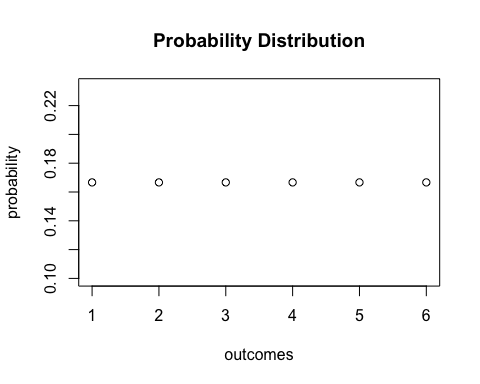
\includegraphics{URFITE_files/figure-latex/unnamed-chunk-3-1} \end{center}

For the cumulative probability distribution we need the cumulative
probabilities i.e.~we need the cumulative sums of the vector
\texttt{probability}. These sums can be computed using
\texttt{cumsum()}.

\begin{Shaded}
\begin{Highlighting}[]
\CommentTok{#generate the vector of cumulative probabilities }
\NormalTok{cum_probability <-}\StringTok{ }\KeywordTok{cumsum}\NormalTok{(probability) }

\CommentTok{# plot the probabilites }
\KeywordTok{plot}\NormalTok{(cum_probability, }
     \DataTypeTok{xlab =} \StringTok{"outcomes"}\NormalTok{, }
     \DataTypeTok{main =} \StringTok{"Cumulative Probability Distribution"}
\NormalTok{     ) }
\end{Highlighting}
\end{Shaded}

\begin{center}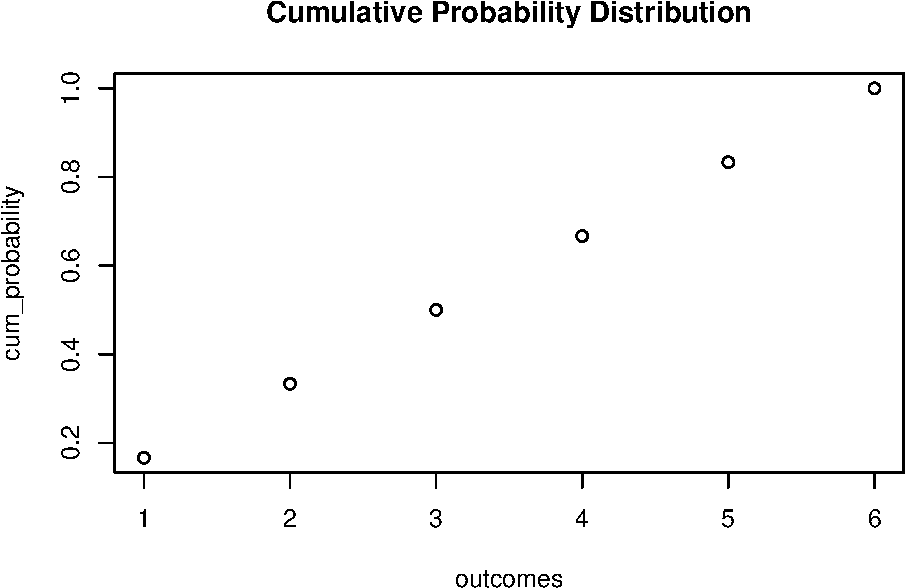
\includegraphics{URFITE_files/figure-latex/unnamed-chunk-4-1} \end{center}

\subsection*{Bernoulli Trials}\label{bernoulli-trials}
\addcontentsline{toc}{subsection}{Bernoulli Trials}

The set of elements \texttt{sample()} draws from does not have to
consist of numbers only. We might as well simulate coin tossing with
outcomes \(H\) (head) and \(T\) (tail).

\begin{Shaded}
\begin{Highlighting}[]
\KeywordTok{sample}\NormalTok{(}\KeywordTok{c}\NormalTok{(}\StringTok{"H"}\NormalTok{,}\StringTok{"T"}\NormalTok{),}\DecValTok{1}\NormalTok{) }
\end{Highlighting}
\end{Shaded}

\begin{verbatim}
## [1] "H"
\end{verbatim}

The result of a coin toss is a Bernoulli distributed random variable
i.e.~a variable with to possible distinct outcomes.

Imagine you are about to toss a coin \(10\) times in a row and wonder
how likely it is to end up with a sequence of outcomes like

\[ H \, H \, T \, T \,T \,H \,T \,T \, H \, H .\]

This is a typical example of a Bernoulli experiment as it consists of
\(n=10\) Bernoulli trials that are independent of each other and we are
interested in the likelihood of observing \(k=5\) successes \(H\) that
occur with probability \(p=0.5\) (assuming a fair coin) in each trial.

It is a well known result that the number of successes \(k\) follows a
binomial distribution

\[ k \sim B(n,p). \]

The probability of observing \(k\) successes in the experiment
\(B(n,p)\) is hence given by

\[f(k)=P(k)=\begin{pmatrix}n\\ k \end{pmatrix} \cdot p^k \cdot
q^{n-k}=\frac{n!}{k!(n-k)!} \cdot p^k \cdot q^{n-k}\]

where \(\begin{pmatrix}n\\ k \end{pmatrix}\) is a binomial coefficient.

In R, we can solve the problem stated above by means of the function
\texttt{dbinom()} which calculates the probability of the binomial
distribution for parameters \texttt{x}, \texttt{size}, and
\texttt{prob}, see \texttt{?binom}.

\begin{Shaded}
\begin{Highlighting}[]
\KeywordTok{dbinom}\NormalTok{(}\DataTypeTok{x =} \DecValTok{5}\NormalTok{,}
       \DataTypeTok{size =} \DecValTok{10}\NormalTok{,}
       \DataTypeTok{prob =} \FloatTok{0.5}
\NormalTok{       ) }
\end{Highlighting}
\end{Shaded}

\begin{verbatim}
## [1] 0.2460938
\end{verbatim}

We conclude that the probability of observing Head \(k=5\) times when
tossing the coin \(n=10\) times is about \(24.6\%\).

Now assume we are interested in \(P(4 \leq k \leq 7)\) i.e.~the
probability of observing \(4\), \(5\), \(6\) or \(7\) successes for
\(B(10,0.5)\). This is easily computed by providing a vector as the
\texttt{x} argument in our call of \texttt{dbinom()} and summing up
using \texttt{sum()}.

\begin{Shaded}
\begin{Highlighting}[]
\KeywordTok{sum}\NormalTok{(}
  \KeywordTok{dbinom}\NormalTok{(}\DataTypeTok{x =} \DecValTok{4}\OperatorTok{:}\DecValTok{7}\NormalTok{, }
         \DataTypeTok{size =} \DecValTok{10}\NormalTok{, }
         \DataTypeTok{prob =} \FloatTok{0.5}
\NormalTok{         )}
\NormalTok{  )}
\end{Highlighting}
\end{Shaded}

\begin{verbatim}
## [1] 0.7734375
\end{verbatim}

The Probability distribution of a discrete random variable is nothing
but a list of all possible outcomes that can occur and their respective
probabilities. In our coin tossing example, we face \(11\) possible
outcomes for \(k\)

\begin{Shaded}
\begin{Highlighting}[]
\CommentTok{# set up vector of possible outcomes}
\NormalTok{k <-}\StringTok{ }\DecValTok{0}\OperatorTok{:}\DecValTok{10}
\end{Highlighting}
\end{Shaded}

To visualize the probability distribution function of \(k\) we may
therefore simply call

\begin{Shaded}
\begin{Highlighting}[]
\CommentTok{# assign probabilities}
\NormalTok{probability <-}\StringTok{ }\KeywordTok{dbinom}\NormalTok{(}\DataTypeTok{x =}\NormalTok{ k,}
                      \DataTypeTok{size =} \DecValTok{10}\NormalTok{, }
                      \DataTypeTok{prob =} \FloatTok{0.5}
\NormalTok{                      )}

\CommentTok{# plot outcomes against probabilities}
\KeywordTok{plot}\NormalTok{(}\DataTypeTok{x =}\NormalTok{ k, }
     \DataTypeTok{y =}\NormalTok{ probability,}
     \DataTypeTok{main =} \StringTok{"Probability Distribution Function"}\NormalTok{) }
\end{Highlighting}
\end{Shaded}

\begin{center}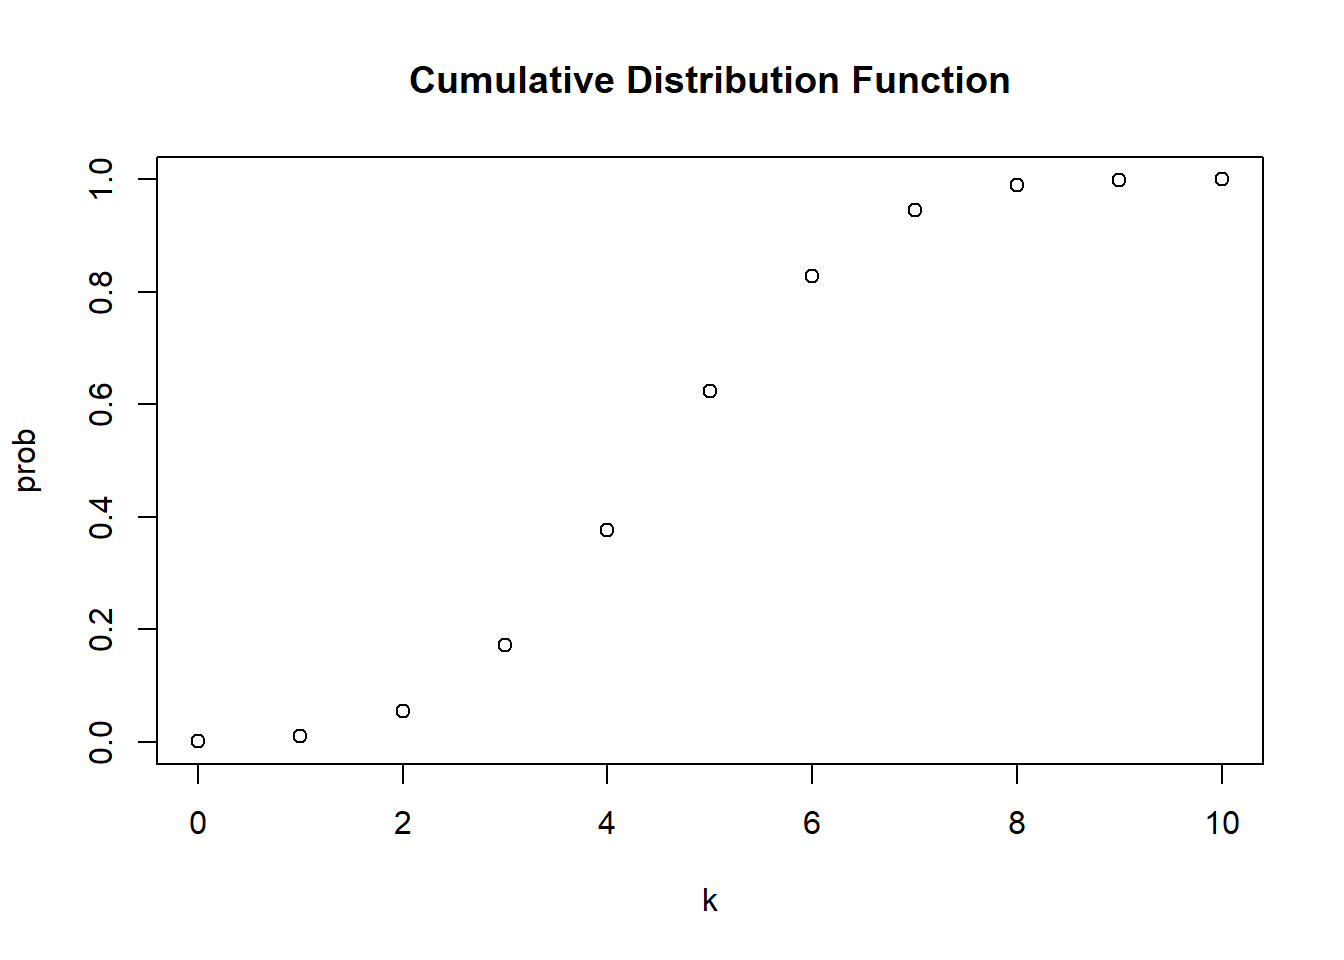
\includegraphics{URFITE_files/figure-latex/unnamed-chunk-9-1} \end{center}

In a similar fashion we may plot the cumulative distribution function of
\(k\) by executing the following code chunk:

\begin{Shaded}
\begin{Highlighting}[]
\NormalTok{prob <-}\StringTok{ }\KeywordTok{cumsum}\NormalTok{(}
              \KeywordTok{dbinom}\NormalTok{(}\DataTypeTok{x =}\DecValTok{0}\OperatorTok{:}\DecValTok{10}\NormalTok{, }
                     \DataTypeTok{size =} \DecValTok{10}\NormalTok{, }
                     \DataTypeTok{prob =} \FloatTok{0.5}
\NormalTok{                     )}
\NormalTok{              )}

\NormalTok{k <-}\StringTok{ }\DecValTok{0}\OperatorTok{:}\DecValTok{10} 
\KeywordTok{plot}\NormalTok{(}\DataTypeTok{x =}\NormalTok{ k, }
     \DataTypeTok{y =}\NormalTok{ prob,}
     \DataTypeTok{main =} \StringTok{"Cumulative Distribution Function"}\NormalTok{) }
\end{Highlighting}
\end{Shaded}

\begin{center}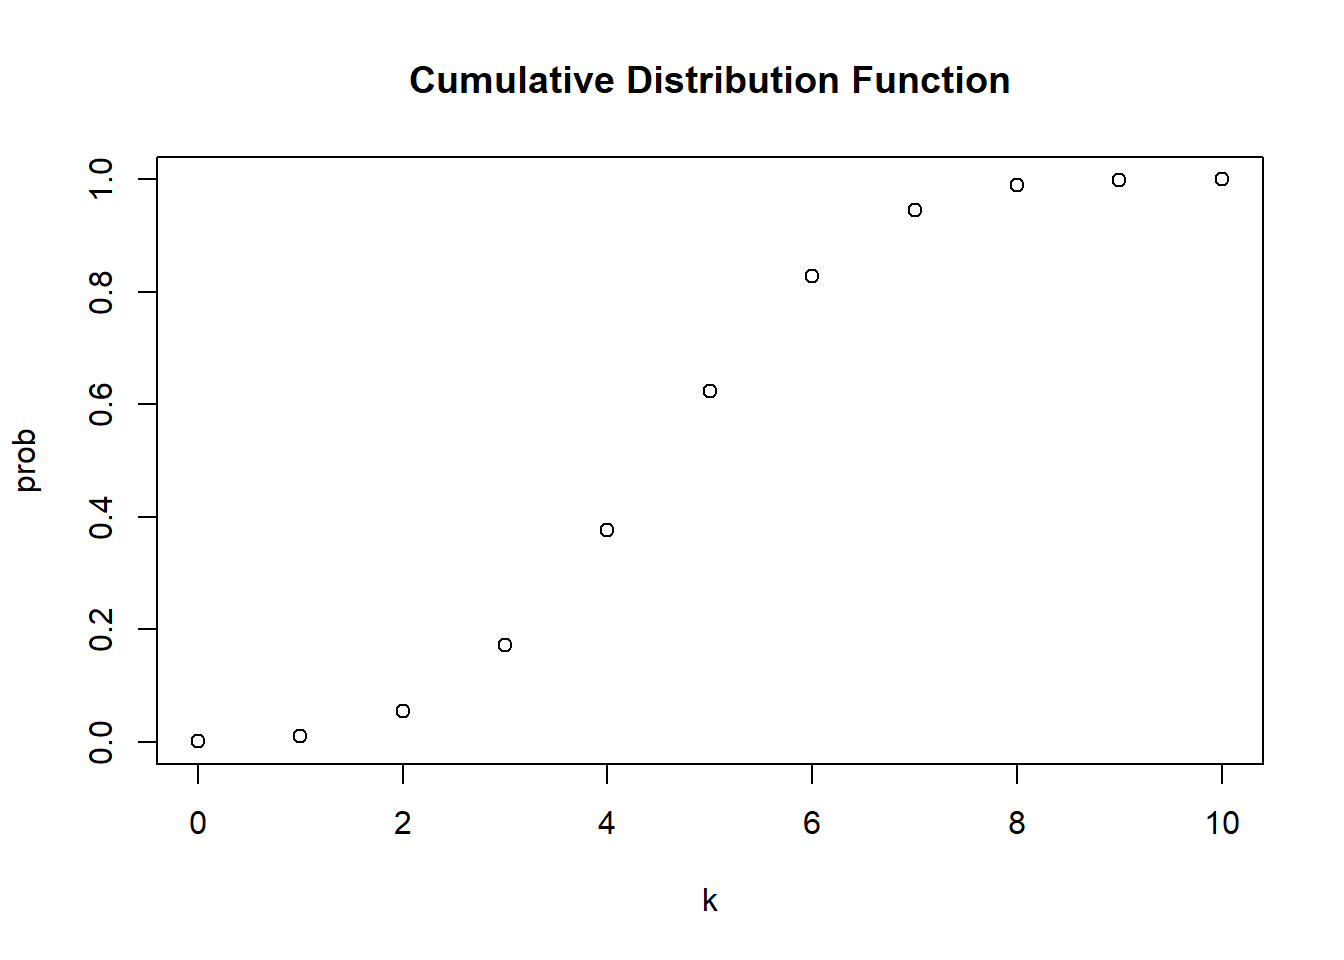
\includegraphics{URFITE_files/figure-latex/unnamed-chunk-10-1} \end{center}

\subsection*{Expected Values, Mean and
Variance}\label{expected-values-mean-and-variance}
\addcontentsline{toc}{subsection}{Expected Values, Mean and Variance}

The expected value of a random variable is the long-run average value of
the random variable over many repeated trials. For a discrete random
variable, the expected value is computed as a weighted average of its
possible outcomes whereby the weights are the related probabilities.
This is formalized in Key Concept 2.1.

Key Concept 2.1

Expected Value and the Mean

Suppose the random variable \(Y\) takes on \(k\) possible values,
\(y_1, \dots, y_k\), where \(y_1\) denotes the first value, \(y_2\)
denotes the second value, and so forth, and that the probability that
\(Y\) takes on \(y_1\) is \(p_1\), the probability that \(Y\) takes on
\(y_2\) is \(p_2\) and so forth. The expected value of \(Y\), \(E(Y)\)
is defined as

\[ E(Y) = y_1 p_1 + y_2 p_2 + \cdots + y_k p_k = \sum_{i=1}^k y_i p_i \]

where the notation \(\sum_{i=1}^k y_i p_i\) means ``the sum of \(y_i\)
\(p_i\) for \(i\) running from \(1\) to \(k\)''. The expected value of
\(Y\) is also called the mean of \(Y\) or the expectation of \(Y\) and
is denoted by \(\mu_y\).

In the dice example, the random variable, \(D\) say, takes on \(6\)
possible values \(d_1 = 1, d_2 = 2, \dots, d_6 = 6\). Assuming a fair
dice, each of the \(6\) outcomes occurs with a probability of \(1/6\).
It is therefore easy to calculate the exact value of \(E(D)\) by hand:

\[ E(D) = 1/6 \sum_{i=1}^6 d_i = 3.5 \]

Here, this is simply the average of the natural numbers from \(1\) to
\(6\) since all wights \(p_i\) are \(1/6\). Convince Yourself that this
can be easily calculated using the function \texttt{mean()} which
computes the arithmetic mean of a numeric vector.

\begin{Shaded}
\begin{Highlighting}[]
\KeywordTok{mean}\NormalTok{(}\DecValTok{1}\OperatorTok{:}\DecValTok{6}\NormalTok{)}
\end{Highlighting}
\end{Shaded}

\begin{verbatim}
## [1] 3.5
\end{verbatim}

An example of sampling with replacement is rolling a dice three times in
a row.

\begin{Shaded}
\begin{Highlighting}[]
\CommentTok{# set random seed for reproducibility}
\KeywordTok{set.seed}\NormalTok{(}\DecValTok{1}\NormalTok{)}

\CommentTok{# rolling a dice three times in a row}
\KeywordTok{sample}\NormalTok{(}\DecValTok{1}\OperatorTok{:}\DecValTok{6}\NormalTok{, }\DecValTok{3}\NormalTok{, }\DataTypeTok{replace =}\NormalTok{ T)}
\end{Highlighting}
\end{Shaded}

\begin{verbatim}
## [1] 2 3 4
\end{verbatim}

Of course we could also consider a much bigger number of trials,
\(10000\) say. Doing so, it would be pointless to simply print the
results to the console: by default R displays up to \(1000\) entries of
large vectors and omitts the remainder (give it a go). Eyeballing the
numbers does not reveal too much. Instead let us calculate the sample
average of the outcomes using \texttt{mean()} and see if the result
comes close to the expected value \(E(D)=3.5\).

\begin{Shaded}
\begin{Highlighting}[]
\CommentTok{# set random seed for reproducibility}
\KeywordTok{set.seed}\NormalTok{(}\DecValTok{1}\NormalTok{)}

\CommentTok{# compute the sample mean of 10000 die rolls}
\KeywordTok{mean}\NormalTok{(}
    \KeywordTok{sample}\NormalTok{(}\DecValTok{1}\OperatorTok{:}\DecValTok{6}\NormalTok{, }
           \DecValTok{10000}\NormalTok{, }
           \DataTypeTok{replace =}\NormalTok{ T}
\NormalTok{           )}
\NormalTok{    )}
\end{Highlighting}
\end{Shaded}

\begin{verbatim}
## [1] 3.5039
\end{verbatim}

We find the sample mean to be fairly close to the expected value. (ref
to WLLN)

Other frequently encountered measures are the variance and the standard
deviation. Both are measures of the \emph{dispersion} of a random
variable.

Key Concept 2.2

Variance and Standard Deviation

The Variance of the discrete \emph{random variable} \(Y\), denoted
\(\sigma^2_Y\), is
\[ \sigma^2_Y = \text{Var}(Y) = E\left[(Y-\mu_y)^2\right] = \sum_{i=1}^k (y_i - \mu_y)^2 p_i \]
The standard deviation of \(Y\) is \(\sigma_Y\), the square root of the
variance. The units of the standard deviation are the same as the units
of \(Y\).

The variance as defined in Key Concept 2.2 \emph{is not} implemented as
a function in R. Instead we have the function \texttt{var()} which
computes the \emph{sample variance}

\[ s^2_Y = \frac{1}{n-1} \sum_{i=1}^n (y_i - \overline{y})^2. \]

Remember that \(s^2_Y\) is different from the so called \emph{population
variance} of \(Y\),

\[ \text{Var}(Y) = \frac{1}{N} \sum_{i=1}^N (y_i - \mu_Y)^2, \]

since it measures how the data is dispersed around the sample average
\(\overline{y}\) instead of the population mean \(\mu_Y\). This becomes
clear when we look at our dice rolling example. For \(D\) we have

\[ \text{Var}(D) = 1/6 \sum_{i=1}^6 (d_i - 3.5)^2 = 2.92  \] which is
obviously different from the result of \(s^2\) as computed by
\texttt{var()}.

\begin{Shaded}
\begin{Highlighting}[]
\KeywordTok{var}\NormalTok{(}\DecValTok{1}\OperatorTok{:}\DecValTok{6}\NormalTok{)}
\end{Highlighting}
\end{Shaded}

\begin{verbatim}
## [1] 3.5
\end{verbatim}

\section{Probability Distributions of Continuous Random
Variables}\label{probability-distributions-of-continuous-random-variables}

Since a continuous random variable takes on a continuum of possible
values, we cannot use the concept of a probability distribution as used
for discrete random variables. Instead, the probability distribution of
a continuous random variable is summarized by its \emph{probability
density function} (PDF).

The cumulative probability distribution function (CDF) for a continuous
random variable is defined just as in the discrete case. Hence, the
cumulative probability distribution of a continuous random variables
states the probability that the random variable is less than or equal to
a particular value.

For completeness, we present revisions of Key Concepts 2.1 and 2.2 for
the continuous case.

Key Concept 2.3

Probabilities, Expected Value and Variance of a Continuous Random
Variable

Let \(f_Y(y)\) denote the probability density function of \(Y\). Because
probabilities cannot be negative, we have \(f_Y\geq 0\) for all \(y\).
The Probability that \(Y\) falls between \(a\) and \(b\), \(a < b\) is
\[ P(a \leq Y \leq b) = \int_a^b f_Y(y) \mathrm{d}y. \] We further have
that \(P(-\infty \leq Y \leq \infty) = 1\) and therefore
\(\int_{-\infty}^{\infty} f_Y(y) \mathrm{d}y = 1\).

As for the discrete case, the expected value of \(Y\) is the probability
weighted average of its values. Due to continuity, we use intergrals
instead of sums.

The expected value of \(Y\) is

\[ E(Y) =  \mu_Y = \int y f_Y(y) \mathrm{d}y. \]

The variance is the expected value of \((Y - \mu_Y)^2\). We thus have

\[ \text{Var}(Y) =  \sigma_Y^2 = \int (y - \mu_Y)^2 f_Y(y) \mathrm{d}y. \]

Let us discuss an example:

Consider the continuous random variable \(X\) with propability density
function

\[ f_X(x) = \frac{3}{x^4}, x>1. \]

\begin{itemize}
\tightlist
\item
  We can show analytically that the integral of \(f_X(x)\) over the real
  line equals \(1\).
\end{itemize}

\begin{align}
 \int f_X(x) \mathrm{d}x =&  \int_{1}^{\infty} \frac{3}{x^4} \mathrm{d}x \\
  =& \lim_{t \rightarrow \infty} \int_{1}^{t} \frac{3}{x^4} \mathrm{d}x \\
  =& \lim_{t \rightarrow \infty}  -x^{-3} \rvert_{x=1}^t \\
  =& -\left(\lim_{t \rightarrow \infty}\frac{1}{t^3} - 1\right) \\
  =& 1
\end{align}

\begin{itemize}
\tightlist
\item
  The expectation of \(X\) can be computed as follows:
\end{itemize}

\begin{align}
 E(X) = \int x \cdot f_X(x) \mathrm{d}x =&  \int_{1}^{\infty} x \cdot \frac{3}{x^4} \mathrm{d}x \\
  =& - \frac{3}{2} x^{-2} \rvert_{x=1}^{\infty} \\
  =& -\frac{3}{2} \left( \lim_{t \rightarrow \infty} \frac{1}{t^2} - 1 \right) \\
  =& \frac{3}{2}
\end{align}

\begin{itemize}
\tightlist
\item
  Note that the variance of \(X\) can be expressed as
  \(\text{Var}(X) = E(X^2) - E(X)^2\). Since \(E(X)\) has been computed
  in the previous step, we seek \(E(X^2)\):
\end{itemize}

\begin{align}
 E(X^2)= \int x^2 \cdot f_X(x) \mathrm{d}x =&  \int_{1}^{\infty} x^2 \cdot \frac{3}{x^4} \mathrm{d}x \\
  =& -3 x^{-1} \rvert_{x=1}^{\infty} \\
  =& -3 \left( \lim_{t \rightarrow \infty} \frac{1}{t} - 1 \right) \\
  =& 3
\end{align}

So we have shown that the area under the curve equals one, that the
expectation is \(E(X)=\frac{3}{2} \ \) and we found the variance to be
\(\text{Var}(X) = \frac{3}{4}\). However, this was quite tedious and, as
we shall see soon, an analytic approach is not applicable for some
probability density functions e.g.~if integrals have no closed form
solutions.

Luckily, R enables us to find the results derived above in an instant.
The tool we use for this is the function \texttt{integrate()}. First, we
have to define the functions we want to calculate integrals for as R
functions, i.e.~the PDF \(f_X(x)\) as well as the expressions
\(x\cdot f_X(x)\) and \(x^2\cdot f_X(x)\).

\begin{Shaded}
\begin{Highlighting}[]
\CommentTok{# define functions}
\NormalTok{f <-}\StringTok{ }\ControlFlowTok{function}\NormalTok{(x) }\DecValTok{3}\OperatorTok{/}\NormalTok{x}\OperatorTok{^}\DecValTok{4}
\NormalTok{g <-}\StringTok{ }\ControlFlowTok{function}\NormalTok{(x) x}\OperatorTok{*}\KeywordTok{f}\NormalTok{(x)}
\NormalTok{h <-}\StringTok{ }\ControlFlowTok{function}\NormalTok{(x) x}\OperatorTok{^}\DecValTok{2}\OperatorTok{*}\KeywordTok{f}\NormalTok{(x)}
\end{Highlighting}
\end{Shaded}

Next, we use \texttt{integrate()} and set lower and upper limits of
integration to \(1\) and \(\infty\) using arguments \texttt{lower} and
\texttt{upper}. By default, \texttt{integrate()} prints the result along
with an estimate of the calculation error to the console. However, the
outcome is not a numeric value one can do further calculation with
readily. In order to get only a numeric value of the integral, we need
to use the \texttt{\$} operator in conjunction with \texttt{value}.

\begin{Shaded}
\begin{Highlighting}[]
\CommentTok{# calculate area under curve}
\NormalTok{AUC <-}\StringTok{ }\KeywordTok{integrate}\NormalTok{(f, }
                 \DataTypeTok{lower =} \DecValTok{1}\NormalTok{, }
                 \DataTypeTok{upper =} \OtherTok{Inf}
\NormalTok{                 )}
\NormalTok{AUC }
\end{Highlighting}
\end{Shaded}

\begin{verbatim}
## 1 with absolute error < 1.1e-14
\end{verbatim}

\begin{Shaded}
\begin{Highlighting}[]
\CommentTok{# calculate E(X)}
\NormalTok{EX <-}\StringTok{ }\KeywordTok{integrate}\NormalTok{(g,}
                \DataTypeTok{lower =} \DecValTok{1}\NormalTok{,}
                \DataTypeTok{upper =} \OtherTok{Inf}\NormalTok{)}
\NormalTok{EX}
\end{Highlighting}
\end{Shaded}

\begin{verbatim}
## 1.5 with absolute error < 1.7e-14
\end{verbatim}

\begin{Shaded}
\begin{Highlighting}[]
\CommentTok{# calculate Var(X)}
\NormalTok{VarX <-}\StringTok{ }\KeywordTok{integrate}\NormalTok{(h,}
                  \DataTypeTok{lower =} \DecValTok{1}\NormalTok{,}
                  \DataTypeTok{upper =} \OtherTok{Inf}
\NormalTok{                  )}\OperatorTok{$}\NormalTok{value }\OperatorTok{-}\StringTok{ }\NormalTok{EX}\OperatorTok{$}\NormalTok{value}\OperatorTok{^}\DecValTok{2} 
\NormalTok{VarX}
\end{Highlighting}
\end{Shaded}

\begin{verbatim}
## [1] 0.75
\end{verbatim}

Although there is a wide variety of distributions, the ones most often
encountered in econometrics are the normal, chi-squared, Student \(t\)
and \(F\) distributions. Therefore we will discuss some core R functions
that allow to do calculations involving densities, probabilities and
quantiles of these distributions.

Every probability distribution that R handles has four basic functions
whose names consist of a prefix followed by a root name. As an example,
take the normal distribution. The root name of all four functions
associated with the normal distribution is norm. The four prefixes are

\begin{itemize}
\tightlist
\item
  d for ``density'' - probability function / probability density
  function
\item
  p for ``probability'' - cumulative distribution function
\item
  q for ``quantile'' - quantile function (inverse cumulative
  distribution function)
\item
  r for ``random'' - random number generator
\end{itemize}

Thus, for the normal distribution we have the R functions
\texttt{dnorm()}, \texttt{pnorm()}, \texttt{qnorm()} and
\texttt{rnorm()}.

\subsection*{The Normal Distribution}\label{the-normal-distribution}
\addcontentsline{toc}{subsection}{The Normal Distribution}

The probably most important probability distribution considered here is
the normal distribution. This is not least due to the special role of
the standard normal distribution and the Central Limit Theorem which is
treated shortly during the course of this section. Distributions of the
normal family have a familiar symmetric, bell-shaped probability
density. A normal distribution is characterized by its mean \(\mu\) and
its standard deviation \(\sigma\) what is concisely expressed by
\(N(\mu,\sigma^2)\). The normal distribution has the PDF

\[ f(x) = \frac{1}{\sqrt{2 \pi} \sigma} e^{-(x - μ)^2/(2 σ^2)}. \]

For the standard normal distribution we have \(\mu=0\) and \(\sigma=1\).
Standard normal variates are often denoted \(Z\). Usually, the standard
normal PDF is denoted by \(\phi\) and the standard normal CDF is denoted
by \(\Phi\). Hence,

\[ \phi(c) = \Phi'(c) \ \ , \ \ \Phi(c) = P(Z \leq c) \ \ , \ \ Z \sim N(0,1).
\] In R, we can conveniently obtain density values of normal
distributions using the function \texttt{dnorm()}. Let us draw a plot of
the standard normal density function using \texttt{curve()} and
\texttt{dnorm()}.

\begin{Shaded}
\begin{Highlighting}[]
\CommentTok{# draw a plot of the N(0,1) pdf}
\KeywordTok{curve}\NormalTok{(}\KeywordTok{dnorm}\NormalTok{(x),}
      \DataTypeTok{xlim=}\KeywordTok{c}\NormalTok{(}\OperatorTok{-}\FloatTok{3.5}\NormalTok{, }\FloatTok{3.5}\NormalTok{),}
      \DataTypeTok{ylab =} \StringTok{"Density"}\NormalTok{, }
      \DataTypeTok{main =} \StringTok{"Standard Normal Density Function"}
\NormalTok{      ) }
\end{Highlighting}
\end{Shaded}

\begin{center}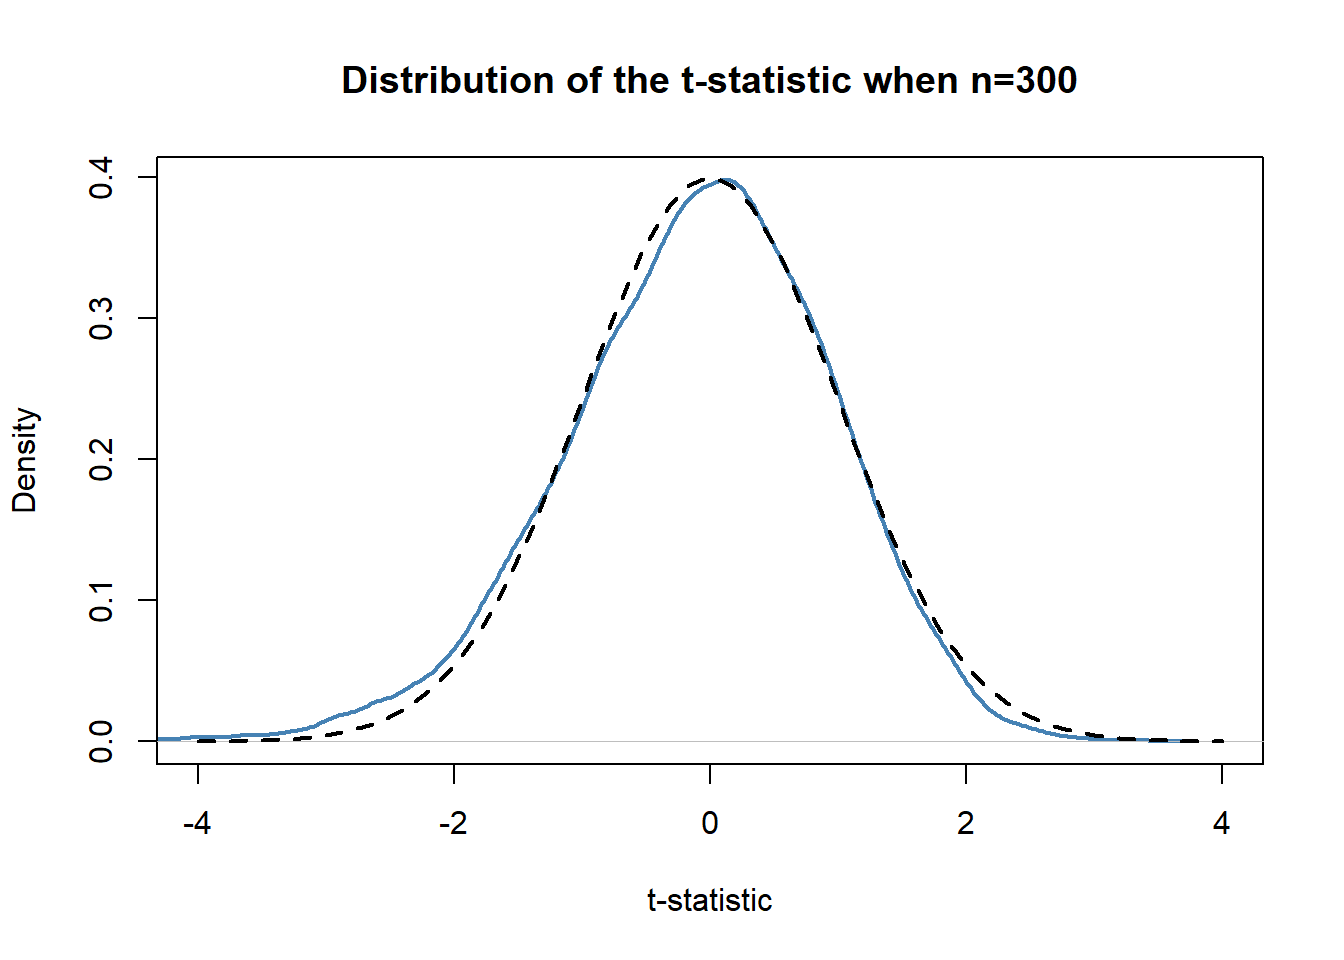
\includegraphics{URFITE_files/figure-latex/unnamed-chunk-17-1} \end{center}

We can obtain the density at different positions by passing a vector of
quantiles to \texttt{dnorm()}.

\begin{Shaded}
\begin{Highlighting}[]
\CommentTok{# compute denstiy at x=-1.96, x=0 and x=1.96}
\KeywordTok{dnorm}\NormalTok{(}\DataTypeTok{x =} \KeywordTok{c}\NormalTok{(}\OperatorTok{-}\FloatTok{1.96}\NormalTok{, }\DecValTok{0}\NormalTok{, }\FloatTok{1.96}\NormalTok{))}
\end{Highlighting}
\end{Shaded}

\begin{verbatim}
## [1] 0.05844094 0.39894228 0.05844094
\end{verbatim}

Similary as for the PDF, we can plot the standard normal CDF using
\texttt{curve()} and \texttt{pnorm()}.

\begin{Shaded}
\begin{Highlighting}[]
\CommentTok{# plot the standard normal CDF}
\KeywordTok{curve}\NormalTok{(}\KeywordTok{pnorm}\NormalTok{(x), }
      \DataTypeTok{xlim=}\KeywordTok{c}\NormalTok{(}\OperatorTok{-}\FloatTok{3.5}\NormalTok{, }\FloatTok{3.5}\NormalTok{), }
      \DataTypeTok{ylab =} \StringTok{"Density"}\NormalTok{, }
      \DataTypeTok{main =} \StringTok{"Standard Normal Cumulative Distribution Function"}
\NormalTok{      )}
\end{Highlighting}
\end{Shaded}

\begin{center}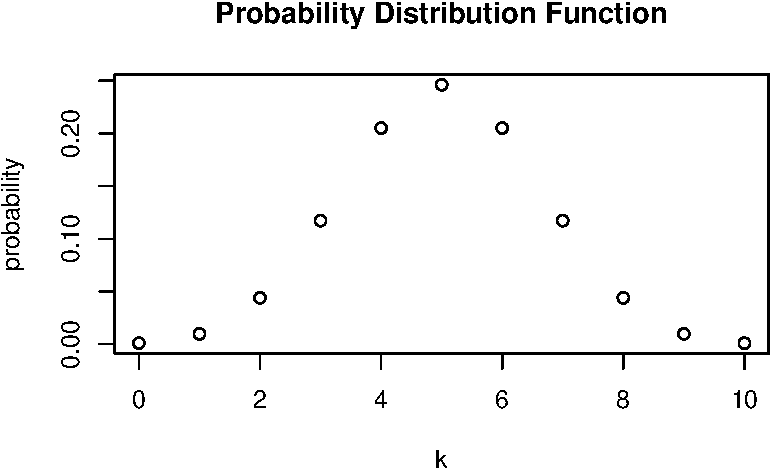
\includegraphics{URFITE_files/figure-latex/unnamed-chunk-19-1} \end{center}

We can also use R to calculate the probability of events associated with
a standard normal random variate.

Let us say we are interested in \(P(Z \leq 1.337)\). For some general
continuous random variable \(Z\) on \([-\infty,\infty]\) with density
function \(g(x)\) we would have to determine \(G(x)\), the
antiderivative of \(g(x)\) since

\[ P(Z \leq 1,337 ) = G(1,337) = \int_{-\infty}^{1,337} g(x) \mathrm{d}x.  \]

However, if \(Z \sim N(0,1)\), we have \(g(x)=\phi(x)\) so there is no
analytic solution to the integral above and it is cumbersome to come up
with an approximation. However, we may circumvent this using R in
different ways. The first approach makes use of the function
\texttt{integrate()} which allows to solve one-dimensional integration
problems using a numerical method. For this, we first define the
function we want to compute the integral of as a R function \texttt{f}.
In our example, \texttt{f} needs to be the standard normal density
function and hence takes a single argument \texttt{x}. Following the
definition of \(\phi(x)\) we define \texttt{f} as

\begin{Shaded}
\begin{Highlighting}[]
\CommentTok{# define the standard normal PDF as a R function}
\NormalTok{f <-}\StringTok{ }\ControlFlowTok{function}\NormalTok{(x) \{}
  \DecValTok{1}\OperatorTok{/}\NormalTok{(}\KeywordTok{sqrt}\NormalTok{(}\DecValTok{2} \OperatorTok{*}\StringTok{ }\NormalTok{pi)) }\OperatorTok{*}\StringTok{ }\KeywordTok{exp}\NormalTok{(}\OperatorTok{-}\FloatTok{0.5} \OperatorTok{*}\StringTok{ }\NormalTok{x}\OperatorTok{^}\DecValTok{2}\NormalTok{)}
\NormalTok{\}}
\end{Highlighting}
\end{Shaded}

Let us check if this function enables us to compute standard normal
density values by passing it a vector of quantiles.

\begin{Shaded}
\begin{Highlighting}[]
\CommentTok{# define vector of quantiles}
\NormalTok{quants <-}\StringTok{ }\KeywordTok{c}\NormalTok{(}\OperatorTok{-}\FloatTok{1.96}\NormalTok{,}\DecValTok{0}\NormalTok{,}\FloatTok{1.96}\NormalTok{)}

\CommentTok{# compute density values}
\KeywordTok{f}\NormalTok{(quants)}
\end{Highlighting}
\end{Shaded}

\begin{verbatim}
## [1] 0.05844094 0.39894228 0.05844094
\end{verbatim}

\begin{Shaded}
\begin{Highlighting}[]
\CommentTok{# compare to results produced by dnorm()}
\KeywordTok{f}\NormalTok{(quants) }\OperatorTok{==}\StringTok{ }\KeywordTok{dnorm}\NormalTok{(quants)}
\end{Highlighting}
\end{Shaded}

\begin{verbatim}
## [1] TRUE TRUE TRUE
\end{verbatim}

Notice that the results produces by \texttt{f()} are indeed equivalent
to those given by \texttt{dnorm()}.

Next, we call \texttt{integrate()} on \texttt{f()} and further specify
the arguments \texttt{lower} and \texttt{upper}, the lower and upper
limits of integration.

\begin{Shaded}
\begin{Highlighting}[]
\CommentTok{# integrate f()}
\KeywordTok{integrate}\NormalTok{(f, }
          \DataTypeTok{lower =} \OperatorTok{-}\OtherTok{Inf}\NormalTok{, }
          \DataTypeTok{upper =} \FloatTok{1.337}
\NormalTok{          )}
\end{Highlighting}
\end{Shaded}

\begin{verbatim}
## 0.9093887 with absolute error < 1.7e-07
\end{verbatim}

We find that the probability of observing \(Z \leq 1,337\) is about
\(0.9094\%\).

A second and much more convenient way is to use the function
\texttt{pnorm()} which also allows calculus involving the standard
normal cumulative distribution function.

\begin{Shaded}
\begin{Highlighting}[]
\CommentTok{# compute a probability using pnorm()}
\KeywordTok{pnorm}\NormalTok{(}\FloatTok{1.337}\NormalTok{)}
\end{Highlighting}
\end{Shaded}

\begin{verbatim}
## [1] 0.9093887
\end{verbatim}

The result matches the outcome of the approach using
\texttt{ìntegrate()}.

Let us discuss some further examples:

A commonly known result is that \(95\%\) probability mass of a standard
normal lies in the intervall \([-1.96, 1.96]\), that is in a distance of
about \(2\) standard deviations to the mean. We can easily confirm this
by calculating

\[ P(-1.96 \leq Z \leq 1.96) = 1-2\times P(Z \leq -1.96) \] due to
symmetry of the standard normal PDF. Thanks to R, we can abondon the
table of the standard normal CDF again and instead solve this by means
of the function \texttt{pnorm()}.

\begin{Shaded}
\begin{Highlighting}[]
\CommentTok{# compute the probability}
\DecValTok{1} \OperatorTok{-}\StringTok{ }\DecValTok{2} \OperatorTok{*}\StringTok{ }\NormalTok{(}\KeywordTok{pnorm}\NormalTok{(}\OperatorTok{-}\FloatTok{1.96}\NormalTok{)) }
\end{Highlighting}
\end{Shaded}

\begin{verbatim}
## [1] 0.9500042
\end{verbatim}

Now consider a random variable \(Y\) with \(Y \sim N(5,25)\). As You
should already know from Your statistics courses it is not possible to
make any statement of probability without prior standardizing as shown
in Key Concept 2.4.

Key Concept 2.4

Computing Probabilities Involving Normal Random Variables

Suppose \(Y\) is normally distributed with mean \(\mu\) and variance
\(\sigma^2\): \[Y
\sim N(\mu, \sigma^2)\] Then \(Y\) is standardized by substracting its
mean and dividing by its standard deviation:
\[ Z = \frac{Y -\mu}{\sigma} \] Let \(c_1\) and \(c_2\) denote two
numbers whereby \(c_1 < c_2\) and further \(d_1 = (c_1 - \mu) / \sigma\)
and \(d_2 = (c_2 - \mu)/\sigma\). Then

\begin{align} 
P(Y \leq c_2) =& \, P(Z \leq d_2) = \Phi(d_2) \\ 
P(Y \geq c_1) =& \, P(Z \geq d_1) = 1 - \Phi(d_1) \\ 
P(c_1 \leq Y \leq c_2) =& \, P(d_1 \leq Z \leq d_2) = \Phi(d_2) - \Phi(d_1) 
\end{align}

R functions that handle the normal distribution can perform this
standardization. If we are interested in \(P(3 \leq Y \leq 4)\) we can
use \texttt{pnorm()} and adjust for a mean and/or a standard deviation
that deviate from \(\mu=0\) and \(\sigma = 1\) by specifying the
arguments \texttt{mean} and \texttt{sd} accordingly. \textbf{Attention}:
\texttt{pnorm()} requires the argument \texttt{sd} which is the standard
deviation, not the variance!

\begin{Shaded}
\begin{Highlighting}[]
\KeywordTok{pnorm}\NormalTok{(}\DecValTok{4}\NormalTok{, }\DataTypeTok{mean =} \DecValTok{5}\NormalTok{, }\DataTypeTok{sd =} \DecValTok{5}\NormalTok{) }\OperatorTok{-}\StringTok{ }\KeywordTok{pnorm}\NormalTok{(}\DecValTok{3}\NormalTok{, }\DataTypeTok{mean =} \DecValTok{5}\NormalTok{, }\DataTypeTok{sd =} \DecValTok{5}\NormalTok{) }
\end{Highlighting}
\end{Shaded}

\begin{verbatim}
## [1] 0.07616203
\end{verbatim}

An extension of the normal distribution in a univariate setting is the
multivariate normal distribution. The PDF of two random normal variables
\(X\) and \(Y\) is given by

\begin{align}
g_{X,Y}(x,y) =& \, \frac{1}{2\pi\sigma_X\sigma_Y\sqrt{1-\rho_{XY}^2}} \\ 
\cdot & \, \exp \left\{ \frac{1}{-2(1-\rho_{XY}^2)} \left[ \left( \frac{x-\mu_x}{\sigma_x} \right)^2 - 2\rho_{XY}\left( \frac{x-\mu_X}{\sigma_X} \right)\left( \frac{y-\mu_Y}{\sigma_Y} \right) + \left( \frac{y-\mu_Y}{\sigma_Y} \right)^2 \right]  \right\}. \label{eq:bivnorm}
\end{align}

Equation \eqref{eq:bivnorm} contains the bivariate normal PDF. Admittedly,
it is hard to gain insights from this complicated expression. Instead,
let us consider the special case where \(X\) and \(Y\) are uncorrelated
standard normal random variables with density functions \(f_X(x)\) and
\(f_Y(y)\) and we assume that they have a joint normal distribution. We
then have the parameters \(\sigma_X = \sigma_Y = 1\), \(\mu_X=\mu_Y=0\)
(due to marginal standard normality) and \(\rho_{XY}=0\) (due to
uncorrelatedness). The joint probability density function of \(X\) and
\(Y\) then becomes

\[ g_{X,Y}(x,y) = f_X(x) f_Y(y) = \frac{1}{2\pi} \cdot \exp \left\{ -\frac{1}{2} \left[x^2 + y^2 \right]  \right\}, \tag{2.2}  \]

the PDF of the bivariate standard normal distribution. The next plot
provides an interactive three dimensional plot of (2.2). By moving the
mouse curser over the plot You can see that the density is rotationally
invariant.

\subsection*{The Chi-Squared
Distribution}\label{the-chi-squared-distribution}
\addcontentsline{toc}{subsection}{The Chi-Squared Distribution}

Another distribution relevant in econometric day-to-day work is the
chi-squared distribution. It is often needed when testing special types
of hypotheses frequently ecountered when dealing with regression models.

The sum of \(M\) squared independent standard normal distributed random
variables follows a chi-squared distribution with \(M\) degrees of
freedom.

\[ Z_1^2 + \dots + Z_M^2 = \sum_{m=1}^M Z_m^2 \sim \chi^2_M \ \ \text{with} \ \ Z_m \overset{i.i.d.}{\sim} N(0,1) \label{eq:chisq}\]

A \(\chi^2\) distributed random variable with \(M\) degrees of freedom
has expectation \(M\), mode at \(M-2\) for \(n \geq 2\) and variance
\(2 \cdot M\).

For example, if we have

\[ Z_1,Z_2,Z_3 \overset{i.i.d.}{\sim} N(0,1) \]

it holds that

\[ Z_1^2+Z_2^2+Z_3^3 \sim \chi^2_3. \tag{2.3} \] By means of the code
below, we can display the PDF and the CDF of a \(\chi^2_3\) random
variable in a single plot. This is achieved by setting the argument
\texttt{add\ =\ TRUE} in the second call of \texttt{curve()}. Further we
adjust limits of both axes using \texttt{xlim} and \texttt{ylim} and
choose different colors to make both functions better distinguishable.
The plot is completed by adding a legend with help of the function
\texttt{legend()}.

\begin{Shaded}
\begin{Highlighting}[]
\CommentTok{# plot the PDF}
\KeywordTok{curve}\NormalTok{(}\KeywordTok{dchisq}\NormalTok{(x, }\DataTypeTok{df=}\DecValTok{3}\NormalTok{), }
      \DataTypeTok{xlim=}\KeywordTok{c}\NormalTok{(}\DecValTok{0}\NormalTok{,}\DecValTok{10}\NormalTok{), }
      \DataTypeTok{ylim =} \KeywordTok{c}\NormalTok{(}\DecValTok{0}\NormalTok{,}\DecValTok{1}\NormalTok{), }
      \DataTypeTok{col=}\StringTok{"blue"}\NormalTok{, }
      \DataTypeTok{main=}\StringTok{"p.d.f. and c.d.f of Chi-Squared Distribution, m = 3"}
\NormalTok{      )}

\CommentTok{# add the CDF to the plot}
\KeywordTok{curve}\NormalTok{(}\KeywordTok{pchisq}\NormalTok{(x, }\DataTypeTok{df=}\DecValTok{3}\NormalTok{), }
      \DataTypeTok{xlim=}\KeywordTok{c}\NormalTok{(}\DecValTok{0}\NormalTok{,}\DecValTok{10}\NormalTok{), }
      \DataTypeTok{add =} \OtherTok{TRUE}\NormalTok{, }
      \DataTypeTok{col=}\StringTok{"red"}
\NormalTok{      )}

\CommentTok{# add a legend to the plot}
\KeywordTok{legend}\NormalTok{(}\StringTok{"topleft"}\NormalTok{, }
       \KeywordTok{c}\NormalTok{(}\StringTok{"PDF"}\NormalTok{,}\StringTok{"CDF"}\NormalTok{), }
       \DataTypeTok{col =} \KeywordTok{c}\NormalTok{(}\StringTok{"blue"}\NormalTok{,}\StringTok{"red"}\NormalTok{), }
       \DataTypeTok{lty =} \KeywordTok{c}\NormalTok{(}\DecValTok{1}\NormalTok{,}\DecValTok{1}\NormalTok{)}
\NormalTok{       )}
\end{Highlighting}
\end{Shaded}

\begin{center}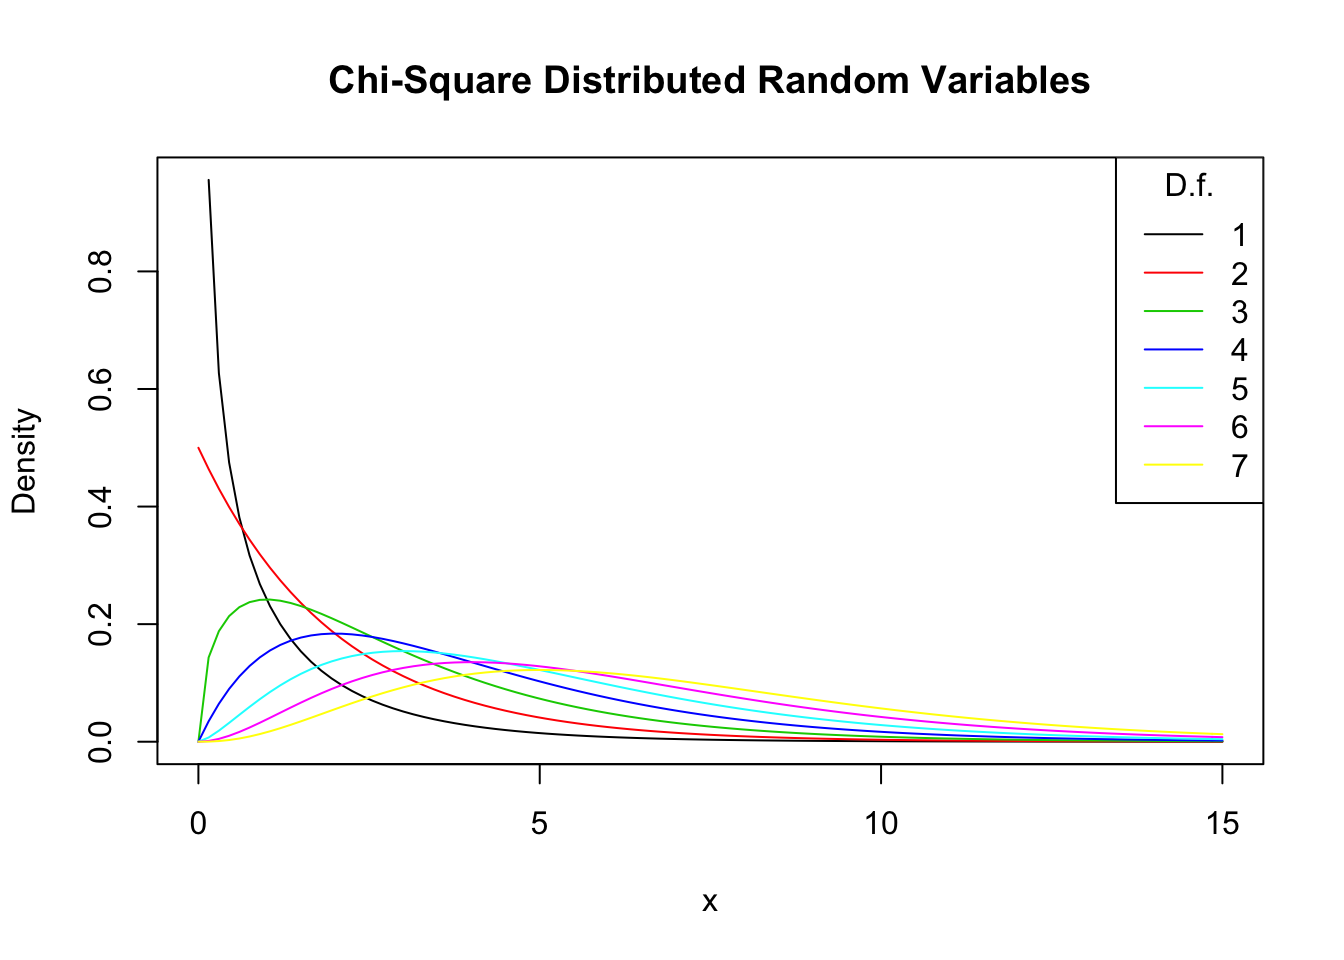
\includegraphics{URFITE_files/figure-latex/unnamed-chunk-27-1} \end{center}

Notice that, since the outcomes of a \(\chi^2_M\) distributed random
variable are always positive, the domain of the related PDF and CDF is
\(\mathbb{R}_{\geq0}\).

As expectation and variance depend (solely) on the degrees of freedom,
the distribution's shape changes drastically if we vary the number of
squared standard normals that are summed up. This relation is often
depicted by overlaying densities for different \(M\), see e.g.~the
Wikipedia Article.

Of course, one can easily reproduce such a plot using R. Again we start
by plotting the density of the \(\chi_1^2\) distribution on the
intervall \([0,15]\) with \texttt{curve()}. In the next step, we loop
over degrees of freedom \(m=2,...,7\) and add a density curve for each
\(m\) to the plot. We also adjust the line color for each iteration of
the loop by setting \texttt{col\ =\ m}. At last, we add a legend that
displays degrees of freedom and the associated colors.

\begin{Shaded}
\begin{Highlighting}[]
\CommentTok{# plot the density for m=1}
\KeywordTok{curve}\NormalTok{(}\KeywordTok{dchisq}\NormalTok{(x, }\DataTypeTok{df=}\DecValTok{1}\NormalTok{), }
      \DataTypeTok{xlim=}\KeywordTok{c}\NormalTok{(}\DecValTok{0}\NormalTok{,}\DecValTok{15}\NormalTok{), }
      \DataTypeTok{xlab =} \StringTok{"x"}\NormalTok{, }
      \DataTypeTok{ylab =} \StringTok{"Density"}\NormalTok{, }
      \DataTypeTok{main=}\StringTok{"Chi-Square Distributed Random Variables"}
\NormalTok{      )}

\CommentTok{# add densities for m=2,...,7 to the plot using a for loop }
\ControlFlowTok{for}\NormalTok{ (m }\ControlFlowTok{in} \DecValTok{2}\OperatorTok{:}\DecValTok{7}\NormalTok{) \{}
  \KeywordTok{curve}\NormalTok{(}\KeywordTok{dchisq}\NormalTok{(x, }\DataTypeTok{df =}\NormalTok{ m),}
        \DataTypeTok{xlim =} \KeywordTok{c}\NormalTok{(}\DecValTok{0}\NormalTok{,}\DecValTok{15}\NormalTok{), }
        \DataTypeTok{add =}\NormalTok{ T, }
        \DataTypeTok{col =}\NormalTok{ m}
\NormalTok{        )}
\NormalTok{\}}

\CommentTok{# add a legend}
\KeywordTok{legend}\NormalTok{(}\StringTok{"topright"}\NormalTok{, }
       \KeywordTok{as.character}\NormalTok{(}\DecValTok{1}\OperatorTok{:}\DecValTok{7}\NormalTok{), }
       \DataTypeTok{col =} \DecValTok{1}\OperatorTok{:}\DecValTok{7}\NormalTok{ , }
       \DataTypeTok{lty =} \DecValTok{1}\NormalTok{, }
       \DataTypeTok{title =} \StringTok{"D.f."}
\NormalTok{       )}
\end{Highlighting}
\end{Shaded}

\begin{center}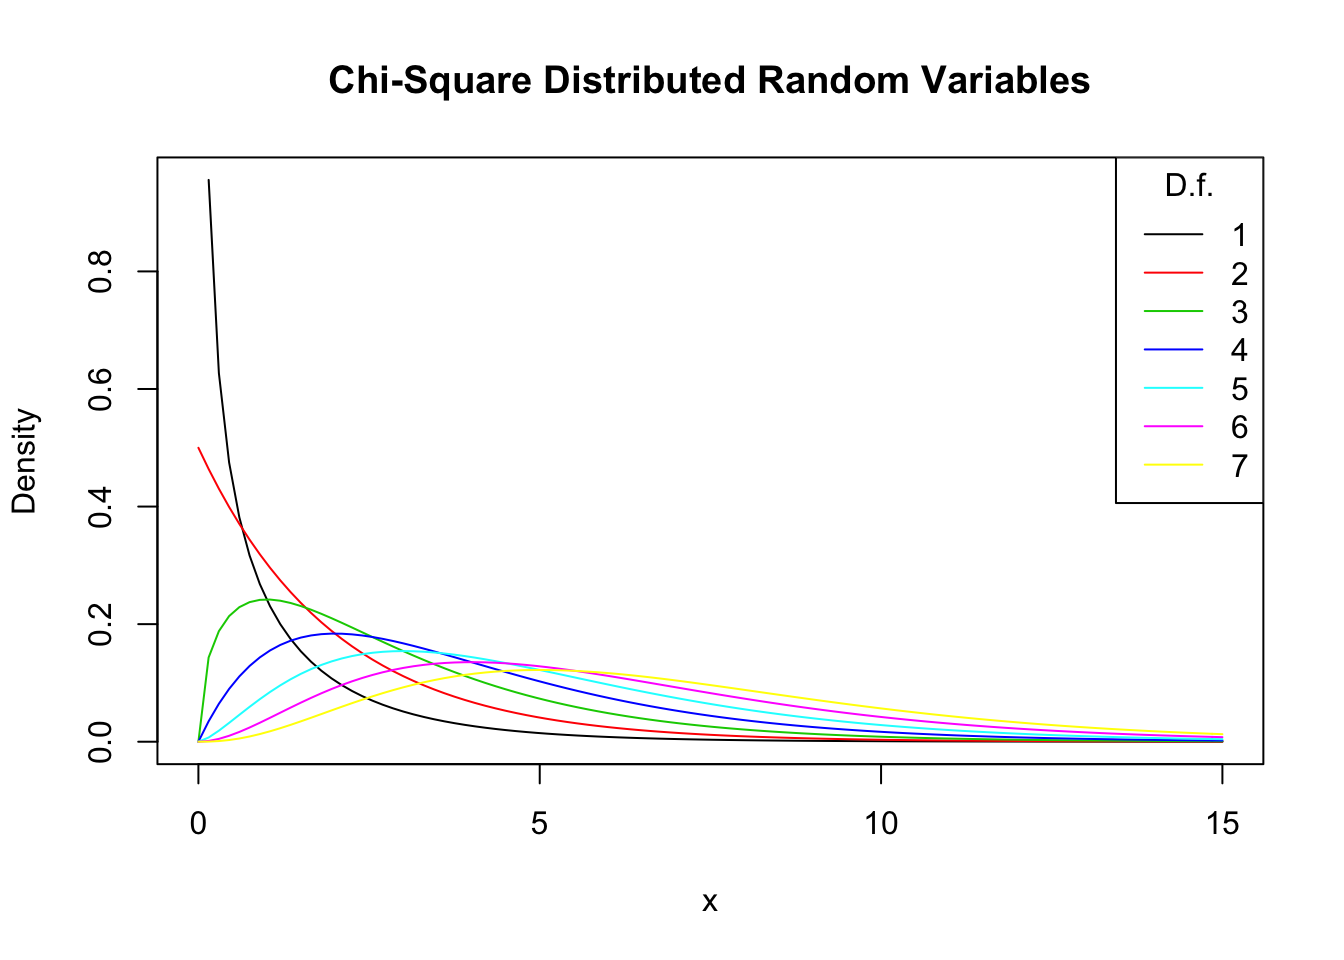
\includegraphics{URFITE_files/figure-latex/unnamed-chunk-28-1} \end{center}

It is evident that increasing the degrees of freedom shifts the
distribution to the right (the modus becomes larger) and increases its
dispersion (the distribution's variance grows).

\hypertarget{thetdist}{\subsection*{\texorpdfstring{The Student \(t\)
Distribution}{The Student t Distribution}}\label{thetdist}}
\addcontentsline{toc}{subsection}{The Student \(t\) Distribution}

Let \(Z\) be a standard normal variate, \(W\) a random variable that
follows a \(\chi^2_M\) distribution with \(M\) degrees of freedom and
further assume that \(Z\) and \(W\) are independently distributed. Then
it holds that

\[ \frac{Z}{\sqrt{W/M}} =:X \sim t_M \] and we say that \(X\) follows a
student \(t\) distribution (or simple \(t\) distribution) with \(M\)
degrees of freedom.

As for the \(\chi^2_M\) distribution, a \(t\) distribution depends on
the degrees of freedom \(M\). \(t\) distributions are symmetric,
bell-shaped and look very similar to a normal distribution, especially
when \(M\) is large. This is not a coincidence: for a sufficient large
\(M\), a \(t_M\) distribution can be approximated by the standard normal
distribution. This approximation works reasonably well for \(M\geq 30\).
As we will show later by means of a small simulation study, the
\(t_{\infty}\) distribution \emph{is} the standard normal distribution.

A \(t_M\) distributed random variable has an expectation value if
\(M>1\) and a variance if \(n>2\).

\begin{align}
  E(X) =& 0 \ , \ M>1 \\
  \text{Var}(X) =& \frac{M}{M-2} \ , \ M>2
\end{align}

Let us graph some \(t\) distributions with different \(M\) and compare
them with the standard normal distribution.

\begin{Shaded}
\begin{Highlighting}[]
\CommentTok{# plot the standard normal density}
\KeywordTok{curve}\NormalTok{(}\KeywordTok{dnorm}\NormalTok{(x), }
      \DataTypeTok{xlim=}\KeywordTok{c}\NormalTok{(}\OperatorTok{-}\DecValTok{4}\NormalTok{,}\DecValTok{4}\NormalTok{), }
      \DataTypeTok{xlab =} \StringTok{"x"}\NormalTok{, }
      \DataTypeTok{lty=}\DecValTok{2}\NormalTok{, }
      \DataTypeTok{ylab =} \StringTok{"Density"}\NormalTok{, }
      \DataTypeTok{main=}\StringTok{"Theoretical Densities of t-Distributions"}
\NormalTok{      )}

\CommentTok{# plot the t density for m=2}
\KeywordTok{curve}\NormalTok{(}\KeywordTok{dt}\NormalTok{(x, }\DataTypeTok{df=}\DecValTok{2}\NormalTok{), }
      \DataTypeTok{xlim=}\KeywordTok{c}\NormalTok{(}\OperatorTok{-}\DecValTok{4}\NormalTok{,}\DecValTok{4}\NormalTok{), }
      \DataTypeTok{col=}\DecValTok{2}\NormalTok{, }
      \DataTypeTok{add =}\NormalTok{ T}
\NormalTok{      )}

\CommentTok{# plot the t density for m=4}
\KeywordTok{curve}\NormalTok{(}\KeywordTok{dt}\NormalTok{(x, }\DataTypeTok{df=}\DecValTok{4}\NormalTok{), }
      \DataTypeTok{xlim=}\KeywordTok{c}\NormalTok{(}\OperatorTok{-}\DecValTok{4}\NormalTok{,}\DecValTok{4}\NormalTok{), }
      \DataTypeTok{col=}\DecValTok{3}\NormalTok{, }
      \DataTypeTok{add=}\NormalTok{T}
\NormalTok{      )}

\CommentTok{# plot the t density for m=25}
\KeywordTok{curve}\NormalTok{(}\KeywordTok{dt}\NormalTok{(x, }\DataTypeTok{df=}\DecValTok{25}\NormalTok{), }
      \DataTypeTok{xlim=}\KeywordTok{c}\NormalTok{(}\OperatorTok{-}\DecValTok{4}\NormalTok{,}\DecValTok{4}\NormalTok{), }
      \DataTypeTok{col=}\DecValTok{4}\NormalTok{, }
      \DataTypeTok{add=}\NormalTok{T}
\NormalTok{      )}

\CommentTok{# add a legend}
\KeywordTok{legend}\NormalTok{(}\StringTok{"topright"}\NormalTok{, }
       \KeywordTok{c}\NormalTok{(}\StringTok{"N(0,1)"}\NormalTok{,}\StringTok{"M=2"}\NormalTok{,}\StringTok{"M=4"}\NormalTok{,}\StringTok{"M=25"}\NormalTok{), }
       \DataTypeTok{col =} \DecValTok{1}\OperatorTok{:}\DecValTok{4}\NormalTok{, }
       \DataTypeTok{lty =} \KeywordTok{c}\NormalTok{(}\DecValTok{2}\NormalTok{,}\DecValTok{1}\NormalTok{,}\DecValTok{1}\NormalTok{,}\DecValTok{1}\NormalTok{)}
\NormalTok{       )}
\end{Highlighting}
\end{Shaded}

\begin{center}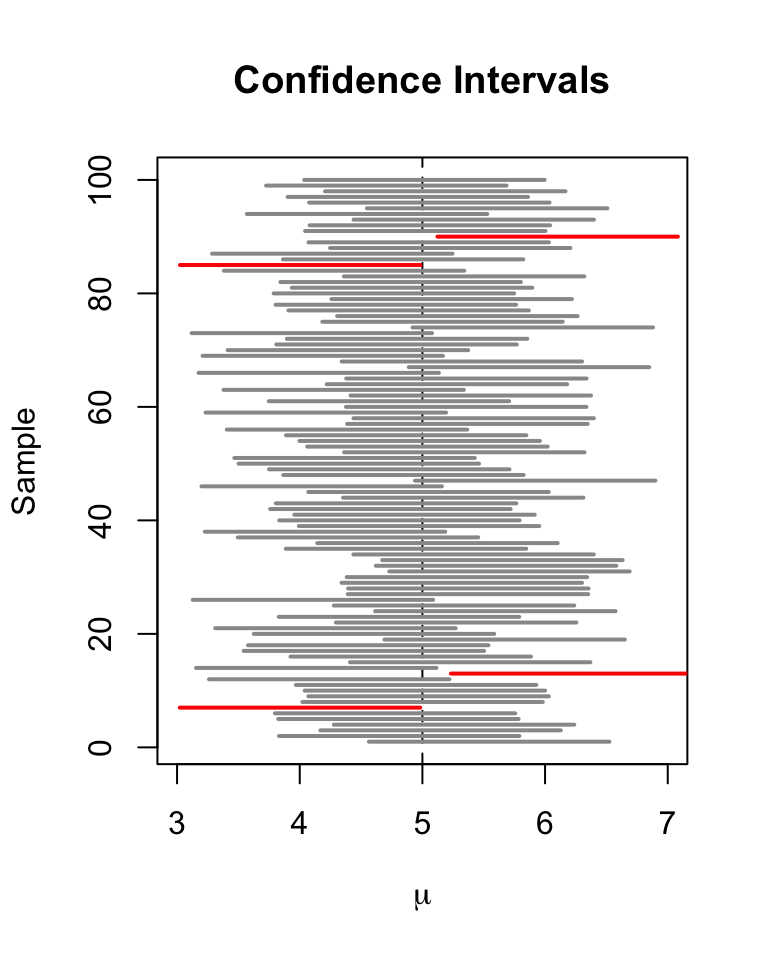
\includegraphics{URFITE_files/figure-latex/unnamed-chunk-29-1} \end{center}

The plot indicates what has been claimed in the previous paragraph: as
the degrees of freedom increase, the shape of the \(t\) distribution
comes closer to that of a standard normal bell. Already for \(M=25\) we
find little difference to the dashed line which belongs to the standard
normal density curve. If \(M\) is small, we find the distribution to
have slightly havier tails than a standard normal, i.e.~it has a
``fatter'' bell shape.

\subsection*{\texorpdfstring{The \(F\)
Distribution}{The F Distribution}}\label{the-f-distribution}
\addcontentsline{toc}{subsection}{The \(F\) Distribution}

Another ratio of random variables important to econometricians is the
ratio of two indpendently \(\chi^2\) distributed random variables that
are divided by their degrees of freedom. Such a quantity follows a \(F\)
distribution with numerator degrees of freedom \(M\) and denominator
degrees of freedom \(n\), denoted \(F_{M,n}\). The distribution was
first derived by George Snedecor but was named in honor of
\href{https://en.wikipedia.org/wiki/Ronald_Fisher}{Sir Ronald Fisher}.

\[ \frac{W/M}{V/n} \sim F_{M,n} \ \ \text{with} \ \ W \sim \chi^2_M \ \ , \ \ V \sim \chi^2_n \]

By definition, the domain of both PDF and CDF of a \(F_{M,n}\)
distributed random variable is \(\mathbb{R}_{\geq0}\).

Say we have a \(F\) distributed random variable \(Y\) with numerator
degrees of freedom \(3\) and denominator degrees of freedom \(14\) and
are interested in \(P(Y \geq 2)\). This can be computed with help of the
function \texttt{pf()}. By setting the argument \texttt{lower.tail} to
\texttt{TRUE} we ensure that R computes \(1- P(Y \leq 2)\), i.e.~the
probability mass in the tail right of \(2\).

\begin{Shaded}
\begin{Highlighting}[]
\KeywordTok{pf}\NormalTok{(}\DecValTok{2}\NormalTok{, }\DecValTok{3}\NormalTok{, }\DecValTok{13}\NormalTok{, }\DataTypeTok{lower.tail =}\NormalTok{ F)}
\end{Highlighting}
\end{Shaded}

\begin{verbatim}
## [1] 0.1638271
\end{verbatim}

We can visualize this probability by drawing a line plot of the related
density function and adding a color shading with \texttt{polygon()}.

\begin{Shaded}
\begin{Highlighting}[]
\CommentTok{# define coordinate vectors for vertices of the polygon}
\NormalTok{x <-}\StringTok{ }\KeywordTok{c}\NormalTok{(}\DecValTok{2}\NormalTok{, }\KeywordTok{seq}\NormalTok{(}\DecValTok{2}\NormalTok{, }\DecValTok{10}\NormalTok{, }\FloatTok{0.01}\NormalTok{), }\DecValTok{10}\NormalTok{)}
\NormalTok{y <-}\StringTok{ }\KeywordTok{c}\NormalTok{(}\DecValTok{0}\NormalTok{, }\KeywordTok{df}\NormalTok{(}\KeywordTok{seq}\NormalTok{(}\DecValTok{2}\NormalTok{, }\DecValTok{10}\NormalTok{, }\FloatTok{0.01}\NormalTok{), }\DecValTok{3}\NormalTok{, }\DecValTok{14}\NormalTok{), }\DecValTok{0}\NormalTok{)}

\CommentTok{# draw density of F_\{3, 14\}}
\KeywordTok{curve}\NormalTok{(}\KeywordTok{df}\NormalTok{(x ,}\DecValTok{3}\NormalTok{ ,}\DecValTok{14}\NormalTok{), }
      \DataTypeTok{ylim =} \KeywordTok{c}\NormalTok{(}\DecValTok{0}\NormalTok{, }\FloatTok{0.8}\NormalTok{), }
      \DataTypeTok{xlim =} \KeywordTok{c}\NormalTok{(}\DecValTok{0}\NormalTok{, }\DecValTok{10}\NormalTok{), }
      \DataTypeTok{ylab =} \StringTok{"Density"}\NormalTok{,}
      \DataTypeTok{main =} \StringTok{"Density Function"}
\NormalTok{      )}

\CommentTok{# draw the polygon}
\KeywordTok{polygon}\NormalTok{(x, y, }\DataTypeTok{col=}\StringTok{"orange"}\NormalTok{)}
\end{Highlighting}
\end{Shaded}

\begin{center}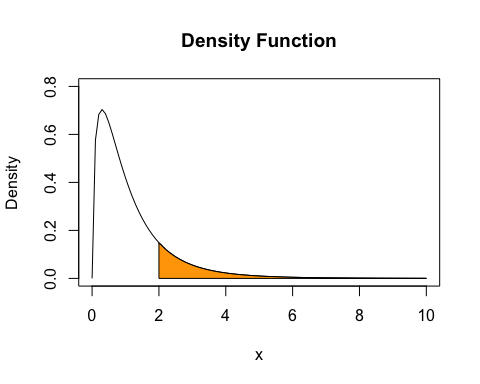
\includegraphics{URFITE_files/figure-latex/unnamed-chunk-31-1} \end{center}

The \(F\) distribution is related to many other distributions. An
important special case encountered in econometrics arises if the
denominator degrees of freedom are large such that the \(F_{M,n}\)
distribution can be approximated by the \(F_{M,\infty}\) distribution
which turns out to be simply the distribution of a \(\chi^2_M\) random
variable divided by its degrees of freedom \(M\).

\[ W/M \sim F_{M,\infty} \ \ , \ \ W \sim \chi^2_M \]

\section{Random Sampling and the Distribution of Sample
Averages}\label{random-sampling-and-the-distribution-of-sample-averages}

To clarify the basic idea of random sampling, let us jump back to the
die rolling example:

Suppose we are rolling the dice \(n\) times. This means we are
interested in the outcomes of \(n\) random processes
\(Y_i, \ i=1,...,n\) which are characterized by the same distribution.
Since these outcomes are selected randomly, they are \emph{random
variables} themselves and their realisations will differ each time we
draw a sample, i.e.~each time we roll the dice \(n\) times. Furthermore,
each observation is randomly drawn from the same population, that is the
numbers from \(1\) to \(6\), and their individual distribution is the
same. Hence we say that \(Y_1,\dots,Y_n\) are identically distributed.
Moreover, we know that the value of any of the \(Y_i\) does not provide
any information on the remainder of the sample. In our example, rolling
a six as the first observation in our sample does not alter the
distributions of \(Y_2,\dots,Y_n\): all numbers are equally likely to
occur. This means that all \(Y_i\) are also independently distributed.
Thus, we say that \(Y_1,\dots,Y_n\) are independently and identically
distributed (\emph{i.i.d}). The dice example is the simplest sampling
scheme used in statistics. That is why it is called \emph{simple random
sampling}. This concept is condensed in Key Concept 2.5.

Key Concept 2.5

Simple Random Sampling and i.i.d. Random Variables

In simple random sampling, \(n\) objects are drawn at random from a
population. Each object is equally likely to end up in the sample. We
denote the value of the random variable \(Y\) for the \(i^{th}\)
randomly drawn object as \(Y_i\). Since all objects are equally likely
to be drawn and the distribution of \(Y_i\) is the same for all \(i\),
the \(Y_i, \dots, Y_n\) are independently and identically distributed
(i.i.d.). This means the distribution of \(Y_i\) is the same for all
\(i=1,\dots,n\) and \(Y_1\) is distributed independently of
\(Y_2, \dots, Y_n\) \(Y_2\) is distributed independently of
\(Y_1, Y_3, \dots, Y_n\) and so forth.

What happens if we consider functions of the sample data? Consider the
example of rolling a dice two times in a row once again. A sample now
consists of two independent random draws from the set
\(\{1,2,3,4,5,6\}\). In view of the aforementioned, it is apparent that
any function of these two random variables is also random, e.g.~their
sum. Convince Yourself by executing the code below several times.

\begin{Shaded}
\begin{Highlighting}[]
\KeywordTok{sum}\NormalTok{(}\KeywordTok{sample}\NormalTok{(}\DecValTok{1}\OperatorTok{:}\DecValTok{6}\NormalTok{, }\DecValTok{2}\NormalTok{, }\DataTypeTok{replace =}\NormalTok{ T))}
\end{Highlighting}
\end{Shaded}

\begin{verbatim}
## [1] 6
\end{verbatim}

Clearly this sum, let us call it \(S\), is a random variable as it
depends on randomly drawn summands. For this example, we can completely
enumerate all outcomes and hence write down the theoretical probability
distribution of our function of the sample data, \(S\):

We face \(6^2=36\) possible pairs. Those pairs are

\begin{align}
  &(1,1)    (1,2)   (1,3)   (1,4)   (1,5)   (1,6) \\ 
  &(2,1)    (2,2)   (2,3)   (2,4)   (2,5)   (2,6) \\ 
  &(3,1)    (3,2)   (3,3)   (3,4)   (3,5)   (3,6) \\ 
  &(4,1)    (4,2)   (4,3)   (4,4)   (4,5)   (4,6) \\ 
  &(5,1)    (5,2)   (5,3)   (5,4)   (5,5)   (5,6) \\ 
  &(6,1)    (6,2)   (6,3)   (6,4)   (6,5)   (6,6)
\end{align}

Thus, possible outcomes for \(S\) are

\[ \left\{ 2,3,4,5,6,7,8,9,10,11,12 \right\} . \] Enumeration of
outcomes yields

\begin{align}
  P(S) = 
  \begin{cases} 
    1/36, \ & S = 2 \\ 
    2/36, \ & S = 3 \\
    3/36, \ & S = 4 \\
    4/36, \ & S = 5 \\
    5/36, \ & S = 6 \\
    6/36, \ & S = 7 \\
    5/36, \ & S = 8 \\
    4/36, \ & S = 9 \\
    3/36, \ & S = 10 \\
    2/36, \ & S = 11 \\
    1/36, \ & S = 12
  \end{cases}
\end{align}

We can also compute \(E(S)\) and \(\text{Var}(S)\) as stated in Key
Concept 2.1 and Key Concept 2.2.

\begin{Shaded}
\begin{Highlighting}[]
\CommentTok{# Vector of outcomes}
\NormalTok{S <-}\StringTok{ }\DecValTok{2}\OperatorTok{:}\DecValTok{12}

\CommentTok{# Vector of probabilities}
\NormalTok{PS <-}\StringTok{ }\KeywordTok{c}\NormalTok{(}\DecValTok{1}\OperatorTok{:}\DecValTok{6}\NormalTok{,}\DecValTok{5}\OperatorTok{:}\DecValTok{1}\NormalTok{)}\OperatorTok{/}\DecValTok{36}

\CommentTok{# Expectation of S}
\NormalTok{ES <-}\StringTok{ }\NormalTok{S }\OperatorTok\StringTok{ }\NormalTok{PS; ES}
\end{Highlighting}
\end{Shaded}

\begin{verbatim}
##      [,1]
## [1,]    7
\end{verbatim}

\begin{Shaded}
\begin{Highlighting}[]
\CommentTok{# Variance of S}
\NormalTok{VarS <-}\StringTok{ }\NormalTok{(S }\OperatorTok{-}\StringTok{ }\KeywordTok{c}\NormalTok{(ES))}\OperatorTok{^}\DecValTok{2} \OperatorTok\StringTok{ }\NormalTok{PS; VarS}
\end{Highlighting}
\end{Shaded}

\begin{verbatim}
##          [,1]
## [1,] 5.833333
\end{verbatim}

(The \texttt{\%*\%} operator is used to compute the scalar product of
two vectors.)

So the distribution of \(S\) is known. It is also evident that its
distribution differs considerably from the marginal distribution,
i.e.~the distribution of a single die roll's outcome, \(D\) . Let us
visualize this using barplots.

\begin{Shaded}
\begin{Highlighting}[]
\CommentTok{# divide the plotting area in one row with two columns}
\KeywordTok{par}\NormalTok{(}\DataTypeTok{mfrow =} \KeywordTok{c}\NormalTok{(}\DecValTok{1}\NormalTok{, }\DecValTok{2}\NormalTok{))}

\CommentTok{# plot the distribution of S}
\KeywordTok{names}\NormalTok{(PS) <-}\StringTok{ }\DecValTok{2}\OperatorTok{:}\DecValTok{12}

\KeywordTok{barplot}\NormalTok{(PS, }\DataTypeTok{ylim=}\KeywordTok{c}\NormalTok{(}\DecValTok{0}\NormalTok{,}\FloatTok{0.2}\NormalTok{), }
        \DataTypeTok{xlab =} \StringTok{"S"}\NormalTok{, }
        \DataTypeTok{ylab =}\StringTok{"Probability"}\NormalTok{, }
        \DataTypeTok{col=}\StringTok{"steelblue"}\NormalTok{, }
        \DataTypeTok{space=}\DecValTok{0}\NormalTok{, }
        \DataTypeTok{main=}\StringTok{"Sum of Two Die Rolls"}
\NormalTok{        )}

\CommentTok{# plot the distribution of D }
\NormalTok{probability <-}\StringTok{ }\KeywordTok{rep}\NormalTok{(}\DecValTok{1}\OperatorTok{/}\DecValTok{6}\NormalTok{,}\DecValTok{6}\NormalTok{)}
\KeywordTok{names}\NormalTok{(probability) <-}\StringTok{ }\DecValTok{1}\OperatorTok{:}\DecValTok{6}

\KeywordTok{barplot}\NormalTok{(probability, }
        \DataTypeTok{ylim=}\KeywordTok{c}\NormalTok{(}\DecValTok{0}\NormalTok{,}\FloatTok{0.2}\NormalTok{), }
        \DataTypeTok{xlab =} \StringTok{"D"}\NormalTok{, }
        \DataTypeTok{col=}\StringTok{"steelblue"}\NormalTok{, }
        \DataTypeTok{space =} \DecValTok{0}\NormalTok{, }
        \DataTypeTok{main =} \StringTok{"Outcome of a single Die Roll"}
\NormalTok{        )}
\end{Highlighting}
\end{Shaded}

\begin{center}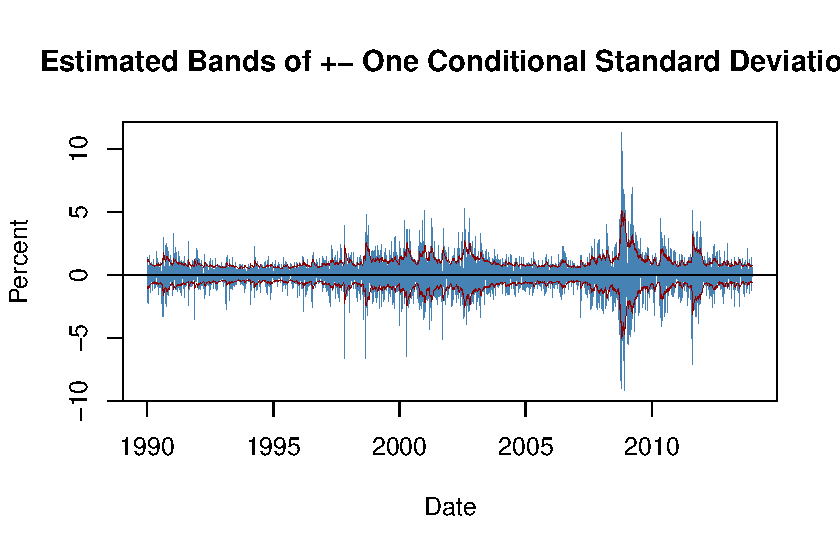
\includegraphics{URFITE_files/figure-latex/unnamed-chunk-34-1} \end{center}

Many econometric procedures deal with averages of sampled data. It is
almost always assumed that observations are drawn randomly from a
larger, unkown population. As demonstrated for the sample function
\(S\), computing an average of a random sample also has the effect to
make the average a random variable itself. This random variable in turn
has a probability distribution which is called the sampling
distribution. Knowledge about the sampling distribution of an average is
therefore crucial for understanding the performance of econometric
procedures.

The \emph{sample average} of a sample of \(n\) observations
\(Y_1, \dots, Y_n\) is

\[ \overline{Y} = \frac{1}{n} \sum_{i=1}^n Y_i = \frac{1}{n} (Y_1 + Y_2 + \cdots + Y_n). \]
\(\overline{Y}\) is also called the sample mean.

\subsection*{Mean and Variance of the Sample
Mean}\label{mean-and-variance-of-the-sample-mean}
\addcontentsline{toc}{subsection}{Mean and Variance of the Sample Mean}

Denote \(\mu_Y\) and \(\sigma_Y^2\) the mean and the variance of the
\(Y_i\) and suppose that all observations \(Y_1,\dots,Y_n\) are i.i.d.
such that in particular mean and variance are the same for all
\(i=1,\dots,n\). Then we have that

\[ E(\overline{Y}) = E\left(\frac{1}{n} \sum_{i=1}^n Y_i \right) = \frac{1}{n} E\left(\sum_{i=1}^n Y_i\right) = \frac{1}{n} \sum_{i=1}^n E\left(Y_i\right) = \frac{1}{n} \cdot n \cdot \mu_Y = \mu_Y    \]
and

\begin{align}
  \text{Var}(\overline{Y}) =& \text{Var}\left(\frac{1}{n} \sum_{i=1}^n Y_i \right) \\
  =& \frac{1}{n^2} \sum_{i=1}^n \text{Var}(Y_i) + \frac{1}{n^2} \sum_{i=1}^n \sum_{j=1, j\neq i}^n \text{cov}(Y_i,Y_j) \\
  =& \frac{\sigma^2_Y}{n} \\
  =& \sigma_{\overline{Y}}^2.
\end{align}

Note that the second summand vanishes since \(\text{cov}(Y_i,Y_j)=0\)
for \(i\neq j\) due to independence of the observations.

Consequently, the standard deviation of the sample mean is given by

\[ \sigma_{\overline{Y}} = \frac{\sigma_Y}{\sqrt{n}}. \]

It is worthwhile to mention that these results hold irrespective of the
underlying distribution of the \(Y_i\).

\subsubsection*{\texorpdfstring{The Sampling Distribution of
\(\overline{Y}\) when \(Y\) Is Normally
Distributed}{The Sampling Distribution of \textbackslash{}overline\{Y\} when Y Is Normally Distributed}}\label{the-sampling-distribution-of-overliney-when-y-is-normally-distributed}
\addcontentsline{toc}{subsubsection}{The Sampling Distribution of
\(\overline{Y}\) when \(Y\) Is Normally Distributed}

If the \(Y_1,\dots,Y_n\) are i.i.d. draws from a normal distribution
with mean \(\mu_Y\) and variance \(\sigma_Y^2\), the following holds for
their sample average \(\overline{Y}\):

\[ \overline{Y} \sim N(\mu_y, \sigma_Y^2/n) \tag{2.4} \]

For example, if a sample \(Y_i\) with \(i=1,\dots,10\) is drawn from a
standard normal distribution with mean \(\mu_Y = 0\) and variance
\(\sigma_Y^2=1\) we have

\[ \overline{Y} \sim N(0,0.1).\]

We can use R's random number generation facilities to verifiy this
result. The basic idea is to simulate outcomes of the true distribution
of \(\overline{Y}\) by repeatedly drawing random samples of 10
observation from the \(N(0,1)\) distribution and computing their
respective averages. If we do this for a large number of repititions,
the simulated dataset of averages should quite accurately reflect the
theoretical distribution of \(\overline{Y}\) if the theoretical result
holds.

The approach sketched above is an example of what is commonly known as
\emph{Monte Carlo Simulation} or \emph{Monte Carlo Experiment}. To
perform this simulation in R, we proceed as follows:

\begin{enumerate}
\def\labelenumi{\arabic{enumi}.}
\tightlist
\item
  Choose a sample size \texttt{n} and the number of samples to be drawn
  \texttt{reps}.
\item
  Use the function \texttt{replicate()} in conjunction with
  \texttt{rnorm()} to draw \texttt{n} observations from the standard
  normal distribution \texttt{rep} times. \textbf{Note}: the outcome of
  \texttt{replicate()} is a matrix with dimensions \texttt{n} \(\times\)
  \texttt{rep}. It contains the drawn samples as \emph{columns}.
\item
  Compute sample means using \texttt{colMeans()}. This function computes
  the mean of each column i.e.~of each sample and returns a vector.
\end{enumerate}

\begin{Shaded}
\begin{Highlighting}[]
\CommentTok{# Set sample size and number of samples}
\NormalTok{n <-}\StringTok{ }\DecValTok{10}
\NormalTok{reps <-}\StringTok{ }\DecValTok{10000}

\CommentTok{# Perform random sampling}
\NormalTok{samples <-}\StringTok{ }\KeywordTok{replicate}\NormalTok{(reps, }\KeywordTok{rnorm}\NormalTok{(n)) }\CommentTok{# 10 x 10000 sample matrix}

\CommentTok{# Compute sample means}
\NormalTok{sample.avgs <-}\StringTok{ }\KeywordTok{colMeans}\NormalTok{(samples)}
\end{Highlighting}
\end{Shaded}

After performing these steps we end up with a vector of sample averages.
You can check the vector property of \texttt{sample.avgs}:

\begin{Shaded}
\begin{Highlighting}[]
\CommentTok{# Check that sample.avgs is a vector}
\KeywordTok{is.vector}\NormalTok{(sample.avgs) }
\end{Highlighting}
\end{Shaded}

\begin{verbatim}
## [1] TRUE
\end{verbatim}

\begin{Shaded}
\begin{Highlighting}[]
\CommentTok{# print the first few entries to the console}
\KeywordTok{head}\NormalTok{(sample.avgs)}
\end{Highlighting}
\end{Shaded}

\begin{verbatim}
## [1] -0.12406767 -0.10649421 -0.01033423 -0.39905236 -0.41897968 -0.90883537
\end{verbatim}

A straightforward approach to examine the distribution of univariate
numerical data is to plot it as a histogram and compare it to some known
or assumed distribution. This comparison can be done with help of a
suitable statistical test or by simply eyeballing some graphical
representations of these distributions. For our simulated sample
averages, we will do the latter by means of the functions
\texttt{hist()} and \texttt{curve()}.

By default, \texttt{hist()} will give us a frequency histogram i.e.~a
bar chart where observations are grouped into ranges, also called bins.
The ordinate reports the number of observations falling into each of the
bins. Instead, we want it to report density estimates for comparison
purposes. This is achieved by setting the argument
\texttt{freq\ =\ FALSE}. The number of bins is adjusted by the argument
\texttt{breaks}.

Using \texttt{curve()}, we overlay the histogram with a red line which
represents the theoretical density of a \(N(0, 0.1)\) distributed random
variable. Remember to use the argument \texttt{add\ =\ TRUE} to add the
curve to the current plot. Otherwise R will open a new graphic device
and discard the histogram plot!

\begin{Shaded}
\begin{Highlighting}[]
\CommentTok{# Plot the density histogram}
\KeywordTok{hist}\NormalTok{(sample.avgs, }
     \DataTypeTok{ylim=}\KeywordTok{c}\NormalTok{(}\DecValTok{0}\NormalTok{,}\FloatTok{1.4}\NormalTok{), }
     \DataTypeTok{col=}\StringTok{"steelblue"}\NormalTok{ , }
     \DataTypeTok{freq =}\NormalTok{ F, }
     \DataTypeTok{breaks =} \DecValTok{20}
\NormalTok{     )}

\CommentTok{# overlay the theoretical distribution of sample averages on top of the histogram}
\KeywordTok{curve}\NormalTok{(}\KeywordTok{dnorm}\NormalTok{(x, }\DataTypeTok{sd =} \DecValTok{1}\OperatorTok{/}\KeywordTok{sqrt}\NormalTok{(n)), }
      \DataTypeTok{col=}\StringTok{"red"}\NormalTok{, }
      \DataTypeTok{lwd=}\StringTok{"2"}\NormalTok{, }
      \DataTypeTok{add=}\NormalTok{T}
\NormalTok{      )}
\end{Highlighting}
\end{Shaded}

\begin{center}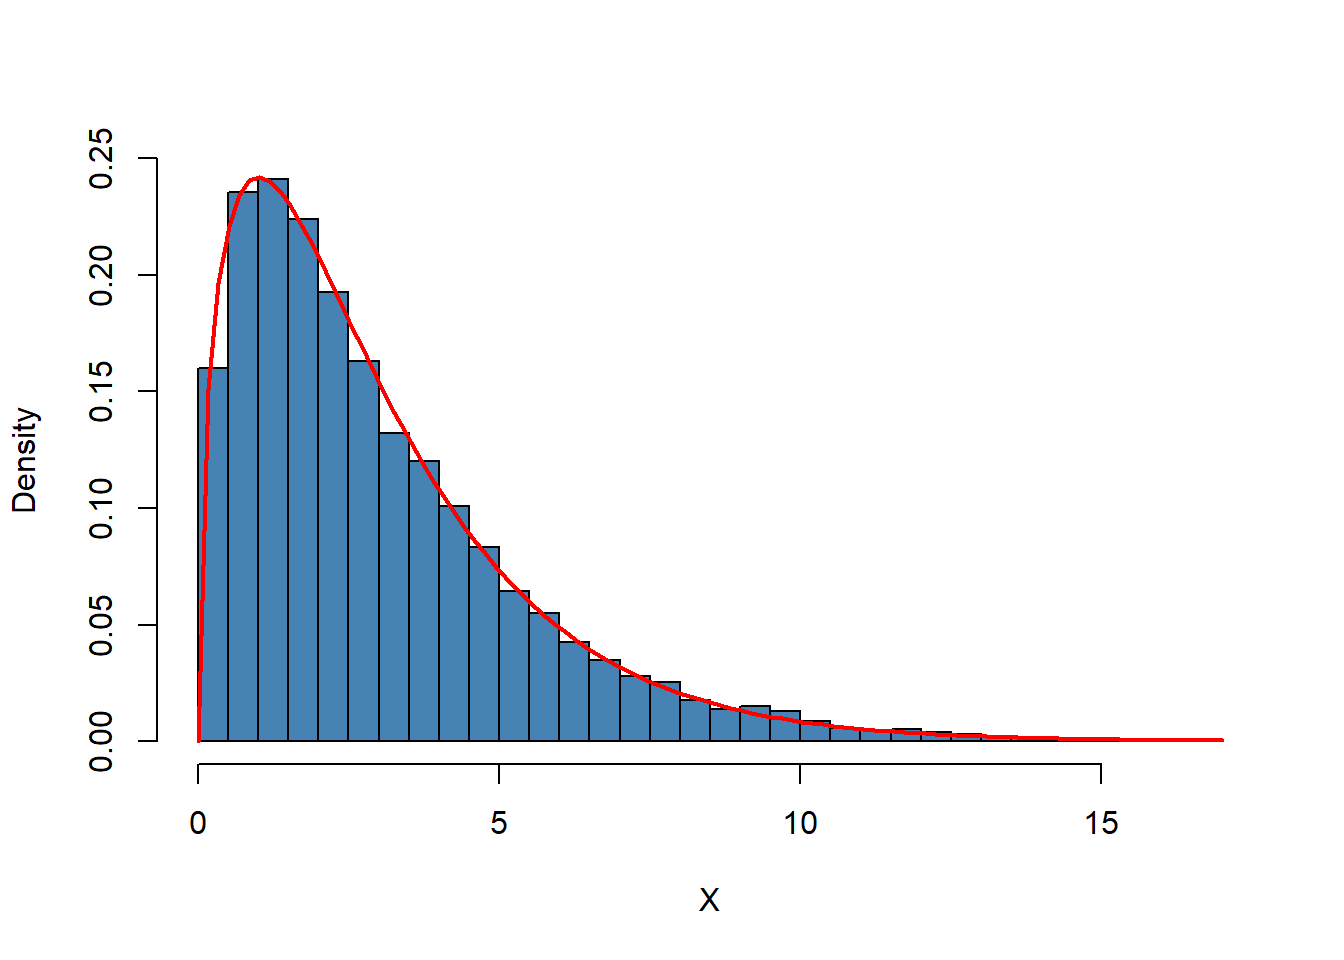
\includegraphics{URFITE_files/figure-latex/unnamed-chunk-37-1} \end{center}

From inspection of the plot we can tell that the distribution of
\(\overline{Y}\) is indeed very close to that of a \(N(0, 0.1)\)
distributed random variable so that evidence obained from the Monte
Carlo Simulation supports the theoretical claim.

Let us discuss another example where using simple random sampling in a
simulation setup helps to verify a well known result. As discussed
before, the \protect\hyperlink{chisquare}{Chi-squared} distribution with
\(m\) degrees of freedom arises as the distribution of the sum of \(m\)
independent squared standard normal distributed random variables.

To visualize the claim stated in equation (2.3), we proceed similarly as
in the example before:

\begin{enumerate}
\def\labelenumi{\arabic{enumi}.}
\tightlist
\item
  Choose the degrees of freedom \texttt{DF} and the number of samples to
  be drawn \texttt{reps}.
\item
  Draw \texttt{reps} random samples of size \texttt{DF} from the
  standard normal distribution using \texttt{replicate()}.
\item
  For each sample, by squaring the outcomes and summing them up
  columnwise. Store the results
\end{enumerate}

Again, we produce a density estimate for the distribution underlying our
simulated data using a density histogram and overlay it with a line
graph of the theoretical density function of the \(\chi^2_3\)
distribution.

\begin{Shaded}
\begin{Highlighting}[]
\CommentTok{# Number of repititions}
\NormalTok{reps <-}\StringTok{ }\DecValTok{10000}

\CommentTok{# Set degrees of freedom of a chi-Square Distribution}
\NormalTok{DF <-}\StringTok{ }\DecValTok{3} 

\CommentTok{# Sample 10000 column vectors à 3 N(0,1) R.V.S}
\NormalTok{Z <-}\StringTok{ }\KeywordTok{replicate}\NormalTok{(reps, }\KeywordTok{rnorm}\NormalTok{(DF)) }

\CommentTok{# Column sums of squares}
\NormalTok{X <-}\StringTok{ }\KeywordTok{colSums}\NormalTok{(Z}\OperatorTok{^}\DecValTok{2}\NormalTok{)}

\CommentTok{# Histogram of column sums of squares}
\KeywordTok{hist}\NormalTok{(X, }
     \DataTypeTok{freq =}\NormalTok{ F, }
     \DataTypeTok{col=}\StringTok{"steelblue"}\NormalTok{, }
     \DataTypeTok{breaks =} \DecValTok{40}\NormalTok{, }
     \DataTypeTok{ylab=}\StringTok{"Density"}\NormalTok{, }
     \DataTypeTok{main=}\StringTok{""}
\NormalTok{     )}

\CommentTok{# Add theoretical density}
\KeywordTok{curve}\NormalTok{(}\KeywordTok{dchisq}\NormalTok{(x, }\DataTypeTok{df =}\NormalTok{ DF), }
      \DataTypeTok{type =} \StringTok{'l'}\NormalTok{, }
      \DataTypeTok{lwd =} \DecValTok{2}\NormalTok{, }
      \DataTypeTok{col=}\StringTok{"red"}\NormalTok{, }
      \DataTypeTok{add =}\NormalTok{ T}
\NormalTok{      )}
\end{Highlighting}
\end{Shaded}

\begin{center}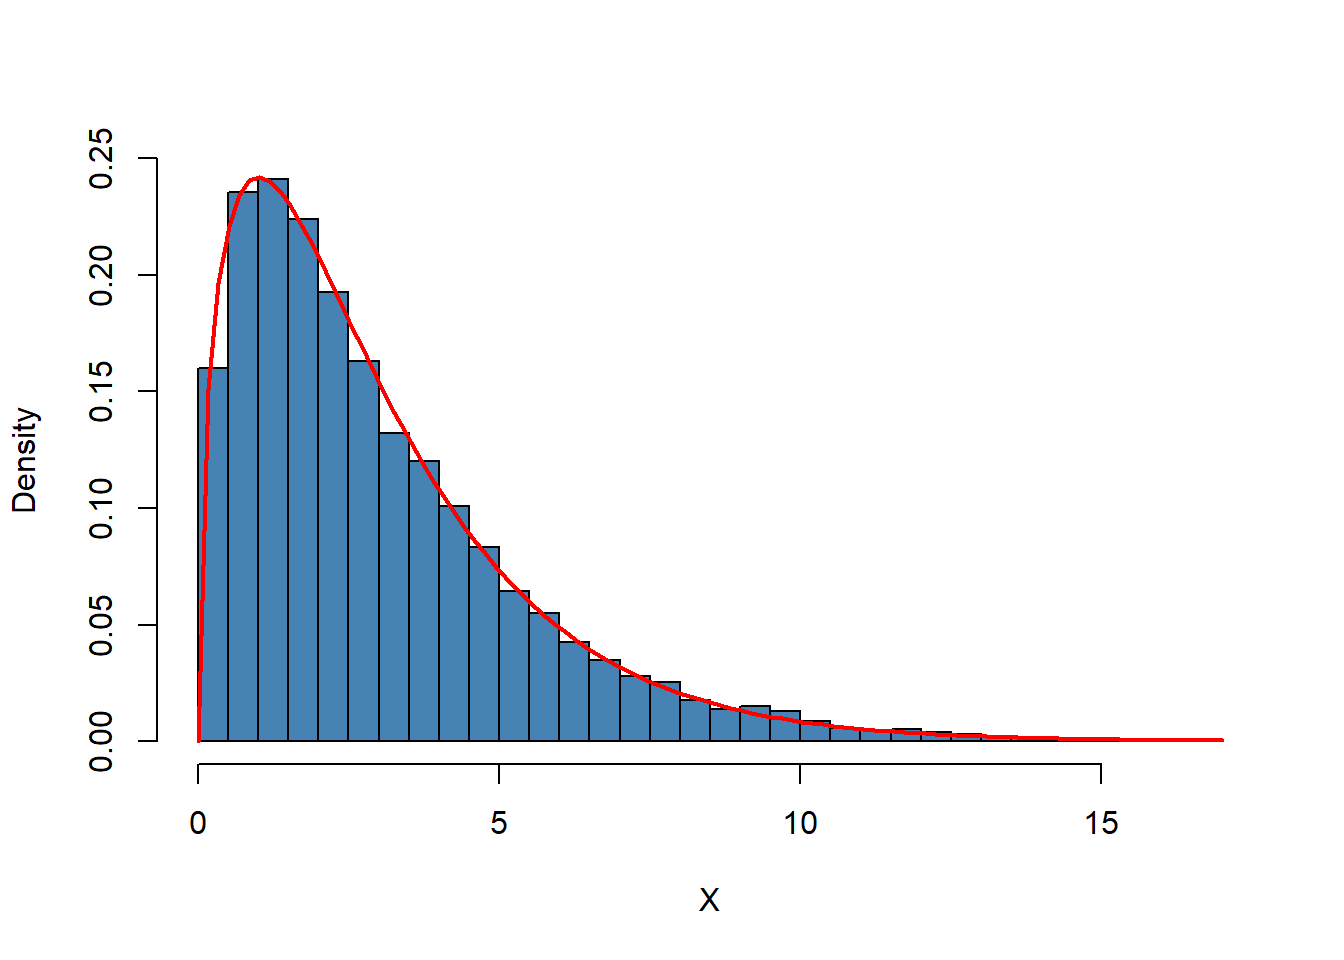
\includegraphics{URFITE_files/figure-latex/unnamed-chunk-38-1} \end{center}

\subsection*{Large Sample Approximations to Sampling
Distributions}\label{large-sample-approximations-to-sampling-distributions}
\addcontentsline{toc}{subsection}{Large Sample Approximations to
Sampling Distributions}

Sampling distributions as considered in the last section play an
important role in the development of econometric methods. In general,
there are two different approaches in characterizing sampling
distributions: an ``exact'' approach and an ``approximate'' approach.

The exact approach aims to find a general formula for the sampling
distribution that holds for any sample size \(n\). We call this the
\emph{exact distribution} or \emph{finite sample distribution}. In the
previous examples of die rolling and normal variates, we have dealt with
functionals of random variables whose sample distributions are
\emph{excactly known} in the sense that we can write them down as
analytical expressions and do calculations. However, this is not always
possible. For \(\overline{Y}\), result (2.4) tells us that normality of
the \(Y_i\) implies normality of \(\overline{Y}\) (we demonstrated this
for the special case of \(Y_i \overset{i.i.d.}{\sim} N(0,1)\) with
\(n=10\) using a simulation study that involves random sampling).
Unfortunately, the \emph{exact} distribution of \(\overline{Y}\) is
unknown, very hard to derive or even untractable if we drop the
assumption of \(Y\) having a normal distribution.

Therefore, as can be guessed from its name, the ``approximate'' approach
aims to find an approximation to the sampling distribution wherby it is
required that the sample size \(n\) is large. A distribution that is
used as a large-sample approximation to the sampling distribution is
also called the \emph{asymptotic distribution}. This is due to the fact
that the asymptotic distribution \emph{is} the sampling distribution for
\(n \rightarrow \infty\) i.e.~the approximation becomes exact if the
sample size goes to infinity. However, there are cases where the
difference between the sampling distribution and the asymptotic
distribution is negligible for moderate or even small samples sizes so
that approximations work very good.

In this section we will discuss two well known results that are used to
approximate sampling distributions and thus consitute key tools in
econoemtric theory: the \emph{law of large numbers} and the
\emph{central limit theorem}. The law of large numbers states that in
large samples, \(\overline{Y}\) is close to \(\mu_Y\) with high
probability. The central limit theorem says that the sampling
distribution of the standardized sample average, that is
\((\overline{Y} - \mu_Y)/\sigma_{\overline{Y}}\) is asymptotically
normal distributed. It is particualarly interesting that both results do
not depend on the distribution of \(Y\). In other words, beeing unable
to describe the complicated sampling distribution of \(\overline{Y}\) if
\(Y\) is not normal, approximations of the latter using the central
limit theorem simplify the development and applicability of econometric
procedures enormously. This is a key component underlying the theory of
statistical inference for regression models. Both results are summarized
in Key Concept 2.6 and Key Concept 2.7.

Key Concept 2.6

Convergence in Probability, Consistency and the Law of Large Numbers

The sample average \(\overline{Y}\) converges in probability to
\(\mu_Y\) --- we say that \(\overline{Y}\) is \emph{consistent} for
\(\mu_Y\) --- if the probability that \(\overline{Y}\) is in the range
\((\mu_Y - \epsilon)\) to \((\mu_Y + \epsilon)\) becomes arbitrarly
close to \(1\) as \(n\) increases for any constant \(\epsilon > 0\). We
write this short as

\[ \overline{Y} \xrightarrow[]{p} \mu_Y. \]

Consider the independently and identically distributed random variables
\(Y_i, i=1,\dots,n\) with expectation \(E(Y_i)=\mu_Y\) and variance
\(\text{Var}(Y_i)=\sigma^2_Y\). Under the condition that
\(\sigma^2_Y< \infty\), that is large outliers are unlikely, the law of
large numbers states

\[ \overline{Y} \xrightarrow[]{p} \mu_Y. \]

The core statement of the law of large numbers is that under quite
general conditions, the probability of obtaining a sample average
\(\overline{Y}\) that is close to \(\mu_Y\) is high if we have a large
sample size.

Consider the example of repeatedly tossing a coin where \(Y_i\) is the
result of the \(i^{th}\) coin toss. \(Y_i\) is a Bernoulli distributed
random variable with

\[ P(Y_i) = \begin{cases} p, & Y_i = 1 \\ 1-p, & Y_i = 0 \end{cases} \]
where \(p = 0.5\) as we assume a fair coin. It is straightforward to
show that

\[ \mu_Y = p = 0.5. \] Say \(p\) is the probabiliy of observing head and
denote \(R_n\) the proportion of heads in the first \(n\) tosses,

\[ R_n = \frac{1}{n} \sum_{i=1}^n Y_i. \tag{2.5}\]

According to the law of large numbers, the observed proportion of heads
converges in probability to \(\mu_Y = 0.5\), the probability of tossing
head in a single coin toss,

\[ R_n \xrightarrow[]{p} \mu_Y=0.5 \ \ \text{as} \ \ n \rightarrow \infty.  \]
The following application simulates \(1000\) coin tosses with a fair
coin and computes the fraction of heads observed for each additional
toss interactively. The result is a random path that, as stated by the
law of large numbers, shows a tendency to approach the vaule of \(0.5\)
as \(n\) grows.

We can use R to compute and illustrate such paths by simulation. The
procedure is as follows:

\begin{enumerate}
\def\labelenumi{\arabic{enumi}.}
\tightlist
\item
  Sample \texttt{N} observations from the Bernoulli distribution
  e.g.~using \texttt{sample()}.
\item
  Calculate the proportion of heads \(R_n\) as in (2.5). A way to
  achieve this is to call \texttt{cumsum()} on the vector of
  observations \texttt{Y} to obtain its cumulative sum and then divide
  by the respective number of observations.
\end{enumerate}

We continue by plotting the path and also add a dashed line for the
benchmark \(R_n = p = 0.5\).

\begin{Shaded}
\begin{Highlighting}[]
\CommentTok{# set random seed}
\KeywordTok{set.seed}\NormalTok{(}\DecValTok{1}\NormalTok{)}

\CommentTok{# Set number of coin tosses and simulate}
\NormalTok{N <-}\StringTok{ }\DecValTok{30000}
\NormalTok{Y <-}\StringTok{ }\KeywordTok{sample}\NormalTok{(}\DecValTok{0}\OperatorTok{:}\DecValTok{1}\NormalTok{, N, }\DataTypeTok{replace =}\NormalTok{T)}

\CommentTok{# Calculate R_n for 1:N}
\NormalTok{S <-}\StringTok{ }\KeywordTok{cumsum}\NormalTok{(Y)}
\NormalTok{R <-}\StringTok{ }\NormalTok{S}\OperatorTok{/}\NormalTok{(}\DecValTok{1}\OperatorTok{:}\NormalTok{N)}

\CommentTok{# Plot the path.}
\KeywordTok{plot}\NormalTok{(R, }
     \DataTypeTok{ylim=}\KeywordTok{c}\NormalTok{(}\FloatTok{0.3}\NormalTok{, }\FloatTok{0.7}\NormalTok{), }
     \DataTypeTok{type =} \StringTok{"l"}\NormalTok{, }
     \DataTypeTok{col =} \StringTok{"steelblue"}\NormalTok{, }
     \DataTypeTok{lwd =} \DecValTok{2}\NormalTok{, }
     \DataTypeTok{xlab =} \StringTok{"n"}\NormalTok{, }
     \DataTypeTok{ylab =} \StringTok{"R_n"}\NormalTok{,}
     \DataTypeTok{main =} \StringTok{"Converging Share of Heads in Repeated Coin Tossing"}
\NormalTok{     )}

\CommentTok{# Add a dashed line for R_n = 0.5}
\KeywordTok{lines}\NormalTok{(}\KeywordTok{c}\NormalTok{(}\DecValTok{0}\NormalTok{,N), }
      \KeywordTok{c}\NormalTok{(}\FloatTok{0.5}\NormalTok{, }\FloatTok{0.5}\NormalTok{), }
      \DataTypeTok{col =} \StringTok{"darkred"}\NormalTok{, }
      \DataTypeTok{lty =} \DecValTok{2}\NormalTok{, }
      \DataTypeTok{lwd =} \DecValTok{1}
\NormalTok{      )}
\end{Highlighting}
\end{Shaded}

\begin{center}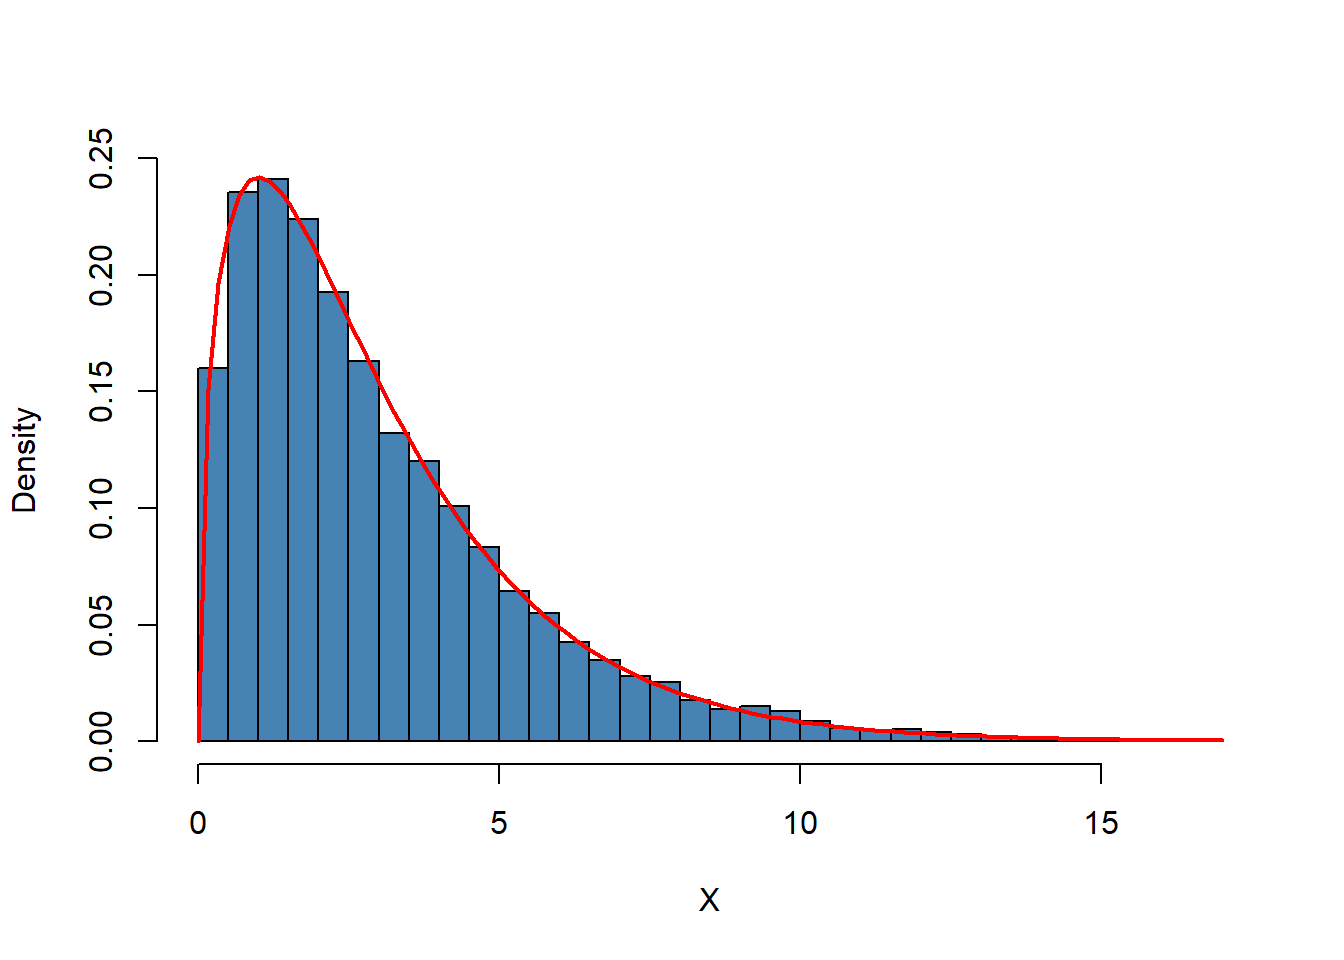
\includegraphics{URFITE_files/figure-latex/unnamed-chunk-39-1} \end{center}

There are several things to be said about this plot.

\begin{itemize}
\item
  The blue graph shows the observed proportion of heads when tossing a
  coin \(n\) times.
\item
  Since the \(Y_i\) are radnom variables, \(R_n\) is a random variate,
  too. The path depicted is only one of many possible realisations of
  \(R_n\) as it is determined by the \(30000\) observations sampled from
  the Bernoulli distribution. Thus, the code chunk above produces a
  differnt path every time You execute it (try this!).
\item
  If the number of coin tosses \(n\) is small, we observe the proportion
  of heads to be anything but close to its theoretical value,
  \(\mu_Y = 0.5\). However, as more and more observation are included in
  the sample we find that the path stabilizes in neighbourhood of
  \(0.5\). This is the message to take away: the average of multiple
  trials shows a clear tendency to converge to its expected value as the
  sample size increases, just as claimed by the law of large numbers.
\end{itemize}

Key Concept 2.6

The Central Limit Theorem

Suppose that \(Y_1,\dots,Y_n\) are independently and identically
distributed random variables with expectation \(E(Y_i)=\mu_Y\) and
variance \(\text{Var}(Y_i)=\sigma^2_Y\), \(0<\sigma^2_Y<\infty\). The
central limit theorem states that, if the sample size \(n\) goes to
infinity, the distribution of the scaled (by \(\sqrt{n}\)) standardized
sample average
\[ \frac{\overline{Y} - \mu_Y}{\sigma_{\overline{Y}}} = \frac{\overline{Y} - \mu_Y}{\sigma_Y/\sqrt{n}} \ \]
becomes arbitrarily well approximated by the standard normal
distribution.

According to the central limit theorem, the distribution of the sample
mean \(\overline{Y}\) of the bernoulli distributed random variables
\(Y_i\), \(i=1,...,n\) is well approximated by the normal distribution
with parameters \(\mu_Y=p=0.5\) and
\(\sigma^2_{\overline{Y}} = p(1-p) = 0.25\) for large \(n\).
Consequently, for the standardized sample mean we conclude that the
ratio

\[ \frac{\overline{Y} - 0.5}{0.5/\sqrt{n}} \tag{2.6}\] should be well
approximated by the standard normal distribution \(N(0,1)\). We employ
another simulation study to demonstrate this graphically. The idea is as
follows.

Draw a large number of random samples, \(10000\) say, of size \(n\) from
the Bernoulli distribution and compute the sample averages. Standardize
the averages as shown in (2.6). Next, visualize the distribution of the
generated standardized sample averages by means of a density histogram
and compare to the standard normal distribution. Repeat this for
different sample sizes \(n\) to see how increasing the sample size \(n\)
impacts the simulated distribution of the averages.

In R, we realized this as follows:

\begin{enumerate}
\def\labelenumi{\arabic{enumi}.}
\item
  We start by defining that the next four subsequently generated figures
  shall be drawn in a \(2\times2\) array such that they can be easily
  compared. This is done by calling \texttt{par(mfrow\ =\ c(2,\ 2))}
  before the figures are generated.
\item
  We define the number of repetitions \texttt{reps} as \(10000\) and
  create a vector of sample sizes named \texttt{sample.sizes}. We
  consider samples of sizes \(2\), \(10\), \(50\) and \(100\).
\item
  Next, we combine two \texttt{for()} loops to simulate the data and
  plot the distributions. The inner loop generates \(10000\) random
  samples, each consisting of \texttt{n} observations that are drawn
  from the bernoulli distribution, and computes the standardized
  averages. The outer loop executes the inner loop for the different
  sample sizes \texttt{n} and produces a plot for each iteration.
\end{enumerate}

\begin{Shaded}
\begin{Highlighting}[]
\CommentTok{# Subdivide the plot panel into a 2-by-2 array}
\KeywordTok{par}\NormalTok{(}\DataTypeTok{mfrow =} \KeywordTok{c}\NormalTok{(}\DecValTok{2}\NormalTok{, }\DecValTok{2}\NormalTok{))}

\CommentTok{# Set number of repetitions and the sample sizes}
\NormalTok{reps <-}\StringTok{ }\DecValTok{10000}
\NormalTok{sample.sizes <-}\StringTok{ }\KeywordTok{c}\NormalTok{(}\DecValTok{2}\NormalTok{, }\DecValTok{10}\NormalTok{, }\DecValTok{50}\NormalTok{, }\DecValTok{100}\NormalTok{)}

\CommentTok{# outer loop (loop over the sample sizes)}
  \ControlFlowTok{for}\NormalTok{ (n }\ControlFlowTok{in}\NormalTok{ sample.sizes) \{}
    
\NormalTok{    samplemean <-}\StringTok{ }\KeywordTok{rep}\NormalTok{(}\DecValTok{0}\NormalTok{,reps) }\CommentTok{#initialize the vector of sample menas}
\NormalTok{    stdsamplemean <-}\StringTok{ }\KeywordTok{rep}\NormalTok{(}\DecValTok{0}\NormalTok{,reps) }\CommentTok{#initialize the vector of standardized sample menas}

\CommentTok{# inner loop (loop over repetitions)   }
    \ControlFlowTok{for}\NormalTok{ (i }\ControlFlowTok{in} \DecValTok{1}\OperatorTok{:}\NormalTok{reps) \{}
\NormalTok{      x <-}\StringTok{ }\KeywordTok{rbinom}\NormalTok{(n,}\DecValTok{1}\NormalTok{,}\FloatTok{0.5}\NormalTok{)}
\NormalTok{      samplemean[i] <-}\StringTok{ }\KeywordTok{mean}\NormalTok{(x)}
\NormalTok{      stdsamplemean[i] <-}\StringTok{ }\KeywordTok{sqrt}\NormalTok{(n)}\OperatorTok{*}\NormalTok{(}\KeywordTok{mean}\NormalTok{(x)}\OperatorTok{-}\FloatTok{0.5}\NormalTok{)}\OperatorTok{/}\FloatTok{0.5}
\NormalTok{    \}}
    
\CommentTok{# plot the histogram and overlay it with the N(0,1) density for every iteration    }
    \KeywordTok{hist}\NormalTok{(stdsamplemean, }
         \DataTypeTok{col =} \StringTok{"steelblue"}\NormalTok{, }
         \DataTypeTok{breaks =} \DecValTok{40}\NormalTok{, }
         \DataTypeTok{freq =} \OtherTok{FALSE}\NormalTok{, }
         \DataTypeTok{xlim=}\KeywordTok{c}\NormalTok{(}\OperatorTok{-}\DecValTok{3}\NormalTok{, }\DecValTok{3}\NormalTok{), }
         \DataTypeTok{ylim =} \KeywordTok{c}\NormalTok{(}\DecValTok{0}\NormalTok{, }\FloatTok{0.4}\NormalTok{), }
         \DataTypeTok{xlab =} \KeywordTok{paste}\NormalTok{(}\StringTok{"n ="}\NormalTok{, n), }
         \DataTypeTok{main =} \StringTok{""}
\NormalTok{         )}
    
    \KeywordTok{curve}\NormalTok{(}\KeywordTok{dnorm}\NormalTok{(x), }
          \DataTypeTok{lwd =} \DecValTok{2}\NormalTok{, }
          \DataTypeTok{col=}\StringTok{"darkred"}\NormalTok{, }
          \DataTypeTok{add =} \OtherTok{TRUE}
\NormalTok{          )}
\NormalTok{  \}  }
\end{Highlighting}
\end{Shaded}

\begin{center}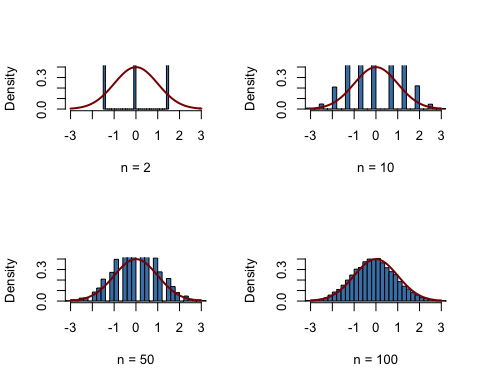
\includegraphics{URFITE_files/figure-latex/unnamed-chunk-40-1} \end{center}

We see that the simulated sampling distribution of the standardized
average tends to deviate strongly from the standard normal distribution
if the sample size is small, e.g.~for \(n=5\) and \(n=10\). However as
\(n\) grows, the histograms are approaching the bell shape of a standard
normal and we can be confident that the approximation works quite well
as seen for \(n=100\).

\chapter{A Review of Statistics using
R}\label{a-review-of-statistics-using-r}

This section reviews important statistical concepts:

\begin{itemize}
\item
  Estimation
\item
  Hypothesis testing
\item
  Confidence intervals
\end{itemize}

Since these types of statistical methods are heavily used in
econometrics, we will discuss them in the context of inference about an
unknown population mean and discuss several applications in R.

\section{Estimation of the Population
Mean}\label{estimation-of-the-population-mean}

Key Concept 3.1

Estimators and Estimates

Estimators are functions of sample data that are drawn randomly from an
unknown population. Estimates are numerical values computed by
estimators based on the sample data. Estimators are random variables
because they are functions of \emph{random} data. Estimates are
nonrandom numbers.

Think of some economic variable, for example hourly earnings of college
graduates, denoted by \(Y\). Suppose we are interested in \(\mu_Y\) the
mean of \(Y\). In order to exactly calculate \(\mu_Y\) we would have to
interview every graduated member of the working population in the
economy. We simply cannot do this for time and cost reasons. However, we
could draw a random sample from \(n\) i.i.d. observations
\(Y_1, \dots, Y_n\) and estimate \(\mu_Y\) using one of the simplest
estimators in the sense of Key Concept 3.1 one can think of:

\[ \overline{Y} = \frac{1}{n} \sum_{i=1}^n Y_i, \]

the sample mean of \(Y\). Then again, we could use an even simpler
estimator for \(\mu_Y\): the very first observation in the sample,
\(Y_1\). Is \(Y_1\) a good estimator? For now, assume that

\[ Y \sim \chi_{12}^2 \]

which is not too unreasonable as the measure is nonnegative and we
expect many hourly earnings to be in a range of \(5€\) to \(15€\).
Moreover, it is common for income distributions to be skewed to the
right.

\begin{Shaded}
\begin{Highlighting}[]
\CommentTok{# plot the chi_12^2 distribution}
\KeywordTok{curve}\NormalTok{(}\KeywordTok{dchisq}\NormalTok{(x, }\DataTypeTok{df=}\DecValTok{12}\NormalTok{), }
      \DataTypeTok{from =} \DecValTok{0}\NormalTok{, }
      \DataTypeTok{to =} \DecValTok{40}\NormalTok{, }
      \DataTypeTok{ylab =} \StringTok{"density"}\NormalTok{, }
      \DataTypeTok{xlab =} \StringTok{"hourly earnings in Euro"}
\NormalTok{      )}
\end{Highlighting}
\end{Shaded}

\begin{center}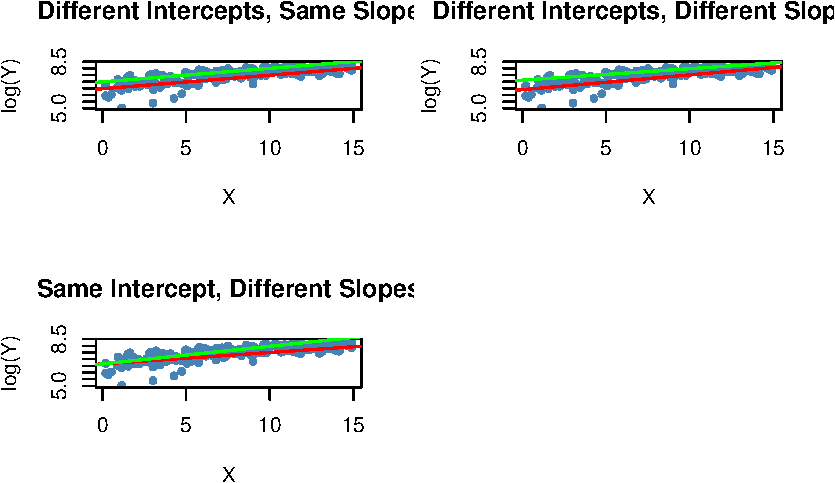
\includegraphics{URFITE_files/figure-latex/unnamed-chunk-41-1} \end{center}

We draw a sample of \(n=100\) observations and take the first
observation \(Y_1\) as an estimate for \(\mu_Y\)

\begin{Shaded}
\begin{Highlighting}[]
\CommentTok{# set seed for reproducibility}
\KeywordTok{set.seed}\NormalTok{(}\DecValTok{1}\NormalTok{)}

\CommentTok{# sample from the chi_12^2 distribution, keep only the first observation}
\KeywordTok{rchisq}\NormalTok{(}\DataTypeTok{n =} \DecValTok{100}\NormalTok{, }\DataTypeTok{df =} \DecValTok{12}\NormalTok{)[}\DecValTok{1}\NormalTok{]}
\end{Highlighting}
\end{Shaded}

\begin{verbatim}
## [1] 8.257893
\end{verbatim}

The estimate \(8.26\) is not too far away from \(\mu_Y = 12\) but it is
somewhat intuitive that we could do better: the estimator \(Y_1\)
discards a lot of information and its variance is the population
variance:

\[ \text{Var}(Y_1) = \text{Var}(Y) = 2 \cdot 12 = 24 \]

This brings us to the following question: What is a `good' estimator in
the first place? This question is tackled in Key Concepts 3.2 and 3.3

Key Concept 3.2

Bias, Consistency and Efficiency

Disirable characteristics of an estimator are unbiasedness, consitency
and Efficiency.

Unbiasedness:\\
If the mean of the sampling distribution of some estimator \(\hat\mu_Y\)
for the population mean \(\mu_Y\) equals \(\mu_Y\)
\[ E(\hat\mu_Y) = \mu_Y \] we say that the estimator is unbiased for
\(\mu_Y\). The \emph{bias} of \(\hat\mu_Y\) is \(0\):

\[ E(\hat\mu_Y) - \mu_Y = 0\]

Consistency:

We want the uncertainty of the estimator \(\mu_Y\) to decrease as the
number of observations in the sample grows. More precisely, we want the
proabability that the estimate \(\hat\mu_Y\) falls within a small
interval of the true value \(\mu_Y\) to get increasingly closer to \(1\)
as \(n\) grows. We write this as

\[ \hat\mu_Y \xrightarrow{p} \mu_Y. \]

Variance and efficiency:

We want the estimator to be efficient. Suppose we have two estimators,
\(\hat\mu_Y\) and \(\overset{\sim}{\mu}_Y\) and for some given sample
size \(n\) it holds that

\[ E(\hat\mu_Y) = E(\overset{\sim}{\mu}_Y) = \mu_Y \] but
\[\text{Var}(\hat\mu_Y) < \text{Var}(\overset{\sim}{\mu}_Y).\]

We then would prefer to use \(\hat\mu_Y\) as it has a lower variance
than \(\overset{\sim}{\mu}_Y\), meaning that \(\hat\mu_Y\) is more
\emph{efficient} in using the information provided by the observations
in the sample.

Key Concept 3.3

Efficiency of \(\overline{Y}\): The BLUE property

Let \(\hat\mu_Y\) be a linear and unbiased estimator of \(\mu_Y\) in the
fashion of

\[ \hat\mu_Y = \frac{1}{n} \sum_{i=1}^n a_i Y_i\]

with nonrandom constants \(a_i\). We see that \(\hat\mu_Y\) is a
weighted average of the \(Y_i\) and the \(a_i\) are weights. For these
type of estimators, \(\overline{Y}\) with \(a_i = 1\) for all
\(i = 1, \dots, n\) is the most efficient estimator. We say that
\(\overline{Y}\) is the BestLinear Unbiased Estimator (BLUE).

\section{Properties of the Sample
Mean}\label{properties-of-the-sample-mean}

To examine properties of the sample mean as an estimator for the
corresponding population mean, consider the following R example.

We generate a population \texttt{pop} which consists observations
\(Y_i \ , \ i=1,\dots,10000\) that stem from a normal distribution with
mean \(\mu = 10\) and variance \(\sigma^2 = 1\). To investigate how the
estimator \(\hat{\mu} = \bar{Y}\) behaves we can draw random samples
from this population and calculate \(\bar{Y}\) for each of them. This is
easily done by making use of the function \texttt{replicate()}. Its
argument \texttt{expr} is evaluated \texttt{n} times. In this case we
draw samples of sizes \(n=5\) and \(n=25\), compute the sample means and
repeat this exactly \(n=25000\) times.

For comparison purposes we store results for the estimator \(Y_1\), the
first observation in a sample for a sample of size \(5\) separately.

\begin{Shaded}
\begin{Highlighting}[]
\CommentTok{# generate a fictive population}
\NormalTok{pop <-}\StringTok{ }\KeywordTok{rnorm}\NormalTok{(}\DecValTok{10000}\NormalTok{, }\DecValTok{10}\NormalTok{, }\DecValTok{1}\NormalTok{)}

\CommentTok{# sample form pop and estimate the mean}
\NormalTok{est1 <-}\StringTok{ }\KeywordTok{replicate}\NormalTok{(}\DataTypeTok{expr =} \KeywordTok{mean}\NormalTok{(}\KeywordTok{sample}\NormalTok{(}\DataTypeTok{x =}\NormalTok{ pop, }\DataTypeTok{size =} \DecValTok{5}\NormalTok{)), }\DataTypeTok{n =} \DecValTok{25000}\NormalTok{)}

\NormalTok{est2 <-}\StringTok{ }\KeywordTok{replicate}\NormalTok{(}\DataTypeTok{expr =} \KeywordTok{mean}\NormalTok{(}\KeywordTok{sample}\NormalTok{(}\DataTypeTok{x =}\NormalTok{ pop, }\DataTypeTok{size =} \DecValTok{25}\NormalTok{)), }\DataTypeTok{n =} \DecValTok{25000}\NormalTok{)}

\NormalTok{fo <-}\StringTok{ }\KeywordTok{replicate}\NormalTok{(}\DataTypeTok{expr =} \KeywordTok{sample}\NormalTok{(}\DataTypeTok{x =}\NormalTok{ pop, }\DataTypeTok{size =} \DecValTok{5}\NormalTok{)[}\DecValTok{1}\NormalTok{], }\DataTypeTok{n =} \DecValTok{25000}\NormalTok{)}
\end{Highlighting}
\end{Shaded}

Check that \texttt{est1} and \texttt{est2} are vectors of length
\(25000\):

\begin{Shaded}
\begin{Highlighting}[]
\CommentTok{# check if object type is vector}
\KeywordTok{is.vector}\NormalTok{(est1)}
\end{Highlighting}
\end{Shaded}

\begin{verbatim}
## [1] TRUE
\end{verbatim}

\begin{Shaded}
\begin{Highlighting}[]
\KeywordTok{is.vector}\NormalTok{(est2)}
\end{Highlighting}
\end{Shaded}

\begin{verbatim}
## [1] TRUE
\end{verbatim}

\begin{Shaded}
\begin{Highlighting}[]
\CommentTok{# check lengths}
\KeywordTok{length}\NormalTok{(est1)}
\end{Highlighting}
\end{Shaded}

\begin{verbatim}
## [1] 25000
\end{verbatim}

\begin{Shaded}
\begin{Highlighting}[]
\KeywordTok{length}\NormalTok{(est2)}
\end{Highlighting}
\end{Shaded}

\begin{verbatim}
## [1] 25000
\end{verbatim}

The code chunk below produces a plot of the sampling distributions of
the estimators \(\bar{Y}\) and \(Y_1\) on the basis of the \(25000\)
samples in each case. We also plot a curve depicting the density
function of the \(N(10,1)\) distribution.

\begin{Shaded}
\begin{Highlighting}[]
\CommentTok{# plot density estimate Y_1}
\KeywordTok{plot}\NormalTok{(}\KeywordTok{density}\NormalTok{(fo), }
      \DataTypeTok{col =} \StringTok{'green'}\NormalTok{, }
      \DataTypeTok{lwd =} \DecValTok{2}\NormalTok{,}
      \DataTypeTok{ylim =} \KeywordTok{c}\NormalTok{(}\DecValTok{0}\NormalTok{,}\DecValTok{2}\NormalTok{),}
      \DataTypeTok{xlab =} \StringTok{'estimates'}\NormalTok{,}
      \DataTypeTok{main =} \StringTok{'Sampling Distributions of Unbiased Estimators'}
\NormalTok{      )}

\CommentTok{# add density estimate for the distribution of the sample mean with n=5 to the plot}
\KeywordTok{lines}\NormalTok{(}\KeywordTok{density}\NormalTok{(est1), }
     \DataTypeTok{col =} \StringTok{'steelblue'}\NormalTok{, }
     \DataTypeTok{lwd =} \DecValTok{2}\NormalTok{, }
     \DataTypeTok{bty =} \StringTok{'l'}
\NormalTok{     )}

\CommentTok{# add density estimate for the distribution of the sample mean with n=25 to the plot}
\KeywordTok{lines}\NormalTok{(}\KeywordTok{density}\NormalTok{(est2), }
      \DataTypeTok{col =} \StringTok{'red2'}\NormalTok{, }
      \DataTypeTok{lwd =} \DecValTok{2}
\NormalTok{      )}

\CommentTok{# add a vertical line marking the true parameter}
\KeywordTok{abline}\NormalTok{(}\DataTypeTok{v =} \DecValTok{10}\NormalTok{, }\DataTypeTok{lty =} \DecValTok{2}\NormalTok{)}

\CommentTok{# add N(10,1) density to the plot}
\KeywordTok{curve}\NormalTok{(}\KeywordTok{dnorm}\NormalTok{(x, }\DataTypeTok{mean=}\DecValTok{10}\NormalTok{), }
     \DataTypeTok{lwd =} \DecValTok{2}\NormalTok{,}
     \DataTypeTok{lty =} \DecValTok{2}\NormalTok{,}
     \DataTypeTok{add =}\NormalTok{ T}
\NormalTok{     )}

\CommentTok{# add a legend}
\KeywordTok{legend}\NormalTok{(}\StringTok{"topleft"}\NormalTok{,}
       \DataTypeTok{legend =} \KeywordTok{c}\NormalTok{(}\StringTok{"N(10,1)"}\NormalTok{,}
                  \KeywordTok{expression}\NormalTok{(Y[}\DecValTok{1}\NormalTok{]),}
                  \KeywordTok{expression}\NormalTok{(}\KeywordTok{bar}\NormalTok{(Y) }\OperatorTok{~}\StringTok{ }\NormalTok{n}\OperatorTok{==}\DecValTok{5}\NormalTok{),}
                  \KeywordTok{expression}\NormalTok{(}\KeywordTok{bar}\NormalTok{(Y) }\OperatorTok{~}\StringTok{ }\NormalTok{n}\OperatorTok{==}\DecValTok{25}\NormalTok{)}
\NormalTok{                  ), }
       \DataTypeTok{lty =} \KeywordTok{c}\NormalTok{(}\DecValTok{2}\NormalTok{, }\DecValTok{1}\NormalTok{, }\DecValTok{1}\NormalTok{, }\DecValTok{1}\NormalTok{), }
       \DataTypeTok{col =} \KeywordTok{c}\NormalTok{(}\StringTok{'black'}\NormalTok{,}\StringTok{'green'}\NormalTok{, }\StringTok{'steelblue'}\NormalTok{, }\StringTok{'red2'}\NormalTok{),}
       \DataTypeTok{lwd =} \DecValTok{2}
\NormalTok{       )}
\end{Highlighting}
\end{Shaded}

\begin{center}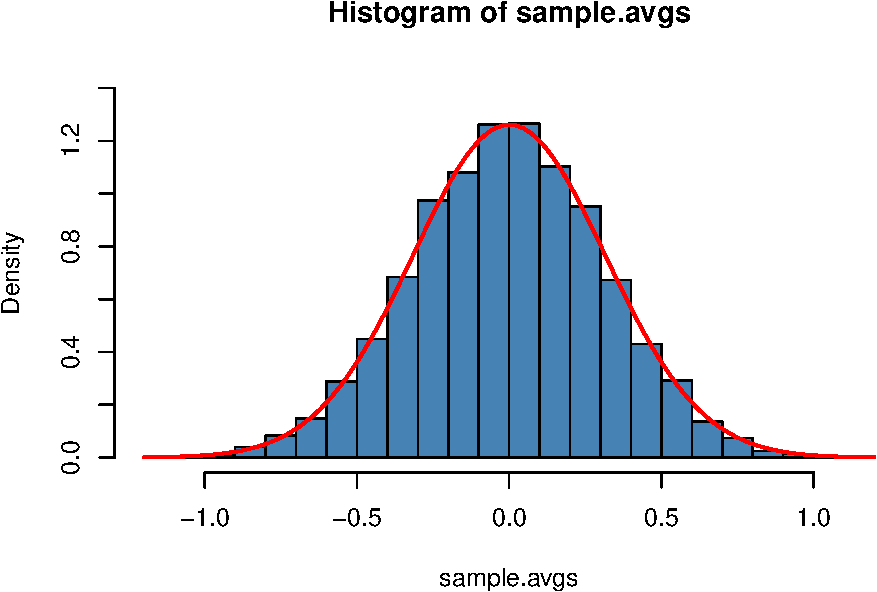
\includegraphics{URFITE_files/figure-latex/unnamed-chunk-45-1} \end{center}

At first, notice how \emph{all} sampling distributions (represented by
the solid lines) are centered around \(\mu = 10\). This is evidence for
the \emph{unbiasedness} of \(Y_1\) and \(\overline{Y}\). Of course, the
theoretical density the \(N(10,1)\) distribution is centered at \(10\),
too.

Next, have a look add the spread of the sampling distributions. Several
things are remarkable:

\begin{itemize}
\item
  First, the sampling distribution of \(Y_1\) (green curve) tracks the
  density of the \(N(10,1)\) distribution (black dashed line) pretty
  closely In fact, the sampling distribution of \(Y_1\) \emph{is} the
  \(N(10,1)\) distribution. This is less surprising if You keep in mind
  that \(Y_1\) estimator does nothing but reporting an observation that
  is randomly selected from a population with \(N(10,1)\) distribution.
  Hence, \(Y_1 \sim N(10,1)\). Note that this result is invariant to the
  sample size \(n\): the sampling distribution of \(Y_1\) is always the
  population distribution, no how large the sample is.
\item
  Second, both sampling distributions of \(\overline{Y}\) show less
  dispersion than the sampling distribution of \(Y_1\). This means that
  \(\overline{Y}\) has a lower variance than \(Y_1\). In view of Key
  Concepts 3.2 and 3.3, we find that \(\overline{Y}\) is a more
  efficient estimator than \(Y_1\). In fact, one can show that this
  holds for all \(n>1\).
\item
  Third, \(\overline{Y}\) shows a behaviour that is termed consistency
  (see Key Concept 3.2). Notice that the blue and the red density curves
  are much more concentrated around \(\mu=10\) then the green one. As
  the number of observations is increased from \(1\) to \(5\), the
  sampling distribution tightens around the true parameter. This effect
  is more dominant as the sample size is increased to \(25\). This
  implies that the probability of obtaining estimates that are close to
  the true value increases with \(n\).
\end{itemize}

\BeginKnitrBlock{rmdknit}
A more precise way to express consitency of an estimator \(\hat\mu\) for
a parameter \(\mu\) is

\[ P(|\hat{\mu} - \mu|<\epsilon) \xrightarrow[n \rightarrow \infty]{p} 1 \quad \text{for any}\quad\epsilon>0.\]

This expression says that the probability of observing a deviation from
the true value \(\mu\) that is smaller than some arbitrary
\(\epsilon > 0\) converges to \(1\) as \(n\) grows. Note that
consistency does not require unbiasedness:
\EndKnitrBlock{rmdknit}

We encourage You to go ahead and modify the code. Try out different
values for the sample size and see how the sampling distribution of
\(\overline{Y}\) changes!

\subsubsection*{\texorpdfstring{\(\overline{Y}\) is the least squares
estimator of
\(\mu_Y\)}{\textbackslash{}overline\{Y\} is the least squares estimator of \textbackslash{}mu\_Y}}\label{overliney-is-the-least-squares-estimator-of-mu_y}
\addcontentsline{toc}{subsubsection}{\(\overline{Y}\) is the least
squares estimator of \(\mu_Y\)}

Assume You have some observations \(Y_1,\dots,Y_n\) on
\(Y \sim N(10,1)\) (which is unknown) and would like to find an
estimator \(m\) that predicts the observations as good as possible where
good means to choose \(m\) such that the total deviation between the
predicted value and the observed values is small. Mathematically this
means we want to find an \(m\) that minimizes

\begin{equation}
  \sum_{i=1}^n (Y_i - m)^2. \label{eq:sqm}
\end{equation}

Think of \(Y_i - m\) as the comitted mistake when predicting \(Y_i\) by
\(m\). We could just as well minimize the sum of absolute deviations
from \(m\) but minimizing the sum of squared deviations is
mathematically more convenient and leads, roughly speaking, to the same
result. That is why the estimator we are looking for is called the
\emph{least squares estimator}. As It turns out \(m = \overline{Y}\),
the estimator of \(\mu_Y=10\) is this wanted estimator.

We can show this by generating a random sample of fair size and plotting
\eqref{eq:sqm} as a function of \(m\).

\begin{Shaded}
\begin{Highlighting}[]
\CommentTok{# define the function and vectorize it}
\NormalTok{sqm <-}\StringTok{ }\ControlFlowTok{function}\NormalTok{(m) \{}
 \KeywordTok{sum}\NormalTok{((y}\OperatorTok{-}\NormalTok{m)}\OperatorTok{^}\DecValTok{2}\NormalTok{)}
\NormalTok{\}}
\NormalTok{sqm <-}\StringTok{ }\KeywordTok{Vectorize}\NormalTok{(sqm)}

\CommentTok{# draw random sample and compute the mean}
\NormalTok{y <-}\StringTok{ }\KeywordTok{rnorm}\NormalTok{(}\DecValTok{100}\NormalTok{, }\DecValTok{10}\NormalTok{, }\DecValTok{1}\NormalTok{)}
\KeywordTok{mean}\NormalTok{(y)}
\end{Highlighting}
\end{Shaded}

\begin{verbatim}
## [1] 10.00543
\end{verbatim}

\begin{Shaded}
\begin{Highlighting}[]
\CommentTok{# plot the objective function}
\KeywordTok{curve}\NormalTok{(}\KeywordTok{sqm}\NormalTok{(x), }
      \DataTypeTok{from =} \OperatorTok{-}\DecValTok{50}\NormalTok{, }
      \DataTypeTok{to =} \DecValTok{70}\NormalTok{,}
      \DataTypeTok{xlab =} \StringTok{"m"}\NormalTok{,}
      \DataTypeTok{ylab =}\StringTok{"sqm(m)"}
\NormalTok{      )}

\CommentTok{# add vertical line at mean(y)}
\KeywordTok{abline}\NormalTok{(}\DataTypeTok{v =} \KeywordTok{mean}\NormalTok{(y), }
       \DataTypeTok{lty =} \DecValTok{2}\NormalTok{, }
       \DataTypeTok{col =} \StringTok{"darkred"}
\NormalTok{       )}
\end{Highlighting}
\end{Shaded}

\begin{center}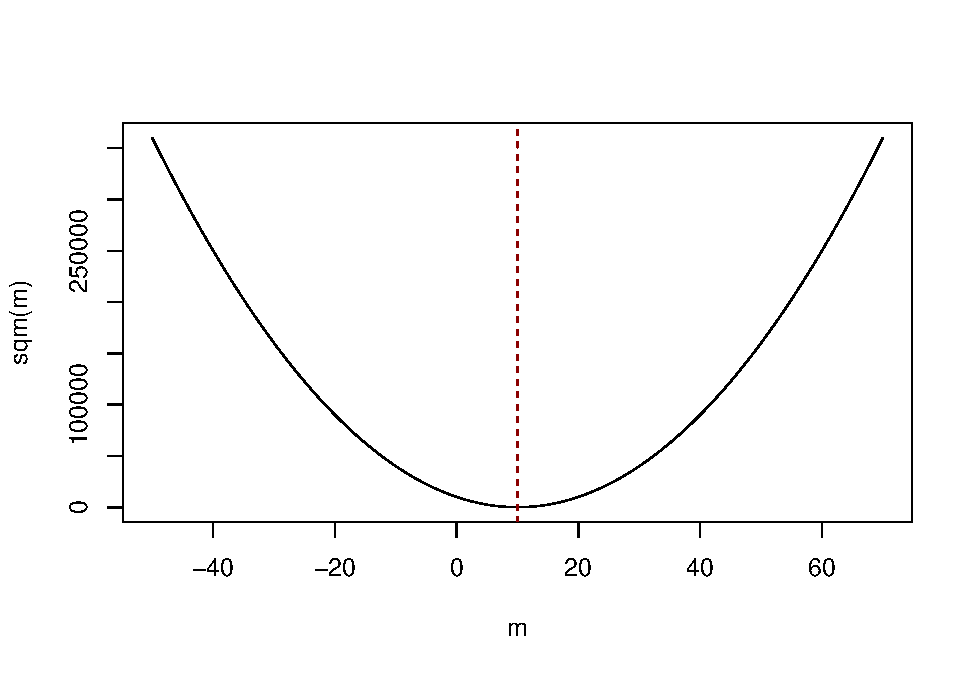
\includegraphics{URFITE_files/figure-latex/unnamed-chunk-46-1} \end{center}

Notice that \eqref{eq:sqm} is a quadratic function so there is only one
minimum. The plot shows that this minimum lies exactly at the sample
mean of the sample data.

\BeginKnitrBlock{rmdknit}
Some R functions can only interact with functions that take a vector as
input evaluate the function body on every values of the vector, for
example curve(). We call such functions vectorized functions and it is
often a good idea to write vectorized functions although this is
cumbersome in some cases. Having a vectorized function in R is never a
drawback since these functions work on both single values and vectors.

Let us look at the function sqm() which is nonvectorized

 sqm \textless{}- function(m) \{\\
\hspace*{0.333em}\hspace*{0.333em}\hspace*{0.333em}\hspace*{0.333em}
sum((y-m)\^{}2) \#body of the function\\
\}

Providing e.g. c(1,2,3) as the argument m would cause an error since
then the operation y-m is invalid: the vecors y and m are of
incompatible dimensions. This is why we cannot use sqm() in conjunction
with curve().

Here comes Vectorize() into play. It generates a vectorized version of a
non-vectorized function.
\EndKnitrBlock{rmdknit}

\subsubsection*{Why Random Sampling is
important}\label{why-random-sampling-is-important}
\addcontentsline{toc}{subsubsection}{Why Random Sampling is important}

So far, we assumed (somtimes implicitly) that observed data
\(Y_1, \dots, Y_n\) are the result of a sampling process that satisfies
the assumption of i.i.d. random sampling. It is very important that this
assumption is fulfilled when estimating a population mean using
\(\overline{Y}\). If this is not the case, estimates are biased.

Let us fall back to \texttt{pop}, the fictive population of \(10000\)
observations and compute the population mean \(\mu_{\texttt{pop}}\):

\begin{Shaded}
\begin{Highlighting}[]
\CommentTok{# compute the population mean of pop}
\KeywordTok{mean}\NormalTok{(pop)}
\end{Highlighting}
\end{Shaded}

\begin{verbatim}
## [1] 9.992604
\end{verbatim}

Next we sample \(10\) observations from \texttt{pop} with
\texttt{sample()} and estimate \(\mu_{\texttt{pop}}\) using
\(\overline{Y}\) repeatedly. However this time we use a sampling scheme
that deviates from simple random sampling: instead of ensuring that each
member of the population has the same chance to end up in a sample, we
assign a higher probability of beeing sampled to the \(2500\) smallest
observations of the population by setting the argument \texttt{prop} to
a suitable vector of probability weights:

\begin{Shaded}
\begin{Highlighting}[]
\CommentTok{# simulate outcome for the sample mean when the i.i.d. assumption fails}
\NormalTok{est3 <-}\StringTok{  }\KeywordTok{replicate}\NormalTok{(}\DataTypeTok{n =} \DecValTok{25000}\NormalTok{, }
                    \DataTypeTok{expr =} \KeywordTok{mean}\NormalTok{(}\KeywordTok{sample}\NormalTok{(}\DataTypeTok{x =} \KeywordTok{sort}\NormalTok{(pop), }
                                  \DataTypeTok{size =} \DecValTok{10}\NormalTok{, }
                                  \DataTypeTok{prob =} \KeywordTok{c}\NormalTok{(}\KeywordTok{rep}\NormalTok{(}\DecValTok{4}\NormalTok{,}\DecValTok{2500}\NormalTok{),}\KeywordTok{rep}\NormalTok{(}\DecValTok{1}\NormalTok{,}\DecValTok{7500}\NormalTok{))}
\NormalTok{                                      )}
\NormalTok{                                )}
\NormalTok{                   )}

\CommentTok{# compute the sample mean of the outcomes}
\KeywordTok{mean}\NormalTok{(est3)}
\end{Highlighting}
\end{Shaded}

\begin{verbatim}
## [1] 9.443454
\end{verbatim}

Next we plot the sampling distribution of \(\overline{Y}\) for this
non-i.i.d. case an compare it to the sampling distribution when the
i.i.d. assumption holds.

\begin{Shaded}
\begin{Highlighting}[]
\CommentTok{# sampling distribution of sample mean, i.i.d. holds, n=25}
\KeywordTok{plot}\NormalTok{(}\KeywordTok{density}\NormalTok{(est2), }
      \DataTypeTok{col =} \StringTok{'red2'}\NormalTok{,}
      \DataTypeTok{lwd =} \DecValTok{2}\NormalTok{,}
      \DataTypeTok{xlim =} \KeywordTok{c}\NormalTok{(}\DecValTok{8}\NormalTok{,}\DecValTok{11}\NormalTok{),}
      \DataTypeTok{xlab =} \StringTok{'estimates'}\NormalTok{,}
      \DataTypeTok{main =} \StringTok{'When the i.i.d. Assumption Fails'}
\NormalTok{     )}

\CommentTok{# sampling distribution of sample mean, i.i.d. fails, n=25}
\KeywordTok{lines}\NormalTok{(}\KeywordTok{density}\NormalTok{(est3),}
      \DataTypeTok{col =} \StringTok{'steelblue'}\NormalTok{,}
      \DataTypeTok{lwd =} \DecValTok{2}
\NormalTok{      )}

\CommentTok{# add a legend}
\KeywordTok{legend}\NormalTok{(}\StringTok{"topleft"}\NormalTok{,}
       \DataTypeTok{legend =} \KeywordTok{c}\NormalTok{(}\KeywordTok{expression}\NormalTok{(}\KeywordTok{bar}\NormalTok{(Y) }\OperatorTok{~}\StringTok{ ","} \OperatorTok{~}\StringTok{ }\NormalTok{n}\OperatorTok{==}\DecValTok{25} \OperatorTok{~}\StringTok{ ", i.i.d. fails"}\NormalTok{),}
                  \KeywordTok{expression}\NormalTok{(}\KeywordTok{bar}\NormalTok{(Y) }\OperatorTok{~}\StringTok{ ","} \OperatorTok{~}\StringTok{ }\NormalTok{n}\OperatorTok{==}\DecValTok{25} \OperatorTok{~}\StringTok{ ", i.i.d. holds"}\NormalTok{)}
\NormalTok{                  ), }
       \DataTypeTok{lty =} \KeywordTok{c}\NormalTok{(}\DecValTok{1}\NormalTok{, }\DecValTok{1}\NormalTok{), }
       \DataTypeTok{col =} \KeywordTok{c}\NormalTok{(}\StringTok{'red2'}\NormalTok{, }\StringTok{'steelblue'}\NormalTok{),}
       \DataTypeTok{lwd =} \DecValTok{2}
\NormalTok{       )}
\end{Highlighting}
\end{Shaded}

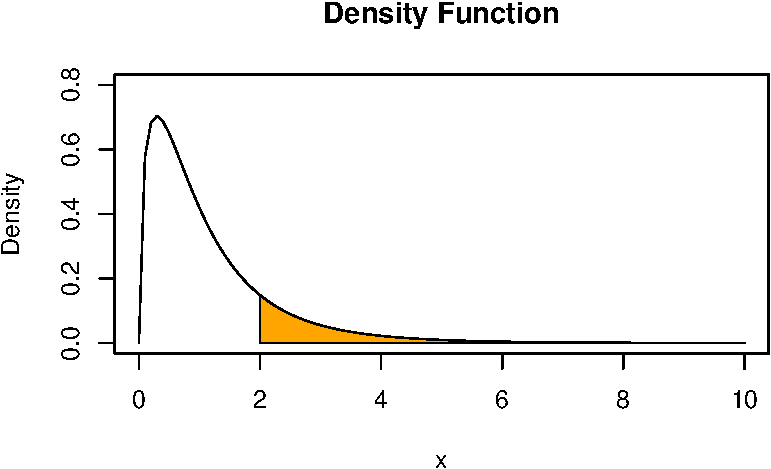
\includegraphics{URFITE_files/figure-latex/unnamed-chunk-49-1.pdf}

We find that in this case failure of the i.i.d. assumption implies that,
on average, we underestimate \(\mu_Y\) using \(\overline{Y}\): the
corresponding distribution of \(\overline{Y}\) is shifted to the left.
In other words, \(\overline{Y}\) is a \emph{biased} estimator for
\(\mu_Y\) if the i.i.d. assumption does not hold.

\section{Hypothesis Tests Concerning the Population
Mean}\label{hypothesis-tests-concerning-the-population-mean}

In this section we briefly review concepts in hypothesis testing and
discuss how to conduct hypothesis tests in R. We focus on drawing
inference about an unkown population mean.

\subsubsection*{About Hypotheses and Hypothesis
Testing}\label{about-hypotheses-and-hypothesis-testing}
\addcontentsline{toc}{subsubsection}{About Hypotheses and Hypothesis
Testing}

In a significance test we want to exploit the information contained in a
random sample as evidence in favour or against a hypothesis.
Essentially, hypotheses are simple question that can be answered by
`yes' or `no'. When conducting a hypothesis test we always deal with two
different hypotheses:

\begin{itemize}
\item
  The null hypothesis, denoted \(H_0\) is the hypothesis we are
  interested in testing
\item
  The alternative hypothesis, denoted \(H_1\), is the hypothesis that
  holds if the null hypothesis is false
\end{itemize}

The null hypothesis that the population mean of \(Y\) equals the value
\(\mu_{Y,0}\) is written down as

\[ H_0: E(Y) = \mu_{Y,0}. \]

The alternative hypothesis states what holds if the null hypothesis is
false. Often the alternative hypothesis chosen is the most general one,

\[ H_1: E(Y) \neq \mu_{Y,0}, \]

meaning that \(E(Y)\) may be anything else but the value as the null
hypothesis. This is called a two-sided alternative.

For brevity, we will only consider the case of a two-sided alternative
in the subsequent sections of this chapter.

\subsection*{\texorpdfstring{\(p\)-Value}{p-Value}}\label{p-value}
\addcontentsline{toc}{subsection}{\(p\)-Value}

Assume that the null hypothesis is \emph{true}. The \(p\)-value is the
probability of drawing data and observing a corresponding test
statistics that is at least as adverse to what is stated under the null
hypothesis as the test statistic actually computed using the sample
data.

In context of population mean and sample mean, this definition can be
stated mathematically in the following way:

\begin{equation}
p \text{-value} = P_{H_0}\left[ \lvert \overline{Y} - \mu_{Y,0} \rvert > \lvert \overline{Y}^{act} - \mu_{Y,0} \rvert \right] \label{eq:pvalue}
\end{equation}

In \eqref{eq:pvalue}, \(\overline{Y}^{act}\) is the acutally computed mean
of the random sample. Visualized, the \(p\)-value is the area in the
part of tails of the distribution of \(\overline{Y}\) that lies beyond

\[ \mu_{Y,0} \pm \lvert \overline{Y}^{act} - \mu_{Y,0} \rvert. \]

Consequently, in order to compute the \(p\)-value as in \eqref{eq:pvalue},
knowledge about the sampling distribution of \(\overline{Y}\) when the
null hypothesis is true is required. However in most cases the sampling
distribution of \(\overline{Y}\) is unkown. Furtunately, due to the
large-sample normal approximation (see chapter 3) we know that under the
null hypothesis

\[ \overline{Y} \sim N(\mu_{Y,0}, \, \sigma^2_{\overline{Y}}) \ \ , \ \ \sigma^2_{\overline{Y}} = \frac{\sigma_Y^2}{n} \]

and thus

\[ \frac{\overline{Y} - \mu_{Y,0}}{\sigma_Y/\sqrt{n}} \sim N(0,1). \]

So in large samples, the \(p\)-value can be computed \emph{without}
knowledge about the sampling distribution of \(\overline{Y}\).

\subsection*{\texorpdfstring{Calculating the \(p\)-Value When
\(\sigma_Y\) Is
Known}{Calculating the p-Value When \textbackslash{}sigma\_Y Is Known}}\label{calculating-the-p-value-when-sigma_y-is-known}
\addcontentsline{toc}{subsection}{Calculating the \(p\)-Value When
\(\sigma_Y\) Is Known}

For now, let us assume that \(\sigma_{\overline{Y}}\) is known. Then we
can rewrite \eqref{eq:pvalue} as

\begin{align}
p \text{-value} =& \, P_{H_0}\left[ \left\lvert \frac{\overline{Y} - \mu_{Y,0}}{\sigma_{\overline{Y}}} \right\rvert > \left\lvert \frac{\overline{Y}^{act} - \mu_{Y,0}}{\sigma_{\overline{Y}}} \right\rvert \right] \\
=& \, 2 \cdot \Phi \left[ - \left\lvert \frac{\overline{Y}^{act} - \mu_{Y,0}}{\sigma_{\overline{Y}}}  \right\rvert\right].  \label{eq:pvaluenorm1}
\end{align}

so the \(p\)-value can be seen as the area in the tails of the
\(N(0,1)\) distribution that lies beyond

\begin{equation}
\pm \left\lvert \frac{\overline{Y}^{act} - \mu_{Y,0}}{\sigma_{\overline{Y}}} \right\rvert \label{eq:pvaluenorm2}
\end{equation}

Whew, that was a lot of theory. Now we use R to visualize what is stated
in \eqref{eq:pvaluenorm1} and \eqref{eq:pvaluenorm2}. The next code chunck
replicates figure 3.1 of the book.

\begin{Shaded}
\begin{Highlighting}[]
\CommentTok{# plot the standard normal density on the domain [-4,4]}
\KeywordTok{curve}\NormalTok{(}\KeywordTok{dnorm}\NormalTok{(x),}
      \DataTypeTok{xlim =} \KeywordTok{c}\NormalTok{(}\OperatorTok{-}\DecValTok{4}\NormalTok{,}\DecValTok{4}\NormalTok{),}
      \DataTypeTok{main =} \StringTok{'Calculating a p-value'}\NormalTok{,}
      \DataTypeTok{yaxs =} \StringTok{'i'}\NormalTok{,}
      \DataTypeTok{xlab =} \StringTok{'z'}\NormalTok{,}
      \DataTypeTok{ylab =} \StringTok{''}\NormalTok{,}
      \DataTypeTok{lwd =} \DecValTok{2}\NormalTok{,}
      \DataTypeTok{axes =} \StringTok{'F'}
\NormalTok{      )}

\CommentTok{# add x-axis}
\KeywordTok{axis}\NormalTok{(}\DecValTok{1}\NormalTok{, }
     \DataTypeTok{at =} \KeywordTok{c}\NormalTok{(}\OperatorTok{-}\FloatTok{1.5}\NormalTok{,}\DecValTok{0}\NormalTok{,}\FloatTok{1.5}\NormalTok{), }
     \DataTypeTok{padj =} \FloatTok{0.75}\NormalTok{,}
     \DataTypeTok{labels =} \KeywordTok{c}\NormalTok{(}\KeywordTok{expression}\NormalTok{(}\OperatorTok{-}\KeywordTok{frac}\NormalTok{(}\KeywordTok{bar}\NormalTok{(Y)}\OperatorTok{^}\StringTok{"act"}\OperatorTok{~-}\ErrorTok{~}\KeywordTok{bar}\NormalTok{(mu)[Y,}\DecValTok{0}\NormalTok{],sigma[}\KeywordTok{bar}\NormalTok{(Y)])),}
                \DecValTok{0}\NormalTok{,}
                \KeywordTok{expression}\NormalTok{(}\KeywordTok{frac}\NormalTok{(}\KeywordTok{bar}\NormalTok{(Y)}\OperatorTok{^}\StringTok{"act"}\OperatorTok{~-}\ErrorTok{~}\KeywordTok{bar}\NormalTok{(mu)[Y,}\DecValTok{0}\NormalTok{],sigma[}\KeywordTok{bar}\NormalTok{(Y)])))}
\NormalTok{     )}

\CommentTok{# shade p-value/2 region in left tail}
\KeywordTok{polygon}\NormalTok{(}\DataTypeTok{x =} \KeywordTok{c}\NormalTok{(}\OperatorTok{-}\DecValTok{6}\NormalTok{, }\KeywordTok{seq}\NormalTok{(}\OperatorTok{-}\DecValTok{6}\NormalTok{,}\OperatorTok{-}\FloatTok{1.5}\NormalTok{,}\FloatTok{0.01}\NormalTok{),}\OperatorTok{-}\FloatTok{1.5}\NormalTok{),}
        \DataTypeTok{y =} \KeywordTok{c}\NormalTok{(}\DecValTok{0}\NormalTok{, }\KeywordTok{dnorm}\NormalTok{(}\KeywordTok{seq}\NormalTok{(}\OperatorTok{-}\DecValTok{6}\NormalTok{,}\OperatorTok{-}\FloatTok{1.5}\NormalTok{,}\FloatTok{0.01}\NormalTok{)),}\DecValTok{0}\NormalTok{), }
        \DataTypeTok{col =} \StringTok{'steelblue'}
\NormalTok{        )}

\NormalTok{## shade p-value/2 region in right tail}
\KeywordTok{polygon}\NormalTok{(}\DataTypeTok{x =} \KeywordTok{c}\NormalTok{(}\FloatTok{1.5}\NormalTok{, }\KeywordTok{seq}\NormalTok{(}\FloatTok{1.5}\NormalTok{, }\DecValTok{6}\NormalTok{, }\FloatTok{0.01}\NormalTok{), }\DecValTok{6}\NormalTok{),}
        \DataTypeTok{y =} \KeywordTok{c}\NormalTok{(}\DecValTok{0}\NormalTok{, }\KeywordTok{dnorm}\NormalTok{(}\KeywordTok{seq}\NormalTok{(}\FloatTok{1.5}\NormalTok{, }\DecValTok{6}\NormalTok{, }\FloatTok{0.01}\NormalTok{)), }\DecValTok{0}\NormalTok{), }
        \DataTypeTok{col =} \StringTok{'steelblue'}
\NormalTok{        )}
\end{Highlighting}
\end{Shaded}

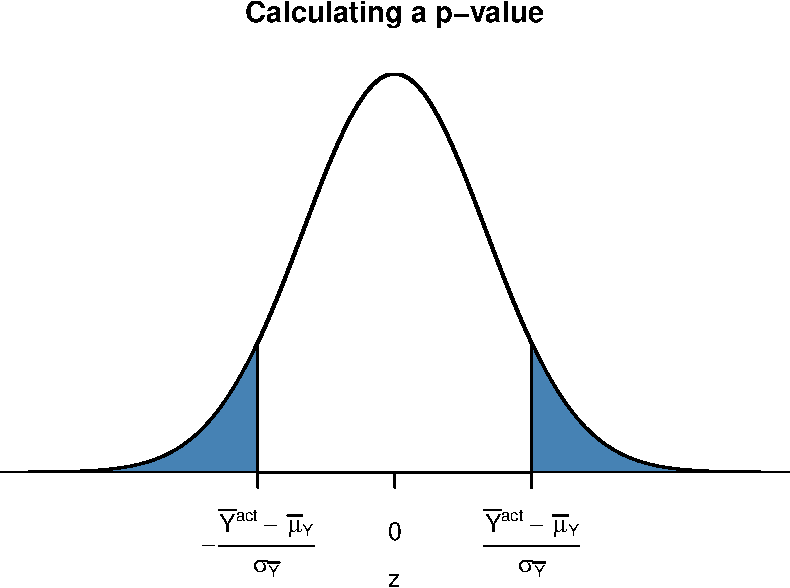
\includegraphics{URFITE_files/figure-latex/unnamed-chunk-50-1.pdf}

\subsection*{Sample Variance, Sample Standard Deviation and Standard
Error}\label{sample-variance-sample-standard-deviation-and-standard-error}
\addcontentsline{toc}{subsection}{Sample Variance, Sample Standard
Deviation and Standard Error}

If \(\sigma^2_Y\) is unknown, it must be estimated. This can be done
efficiently using the sample variance

\begin{equation}
s_y^2 = \frac{1}{n-1} \sum_{i=1}^n (Y_i - \overline{Y})^2.
\end{equation}

Furthermore

\begin{equation}
s_y = \sqrt{\frac{1}{n-1} \sum_{i=1}^n (Y_i - \overline{Y})^2}.
\end{equation}

is a suitable estimator for the standard deviation of \(Y\). In R,
\(s_y\) is implemented in the function \texttt{sd()}, see \texttt{?sd}.

Using R we can get a notion that \(s_y\) is a consistent estimator for
\(\sigma_Y\), that is

\[ s_Y \overset{p}{\longrightarrow} \sigma_Y. \]

The idea here is to generate a large number of samples \(Y_1,\dots,Y_n\)
where \(Y\sim N(10,10)\), estimate \(\sigma_Y\) using \(s_y\) and
investigate how the distribution of \(s_Y\) changes as \(n\) grows.

\begin{Shaded}
\begin{Highlighting}[]
\CommentTok{# vector of sample sizes}
\NormalTok{n <-}\StringTok{ }\KeywordTok{c}\NormalTok{(}\DecValTok{10000}\NormalTok{, }\DecValTok{5000}\NormalTok{, }\DecValTok{2000}\NormalTok{, }\DecValTok{1000}\NormalTok{, }\DecValTok{500}\NormalTok{)}

\CommentTok{# sample observations, estimate using sd() and plot estimated distributions}
\NormalTok{s2_y <-}\StringTok{ }\KeywordTok{replicate}\NormalTok{(}\DataTypeTok{n =} \DecValTok{10000}\NormalTok{, }\DataTypeTok{expr =} \KeywordTok{sd}\NormalTok{(}\KeywordTok{rnorm}\NormalTok{(n[}\DecValTok{1}\NormalTok{], }\DecValTok{10}\NormalTok{, }\DecValTok{10}\NormalTok{)))}
\KeywordTok{plot}\NormalTok{(}\KeywordTok{density}\NormalTok{(s2_y),}
     \DataTypeTok{main =} \KeywordTok{expression}\NormalTok{(}\StringTok{'Sampling Distributions of'} \OperatorTok{~}\StringTok{ }\NormalTok{s[y]),}
     \DataTypeTok{xlab =} \KeywordTok{expression}\NormalTok{(s[y]),}
     \DataTypeTok{lwd =} \DecValTok{2}
\NormalTok{     )}

\ControlFlowTok{for}\NormalTok{ (i }\ControlFlowTok{in} \DecValTok{2}\OperatorTok{:}\KeywordTok{length}\NormalTok{(n)) \{}
\NormalTok{  s2_y <-}\StringTok{ }\KeywordTok{replicate}\NormalTok{(}\DataTypeTok{n =} \DecValTok{10000}\NormalTok{, }\DataTypeTok{expr =} \KeywordTok{sd}\NormalTok{(}\KeywordTok{rnorm}\NormalTok{(n[i],}\DecValTok{10}\NormalTok{,}\DecValTok{10}\NormalTok{)))}
  \KeywordTok{lines}\NormalTok{(}\KeywordTok{density}\NormalTok{(s2_y), }
        \DataTypeTok{col=}\NormalTok{i, }
        \DataTypeTok{lwd=}\DecValTok{2}\NormalTok{)}
\NormalTok{\}}

\CommentTok{# add a legend}
\KeywordTok{legend}\NormalTok{(}\StringTok{"topleft"}\NormalTok{,}
       \DataTypeTok{legend =} \KeywordTok{c}\NormalTok{(}\KeywordTok{expression}\NormalTok{(n}\OperatorTok{==}\DecValTok{10000}\NormalTok{),}
                  \KeywordTok{expression}\NormalTok{(n}\OperatorTok{==}\DecValTok{5000}\NormalTok{),}
                  \KeywordTok{expression}\NormalTok{(n}\OperatorTok{==}\DecValTok{2000}\NormalTok{),}
                  \KeywordTok{expression}\NormalTok{(n}\OperatorTok{==}\DecValTok{1000}\NormalTok{),}
                  \KeywordTok{expression}\NormalTok{(n}\OperatorTok{==}\DecValTok{500}\NormalTok{)}
\NormalTok{       ), }
       \DataTypeTok{col =} \DecValTok{1}\OperatorTok{:}\DecValTok{5}\NormalTok{,}
       \DataTypeTok{lwd =} \DecValTok{2}
\NormalTok{)}
\end{Highlighting}
\end{Shaded}

\begin{center}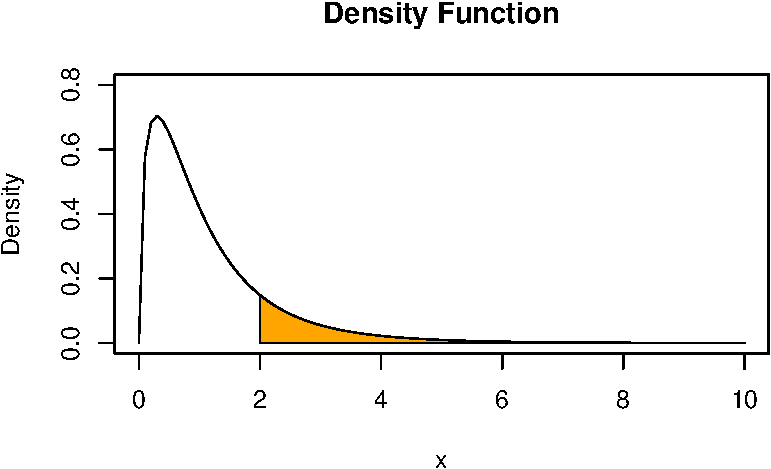
\includegraphics{URFITE_files/figure-latex/unnamed-chunk-51-1} \end{center}

The plot shows that the distribution of \(s_Y\) tightens around the true
value \(\sigma_Y = 10\) as \(n\) increases.

The function that estimates the standard deviation of an estimator is
called the \emph{standard error of the estimator}. Key Concept 3.4
summarizes the terminology in the context of the sample mean.

Key Concept 3.4

The Standard Error of \(\overline{Y}\)

Take an i.i.d. sample \(Y_1, \dots, Y_n\). The mean of \(Y\) can be
consistently estimated using \(\overline{Y}\), the sample mean of the
\(Y_i\). Since \(\overline{Y}\) is a random variable, it has a sampling
distribution with variance \(\frac{\sigma_Y^2}{n}\).

The standard error of \(\overline{Y}\), denoted \(SE(\overline{Y})\) is
an estimator of the standard deviation \(\overline{Y}\):

\[ SE(\overline{Y}) = \hat\sigma_{\overline{Y}} = \frac{s_Y}{\sqrt{n}} \]

The caret (\^{}) over \(\sigma\) indicates that
\(\hat\sigma_{\overline{Y}}\) is an estimator for
\(\sigma_{\overline{Y}}\).

As an example to underpin Key Concept 3.4, consider a sample of
\(n=100\) i.i.d. observations of the bernoulli distributed variable
\(Y\) with success probability \(p=0.1\) and thus \(E(Y)=p=0.1\) and
\(\text{Var}(Y)=p(1-p)\). \(E(Y)\) can be estimated by \(\overline{Y}\)
which then has variance

\[ \sigma^2_{\overline{Y}} = p(1-p)/n = 0.0009 \]

and standard deviation

\[ \sigma_{\overline{Y}} = \sqrt{p(1-p)/n} = 0.03. \]

In this case the standard error of \(\overline{Y}\) is given as

\[ SE(\overline{Y}) = \sqrt{\overline{Y}(1-\overline{Y})/n} \]

Let verify whether \(\overline{Y}\) and \(SE(\overline{Y})\) estimate
the respective true values on average.

\begin{Shaded}
\begin{Highlighting}[]
\CommentTok{# draw 10000 samples of size 100 and estimate the mean of Y and}
\CommentTok{# estimate the standard error of the sample mean}

\NormalTok{mean_estimates <-}\StringTok{ }\KeywordTok{numeric}\NormalTok{(}\DecValTok{10000}\NormalTok{)}
\NormalTok{se_estimates <-}\StringTok{ }\KeywordTok{numeric}\NormalTok{(}\DecValTok{10000}\NormalTok{)}

\ControlFlowTok{for}\NormalTok{ (i }\ControlFlowTok{in} \DecValTok{1}\OperatorTok{:}\DecValTok{10000}\NormalTok{) \{}
\NormalTok{  s <-}\StringTok{ }\KeywordTok{sample}\NormalTok{(}\DecValTok{0}\OperatorTok{:}\DecValTok{1}\NormalTok{, }
              \DataTypeTok{size =} \DecValTok{100}\NormalTok{,  }
              \DataTypeTok{prob =} \KeywordTok{c}\NormalTok{(}\FloatTok{0.9}\NormalTok{, }\FloatTok{0.1}\NormalTok{),}
              \DataTypeTok{replace =}\NormalTok{ T}
\NormalTok{              )}
\NormalTok{  mean_estimates[i] <-}\StringTok{ }\KeywordTok{mean}\NormalTok{(s)}
\NormalTok{  se_estimates[i] <-}\StringTok{ }\KeywordTok{sqrt}\NormalTok{(}\KeywordTok{mean}\NormalTok{(s)}\OperatorTok{*}\NormalTok{(}\DecValTok{1}\OperatorTok{-}\KeywordTok{mean}\NormalTok{(s))}\OperatorTok{/}\DecValTok{100}\NormalTok{)}
\NormalTok{\}}

\KeywordTok{mean}\NormalTok{(mean_estimates)}
\end{Highlighting}
\end{Shaded}

\begin{verbatim}
## [1] 0.099693
\end{verbatim}

\begin{Shaded}
\begin{Highlighting}[]
\KeywordTok{mean}\NormalTok{(se_estimates)}
\end{Highlighting}
\end{Shaded}

\begin{verbatim}
## [1] 0.02953467
\end{verbatim}

Both estimators seem to be unbiased for the true parameters.

\subsection*{\texorpdfstring{Calculating the \(p\)-value When
\(\sigma_Y\) is
Unknown}{Calculating the p-value When \textbackslash{}sigma\_Y is Unknown}}\label{calculating-the-p-value-when-sigma_y-is-unknown}
\addcontentsline{toc}{subsection}{Calculating the \(p\)-value When
\(\sigma_Y\) is Unknown}

When \(\sigma_Y\) is unkown, the \(p\)-value for a hypothesis test about
\(\mu_Y\) using \(\overline{Y}\) can be computed by replacing
\(\sigma_{\overline{Y}}\) in \eqref{eq:pvaluenorm1} by the standard error
\(SE(\overline{Y}) = \hat\sigma_Y\). Then,

\[ p\text{-value} = 2\cdot\Phi\left(-\left\lvert \frac{\overline{Y}^{act}-\mu_{Y,0}}{SE(\overline{Y})} \right\rvert \right). \]

This is easily done in R:

\begin{Shaded}
\begin{Highlighting}[]
\CommentTok{# sample and estimate, compute standard error and make a hypothesis}
\NormalTok{samplemean_act <-}\StringTok{ }\KeywordTok{mean}\NormalTok{(}
  \KeywordTok{sample}\NormalTok{(}\DecValTok{0}\OperatorTok{:}\DecValTok{1}\NormalTok{, }
         \DataTypeTok{prob =} \KeywordTok{c}\NormalTok{(}\FloatTok{0.9}\NormalTok{,}\FloatTok{0.1}\NormalTok{), }
         \DataTypeTok{replace =}\NormalTok{ T, }
         \DataTypeTok{size =} \DecValTok{100}
\NormalTok{         )}
\NormalTok{  )}

\NormalTok{SE_samplemean <-}\StringTok{ }\KeywordTok{sqrt}\NormalTok{(samplemean_act }\OperatorTok{*}\StringTok{ }\NormalTok{(}\DecValTok{1}\OperatorTok{-}\NormalTok{samplemean_act)}\OperatorTok{/}\DecValTok{100}\NormalTok{)}

\NormalTok{mean_h0 <-}\StringTok{ }\FloatTok{0.1} \CommentTok{#true null hypothesis}

\CommentTok{# compute the pvalue}
\NormalTok{pvalue <-}\StringTok{ }\DecValTok{2} \OperatorTok{*}\StringTok{ }\KeywordTok{pnorm}\NormalTok{(}\OperatorTok{-}\KeywordTok{abs}\NormalTok{(samplemean_act}\OperatorTok{-}\NormalTok{mean_h0)}\OperatorTok{/}\NormalTok{SE_samplemean)}
\NormalTok{pvalue}
\end{Highlighting}
\end{Shaded}

\begin{verbatim}
## [1] 0.5382527
\end{verbatim}

\subsection*{\texorpdfstring{The
\(t\)-statistic}{The t-statistic}}\label{the-t-statistic}
\addcontentsline{toc}{subsection}{The \(t\)-statistic}

In hypothesis testing, the standardized sample average

\begin{equation}
t = \frac{\overline{Y} - \mu_{Y,0}}{SE(\overline{Y})} \label{eq:tstat}
\end{equation}

is called \(t\)-statistic. This \(t\)-statistic has an important role
when testing hypothesis about \(\mu_Y\). It is a prominent example of a
test statistic.

Implicitly, we already have computed a \(t\)-statistic for
\(\overline{Y}\) in the previous code chunk.

\begin{Shaded}
\begin{Highlighting}[]
\CommentTok{# compute a t-statistic for the sample mean}
\NormalTok{tstatistic <-}\StringTok{ }\NormalTok{(samplemean_act }\OperatorTok{-}\StringTok{ }\NormalTok{mean_h0) }\OperatorTok{/}\StringTok{ }\NormalTok{SE_samplemean}
\NormalTok{tstatistic}
\end{Highlighting}
\end{Shaded}

\begin{verbatim}
## [1] 0.6154575
\end{verbatim}

Using R we can show that if \(\mu_{Y,0}\) equals the true value, that is
the null hypothesis is true, \eqref{eq:tstat} is approximately distributed
\(N(0,1)\) when \(n\) is large.

\begin{Shaded}
\begin{Highlighting}[]
\CommentTok{# initialize empty vector for t-statistics}
\NormalTok{tstatistics <-}\StringTok{ }\KeywordTok{numeric}\NormalTok{(}\DecValTok{10000}\NormalTok{)}

\CommentTok{# set sample size}
\NormalTok{n <-}\StringTok{ }\DecValTok{300}

\CommentTok{# simulate 10000 t-statistics}
\ControlFlowTok{for}\NormalTok{ (i }\ControlFlowTok{in} \DecValTok{1}\OperatorTok{:}\DecValTok{10000}\NormalTok{) \{}
\NormalTok{  s <-}\StringTok{ }\KeywordTok{sample}\NormalTok{(}\DecValTok{0}\OperatorTok{:}\DecValTok{1}\NormalTok{, }
              \DataTypeTok{size =}\NormalTok{ n,  }
              \DataTypeTok{prob =} \KeywordTok{c}\NormalTok{(}\FloatTok{0.9}\NormalTok{, }\FloatTok{0.1}\NormalTok{),}
              \DataTypeTok{replace =}\NormalTok{ T}
\NormalTok{              )}
\NormalTok{  tstatistics[i] <-}\StringTok{ }\NormalTok{(}\KeywordTok{mean}\NormalTok{(s)}\OperatorTok{-}\FloatTok{0.1}\NormalTok{)}\OperatorTok{/}\NormalTok{(}\KeywordTok{sqrt}\NormalTok{(}\KeywordTok{mean}\NormalTok{(s)}\OperatorTok{*}\NormalTok{(}\DecValTok{1}\OperatorTok{-}\KeywordTok{mean}\NormalTok{(s))}\OperatorTok{/}\NormalTok{n))}
\NormalTok{\}}

\CommentTok{# plot density and compare to N(0,1) density}
\KeywordTok{plot}\NormalTok{(}\KeywordTok{density}\NormalTok{(tstatistics),}
     \DataTypeTok{xlab =} \StringTok{'t-statistic'}\NormalTok{,}
     \DataTypeTok{main =} \StringTok{'Distribution of the t-statistic when n=300'}\NormalTok{,}
     \DataTypeTok{lwd =} \DecValTok{2}\NormalTok{,}
     \DataTypeTok{xlim =} \KeywordTok{c}\NormalTok{(}\OperatorTok{-}\DecValTok{4}\NormalTok{,}\DecValTok{4}\NormalTok{),}
     \DataTypeTok{col =} \StringTok{'steelblue'}
\NormalTok{     )}

\CommentTok{# N(0,1) density (dashed)}
\KeywordTok{curve}\NormalTok{(}\KeywordTok{dnorm}\NormalTok{(x), }
      \DataTypeTok{add =}\NormalTok{ T, }
      \DataTypeTok{lty =} \DecValTok{2}\NormalTok{, }
      \DataTypeTok{lwd=} \DecValTok{2}
\NormalTok{      )}
\end{Highlighting}
\end{Shaded}

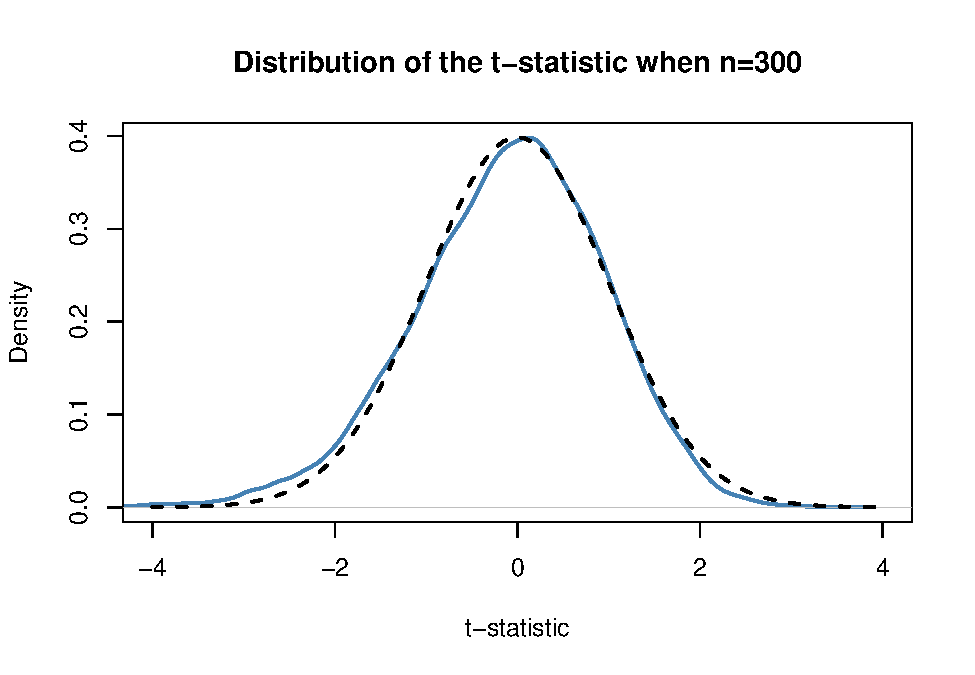
\includegraphics{URFITE_files/figure-latex/unnamed-chunk-55-1.pdf}

Judging from the plot, the normal approximation works reasonably well
for the chosen sample size. This normal approximation has already been
used in the definition of the \(p\)-value, see \eqref{eq:tstat}.

\subsection*{Hypothesis Testing with a Prespecified Significance
Level}\label{hypothesis-testing-with-a-prespecified-significance-level}
\addcontentsline{toc}{subsection}{Hypothesis Testing with a Prespecified
Significance Level}

Key Concept 3.5

The Terminology of Hypothesis Testing

In hypothesis testing, two types of mistakes are possible:

\begin{enumerate}
\def\labelenumi{\arabic{enumi}.}
\item
  The null hypothesis \emph{is} rejected although it is true
  (\(\alpha\)-error / type-I-error)
\item
  The null hypothesis \emph{is not} rejected although it is false
  (\(\beta\)-error / type-II-error)
\end{enumerate}

The significance level of the test is the probability to commit a
type-I-error we are willing to accept in advance. E.g. using a
prespecified significance level of \(0.05\), we reject the null
hypothesis if and only if the \(p\)-value is less than \(0.05\). The
significance level is chosen before the test is conducted.

An equivalent procedure is to reject the null hypothesis if the test
statistic observed is, in absolute value terms, larger than the critical
value of the test statistic. The critical value is determined by the
significance level chosen and defines two disjoint sets of values which
are called acceptance region and rejection region. The acceptance region
contains all values of the test statistic for which the test does not
reject while the rejection region contains all the values for which the
test does reject.

The \(p\)-value is the probability that, in repeated sampling under the
same conditions, meaning i.i.d. sampling, the same null hypothesis and
the same sample size, a test statistic is observed that provides just as
much evidence against the null hypothesis as the test statistic actually
observed.

The actual probability that the test rejects the true null hypothesis is
called the size of the test. In an ideal setting, the size does not
exceed the significance level.

The probability that the test correctly rejects a false null hypothesis
is called power.

Reconsider \texttt{pvalue} computed further above:

\begin{Shaded}
\begin{Highlighting}[]
\CommentTok{# check whether p-value < 0.05}
\NormalTok{pvalue }\OperatorTok{<}\StringTok{ }\FloatTok{0.05}
\end{Highlighting}
\end{Shaded}

\begin{verbatim}
## [1] FALSE
\end{verbatim}

The condition is not fulfilled so we do not reject the null hypotheis
(remember that the null hypothesis is true in this example).

When working with a \(t\)-statistic instead, it is equivalent to apply
the following rule:

\[ \text{Reject } H_0 \text{ if } \lvert t^{act} \rvert > 1.96 \]

We reject the null hypothesis at the significance level of \(5\%\) if
the computed \(t\)-statistic lies beyond the critical value of 1.96 in
absolute value terms. \(1.96\) is the \(0.05\)-quantile of the standard
normal distribution.

\begin{Shaded}
\begin{Highlighting}[]
\CommentTok{# check the critical value}
\KeywordTok{qnorm}\NormalTok{(}\DataTypeTok{p =} \FloatTok{0.05}\NormalTok{)}
\end{Highlighting}
\end{Shaded}

\begin{verbatim}
## [1] -1.644854
\end{verbatim}

\begin{Shaded}
\begin{Highlighting}[]
\CommentTok{# check whether the null is rejected using the t-statistic computed further above}
\KeywordTok{abs}\NormalTok{(tstatistic) }\OperatorTok{>}\StringTok{ }\FloatTok{1.96}
\end{Highlighting}
\end{Shaded}

\begin{verbatim}
## [1] FALSE
\end{verbatim}

As when using the \(p\)-value, we cannot reject the null hypothesis
using the corresponding \(t\)-statistic. Key Concept 3.6 summarizes the
procedure of performing a two-sided hypothesis about the population mean
\(E(Y)\).

Key Concept 3.6

Testing the Hypothesis \(E(Y) = \mu_{Y,0}\) Against the Alternative
\(E(Y) \neq \mu_{Y,0}\)

\begin{enumerate}
\def\labelenumi{\arabic{enumi}.}
\item
  Estimate \(\mu_{Y}\) using \(\overline{Y}\) and compute the standard
  error of \(\overline{Y}\), \(SE(\overline{Y})\).
\item
  Compute the \(t\)-statistic.
\item
  Compute the \(p\)-value and reject the null hypothesis at the \(5\%\)
  level of significance if the \(p\)-value is smaller than \(0.05\) or
  equivalently, if
\end{enumerate}

\[ \left\lvert t^{act} \right\rvert > 1.96. \]

\subsection*{One-sided Alternatives}\label{one-sided-alternatives}
\addcontentsline{toc}{subsection}{One-sided Alternatives}

Sometimes we are interested in finding evidence that the mean is bigger
or smaller than the some value hypothesized under the null. One can come
up with many examples here but, to stick to the book, take the presumed
wage differential between good and less educated working individuals.
Since we hope that this differential exists, a relevant alternative (to
the null hypothesis that there is no wage differential) is that good
educated individuals earn more, i.e.~that the average hourly wage for
this group, \(\mu_Y\) is \emph{bigger} than \(\mu_{Y,0}\) the know
average wage of less educated workers.

This is an example of a \emph{right-sided test} and the hypotheses pair
is chosen as

\[ H_0: \mu_Y = \mu_{Y,0} \ \ \text{vs} \ \ H_1: \mu_Y > \mu_{Y,0}. \]

We reject the null hypothesis if the computed test-statistic is larger
than the critical value \(1.64\), the \(0.95\)-quantile of the
\(N(0,1)\) distribution. This ensures that \(1-0.95=5\%\) probability
mass remains in the area to the right of the critical value. Similar as
before we can visualize this in R using the function \texttt{polygon()}.

\begin{Shaded}
\begin{Highlighting}[]
\CommentTok{# plot the standard normal density on the domain [-4,4]}
\KeywordTok{curve}\NormalTok{(}\KeywordTok{dnorm}\NormalTok{(x),}
      \DataTypeTok{xlim =} \KeywordTok{c}\NormalTok{(}\OperatorTok{-}\DecValTok{4}\NormalTok{,}\DecValTok{4}\NormalTok{),}
      \DataTypeTok{main =} \StringTok{'Rejection Region of a Right-Sided Test'}\NormalTok{,}
      \DataTypeTok{yaxs =} \StringTok{'i'}\NormalTok{,}
      \DataTypeTok{xlab =} \StringTok{'t-statistic'}\NormalTok{,}
      \DataTypeTok{ylab =} \StringTok{''}\NormalTok{,}
      \DataTypeTok{lwd =} \DecValTok{2}\NormalTok{,}
      \DataTypeTok{axes =} \StringTok{'F'}
\NormalTok{)}

\CommentTok{# add x-axis}
\KeywordTok{axis}\NormalTok{(}\DecValTok{1}\NormalTok{, }
     \DataTypeTok{at =} \KeywordTok{c}\NormalTok{(}\OperatorTok{-}\DecValTok{4}\NormalTok{,}\DecValTok{0}\NormalTok{,}\FloatTok{1.64}\NormalTok{,}\DecValTok{4}\NormalTok{), }
     \DataTypeTok{padj =} \FloatTok{0.5}\NormalTok{,}
     \DataTypeTok{labels =} \KeywordTok{c}\NormalTok{(}\StringTok{''}\NormalTok{,}\DecValTok{0}\NormalTok{,}\KeywordTok{expression}\NormalTok{(Phi}\OperatorTok{^-}\DecValTok{1}\OperatorTok{~}\NormalTok{(.}\DecValTok{95}\NormalTok{)}\OperatorTok{==}\FloatTok{1.64}\NormalTok{),}\StringTok{''}\NormalTok{)}
\NormalTok{)}

\CommentTok{# shade rejection region in right tail}
\KeywordTok{polygon}\NormalTok{(}\DataTypeTok{x =} \KeywordTok{c}\NormalTok{(}\FloatTok{1.64}\NormalTok{, }\KeywordTok{seq}\NormalTok{(}\FloatTok{1.64}\NormalTok{, }\DecValTok{4}\NormalTok{, }\FloatTok{0.01}\NormalTok{), }\DecValTok{4}\NormalTok{),}
        \DataTypeTok{y =} \KeywordTok{c}\NormalTok{(}\DecValTok{0}\NormalTok{, }\KeywordTok{dnorm}\NormalTok{(}\KeywordTok{seq}\NormalTok{(}\FloatTok{1.64}\NormalTok{, }\DecValTok{4}\NormalTok{, }\FloatTok{0.01}\NormalTok{)), }\DecValTok{0}\NormalTok{), }
        \DataTypeTok{col =} \StringTok{'darkred'}
\NormalTok{)}
\end{Highlighting}
\end{Shaded}

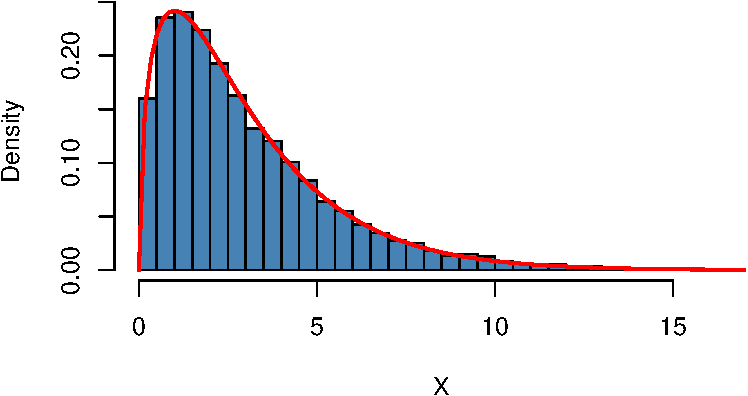
\includegraphics{URFITE_files/figure-latex/unnamed-chunk-58-1.pdf}

In an analogously manner for the \emph{left-sided test} we have

\[ H_0: \mu_Y = \mu_{Y,0} \ \ \text{vs.} \ \ H_1: \mu_Y < \mu_{Y,0}. \]

The null is rejected if the observed test statistic falls short of the
critical value which, for a test at the \(0.05\) level of significance,
is given by \(-1.64\), the \(0.05\)-quantile of the \(N(0,1)\)
distribution. \(5\%\) probability mass lies to the left of the critical
value.

It is straight forward to adapt the code chunk above to the case of a
left-sided test. We only have to fiddle with the color shading and the
tick marks.

\begin{Shaded}
\begin{Highlighting}[]
\CommentTok{# plot the standard normal density on the domain [-4,4]}
\KeywordTok{curve}\NormalTok{(}\KeywordTok{dnorm}\NormalTok{(x),}
      \DataTypeTok{xlim =} \KeywordTok{c}\NormalTok{(}\OperatorTok{-}\DecValTok{4}\NormalTok{,}\DecValTok{4}\NormalTok{),}
      \DataTypeTok{main =} \StringTok{'Rejection Region of a Left-Sided Test'}\NormalTok{,}
      \DataTypeTok{yaxs =} \StringTok{'i'}\NormalTok{,}
      \DataTypeTok{xlab =} \StringTok{'t-statistic'}\NormalTok{,}
      \DataTypeTok{ylab =} \StringTok{''}\NormalTok{,}
      \DataTypeTok{lwd =} \DecValTok{2}\NormalTok{,}
      \DataTypeTok{axes =} \StringTok{'F'}
\NormalTok{)}

\CommentTok{# add x-axis}
\KeywordTok{axis}\NormalTok{(}\DecValTok{1}\NormalTok{, }
     \DataTypeTok{at =} \KeywordTok{c}\NormalTok{(}\OperatorTok{-}\DecValTok{4}\NormalTok{,}\DecValTok{0}\NormalTok{,}\OperatorTok{-}\FloatTok{1.64}\NormalTok{,}\DecValTok{4}\NormalTok{), }
     \DataTypeTok{padj =} \FloatTok{0.5}\NormalTok{,}
     \DataTypeTok{labels =} \KeywordTok{c}\NormalTok{(}\StringTok{''}\NormalTok{,}\DecValTok{0}\NormalTok{,}\KeywordTok{expression}\NormalTok{(Phi}\OperatorTok{^-}\DecValTok{1}\OperatorTok{~}\NormalTok{(.}\DecValTok{05}\NormalTok{)}\OperatorTok{==-}\FloatTok{1.64}\NormalTok{),}\StringTok{''}\NormalTok{)}
\NormalTok{)}

\CommentTok{# shade rejection region in right tail}
\KeywordTok{polygon}\NormalTok{(}\DataTypeTok{x =} \KeywordTok{c}\NormalTok{(}\OperatorTok{-}\DecValTok{4}\NormalTok{, }\KeywordTok{seq}\NormalTok{(}\OperatorTok{-}\DecValTok{4}\NormalTok{, }\OperatorTok{-}\FloatTok{1.64}\NormalTok{, }\FloatTok{0.01}\NormalTok{), }\OperatorTok{-}\FloatTok{1.64}\NormalTok{),}
        \DataTypeTok{y =} \KeywordTok{c}\NormalTok{(}\DecValTok{0}\NormalTok{, }\KeywordTok{dnorm}\NormalTok{(}\KeywordTok{seq}\NormalTok{(}\OperatorTok{-}\DecValTok{4}\NormalTok{, }\OperatorTok{-}\FloatTok{1.64}\NormalTok{, }\FloatTok{0.01}\NormalTok{)), }\DecValTok{0}\NormalTok{), }
        \DataTypeTok{col =} \StringTok{'darkred'}
\NormalTok{)}
\end{Highlighting}
\end{Shaded}

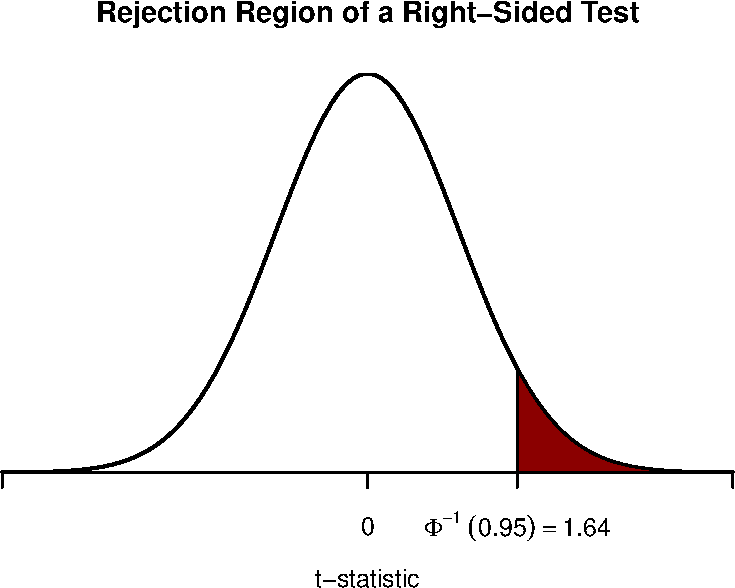
\includegraphics{URFITE_files/figure-latex/unnamed-chunk-59-1.pdf}

\section{Confidence intervals for the Population
Mean}\label{confidence-intervals-for-the-population-mean}

As stressed before, we will never estimate the exact value of a the
population mean of \(Y\) using a random sample. However, we can compute
confidence intervals for the population mean. In general, a confidence
interval for a unkown parameter is a set of values that contains the
true parameter with a prespecified probability, the confidence level.
Confidence intervals are computed using the information available in the
sample. Since this information is the result of a random process,
confidence intervals are random variables themselves.

Key Concept 3.7 shows how to compute confidence intervals for the
unknown population mean \(E(Y)\).

Key Concept 3.6

Confidence Intervals for the Population Mean

A \(95\%\) confidence interval for \(\mu_Y\) is a random variable that
contains the true \(\mu_Y\) in \(95\%\) of all possible random samples.
When \(n\) is large we can use the normal approximation. Then, \(99\%\),
\(95\%\), \(90\%\) confidence intervals are

\begin{align}
&99\%\text{ confidence interval for } \mu_Y = \left\{ \overline{Y} \pm 2.58 \times SE(\overline{Y}) \right\}. \\
&95\%\text{ confidence interval for } \mu_Y = \left\{ \overline{Y} \pm 1.96 \times SE(\overline{Y}) \right\}. \\
&90\%\text{ confidence interval for } \mu_Y = \left\{ \overline{Y} \pm 1.64 \times SE(\overline{Y}) \right\}.
\end{align}

These confidence intervals are sets of null hypotheses we cannot reject
in a two-sided hypothesis test at the given level of confidence.

Now consider the following statements.

\begin{enumerate}
\def\labelenumi{\arabic{enumi}.}
\item
  The interval
  \[ \left\{ \overline{Y} \pm 1.96 \times SE(\overline{Y}) \right\} \]
  covers the true value of \(\mu_Y\) with a probability of \(95\%\).
\item
  We have computed \(\overline{Y} = 5.1\) and \(SE(\overline{Y}=2.5\) so
  the interval
  \[ \left\{ 5.1  \pm 1.96 \times 2.5 \right\} = \left[0.2,10\right] \]
  covers the true value of \(\mu_Y\) with a probability of \(95\%\).
\end{enumerate}

While 1. is right (this is exactly in line with the definition above),
2. is completely wrong and none of Your lecturers wants to read such a
sentence in a term paper, written exam or similar, believe us. The
difference is that, while 1. is the definition of a random variable, 2.
is one possible \emph{outcome} of this random variable so there is no
meaning in making any probabilistic statement about it. Either the
computed interval \emph{does cover} \(\mu_Y\) or it \emph{does not}!

In R, testing hypothesis about the mean of a population on the basis of
a random sample is very easy due to functions like \texttt{t.test()}
from the stats package. It procudes an object of type list. Luckily, one
of the most simple ways to use \texttt{t.test()} is when You want to
obtain a \(95\%\) confidence interval for some population mean. We start
by generating some random data and calling \texttt{t.test()} in
conjunction with \texttt{ls()} to obtain a breakdown of the output
components.

\begin{Shaded}
\begin{Highlighting}[]
\CommentTok{# set random seed}
\KeywordTok{set.seed}\NormalTok{(}\DecValTok{1}\NormalTok{)}

\CommentTok{# generate some sample data}
\NormalTok{sampledata <-}\StringTok{ }\KeywordTok{rnorm}\NormalTok{(}\DecValTok{100}\NormalTok{,}\DecValTok{10}\NormalTok{,}\DecValTok{10}\NormalTok{)}

\CommentTok{# checke type}
\KeywordTok{typeof}\NormalTok{(}\KeywordTok{t.test}\NormalTok{(sampledata))}
\end{Highlighting}
\end{Shaded}

\begin{verbatim}
## [1] "list"
\end{verbatim}

\begin{Shaded}
\begin{Highlighting}[]
\CommentTok{# display list elements produced by t.test}
\KeywordTok{ls}\NormalTok{(}
  \KeywordTok{t.test}\NormalTok{(sampledata)}
\NormalTok{)}
\end{Highlighting}
\end{Shaded}

\begin{verbatim}
## [1] "alternative" "conf.int"    "data.name"   "estimate"    "method"     
## [6] "null.value"  "p.value"     "parameter"   "statistic"
\end{verbatim}

Though we find that many items are reported, at the moment we are
interested in computing a \(95\%\) confidence set for the mean.

\begin{Shaded}
\begin{Highlighting}[]
\KeywordTok{t.test}\NormalTok{(sampledata)}\OperatorTok{$}\StringTok{"conf.int"}
\end{Highlighting}
\end{Shaded}

\begin{verbatim}
## [1]  9.306651 12.871096
## attr(,"conf.level")
## [1] 0.95
\end{verbatim}

This tells us that the \(95\%\) confidence interval is

\[ \left[9.31, 12.87\right]. \]

In this example, the computed interval does cover the true \(\mu_Y\)
which we know to be \(10\).

Let us have a look at the whole standard output produced by
\texttt{t.test()}.

\begin{Shaded}
\begin{Highlighting}[]
\KeywordTok{t.test}\NormalTok{(sampledata)}
\end{Highlighting}
\end{Shaded}

\begin{verbatim}
## 
##  One Sample t-test
## 
## data:  sampledata
## t = 12.346, df = 99, p-value < 2.2e-16
## alternative hypothesis: true mean is not equal to 0
## 95 percent confidence interval:
##   9.306651 12.871096
## sample estimates:
## mean of x 
##  11.08887
\end{verbatim}

We see that \texttt{t.test()} not only computes a \(95\%\) confidence
interval but automatically conducts a two-sided significance test of the
hypothesis \(H_0: \mu_Y = 0\) at the level of \(5\%\) and reports
relevant parameters thereof: the alternative hypothesis, the estimated
mean, the resulting \(t\)-statistic, the degrees of freedom of the
underlying \(t\) distribution (\texttt{t.test()} does not perform the
normal approximation) and the corresponding \(p\)-value. Very
convenient!

In this example, we come to the conclusion that the population mean
\emph{is not} significantly different from \(0\) at the level of \(5\%\)
(which is correct), since \(\mu_Y = 0\) is element of the \(95\%\)
confidence interval

\[ 0 \in \left[-0.27,0.12\right]. \] We come to an equivalent result
when using the \(p\)-value rejection rule:

\[ p = 0.456 > 0.05 \]

\section{Comparing Means from Different
Populations}\label{comparing-means-from-different-populations}

Suppose You are interested in the means of two different populations,
denote them \(\mu_1\) and \(\mu_2\). More specifically You are
interested whether these population means are different from each other
and plan an using a hypothesis test to verifiy this on the basis of
independent sample data from both populations. A suitable pair of
hypotheses then is

\begin{equation}
H_0: \mu_1 - \mu_2 = d_0 \ \ \text{vs.} \ \ H_1: \mu_1 - \mu_2 \neq d_0 \label{eq:hypmeans}
\end{equation}

where \(d_0\) denotes the hypothesized difference in means. The book
teaches us that \(H_0\) can be tested with the \(t\)-statistic

\begin{equation}
t=\frac{(\overline{Y}_1 - \overline{Y}_2) - d_0}{SE(\overline{Y}_1 - \overline{Y}_2)} \label{eq:tstatmeans}
\end{equation}

where

\begin{equation}
SE(\overline{Y}_1 - \overline{Y}_2) = \sqrt{\frac{s_1^2}{n_1} + \frac{s_2^2}{n_2}}.
\end{equation}

This is called a two sample \(t\)-test. For large \(n_1\) and \(n_2\),
\eqref{eq:tstatmeans} is standard normal distributed under the null
hypothesis. Anlog to the simple \(t\)-test we can compute confidence
intervals for the true difference in population means:

\[ (\overline{Y}_1 - \overline{Y}_2) \pm 1.96 \times SE(\overline{Y}_1 - \overline{Y}_2) \]

is a \(95\%\) confidence interval for \(d\). In R, Hypotheses as in
\eqref{eq:hypmeans} can be tested with \texttt{t.test()}, too. Note that
\texttt{t.test()} chooses \(d_0 = 0\) by default. This can be changed by
setting the argument \texttt{mu} accordingly.

\begin{Shaded}
\begin{Highlighting}[]
\CommentTok{# set random seed}
\KeywordTok{set.seed}\NormalTok{(}\DecValTok{1}\NormalTok{)}

\CommentTok{# draw data from two different populations with equal mean}
\NormalTok{sample_pop1 <-}\StringTok{ }\KeywordTok{rnorm}\NormalTok{(}\DecValTok{100}\NormalTok{, }\DecValTok{10}\NormalTok{, }\DecValTok{10}\NormalTok{)}
\NormalTok{sample_pop2 <-}\StringTok{ }\KeywordTok{rnorm}\NormalTok{(}\DecValTok{100}\NormalTok{, }\DecValTok{10}\NormalTok{, }\DecValTok{20}\NormalTok{)}

\CommentTok{# perform a two sample t-test}
\KeywordTok{t.test}\NormalTok{(sample_pop1, sample_pop2)}
\end{Highlighting}
\end{Shaded}

\begin{verbatim}
## 
##  Welch Two Sample t-test
## 
## data:  sample_pop1 and sample_pop2
## t = 0.872, df = 140.52, p-value = 0.3847
## alternative hypothesis: true difference in means is not equal to 0
## 95 percent confidence interval:
##  -2.338012  6.028083
## sample estimates:
## mean of x mean of y 
## 11.088874  9.243838
\end{verbatim}

We find that the two sample \(t\)-test does not reject the (true) null
hypothesis that \(d_0 = 0\).

\section{An Application to the Gender Gap of
Earnings}\label{an-application-to-the-gender-gap-of-earnings}

In this section discusses how to reproduce the results presented in the
box `\emph{The Gender Gap of Earnings of College Graduates in the United
States}' in the book.

In order to reproduce table 3.1 You need to download the replication
data which is hosted by Pearson and can be found and downloaded
\href{http://wps.aw.com/aw_stock_ie_3/178/45691/11696965.cw/index.html}{here}.
Download the data for chapter three as an excel spreadsheet
(cps\_ch3.xlsx). This data set contains data that ranges from \(1992\)
to \(2008\) and earnings are reported in prices of \(2008\). There are
several ways to import the .xlsx-files into R. Our suggestion is the
function \texttt{read\_excel()} from the readxl package. The package is
not part of R's standard distribution and has to be installed manually.

\begin{Shaded}
\begin{Highlighting}[]
\CommentTok{# install and load the readxl package}
\NormalTok{## install.packages('readxl')}
\KeywordTok{library}\NormalTok{(readxl)}
\end{Highlighting}
\end{Shaded}

You are now ready to import the data set. Make sure You use the correct
path to the downloaded file! In our example, the file is saved in a
subfolder (data) of the working directory. If You are not sure what Your
current working directory is, use \texttt{getwd()}, see also
\texttt{?getwd()}. This will give You the path that points to the place
R is currently looking for files.

\begin{Shaded}
\begin{Highlighting}[]
\CommentTok{# import the data into R}
\NormalTok{cps <-}\StringTok{ }\KeywordTok{read_excel}\NormalTok{(}\DataTypeTok{path =} \StringTok{'data/cps_ch3.xlsx'}\NormalTok{)}
\end{Highlighting}
\end{Shaded}

Next, install and load the package dyplr. This package provides some
handy functions that simplify data wrangling a lot. It makes use of the
\texttt{\%\textgreater{}\%} operator.

\BeginKnitrBlock{rmdknit}
In general, the aim of pipe operators is to increase readability of
written code. The pipe operator \%\textgreater{}\%, also known as
magrittr, is relatively new to R. It was originally introduced with the
package magrittr but is available for several R packages. The most
prominent ones are plotly and dplyr. See the following
\href{https://cran.r-project.org/web/packages/magrittr/vignettes/magrittr.html}{link}
for more on the magrittr package.

The basic idea is to simplify a sequece of function calls by chaining
them. 1:10 \%\textgreater{}\% mean\\
\# {[}1{]} 5.5\\
 \# is equivalent to mean(1:10)\\
\# {[}1{]} 5.5
\EndKnitrBlock{rmdknit}

\begin{Shaded}
\begin{Highlighting}[]
\CommentTok{# install and load the dplyr package}
\NormalTok{## install.packages('dplyr')}
\KeywordTok{library}\NormalTok{(}\StringTok{'dplyr'}\NormalTok{)}
\end{Highlighting}
\end{Shaded}

First, get an overview over the data set. Next, use
\texttt{\%\textgreater{}\%} and some functions from the \texttt{dplyr}
package to group the observations by gender and year and compute
descriptive statistics for both groups.

\begin{Shaded}
\begin{Highlighting}[]
\CommentTok{# Get an overview of the data structure}
\KeywordTok{head}\NormalTok{(cps)}
\end{Highlighting}
\end{Shaded}

\begin{verbatim}
## # A tibble: 6 x 3
##   a_sex  year    ahe08
##   <dbl> <dbl>    <dbl>
## 1     1  1992 17.16203
## 2     1  1992 15.33856
## 3     1  1992 22.94229
## 4     2  1992 13.28334
## 5     1  1992 22.12292
## 6     2  1992 12.16761
\end{verbatim}

\begin{Shaded}
\begin{Highlighting}[]
\CommentTok{# group data by gender and year and compute the mean, standard deviation}
\CommentTok{# and number of observations for each group}
\NormalTok{avgs <-}\StringTok{ }\NormalTok{cps }\OperatorTok\StringTok{ }
\StringTok{        }\KeywordTok{group_by}\NormalTok{(a_sex, year) }\OperatorTok\StringTok{ }
\StringTok{        }\KeywordTok{summarise}\NormalTok{(}\KeywordTok{mean}\NormalTok{(ahe08), }
                  \KeywordTok{sd}\NormalTok{(ahe08), }
                  \KeywordTok{n}\NormalTok{()}
\NormalTok{                  )}

\CommentTok{# print results to the console}
\KeywordTok{print}\NormalTok{(avgs)}
\end{Highlighting}
\end{Shaded}

\begin{verbatim}
## # A tibble: 10 x 5
## # Groups:   a_sex [?]
##    a_sex  year `mean(ahe08)` `sd(ahe08)` `n()`
##    <dbl> <dbl>         <dbl>       <dbl> <int>
##  1     1  1992      23.27382   10.172081  1594
##  2     1  1996      22.47544   10.103141  1379
##  3     1  2000      24.88314   11.599727  1303
##  4     1  2004      25.12169   12.008435  1894
##  5     1  2008      24.97840   11.778632  1838
##  6     2  1992      20.04629    7.868418  1368
##  7     2  1996      18.98048    7.951608  1230
##  8     2  2000      20.73938    9.359327  1181
##  9     2  2004      21.02373    9.363071  1735
## 10     2  2008      20.87478    9.657140  1871
\end{verbatim}

With the pipe operator \texttt{\%\textgreater{}\%} we simply chain
different R functions that produce compatible input and ouput. In the
code above, we take the dataset \texttt{cps} and use it as an input for
the function \texttt{group\_by()}. The output of \texttt{group\_by} is
subsequently used as an input for \texttt{summarise()} and so forth.

Now that we have computed the statistics of interest for both genders,
we can investigate how the gap in earnings between both groups evolves
over time.

\begin{Shaded}
\begin{Highlighting}[]
\CommentTok{# split the data set by gender}
\NormalTok{male <-}\StringTok{ }\NormalTok{avgs }\OperatorTok\StringTok{ }\KeywordTok{filter}\NormalTok{(a_sex }\OperatorTok{==}\StringTok{ }\DecValTok{1}\NormalTok{) }
\NormalTok{female <-}\StringTok{ }\NormalTok{avgs }\OperatorTok\StringTok{ }\KeywordTok{filter}\NormalTok{(a_sex }\OperatorTok{==}\StringTok{ }\DecValTok{2}\NormalTok{)}

\CommentTok{# Rename columns of both splits}
\KeywordTok{colnames}\NormalTok{(male)   <-}\StringTok{ }\KeywordTok{c}\NormalTok{(}\StringTok{"Sex"}\NormalTok{, }\StringTok{"Year"}\NormalTok{, }\StringTok{"Y_bar_m"}\NormalTok{, }\StringTok{"s_m"}\NormalTok{, }\StringTok{"n_m"}\NormalTok{)}
\KeywordTok{colnames}\NormalTok{(female) <-}\StringTok{ }\KeywordTok{c}\NormalTok{(}\StringTok{"Sex"}\NormalTok{, }\StringTok{"Year"}\NormalTok{, }\StringTok{"Y_bar_f"}\NormalTok{, }\StringTok{"s_f"}\NormalTok{, }\StringTok{"n_f"}\NormalTok{)}

\CommentTok{# Estimate Gender gaps, compute standard errors and confidence intervals for all dates}
\NormalTok{gap <-}\StringTok{ }\NormalTok{male}\OperatorTok{$}\NormalTok{Y_bar_m }\OperatorTok{-}\StringTok{ }\NormalTok{female}\OperatorTok{$}\NormalTok{Y_bar_f}

\NormalTok{gap_se <-}\StringTok{ }\KeywordTok{sqrt}\NormalTok{(male}\OperatorTok{$}\NormalTok{s_m}\OperatorTok{^}\DecValTok{2} \OperatorTok{/}\StringTok{ }\NormalTok{male}\OperatorTok{$}\NormalTok{n_m }\OperatorTok{+}\StringTok{ }\NormalTok{female}\OperatorTok{$}\NormalTok{s_f}\OperatorTok{^}\DecValTok{2} \OperatorTok{/}\StringTok{ }\NormalTok{female}\OperatorTok{$}\NormalTok{n_f)}

\NormalTok{gap_ci_l <-}\StringTok{ }\NormalTok{gap }\OperatorTok{-}\StringTok{ }\FloatTok{1.96} \OperatorTok{*}\StringTok{ }\NormalTok{gap_se}

\NormalTok{gap_ci_u <-}\StringTok{ }\NormalTok{gap }\OperatorTok{+}\StringTok{ }\FloatTok{1.96} \OperatorTok{*}\StringTok{ }\NormalTok{gap_se}

\NormalTok{result <-}\StringTok{ }\KeywordTok{cbind}\NormalTok{(male[,}\OperatorTok{-}\DecValTok{1}\NormalTok{], female[,}\OperatorTok{-}\NormalTok{(}\DecValTok{1}\OperatorTok{:}\DecValTok{2}\NormalTok{)], gap, gap_se, gap_ci_l, gap_ci_u)}

\CommentTok{# print results to the console}
\KeywordTok{print}\NormalTok{(result, }\DataTypeTok{digits =} \DecValTok{3}\NormalTok{)}
\end{Highlighting}
\end{Shaded}

\begin{verbatim}
##   Year Y_bar_m  s_m  n_m Y_bar_f  s_f  n_f  gap gap_se gap_ci_l gap_ci_u
## 1 1992    23.3 10.2 1594    20.0 7.87 1368 3.23  0.332     2.58     3.88
## 2 1996    22.5 10.1 1379    19.0 7.95 1230 3.49  0.354     2.80     4.19
## 3 2000    24.9 11.6 1303    20.7 9.36 1181 4.14  0.421     3.32     4.97
## 4 2004    25.1 12.0 1894    21.0 9.36 1735 4.10  0.356     3.40     4.80
## 5 2008    25.0 11.8 1838    20.9 9.66 1871 4.10  0.354     3.41     4.80
\end{verbatim}

We observe virtually the same results as the ones presented in the book.
the computed statistics suggest that there \emph{is} a gender gap in
earnings. Note that we can reject the null hypothesis that the gap is
zero for all periodes. Further, estimates of the gap and bounds of the
95\% confidence intervals indicate that the gap has been quite stable
over the recent past.

\section{Scatterplots, Sample Covariance and Sample
Correlation}\label{scatterplots-sample-covariance-and-sample-correlation}

A scatterplot represents two dimensional data, for example \(n\)
observation on \(X_i\) and \(Y_i\), by points in a cartesian coordinate
system. It is very easy to generate scatterplots using the
\texttt{plot()} function in R. Let's generate some fictional data on age
and earnings of workers and plot it.

\begin{Shaded}
\begin{Highlighting}[]
\CommentTok{# set random seed}
\KeywordTok{set.seed}\NormalTok{(}\DecValTok{123}\NormalTok{)}

\CommentTok{# generate data set}
\NormalTok{X <-}\StringTok{ }\KeywordTok{runif}\NormalTok{(}\DataTypeTok{n =} \DecValTok{100}\NormalTok{, }
           \DataTypeTok{min =} \DecValTok{18}\NormalTok{, }
           \DataTypeTok{max =} \DecValTok{70}
\NormalTok{           )}
\NormalTok{Y <-}\StringTok{ }\NormalTok{X }\OperatorTok{+}\StringTok{ }\KeywordTok{rnorm}\NormalTok{(}\DataTypeTok{n=}\DecValTok{100}\NormalTok{, }\DecValTok{50}\NormalTok{, }\DecValTok{15}\NormalTok{)}

\CommentTok{# plot observations}
\KeywordTok{plot}\NormalTok{(X, }
\NormalTok{     Y, }
     \DataTypeTok{type =} \StringTok{"p"}\NormalTok{,}
     \DataTypeTok{main =} \StringTok{"A Scatterplot of X and Y"}\NormalTok{,}
     \DataTypeTok{xlab =} \StringTok{"Age"}\NormalTok{,}
     \DataTypeTok{ylab =} \StringTok{"Earnings"}\NormalTok{,}
     \DataTypeTok{col =} \StringTok{"steelblue"}\NormalTok{,}
     \DataTypeTok{pch =} \DecValTok{19}
\NormalTok{     )}
\end{Highlighting}
\end{Shaded}

\begin{center}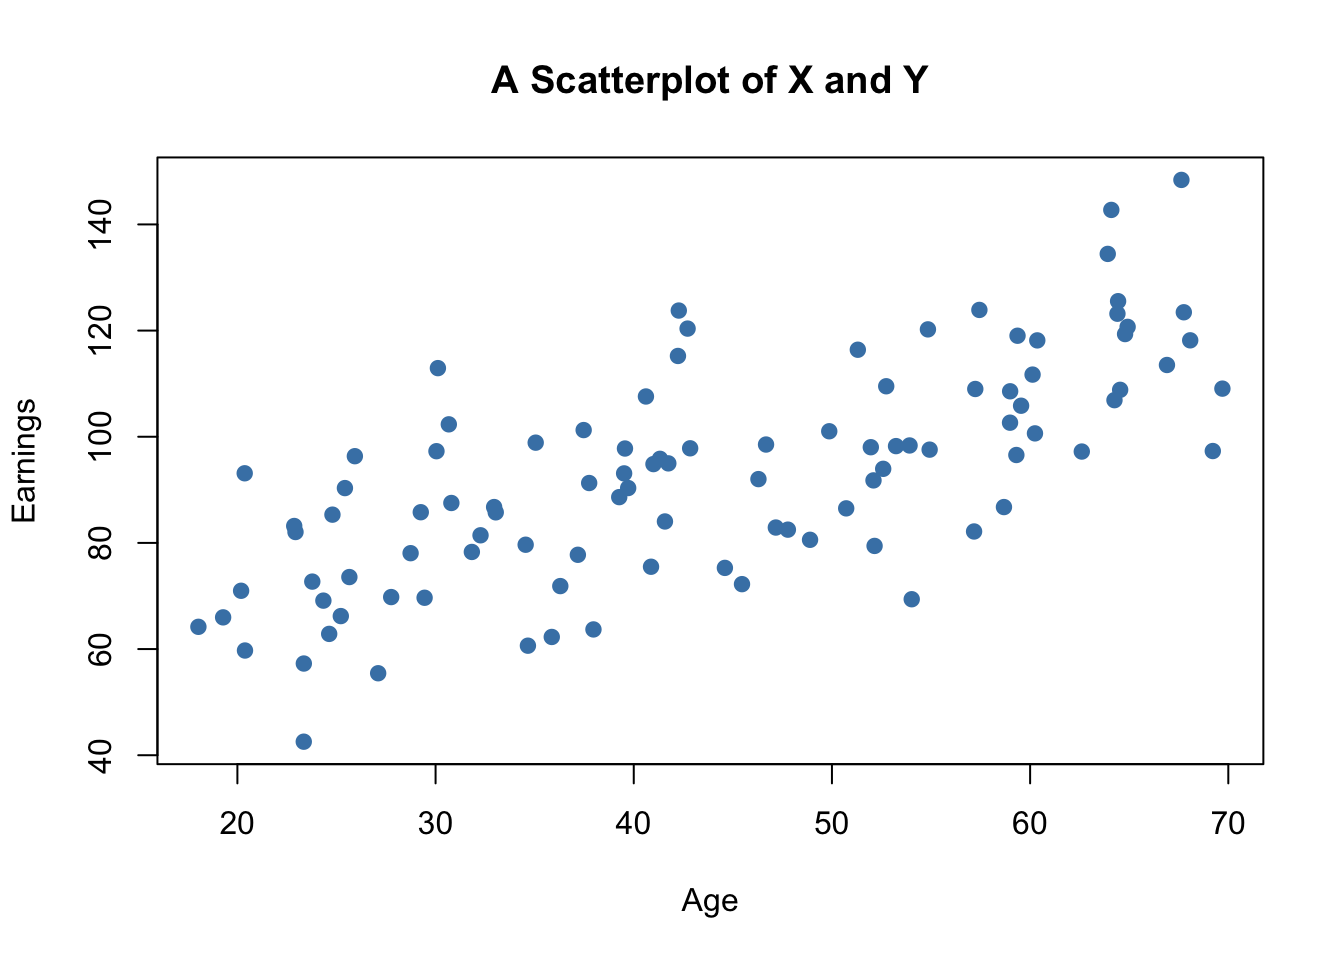
\includegraphics{URFITE_files/figure-latex/unnamed-chunk-69-1} \end{center}

The plot shows positive correlation between age and earnings. This in
line with the assumption that older workers earn more than those that
the joined the working population recently.

\subsubsection*{Sample Covariance and
Correlation}\label{sample-covariance-and-correlation}
\addcontentsline{toc}{subsubsection}{Sample Covariance and Correlation}

By now You should be familiar with the concepts of variance and
covariance. If not, we recommend You to work Your way through chapter 2
of the book (again).

As for the variance, covariance and correlation of two variables are
properties that relate to the (unknown) joint probability distribution
of these variable. Just as the individual population variances of both
variables, we can estimate covariance and correlation by means of
suitable estimators using a random sample \((X_i,Y_i)\),
\(i=1,\dots,n\).

The sample covariance

\[ s_{XY} = \frac{1}{n-1} \sum_{i=1}^n (X_i - \overline{X})(Y_i - \overline{Y}) \]

is an estimator for the population variance of \(X\) and \(Y\) whereas
the sample correlation

\[ r_{XY} = \frac{s_{XY}}{s_Xs_Y} \] can be used to estimate the
population correlation, a standardized measure for the strength of the
linear relationship between \(X\) and \(Y\). See chapter 3.7 in the book
for a more detailed treatment of these estimators.

As for variance and standard deviation, these estimators are implemented
as R functions in the stats package. We can use them to estimate
population covariance and population correlation the fictional data on
age and earnings.

\begin{Shaded}
\begin{Highlighting}[]
\CommentTok{# compute sample covariance of X and Y}
\KeywordTok{cov}\NormalTok{(X,Y)}
\end{Highlighting}
\end{Shaded}

\begin{verbatim}
## [1] 213.934
\end{verbatim}

\begin{Shaded}
\begin{Highlighting}[]
\CommentTok{# compute sample correlation between X and Y}
\KeywordTok{cor}\NormalTok{(X,Y)}
\end{Highlighting}
\end{Shaded}

\begin{verbatim}
## [1] 0.706372
\end{verbatim}

\begin{Shaded}
\begin{Highlighting}[]
\CommentTok{# equivalent way to compute the sample correlation}
\KeywordTok{cov}\NormalTok{(X,Y)}\OperatorTok{/}\NormalTok{(}\KeywordTok{sd}\NormalTok{(X) }\OperatorTok{*}\StringTok{ }\KeywordTok{sd}\NormalTok{(Y))}
\end{Highlighting}
\end{Shaded}

\begin{verbatim}
## [1] 0.706372
\end{verbatim}

The estimates indicate that \(X\) and \(Y\) are moderately correlated.

The next code chunk uses the function \texttt{mvnorm()} from package
MASS to generate bivariate example data with different degree of
correlation.

\begin{Shaded}
\begin{Highlighting}[]
\KeywordTok{library}\NormalTok{(MASS)}

\CommentTok{# set random seed}
\KeywordTok{set.seed}\NormalTok{(}\DecValTok{1}\NormalTok{)}

\CommentTok{# positive correlation (0.81)}
\NormalTok{example1 <-}\StringTok{ }\KeywordTok{mvrnorm}\NormalTok{(}\DecValTok{100}\NormalTok{,}
                    \DataTypeTok{mu =} \KeywordTok{c}\NormalTok{(}\DecValTok{0}\NormalTok{,}\DecValTok{0}\NormalTok{), }
                    \DataTypeTok{Sigma =} \KeywordTok{matrix}\NormalTok{(}\KeywordTok{c}\NormalTok{(}\DecValTok{2}\NormalTok{,}\DecValTok{2}\NormalTok{,}\DecValTok{2}\NormalTok{,}\DecValTok{3}\NormalTok{), }\DataTypeTok{ncol =} \DecValTok{2}\NormalTok{),}
                    \DataTypeTok{empirical =} \OtherTok{TRUE}
\NormalTok{                    )}

\CommentTok{# negative correlation (-0.81)}
\NormalTok{example2 <-}\StringTok{ }\KeywordTok{mvrnorm}\NormalTok{(}\DecValTok{100}\NormalTok{,}
                    \DataTypeTok{mu =} \KeywordTok{c}\NormalTok{(}\DecValTok{0}\NormalTok{,}\DecValTok{0}\NormalTok{), }
                    \DataTypeTok{Sigma =} \KeywordTok{matrix}\NormalTok{(}\KeywordTok{c}\NormalTok{(}\DecValTok{2}\NormalTok{,}\OperatorTok{-}\DecValTok{2}\NormalTok{,}\OperatorTok{-}\DecValTok{2}\NormalTok{,}\DecValTok{3}\NormalTok{), }\DataTypeTok{ncol =} \DecValTok{2}\NormalTok{),}
                    \DataTypeTok{empirical =} \OtherTok{TRUE}
\NormalTok{                    )}

\CommentTok{# no correlation }
\NormalTok{example3 <-}\StringTok{ }\KeywordTok{mvrnorm}\NormalTok{(}\DecValTok{100}\NormalTok{,}
                    \DataTypeTok{mu =} \KeywordTok{c}\NormalTok{(}\DecValTok{0}\NormalTok{,}\DecValTok{0}\NormalTok{), }
                    \DataTypeTok{Sigma =} \KeywordTok{matrix}\NormalTok{(}\KeywordTok{c}\NormalTok{(}\DecValTok{1}\NormalTok{,}\DecValTok{0}\NormalTok{,}\DecValTok{0}\NormalTok{,}\DecValTok{1}\NormalTok{), }\DataTypeTok{ncol =} \DecValTok{2}\NormalTok{),}
                    \DataTypeTok{empirical =} \OtherTok{TRUE}
\NormalTok{                    )}

\CommentTok{# no correlation (quadratic relationship)}
\NormalTok{X <-}\StringTok{ }\KeywordTok{seq}\NormalTok{(}\OperatorTok{-}\DecValTok{3}\NormalTok{,}\DecValTok{3}\NormalTok{,}\FloatTok{0.01}\NormalTok{)}
\NormalTok{Y <-}\StringTok{ }\OperatorTok{-}\NormalTok{X}\OperatorTok{^}\DecValTok{2} \OperatorTok{+}\StringTok{ }\KeywordTok{rnorm}\NormalTok{(}\KeywordTok{length}\NormalTok{(X))}

\NormalTok{example4 <-}\StringTok{ }\KeywordTok{cbind}\NormalTok{(X,Y)}

\CommentTok{# estimate}

\NormalTok{## Plots}

\CommentTok{# divide plot area as 2-by-2 array}
\KeywordTok{par}\NormalTok{(}\DataTypeTok{mfrow=}\KeywordTok{c}\NormalTok{(}\DecValTok{2}\NormalTok{,}\DecValTok{2}\NormalTok{))}

\KeywordTok{plot}\NormalTok{(example1, }\DataTypeTok{col=}\StringTok{'steelblue'}\NormalTok{, }\DataTypeTok{pch=}\DecValTok{20}\NormalTok{, }\DataTypeTok{xlab =} \StringTok{'X'}\NormalTok{, }\DataTypeTok{ylab =} \StringTok{'Y'}\NormalTok{, }\DataTypeTok{main=}\StringTok{"Correlation = 0.81"}\NormalTok{)}
\KeywordTok{plot}\NormalTok{(example2, }\DataTypeTok{col=}\StringTok{'steelblue'}\NormalTok{, }\DataTypeTok{pch=}\DecValTok{20}\NormalTok{, }\DataTypeTok{xlab =} \StringTok{'X'}\NormalTok{, }\DataTypeTok{ylab =} \StringTok{'Y'}\NormalTok{, }\DataTypeTok{main=}\StringTok{"Correlation = -0.81"}\NormalTok{)}
\KeywordTok{plot}\NormalTok{(example3, }\DataTypeTok{col=}\StringTok{'steelblue'}\NormalTok{, }\DataTypeTok{pch=}\DecValTok{20}\NormalTok{, }\DataTypeTok{xlab =} \StringTok{'X'}\NormalTok{, }\DataTypeTok{ylab =} \StringTok{'Y'}\NormalTok{, }\DataTypeTok{main=}\StringTok{"Correlation = 0"}\NormalTok{)}
\KeywordTok{plot}\NormalTok{(example4, }\DataTypeTok{col=}\StringTok{'steelblue'}\NormalTok{, }\DataTypeTok{pch=}\DecValTok{20}\NormalTok{, }\DataTypeTok{xlab =} \StringTok{'X'}\NormalTok{, }\DataTypeTok{ylab =} \StringTok{'Y'}\NormalTok{, }\DataTypeTok{main=}\StringTok{"Correlation = 0"}\NormalTok{)}
\end{Highlighting}
\end{Shaded}

\begin{center}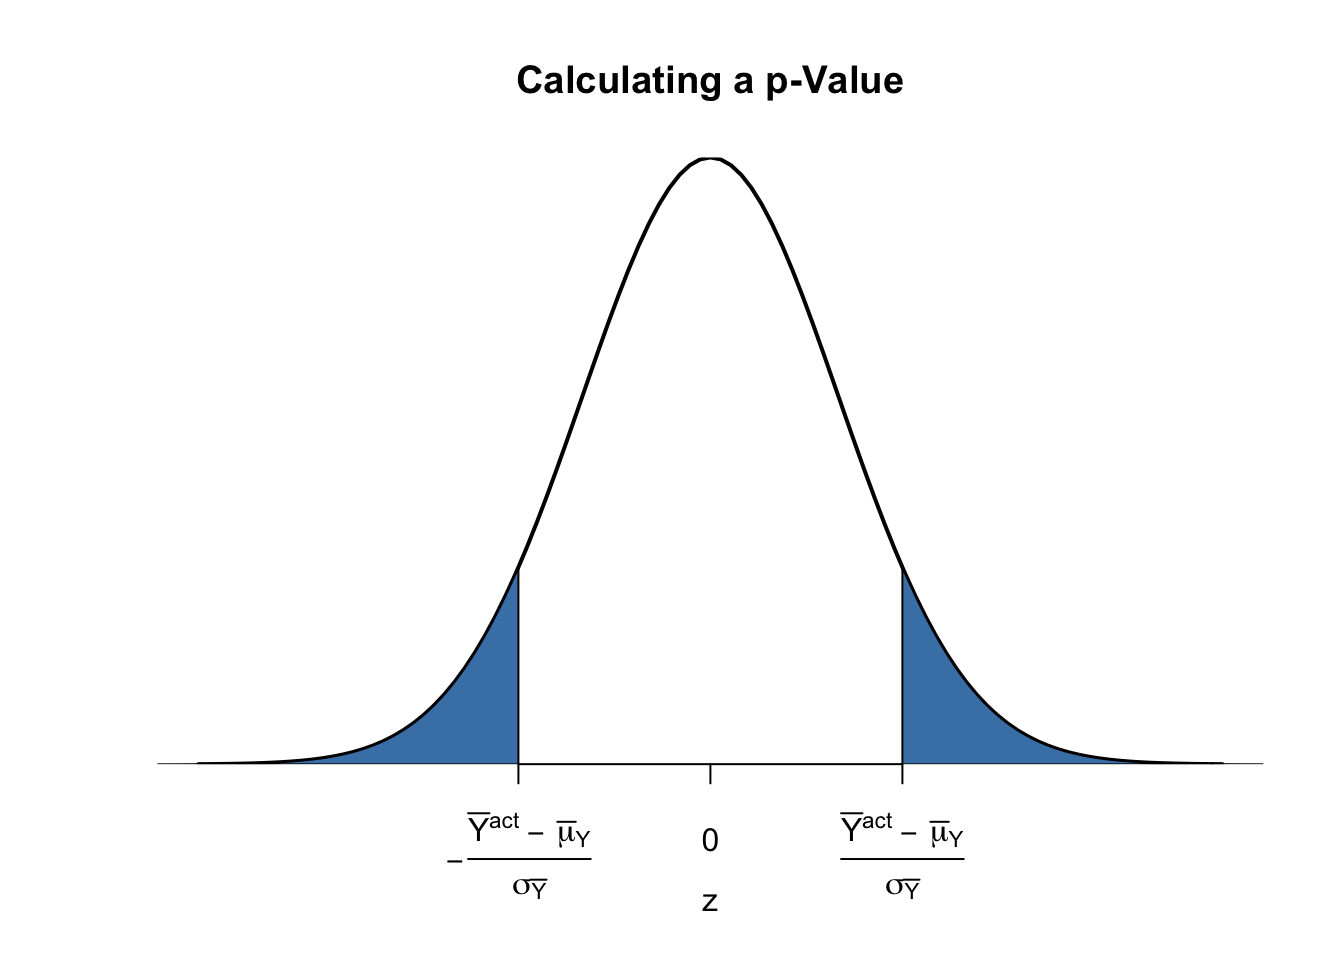
\includegraphics{URFITE_files/figure-latex/unnamed-chunk-71-1} \end{center}

\hypertarget{lrwor}{\chapter{Linear Regression with One
Regressor}\label{lrwor}}

This chapter introduces the basics in linear regression and shows how to
perform regression analysis in R. In linear regression, the aim is to
model the relationship between a dependent variable \(Y\) and one or
more explanatory variables denoted as \(X_1, X_2, \dots, X_k\).
Following the book we will focus on the concept of simple linear
regression throughout the whole chapter. In simple linear regression,
there is just one explanatory variable \(X_1\). If for example a school
cuts the class sizes by hiring new teachers, that is the school lowers
the student-teacher ratios of their classes, \(X_1\), how would this
affect the performance of the students involved in a standardized
test,\(Y\)? With linear regression we can not only examine whether the
student-teacher ratio \emph{does have} an impact on the test results but
we can also learn about the \emph{direction} and the \emph{strength} of
this effect.

To start with an easy example, consider the following combinations of
average test score and the average student-teacher ratio in some
fictional school disctrics.

1

2

3

4

5

6

7

TestScore

680

640

670

660

630

660.0

635

STR

15

17

19

20

22

23.5

25

To work with these data in R we begin by creating two vectors: one for
the student-teacher ratios (\texttt{STR}) and one for test scores
(\texttt{TestScore}), both containing the data from the table above.

\begin{Shaded}
\begin{Highlighting}[]
\CommentTok{# Create sample data}
\NormalTok{STR <-}\StringTok{ }\KeywordTok{c}\NormalTok{(}\DecValTok{15}\NormalTok{, }\DecValTok{17}\NormalTok{, }\DecValTok{19}\NormalTok{, }\DecValTok{20}\NormalTok{, }\DecValTok{22}\NormalTok{, }\FloatTok{23.5}\NormalTok{, }\DecValTok{25}\NormalTok{)}
\NormalTok{TestScore <-}\StringTok{ }\KeywordTok{c}\NormalTok{(}\DecValTok{680}\NormalTok{, }\DecValTok{640}\NormalTok{, }\DecValTok{670}\NormalTok{, }\DecValTok{660}\NormalTok{, }\DecValTok{630}\NormalTok{, }\DecValTok{660}\NormalTok{, }\DecValTok{635}\NormalTok{) }

\CommentTok{# Print out sample data}
\NormalTok{STR}
\end{Highlighting}
\end{Shaded}

\begin{verbatim}
## [1] 15.0 17.0 19.0 20.0 22.0 23.5 25.0
\end{verbatim}

\begin{Shaded}
\begin{Highlighting}[]
\NormalTok{TestScore}
\end{Highlighting}
\end{Shaded}

\begin{verbatim}
## [1] 680 640 670 660 630 660 635
\end{verbatim}

If we use a simple linear regression model, we assume that the true
relationship between both variables can be represented by a straight
line, formally

\[ Y = b \cdot X + a. \]

For now, let us suppose that the true function which relates test score
and student-teacher ratio to each other is

\[TestScore = 713 - 3 \times STR.\]

If possible, it is always a good idea to visualize the data You work
with in an appropriate way. For our purpose it is suitable to use the
function \texttt{plot()} to produce a scatterplot with \texttt{STR} on
the \(X\)-axis and \texttt{TestScore} on the \(Y\) axis. An easy way to
do so is to call
\texttt{plot(y\_variable\ \textasciitilde{}\ x\_variable)} whereby
\texttt{y\_variable} and \texttt{x\_variable} are placeholders for the
vectors of observations we want to plot. Furthermore, we might want to
add the true relationship to the plot. To draw a straight line, R
provides the function \texttt{abline()}. We just have to call this
function with arguments \texttt{a} (representing the intercept) and
\texttt{b} (representing the slope) after executing \texttt{plot()} in
order to add the line to our scatterplot.

The following code reproduces figure 4.1 from the textbook.

\begin{Shaded}
\begin{Highlighting}[]
\CommentTok{# create a scatter plot of the data}
\KeywordTok{plot}\NormalTok{(TestScore }\OperatorTok{~}\StringTok{ }\NormalTok{STR)}
\CommentTok{# add the true relationship to the plot}
\KeywordTok{abline}\NormalTok{(}\DataTypeTok{a =} \DecValTok{713}\NormalTok{, }\DataTypeTok{b =} \OperatorTok{-}\DecValTok{3}\NormalTok{)}
\end{Highlighting}
\end{Shaded}

\begin{center}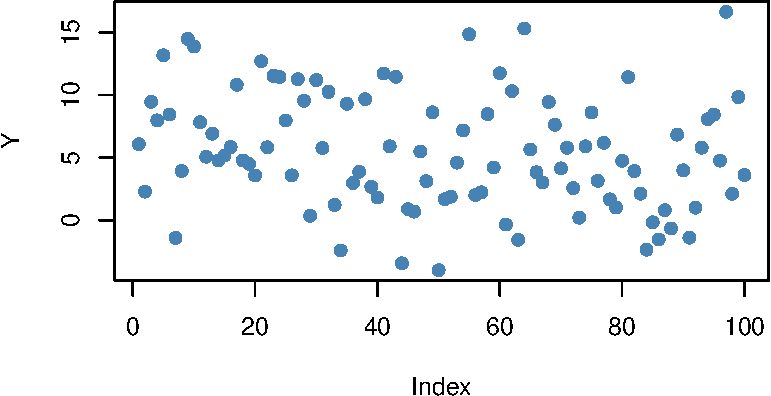
\includegraphics{URFITE_files/figure-latex/unnamed-chunk-73-1} \end{center}

We find that our line does not touch any of the points although we
claimed that it represents the true relationship. The reason for this is
the core problem of statistics, \emph{randomness}. Most of the time
there are influences which cannot be explained in a purely deterministic
fashion and thus exacerbate finding the true relationship.

In order to account for these differences between observed data and the
true relationship, we extend our model from above by an \emph{error
term} \(u\) which covers these random effects. Put differently, \(u\)
accounts for all the differences between the true regression line and
the actual observed data. Beside pure randomness, these deviations could
also arise from measerment errors or, as will be discussed later, could
be the consequence of leaving out other factors that are relevant in
explaining the dependent variable. Which other factor are plausible in
our example? For one thing, the test scores might be driven by the
teachers quality and the background of the students. It is also
imaginable that in some classes, the students were lucky on the test
days and thus achieved higher scores. For now, we will summarize such
influences by an additive component:

\[ TestScore = \beta_0 + \beta_1 \times STR + \text{other factors} \]

Of course this idea is very general as it can be easily extented to
other situations that can be described with a linear model. The basic
linear regression function we will work with hence is

\[ Y_i = \beta_0 + \beta_1 X_i + u_i. \]

Key Concept 4.1 summarizes the terminology of the simple linear
regression model.

Key Concept 4.1

Terminology for the Linear Regression Model with a Single Regressor

The linear regression model is

\[Y_i = \beta_0 + \beta_1 X_1 + u_i \]

where

\begin{itemize}
\tightlist
\item
  the subscript \(i\) runs over the observations, \(i = 1\), \ldots{},
  \(n\)
\item
  \(Y_i\) is the \emph{dependent variable}, the \emph{regressand}, or
  simply the \emph{left-hand variable}
\item
  \(X_i\) is the \emph{independent variable}, the \emph{regressor}, or
  simply the \emph{right-hand variable}
\item
  \(Y = \beta_0 + \beta_1 X\) is the \emph{population regression line}
  also called the \emph{population regression function}
\item
  \(\beta_0\) is the \emph{intercept} of the population regression line
\item
  \(\beta_1\) is the \emph{slope} of the population regression line
\item
  \(u_i\) is the \emph{error term}
\end{itemize}

\section{Estimating the Coefficients of the Linear Regression
Model}\label{estimating-the-coefficients-of-the-linear-regression-model}

In practice, the intercept \(\beta_0\) and slope \(\beta_1\)of the
population regression line are unknown. Therefore, we must employ data
to estimate both unknown parameters. In the following a real world
example will be used to demonstrate how this is achieved. We want to
relate test scores to student-teacher ratios measured in californian
schools. The test score is the district-wide average of reading and math
scores for fifth graders. Again, the class size is measured as the
number of students divided by the number of teachers (the
student-teacher ratio). As for the data, the California School dataset
(\texttt{CASchools}) comes with a R package called AER, an acronym for
\href{https://cran.r-project.org/web/packages/AER/AER.pdf}{Applied
Econometrics with R}. After installing the package with
\texttt{install.packages("AER")} and attaching it with
\texttt{library("AER")} the dataset can be loaded using the
\texttt{data} function.

\begin{Shaded}
\begin{Highlighting}[]
\CommentTok{# install the AER package (once)}
\KeywordTok{install.packages}\NormalTok{(}\StringTok{"AER"}\NormalTok{)}

\CommentTok{# load the AER package }
\KeywordTok{library}\NormalTok{(AER)   }

\CommentTok{# load the the data set in the workspace}
\KeywordTok{data}\NormalTok{(CASchools) }
\end{Highlighting}
\end{Shaded}

Note that once a package has been installed it is available for use at
further occasions when invoked with \texttt{library()} --- there is no
need to run \texttt{install.packages("...")} again!

For several reasons it is interesting to know what kind of object we are
dealing with. \texttt{class(object\_name)} returns the type (class) of
an object. Depending on the class of an object some functions (such as
\texttt{plot()} and \texttt{summary()}) behave differently.

Let us check the class of the object \texttt{CASchools}.

\begin{Shaded}
\begin{Highlighting}[]
\KeywordTok{class}\NormalTok{(CASchools)}
\end{Highlighting}
\end{Shaded}

\begin{verbatim}
## [1] "data.frame"
\end{verbatim}

It turns out that \texttt{CASchools} is of class \texttt{data.frame}
which is a convienient format to work with.

With help of the function \texttt{head()} we get a first overview of our
data. This function shows only the first 6 rows of the data set which
prevents an overcrowded console output.

\BeginKnitrBlock{rmdnote}
Press ctrl + L to clear the console. This command deletes any code that
has been typed in and executed by You or printed to the console by R
functions. Good news is: anything else is left untouched. You neither
loose defined variables and alike nor the code history. It is still
possible to recall previously executed R commands using the up and down
keys. If You are working in RStudio, press ctrl + Up on Your keyboard
(CMD + Up on a mac) to review a list of previously entered commands.
\EndKnitrBlock{rmdnote}

\begin{Shaded}
\begin{Highlighting}[]
\KeywordTok{head}\NormalTok{(CASchools)}
\end{Highlighting}
\end{Shaded}

\begin{verbatim}
##   district                          school  county grades students
## 1    75119              Sunol Glen Unified Alameda  KK-08      195
## 2    61499            Manzanita Elementary   Butte  KK-08      240
## 3    61549     Thermalito Union Elementary   Butte  KK-08     1550
## 4    61457 Golden Feather Union Elementary   Butte  KK-08      243
## 5    61523        Palermo Union Elementary   Butte  KK-08     1335
## 6    62042         Burrel Union Elementary  Fresno  KK-08      137
##   teachers calworks   lunch computer expenditure    income   english  read
## 1    10.90   0.5102  2.0408       67    6384.911 22.690001  0.000000 691.6
## 2    11.15  15.4167 47.9167      101    5099.381  9.824000  4.583333 660.5
## 3    82.90  55.0323 76.3226      169    5501.955  8.978000 30.000002 636.3
## 4    14.00  36.4754 77.0492       85    7101.831  8.978000  0.000000 651.9
## 5    71.50  33.1086 78.4270      171    5235.988  9.080333 13.857677 641.8
## 6     6.40  12.3188 86.9565       25    5580.147 10.415000 12.408759 605.7
##    math
## 1 690.0
## 2 661.9
## 3 650.9
## 4 643.5
## 5 639.9
## 6 605.4
\end{verbatim}

We find that the dataset consists of plenty of variables and most of
them are numeric.

By the way: an alternative to \texttt{class()} and \texttt{head()} is
\texttt{str()} which is deduced from `structure' and gives a
comprehensive overview of the object. Try this!

Turning back to \texttt{CASchools}, the two variables we are intersted
in (i.e.~average test score and the student-teacher ratio) are
\emph{not} included. However, it is possible to calculate both from the
provided data. To obtain the student-teacher ratios, we simply divide
the number of students by the number of teachers. The avarage test score
is the arithmetic mean of the test score for reading and the score of
the math test. The next code chunk shows how the two variables can be
constructed and how they are appended to \texttt{CASchools} which is a
data.frame.

\begin{Shaded}
\begin{Highlighting}[]
\CommentTok{# compute STR and append it to CASchools}
\NormalTok{CASchools}\OperatorTok{$}\NormalTok{STR <-}\StringTok{ }\NormalTok{CASchools}\OperatorTok{$}\NormalTok{students}\OperatorTok{/}\NormalTok{CASchools}\OperatorTok{$}\NormalTok{teachers }

\CommentTok{# compute TestScore and append it to CASchools}
\NormalTok{CASchools}\OperatorTok{$}\NormalTok{score <-}\StringTok{ }\NormalTok{(CASchools}\OperatorTok{$}\NormalTok{read }\OperatorTok{+}\StringTok{ }\NormalTok{CASchools}\OperatorTok{$}\NormalTok{math)}\OperatorTok{/}\DecValTok{2}     
\end{Highlighting}
\end{Shaded}

If we ran \texttt{head(CASchools)} again we would find the two variables
of interest as additional columns named \texttt{STR} and \texttt{score}
(check this!).

Table 4.1 from the text book summarizes the distribution of test scores
and student-teacher ratios. There are several functions which can be
used to produce similar results within R:

\begin{itemize}
\item
  \texttt{mean()} (computes the arithmetic mean of the provided numbers)
\item
  \texttt{sd()} (computes the sample standard deviation)
\item
  \texttt{quantile()} (returns a vector of the specified quantiles for
  the data)
\end{itemize}

The next code chunk shows how to achieve this. First, we compute summary
statistics on the coloumns \texttt{STR} and \texttt{score} of
\texttt{CASchools}. In order to have a nice display format we gather the
computed measures in a \texttt{data.frame} object named
\texttt{DistributionSummary}.

\begin{Shaded}
\begin{Highlighting}[]
\CommentTok{# compute sample averages of STR and score}
\NormalTok{avg_STR <-}\StringTok{ }\KeywordTok{mean}\NormalTok{(CASchools}\OperatorTok{$}\NormalTok{STR) }
\NormalTok{avg_score <-}\StringTok{ }\KeywordTok{mean}\NormalTok{(CASchools}\OperatorTok{$}\NormalTok{score)}

\CommentTok{# compute sample standard deviations of STR and score}
\NormalTok{sd_STR <-}\StringTok{ }\KeywordTok{sd}\NormalTok{(CASchools}\OperatorTok{$}\NormalTok{STR) }
\NormalTok{sd_score <-}\StringTok{ }\KeywordTok{sd}\NormalTok{(CASchools}\OperatorTok{$}\NormalTok{score)}

\CommentTok{# set up a vector of percentiles and compute the quantiles }
\NormalTok{quantiles <-}\StringTok{ }\KeywordTok{c}\NormalTok{(}\FloatTok{0.10}\NormalTok{, }\FloatTok{0.25}\NormalTok{, }\FloatTok{0.4}\NormalTok{, }\FloatTok{0.5}\NormalTok{, }\FloatTok{0.6}\NormalTok{, }\FloatTok{0.75}\NormalTok{, }\FloatTok{0.9}\NormalTok{)}
\NormalTok{quant_STR <-}\StringTok{ }\KeywordTok{quantile}\NormalTok{(CASchools}\OperatorTok{$}\NormalTok{STR, quantiles)}
\NormalTok{quant_score <-}\StringTok{ }\KeywordTok{quantile}\NormalTok{(CASchools}\OperatorTok{$}\NormalTok{score, quantiles)}

\CommentTok{# gather everything in a data.frame }
\NormalTok{DistributionSummary <-}\StringTok{ }\KeywordTok{data.frame}\NormalTok{(}
                                  \DataTypeTok{Average =} \KeywordTok{c}\NormalTok{(avg_STR, avg_score), }
                                  \DataTypeTok{StandardDeviation =} \KeywordTok{c}\NormalTok{(sd_STR, sd_score), }
                                  \DataTypeTok{quantile =} \KeywordTok{rbind}\NormalTok{(quant_STR, quant_score)}
\NormalTok{                                  )}

\CommentTok{# print the summary to the console}
\NormalTok{DistributionSummary}
\end{Highlighting}
\end{Shaded}

\begin{verbatim}
##               Average StandardDeviation quantile.10. quantile.25.
## quant_STR    19.64043          1.891812      17.3486     18.58236
## quant_score 654.15655         19.053347     630.3950    640.05000
##             quantile.40. quantile.50. quantile.60. quantile.75.
## quant_STR       19.26618     19.72321      20.0783     20.87181
## quant_score    649.06999    654.45000     659.4000    666.66249
##             quantile.90.
## quant_STR       21.86741
## quant_score    678.85999
\end{verbatim}

The standard distribution
(\href{https://stat.ethz.ch/R-manual/R-devel/library/base/html/00Index.html}{the
Base R package}) of R already contains a \texttt{summary} function which
can be applied to objects of class \texttt{data.frame}. Type and execute
\texttt{summary(STR)}!

As done for the sample data, we use \texttt{plot()} for a visual survey.
This allows us to detect specific characteristics of our data, such as
outliers which are hard to discover by looking at mere numbers. This
time we add some additional arguments to the \texttt{plot()} function.

The first argument in our call of \texttt{plot()},
\texttt{score\ \textasciitilde{}\ STR}, is again a formula that states
the dependent variable and the regressor. However, this time the two
variables are not saved in seperate vectors but are columns of
\texttt{CASchools}. Therefore, R would not find the variables without
the argument \texttt{data} beeing correctly specified. \texttt{data}
must be in accordance with the name of the \texttt{data.frame} to which
the variables belong, in this case \texttt{CASchools}. Further arguments
are used to change the appearance of the plot: while \texttt{main} adds
a title, \texttt{xlab} and \texttt{ylab} are adding custom labels to
both axes.

\begin{Shaded}
\begin{Highlighting}[]
\KeywordTok{plot}\NormalTok{(score }\OperatorTok{~}\StringTok{ }\NormalTok{STR, }
     \DataTypeTok{data =}\NormalTok{ CASchools,}
     \DataTypeTok{main =} \StringTok{"Scatterplot of TestScore and STR"}\NormalTok{, }
     \DataTypeTok{xlab =} \StringTok{"STR (X)"}\NormalTok{,}
     \DataTypeTok{ylab =} \StringTok{"Test Score (Y)"}
\NormalTok{)}
\end{Highlighting}
\end{Shaded}

\begin{center}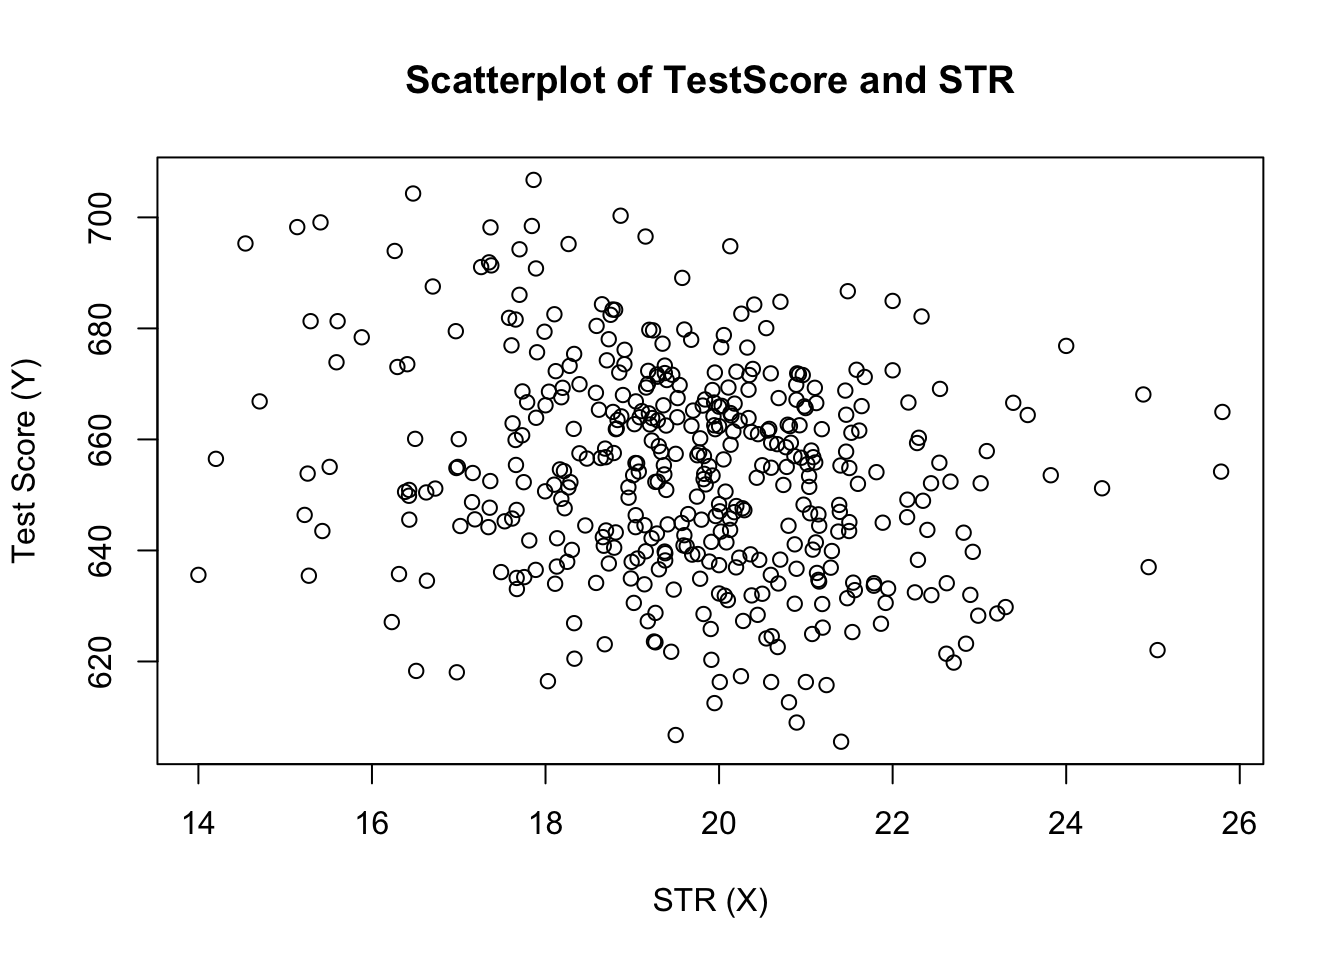
\includegraphics{URFITE_files/figure-latex/unnamed-chunk-79-1} \end{center}

The plot (figure 4.2 in the book) shows the scatterplot of all
observations on student-teacher ratio and Test score. We see that the
points are strongly scatterd and an apparent relationship cannot be
detected by only looking at them. Yet it can be assumed that both
variables are negatively correlated, that is we expect to observe lower
test scores in bigger classes.

The function \texttt{cor()} (type and execute \texttt{?cor} for further
info), can be used to compute the correlation between 2 \emph{numerical}
vectors.

\begin{Shaded}
\begin{Highlighting}[]
\KeywordTok{cor}\NormalTok{(CASchools}\OperatorTok{$}\NormalTok{STR, CASchools}\OperatorTok{$}\NormalTok{score)}
\end{Highlighting}
\end{Shaded}

\begin{verbatim}
## [1] -0.2263627
\end{verbatim}

As the scatterplot already suggests, the correlation is negative but
rather weak.

The task we are facing now is to find a line which fits best to the
data. Of course we could simply stick with graphical inspection and
correlation analysis and then select the best fitting line by
eyeballing. However, this is pretty unscientific and prone to subjective
perception: different students would draw different regression lines. On
this account, we are interested in techniques that are more
sophisticated. Such a technique is ordinary least squares (OLS)
estimation.

\subsection*{The Ordinary Least Squares
Estimator}\label{the-ordinary-least-squares-estimator}
\addcontentsline{toc}{subsection}{The Ordinary Least Squares Estimator}

The OLS estimator chooses the regression coefficients such that the
estimated regression line is as close as possible to the observed data
points. Thereby closeness is measured by the sum of the squared mistakes
made in predicting \(Y\) given \(X\). Let \(b_0\) and \(b_1\) be some
estimators of \(\beta_0\) and \(\beta_1\). Then the sum of squared
estimation mistakes can be expressed as

\[ \sum^n_{i = 1} (Y_i - b_0 - b_1 X_i)^2. \]

The OLS estimator in the simple regression model is the pair of
estimators for intercept and slope which minimizes the expression above.
The derivation of the OLS estimators for both parameters are presented
in Appendix 4.1 of the book. The results are summarized in Key Concept
4.2.

Key Concept 4.2

The OLS Estimator, Predicted Values, and Residuals

The OLS estimators of the slope \(\beta_1\) and the intercept
\(\beta_0\) in the simple linear regression model are

\begin{align}
  \hat\beta_1 & = \frac{ \sum_{i = 1}^n (X_i - \overline{X})(Y_i - \overline{Y}) } { \sum_{i=1}^n (X_i - \overline{X})^2}  \\
  \\
  \hat\beta_0 & =  \overline{Y} - \hat\beta_1 \overline{X} 
\end{align}

The OLS predicted values \(\widehat{Y}_i\) and residuals \(\hat{u}_i\)
are

\begin{align}
  \widehat{Y}_i & =  \hat\beta_0 + \hat\beta_1 X_i,\\
  \\
  \hat{u}_i & =  Y_i - \widehat{Y}_i. 
\end{align}

The estimated intercept \(\hat{\beta}_0\), the slope parameter
\(\hat{\beta}_1\), and the residuals \(\left(\hat{u}_i\right)\) are
computed from a sample of \(n\) observations of \(X_i\) and \(Y_i\),
\(i\), \(...\), \(n\). These are \emph{estimates} of the unkown true
population intercept \(\left(\beta_0 \right)\), slope
\(\left(\beta_1\right)\), and error term \((u_i)\).

We are aware that the results presented in Key Concept 4.2 are not very
intuitive at first glance. The following interactice application aims to
help You understand the mechanics of OLS. You can add observations by
clicking into the coordinate system where the data are represented by
points. If two or more observations are available, the application
computes a regression line using OLS and some statistics which are
displayed in the right panel. The results are updated as You add further
observations to the left panel. A double-click resets the application
i.e.~all data are removed.

There are many possible ways to compute \(\hat{\beta_0}\) and
\(\hat{\beta_1}\) in R. For example, we could implement the formulas
presented in Key Concept 4.2 with two of R's most basic functions:
\texttt{mean()} and \texttt{sum()}.

\begin{Shaded}
\begin{Highlighting}[]
\KeywordTok{attach}\NormalTok{(CASchools) }\CommentTok{#allows to use the variables contained in CASchools directly}
\end{Highlighting}
\end{Shaded}

\begin{verbatim}
## The following objects are masked from CASchools (pos = 10):
## 
##     calworks, computer, county, district, english, expenditure,
##     grades, income, lunch, math, read, school, score, STR,
##     students, teachers
\end{verbatim}

\begin{Shaded}
\begin{Highlighting}[]
\CommentTok{# compute beta_1 }
\NormalTok{beta_}\DecValTok{1}\NormalTok{ <-}\StringTok{ }\KeywordTok{sum}\NormalTok{((STR }\OperatorTok{-}\StringTok{ }\KeywordTok{mean}\NormalTok{(STR))}\OperatorTok{*}\NormalTok{(score }\OperatorTok{-}\StringTok{ }\KeywordTok{mean}\NormalTok{(score))) }\OperatorTok{/}\StringTok{ }\KeywordTok{sum}\NormalTok{((STR }\OperatorTok{-}\StringTok{ }\KeywordTok{mean}\NormalTok{(STR))}\OperatorTok{^}\DecValTok{2}\NormalTok{)}

\CommentTok{# compute beta_0}
\NormalTok{beta_}\DecValTok{0}\NormalTok{ <-}\StringTok{ }\KeywordTok{mean}\NormalTok{(score) }\OperatorTok{-}\StringTok{ }\NormalTok{beta_}\DecValTok{1} \OperatorTok{*}\StringTok{ }\KeywordTok{mean}\NormalTok{(STR)}

\CommentTok{# print the results to the console}
\NormalTok{beta_}\DecValTok{1}
\end{Highlighting}
\end{Shaded}

\begin{verbatim}
## [1] -2.279808
\end{verbatim}

\begin{Shaded}
\begin{Highlighting}[]
\NormalTok{beta_}\DecValTok{0}
\end{Highlighting}
\end{Shaded}

\begin{verbatim}
## [1] 698.9329
\end{verbatim}

Of course there are also other and even more manual ways to do the same
tasks. Luckily, OLS is one of the most widely-used estimation
techniques. Being a statistical programming language, R already contains
a built-in function named \texttt{lm()} (\textbf{l}inear \textbf{m}odel)
which can be used to carry out regression analysis.

The first argument of the function to be specified is, similar as in
\texttt{plot()}, the regression formula with the basic syntax
\texttt{y\ \textasciitilde{}\ x} where \texttt{y} is the dependent
variable and \texttt{x} the explanatory variable. The argument
\texttt{data} sets the data set to be used in the regression. We now
revisit the example from the book where the relationship between the
test scores and the class sizes is analysed. The following code uses
\texttt{lm()} to replicate the results presented in figure 4.3 in the
book.

\begin{Shaded}
\begin{Highlighting}[]
\CommentTok{# estimate the model and assign the result to linear_model}
\NormalTok{linear_model <-}\StringTok{ }\KeywordTok{lm}\NormalTok{(score }\OperatorTok{~}\StringTok{ }\NormalTok{STR, }\DataTypeTok{data =}\NormalTok{ CASchools)}

\CommentTok{# Print the standard output of the estimated lm object to the console }
\NormalTok{linear_model}
\end{Highlighting}
\end{Shaded}

\begin{verbatim}
## 
## Call:
## lm(formula = score ~ STR, data = CASchools)
## 
## Coefficients:
## (Intercept)          STR  
##      698.93        -2.28
\end{verbatim}

Let us add the estimated regression line to the plot. This time we also
enlarge ranges of both axes by setting the arguments \texttt{xlim} and
\texttt{ylim}.

\begin{Shaded}
\begin{Highlighting}[]
\CommentTok{# plot the data}
\KeywordTok{plot}\NormalTok{(score }\OperatorTok{~}\StringTok{ }\NormalTok{STR, }
     \DataTypeTok{data =}\NormalTok{ CASchools,}
     \DataTypeTok{main =} \StringTok{"Scatterplot of TestScore and STR"}\NormalTok{, }
     \DataTypeTok{xlab =} \StringTok{"STR (X)"}\NormalTok{,}
     \DataTypeTok{ylab =} \StringTok{"Test Score (Y)"}\NormalTok{,}
     \DataTypeTok{xlim =} \KeywordTok{c}\NormalTok{(}\DecValTok{10}\NormalTok{, }\DecValTok{30}\NormalTok{),}
     \DataTypeTok{ylim =} \KeywordTok{c}\NormalTok{(}\DecValTok{600}\NormalTok{, }\DecValTok{720}\NormalTok{)}
\NormalTok{     )}

\CommentTok{# add the regression line}
\KeywordTok{abline}\NormalTok{(linear_model) }
\end{Highlighting}
\end{Shaded}

\begin{center}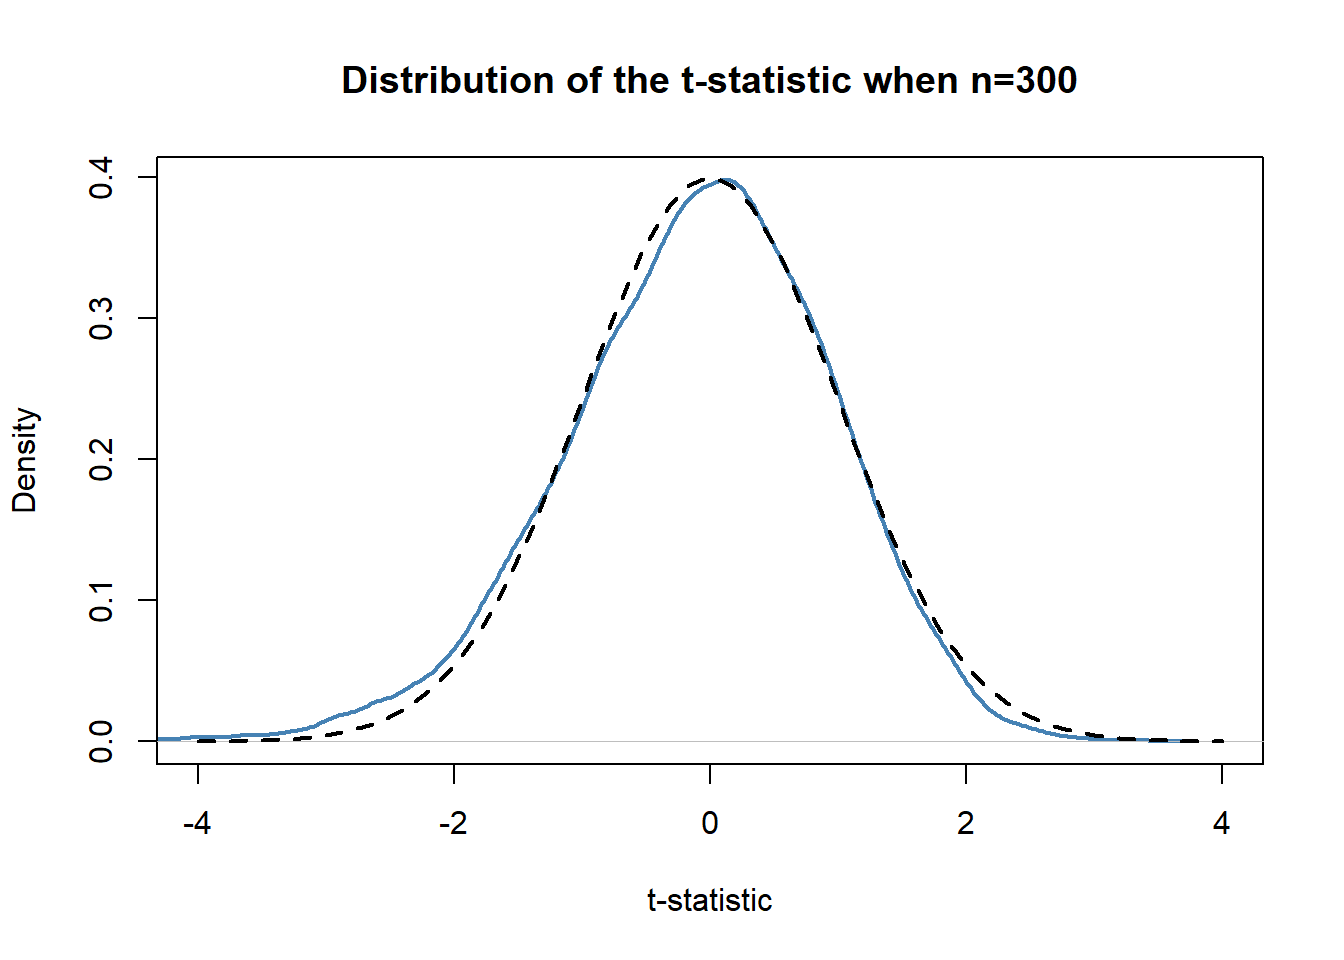
\includegraphics{URFITE_files/figure-latex/unnamed-chunk-83-1} \end{center}

Did you notice that this time, we did not pass the intercept and slope
parameters to \texttt{abline}? If you call \texttt{abline} on an object
of class \texttt{lm} that only contains a single regressor variable, R
draws the regression line automatically!

\section{Measures of Fit}\label{measures-of-fit}

After estimating a linear regression, the question occurs how well that
regression line describes the data. Are the observations tightly
clustered arround the regression line, or are they spread out? Both, the
\(R^2\) and the \emph{standard error of the regression} (\(SER\))
measure how well the OLS Regression line fits the data.

\subsection*{\texorpdfstring{The \(R^2\)}{The R\^{}2}}\label{the-r2}
\addcontentsline{toc}{subsection}{The \(R^2\)}

The \(R^2\) is the fraction of sample variance of \(Y_i\) that is
explained by \(X_i\). Mathemethically, the \(R^2\) can be written as the
ratio of the explained sum of squares to the total sum of squares. The
\emph{explained sum of squares} (\(ESS\)) is the sum of squared
deviations of the predicted values, \(\hat{Y_i}\), from the average of
the \(Y_i\). The \emph{total sum of squares} (\(TSS\)) is the sum of
squared deviations of the \(Y_i\) from their average.

\begin{align}
  ESS & =  \sum_{i = 1}^n \left( \hat{Y_i} - \overline{Y} \right)^2   \\
  \\
  TSS & =  \sum_{i = 1}^n \left( Y_i - \overline{Y} \right)^2   \\
  \\
  R^2 & = \frac{ESS}{TSS}
\end{align}

Since \(TSS = ESS + SSR\) we can also write

\[ R^2 = 1- \frac{SSR}{TSS} \]

where \(SSR\) is the sum of squared residuals, a measure for the errors
made when predicting the \(Y\) by \(X\). The \(SSR\) is defined as

\[ SSR = \sum_{i=1}^n \hat{u}_i^2. \]

\(R^2\) lies between \(0\) and \(1\). It is easy to see that a perfect
fit, i.e.~no errors made when fitting the regression line, implies
\(R^2 = 1\) since then we have \(SSR=0\). On the contrary, if our
estimated regression line does not explain any variation in the \(Y_i\),
we have \(ESS=0\) and consequently \(R^2=0\).

\subsection*{Standard Error of the
Regression}\label{standard-error-of-the-regression}
\addcontentsline{toc}{subsection}{Standard Error of the Regression}

The \emph{Standard Error of the Regression} (\(SER\)) is an estimator of
the standard deviation of the regression error \(\hat{u}_i\). As such it
measure the magnitude of a typical deviation from the regression,
i.e.~the magnitude of a typical regression error.

\[ SER = s_{\hat{u}} = \sqrt{s_{\hat{u}}^2} \ \ \ \text{where} \ \ \ s_{\hat{u} }^2 = \frac{1}{n-2} \sum_{i = 1}^n \hat{u}^2_i = \frac{SSR}{n - 2} \]

Remember that the \(u_i\) are \emph{unobserved}. That is why we use
their estimated counterparts, the residuals \(\hat{u}_i\) instead. See
chapter 4.3 of the book for a more detailed comment on the \(SER\).

\subsection*{Application to the Test Score
Data}\label{application-to-the-test-score-data}
\addcontentsline{toc}{subsection}{Application to the Test Score Data}

Both measures of fit can be obtained by using the function
\texttt{summary()} with the \texttt{lm} object provided as the only
argument. Whereas the function \texttt{lm()} only prints out the
estimated coefficients to the console, \texttt{summary} provides
additional predefined information such as the regression's \(R^2\) and
the \(SER\).

\begin{Shaded}
\begin{Highlighting}[]
\NormalTok{mod_summary <-}\StringTok{ }\KeywordTok{summary}\NormalTok{(linear_model)}
\NormalTok{mod_summary}
\end{Highlighting}
\end{Shaded}

\begin{verbatim}
## 
## Call:
## lm(formula = score ~ STR, data = CASchools)
## 
## Residuals:
##     Min      1Q  Median      3Q     Max 
## -47.727 -14.251   0.483  12.822  48.540 
## 
## Coefficients:
##             Estimate Std. Error t value Pr(>|t|)    
## (Intercept) 698.9329     9.4675  73.825  < 2e-16 ***
## STR          -2.2798     0.4798  -4.751 2.78e-06 ***
## ---
## Signif. codes:  0 '***' 0.001 '**' 0.01 '*' 0.05 '.' 0.1 ' ' 1
## 
## Residual standard error: 18.58 on 418 degrees of freedom
## Multiple R-squared:  0.05124,    Adjusted R-squared:  0.04897 
## F-statistic: 22.58 on 1 and 418 DF,  p-value: 2.783e-06
\end{verbatim}

The \(R^2\) in the output is called `Multiple R-squared' and has the
value \(0.051\). Hence, \(5.1 \%\) of the variance of the dependent
variable \(score\) is explained by the explanatory variable \(STR\).
That is the regression explains some of the variance but much of the
variation in test scores remains unexplained (cf.~figure 4.3 in the
book).

The \(SER\) is called `Residual standard error' and takes the value
\(18.58\). The unit of the \(SER\) is the same as the unit of the
dependent variable. In our context we can interpret the value as
follows: on average the deviation of the actual achieved test score and
the regression line is \(18.58\) points.

Now, let us check whether the \texttt{summary()} function uses the same
definitions for \(R^2\) and \(SER\) as we do by computing them manually.

\begin{Shaded}
\begin{Highlighting}[]
\CommentTok{# compute R^2 manually}
\NormalTok{SSR <-}\StringTok{ }\KeywordTok{sum}\NormalTok{(mod_summary}\OperatorTok{$}\NormalTok{residuals}\OperatorTok{^}\DecValTok{2}\NormalTok{)}
\NormalTok{TSS <-}\StringTok{ }\KeywordTok{sum}\NormalTok{((score }\OperatorTok{-}\StringTok{ }\KeywordTok{mean}\NormalTok{(score))}\OperatorTok{^}\DecValTok{2}\NormalTok{)}
\NormalTok{R2 <-}\StringTok{ }\DecValTok{1} \OperatorTok{-}\StringTok{ }\NormalTok{SSR}\OperatorTok{/}\NormalTok{TSS}

\CommentTok{# print the value to the console}
\NormalTok{R2}
\end{Highlighting}
\end{Shaded}

\begin{verbatim}
## [1] 0.05124009
\end{verbatim}

\begin{Shaded}
\begin{Highlighting}[]
\CommentTok{# compute SER manually}
\NormalTok{n <-}\StringTok{ }\KeywordTok{nrow}\NormalTok{(CASchools)}
\NormalTok{SER <-}\StringTok{ }\KeywordTok{sqrt}\NormalTok{(SSR }\OperatorTok{/}\StringTok{ }\NormalTok{(n}\OperatorTok{-}\DecValTok{2}\NormalTok{))}

\CommentTok{# print the value to the console}
\NormalTok{SER}
\end{Highlighting}
\end{Shaded}

\begin{verbatim}
## [1] 18.58097
\end{verbatim}

We find that the results coincide. Note that the values provided by
\texttt{summary()} are rounded to two decimal places. Can You Do this
using R?

\section{The Least Squares
Assumptions}\label{the-least-squares-assumptions}

OLS performs well under a quite broad variety of different
circumstances. However, there are some assumptions which are posed on
the data which need to be satisfied in order to achieve reliable
results.

Key Concept 4.3

The Least Squares Assumptions

\[Y_i = \beta_0 + \beta_1 X_i + u_i \text{, } i = 1, ...,n\] where

\begin{enumerate}
\def\labelenumi{\arabic{enumi}.}
\tightlist
\item
  The error term \(u_i\) has conditional mean zero given \(X_i\):
  \(E(u_i|X_i) = 0\)
\item
  \((X_i,Y_i), i = 1,...,n\) are independent and identically distributed
  (i.i.d.) draws from their joint distribution
\item
  Large outliers are unlikely: \(X_i\) and \(Y_i\) have nonzero finite
  fourth moments
\end{enumerate}

\subsection*{Assumption \#1: The Error Term has Conditional Mean of
Zero}\label{assumption-1-the-error-term-has-conditional-mean-of-zero}
\addcontentsline{toc}{subsection}{Assumption \#1: The Error Term has
Conditional Mean of Zero}

This means that no matter which value we choose for \(X\), the error
term \(u\) must not show any systematic pattern and must have a mean of
\(0\). Consider the case that \(E(u) = 0\) but for low and high values
of \(X\), the error term tends to be positive and for midrange values of
\(X\) the error tends to be negative. We can use R to construct such an
example. To do so we generate our own data using R's build in random
number generators.

We will use the following functions You should be familiar with:

\begin{itemize}
\tightlist
\item
  \texttt{runif()} (generates uniformly distributed random numbers)
\item
  \texttt{rnorm()} (generates nomally distributed random numbers)
\item
  \texttt{predict()} (does predictions based on the results of model
  fitting functions like \texttt{lm()})
\item
  \texttt{lines()} (adds line segments to an existing plot)
\end{itemize}

We start by creating a vector containing values that are randomly
scattered on the domain \([-5,5]\). For our example we decide to
generate uniformly distributed random numbers. This can be done with the
function \texttt{runif()}. We also need to simulate the error term. For
this we generate normally distributed random numbers with a mean equal
to \(0\) and a variance of \(1\) using \texttt{rnorm()}. The \(Y\)
values are obtained as a quadratic function of the \(X\) values and the
error. After generating the data we estimate both a simple regression
model and a quadratic model that also includes the regressor \(X^2\).
Finally, we plot the simulated data and add a the estimated regression
line of a simple regression model as well as the predictions made with a
quadratic model to compare the fit graphically.

\begin{Shaded}
\begin{Highlighting}[]
\CommentTok{# set a random seed to make the results reproducible}
\KeywordTok{set.seed}\NormalTok{(}\DecValTok{321}\NormalTok{)}

\CommentTok{# simulate the data }
\NormalTok{X <-}\StringTok{ }\KeywordTok{runif}\NormalTok{(}\DecValTok{50}\NormalTok{, }\DataTypeTok{min =} \OperatorTok{-}\DecValTok{5}\NormalTok{, }\DataTypeTok{max =} \DecValTok{5}\NormalTok{)}
\NormalTok{u <-}\StringTok{ }\KeywordTok{rnorm}\NormalTok{(}\DecValTok{50}\NormalTok{, }\DataTypeTok{sd =} \DecValTok{5}\NormalTok{)  }
\NormalTok{## the true relation  }
\NormalTok{Y <-}\StringTok{ }\NormalTok{X}\OperatorTok{^}\DecValTok{2} \OperatorTok{+}\StringTok{ }\DecValTok{2}\OperatorTok{*}\NormalTok{X }\OperatorTok{+}\StringTok{ }\NormalTok{u                }

\CommentTok{# estimate a simple regression model }
\NormalTok{mod_simple <-}\StringTok{ }\KeywordTok{lm}\NormalTok{(Y }\OperatorTok{~}\StringTok{ }\NormalTok{X)}

\CommentTok{# predict using a quadratic model }
\NormalTok{prediction <-}\StringTok{ }\KeywordTok{predict}\NormalTok{(}\KeywordTok{lm}\NormalTok{(Y }\OperatorTok{~}\StringTok{ }\NormalTok{X }\OperatorTok{+}\StringTok{  }\KeywordTok{I}\NormalTok{(X}\OperatorTok{^}\DecValTok{2}\NormalTok{)), }\KeywordTok{data.frame}\NormalTok{(}\DataTypeTok{X =} \KeywordTok{sort}\NormalTok{(X)))}

\CommentTok{# plot the results}
\KeywordTok{plot}\NormalTok{(Y }\OperatorTok{~}\StringTok{ }\NormalTok{X)}
\KeywordTok{abline}\NormalTok{(mod_simple, }\DataTypeTok{col =} \StringTok{"red"}\NormalTok{)}
\KeywordTok{lines}\NormalTok{(}\KeywordTok{sort}\NormalTok{(X), prediction)}
\end{Highlighting}
\end{Shaded}

\begin{center}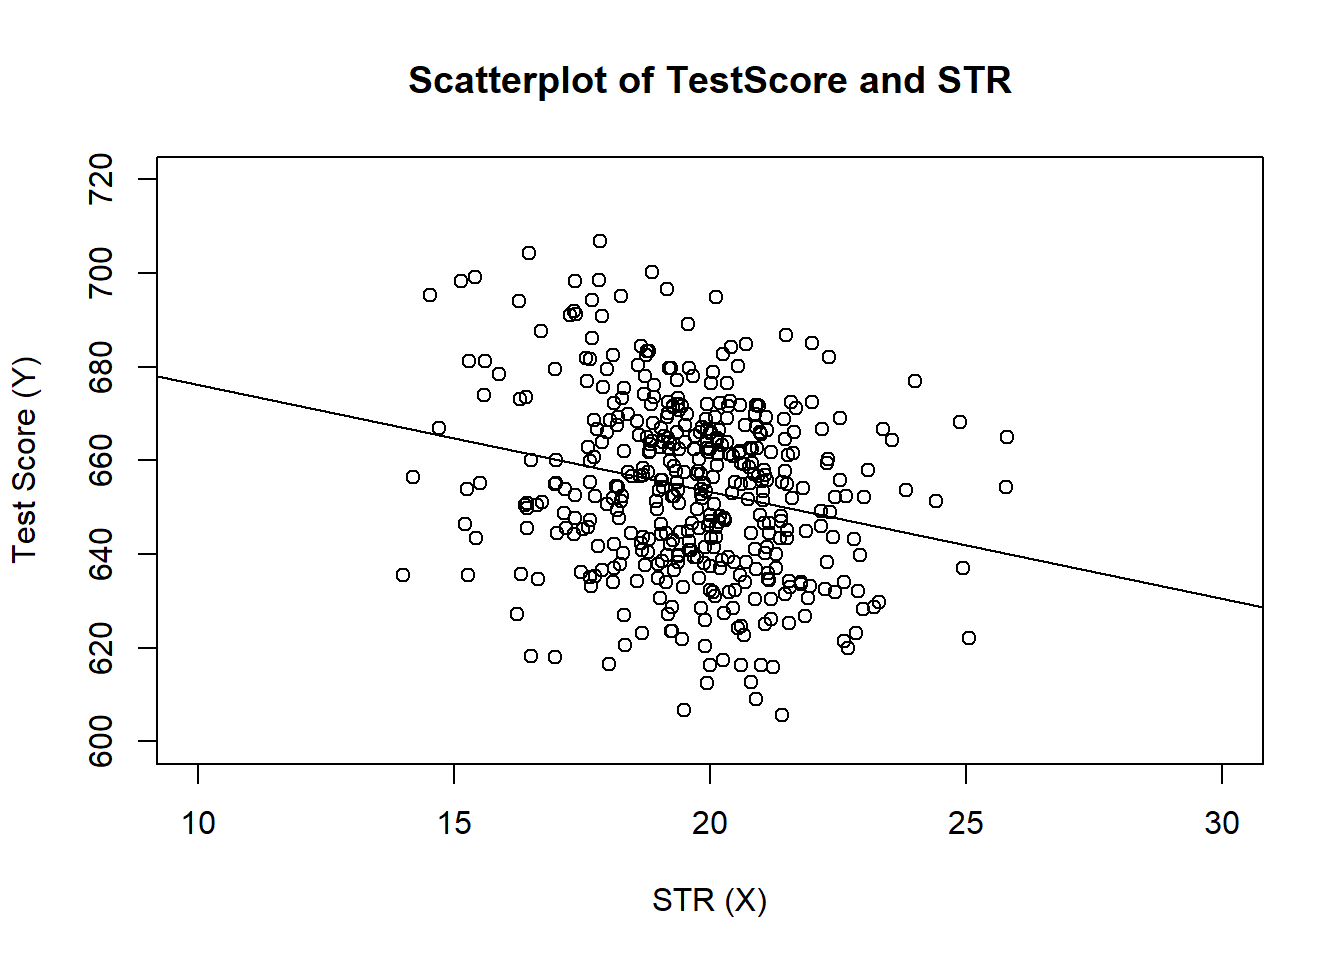
\includegraphics{URFITE_files/figure-latex/unnamed-chunk-86-1} \end{center}

This shows what is meant by \(E(u_i|X_i) = 0\):

Using the quadratic model (represented by the black curve) we see that
there are no systematic deviations of the observation from the predicted
relation. It is credible that the assumption is not violated when such a
model is employed. However, using a simple linear regression model we
see that the assumption is probably violated as \(E(u_i|X_i)\) varies
with the \(X_i\).

\subsection*{\texorpdfstring{Assumption \#2: All \((X_i, Y_i)\) are
Independently and Identically
Distributed}{Assumption \#2: All (X\_i, Y\_i) are Independently and Identically Distributed}}\label{assumption-2-all-x_i-y_i-are-independently-and-identically-distributed}
\addcontentsline{toc}{subsection}{Assumption \#2: All \((X_i, Y_i)\) are
Independently and Identically Distributed}

Most common sampling schemes used when collecting data from populations
produce i.i.d. samples. For example, we could use R's random number
generator to randomly select student IDs from a university's enrollment
list and record age \(X\) and earnings \(Y\) of the corresponding
students. This is a typical example of simple random sampling and
ensures that all the \((X_i,Y_i)\) are drawn randomly from the same
population.

A prominent example where the i.i.d. assumption is not fulfilled is time
series data where we have observations on the same unit over time. For
example, take \(X\) as the number of workers employed by a production
company over the course of time. Due to technological change, the
company makes job cuts periodically but there are also some
non-deterministic influences that relate to economics, politics and
alike. Using R we can simulate such a process and plot it.

We start the series with a total of 5000 workers and simulate the
reduction of employment with a simple autoregressive process that
exhibits a downward trend and has normal distributed errors:\footnote{See
  chapter 14 in the book for more on autoregressive processes and time
  series analysis in general.}

\[ employment_t = 0.98 \cdot employment_{t-1} + u_t \]

\begin{Shaded}
\begin{Highlighting}[]
\CommentTok{# set random seed}
\KeywordTok{set.seed}\NormalTok{(}\DecValTok{7}\NormalTok{)}

\CommentTok{# initialize the employment vector}
\NormalTok{X <-}\StringTok{ }\KeywordTok{c}\NormalTok{(}\DecValTok{5000}\NormalTok{,}\KeywordTok{rep}\NormalTok{(}\OtherTok{NA}\NormalTok{,}\DecValTok{99}\NormalTok{))}

\CommentTok{# generate a date vector}
\NormalTok{Date <-}\StringTok{ }\KeywordTok{seq}\NormalTok{(}\KeywordTok{as.Date}\NormalTok{(}\StringTok{"1951/1/1"}\NormalTok{), }\KeywordTok{as.Date}\NormalTok{(}\StringTok{"2050/1/1"}\NormalTok{), }\StringTok{"years"}\NormalTok{)}

\CommentTok{# generate time series observations with random influences}
\ControlFlowTok{for}\NormalTok{ (i }\ControlFlowTok{in} \DecValTok{2}\OperatorTok{:}\DecValTok{100}\NormalTok{) X[i] <-}\StringTok{ }\FloatTok{0.98}\OperatorTok{*}\NormalTok{X[i}\OperatorTok{-}\DecValTok{1}\NormalTok{] }\OperatorTok{+}\StringTok{ }\KeywordTok{rnorm}\NormalTok{(}\DecValTok{1}\NormalTok{, }\DataTypeTok{sd=}\DecValTok{200}\NormalTok{)}

\CommentTok{#plot the results}
\KeywordTok{plot}\NormalTok{(Date, X, }\DataTypeTok{type =} \StringTok{"l"}\NormalTok{, }\DataTypeTok{col=}\StringTok{"steelblue"}\NormalTok{, }\DataTypeTok{ylab =} \StringTok{"Workers"}\NormalTok{, }\DataTypeTok{xlab=}\StringTok{"Time (t)"}\NormalTok{)}
\end{Highlighting}
\end{Shaded}

\begin{center}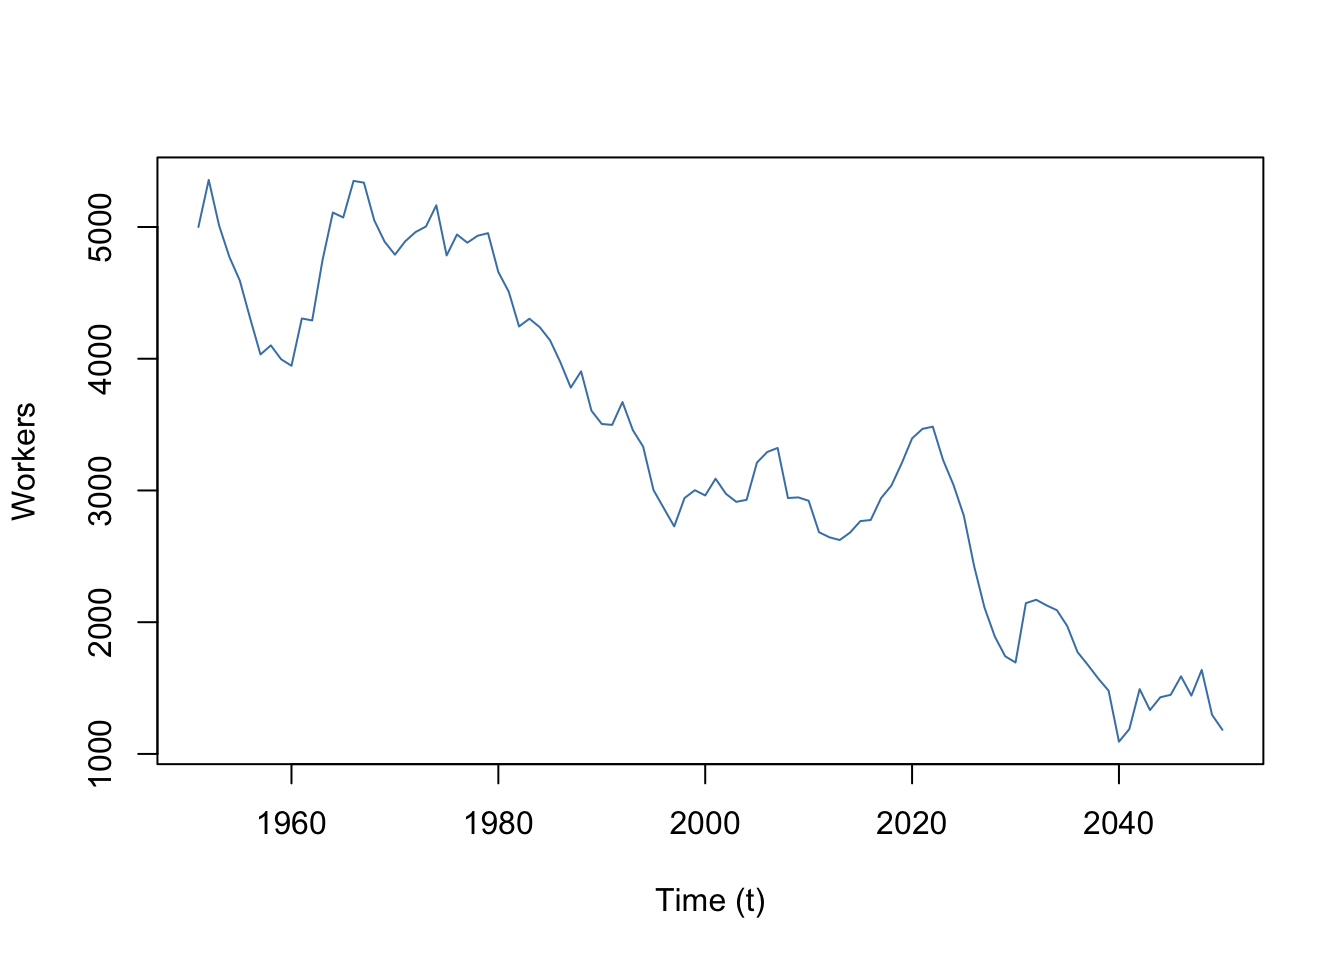
\includegraphics{URFITE_files/figure-latex/unnamed-chunk-87-1} \end{center}

It is evident that the observations on \(X\) cannot be independnet in
this example: the level of today's employment is correlated with
tomorrows employment level. Thus, the i.i.d. assumption is violated for
\(X\).

\subsection*{Assumption \#3: Large outliers are
unlikely}\label{assumption-3-large-outliers-are-unlikely}
\addcontentsline{toc}{subsection}{Assumption \#3: Large outliers are
unlikely}

It is easy to come up with situations where extreme observations,
i.e.~observations that deviate considerably from the usual range of the
data, may occur. Such observations are called outliers. Technically
speaking, assumption \#3 requires that \(X\) and \(Y\) have a finite
kurtosis.\footnote{See chapter 4.4 in the book.}

Common cases where we want to exclude or (if possible) correct such
outliers is when they are apperently typos, conversion errors or
measurement errors. Even if it seems that extreme observations have been
recorded correctly, it is advisable to exclude them before estimating a
model since OLS suffers from \emph{sensitivity to outliers}.

What does this mean? One can show that extreme observation receive heavy
weighting in the computation done with OLS. Therefore, outliers can lead
to strongly distorted estimates of regression coefficient. To get a
better impression of this, consider the following application where we
have placed some sample data on \(X\) and \(Y\) which are highly
correlated. The relation between \(X\) and \(Y\) seems to be explained
pretty good by the plotted regression line: all of the blue dots lie
close to the red line and we have \(R^2=0.92\).

Now go ahead and add a further observation at, say, \((18,2)\). This
clearly is an outlier. The result is quite striking: the estimated
regression line differs greatly from the one we adjudged to fit the data
well. The slope is heavily downward biased and \(R^2\) decreased to a
mere \(29\%\)! Double-click inside the coordinate system to reset the
app. Feel free to experiment. Choose different coordinates for the
outlier or add additional ones.

The following code roughly reproduces what is shown in figure 4.5 in the
book. As done above we use sample data generated using R's random number
functions \texttt{rnorm()} and \texttt{runif()}. We estimate simple
regression models based on the original data set and a modified set
where one observation is change to be an outlier and plot the results.
In order to understand the complete code You should be familiar with the
function \texttt{sort()} which sorts the entries of a numeric vector in
ascending order.

\begin{Shaded}
\begin{Highlighting}[]
\CommentTok{# set random seed}
\KeywordTok{set.seed}\NormalTok{(}\DecValTok{123}\NormalTok{)}

\CommentTok{# generate the data}
\NormalTok{X <-}\StringTok{ }\KeywordTok{sort}\NormalTok{(}\KeywordTok{runif}\NormalTok{(}\DecValTok{10}\NormalTok{, }\DataTypeTok{min =} \DecValTok{30}\NormalTok{, }\DataTypeTok{max =} \DecValTok{70}\NormalTok{ ))}
\NormalTok{Y <-}\StringTok{ }\KeywordTok{rnorm}\NormalTok{(}\DecValTok{10}\NormalTok{ , }\DataTypeTok{mean =} \DecValTok{200}\NormalTok{, }\DataTypeTok{sd =} \DecValTok{50}\NormalTok{)}
\NormalTok{Y[}\DecValTok{9}\NormalTok{] <-}\StringTok{ }\DecValTok{2000}

\CommentTok{# fit model with outlier}
\NormalTok{fit <-}\StringTok{ }\KeywordTok{lm}\NormalTok{(Y }\OperatorTok{~}\StringTok{ }\NormalTok{X)}

\CommentTok{# fit model without outlier}
\NormalTok{fitWithoutOutlier <-}\StringTok{ }\KeywordTok{lm}\NormalTok{(Y[}\OperatorTok{-}\DecValTok{9}\NormalTok{] }\OperatorTok{~}\StringTok{ }\NormalTok{X[}\OperatorTok{-}\DecValTok{9}\NormalTok{])}

\CommentTok{# plot the results}
\KeywordTok{plot}\NormalTok{(Y }\OperatorTok{~}\StringTok{ }\NormalTok{X)}
\KeywordTok{abline}\NormalTok{(fit)}
\KeywordTok{abline}\NormalTok{(fitWithoutOutlier, }\DataTypeTok{col =} \StringTok{"red"}\NormalTok{)}
\end{Highlighting}
\end{Shaded}

\begin{center}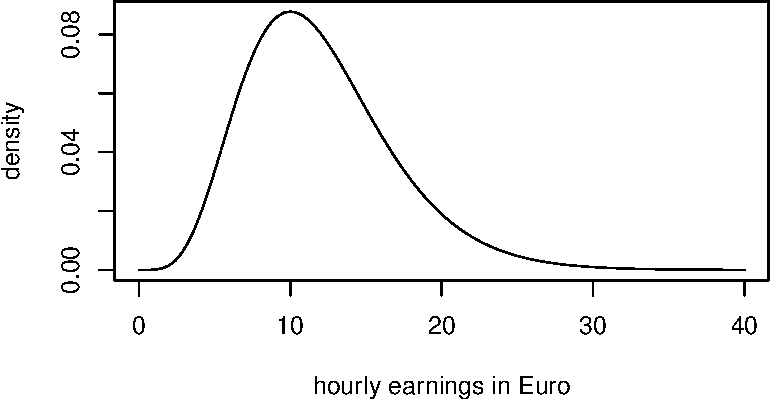
\includegraphics{URFITE_files/figure-latex/unnamed-chunk-88-1} \end{center}

\hypertarget{tsdotoe}{\section{The Sampling Distribution of the OLS
Estimator}\label{tsdotoe}}

Because the OLS estimators \(\hat{\beta_0}\) and \(\hat{\beta_1}\) are
computed from a randomly drawn sample, the estimators themselves are
random variables with a probability distribution --- the so-called
sampling distribution of the estimators --- which describes the values
they could take over different random samples. Although the sampling
distribution of \(\hat{\beta_0}\) and \(\hat{\beta_1}\) can be
complicated when the sample size is small and generally differs with the
number of observation, \(n\), it is possible to make certain statements
about it that hold for all \(n\). In particular
\[ E(\hat{\beta_0}) = \beta_0 \ \ \text{and} \ \  E(\hat{\beta_1}) = \beta_1,\]
that is, \(\hat\beta_0\) and \(\hat\beta_1\) are unbiased estimators of
\(\beta_0\) and \(\beta_1\), the true parameters. If the sample is
sufficiently large, by the central limit theorem the \emph{joint}
sampling distribution of the estimators is well approximated by the
bivariate normal distribution (2.1). This implies that the marginal
distributions are also normal in large samples. Core facts on the
large-sample distribution of \(\beta_0\) and \(\beta_1\) are presented
in Key Concept 4.4.

Key Concept 4.4

Large Sample Distribution of \(\hat\beta_0\) and \(\hat\beta_1\)

If the least squares assumptions in Key Concept 4.3 hold, then in large
samples \(\hat\beta_0\) and \(\hat\beta_1\) have a jointly normal
sampling distribution. The large sample normal distribution of
\(\hat\beta_1\) is \(N(\beta_1, \sigma^2_{\hat\beta_1})\), where the
variance of the distribution, \(\sigma^2_{\hat\beta_1}\), is

\[ \sigma^2_{\hat\beta_1} = \frac{1}{n} \frac{Var \left[ \left(X_i - \mu_X \right) u_i  \right]}  {\left[  Var \left(X_i \right)  \right]^2} \tag{4.1}. \]

The large sample normal distribution of \(\hat\beta_0\) is
\(N(\beta_0, \sigma^2_{\hat\beta_0})\), where

\[ \sigma^2_{\hat\beta_0} =  \frac{1}{n} \frac{Var \left( H_i u_i \right)}{ \left[  E \left(H_i^2  \right)  \right]^2 } \ , \ \text{where} \ \ H_i = 1 - \left[ \frac{\mu_X} {E \left( X_i^2\right)} \right] X_i. \tag{4.2} \]

\subsection*{R Simulation Study 1}\label{r-simulation-study-1}
\addcontentsline{toc}{subsection}{R Simulation Study 1}

Whether Key Koncept 4.4 really holds can be verified using R. First we
build our own population of \(100000\) observations in total. To do this
we need values for our independent variable \(X\), for the error term
\(u\), and the regression parameters \(\beta_0\) and \(\beta_1\). With
all this combined in a simple regression model, we can compute our
dependent variable \(Y\). In our example we generate the numbers
\(X_i\), \(i = 1\), \ldots{} ,\(100000\) by drawing a random sample from
a uniform distribution on the interval \([0,20]\). The realisations of
the error terms \(u_i\) are drawn from a standard normal distribution
with parameters \(\mu = 0\) and \(\sigma^2 = 100\) (note that
\texttt{rnorm()} requires \(\sigma\) as input for the argument
\texttt{sd}, see \texttt{?rnorm}). Furthermore we chose \(\beta_0 = -2\)
and \(\beta_1 = 3.5\) so the true model is

\[ Y_i = -2 + 3.5 \cdot X_i. \]

Finally, we store the results in a data.frame.

\begin{Shaded}
\begin{Highlighting}[]
\CommentTok{# simulate data}
\NormalTok{N <-}\StringTok{ }\DecValTok{100000}
\NormalTok{X <-}\StringTok{ }\KeywordTok{runif}\NormalTok{(N, }\DataTypeTok{min =} \DecValTok{0}\NormalTok{, }\DataTypeTok{max =} \DecValTok{20}\NormalTok{)}
\NormalTok{u <-}\StringTok{ }\KeywordTok{rnorm}\NormalTok{(N, }\DataTypeTok{sd =} \DecValTok{10}\NormalTok{)}

\CommentTok{# population regression}
\NormalTok{Y <-}\StringTok{ }\OperatorTok{-}\DecValTok{2} \OperatorTok{+}\StringTok{ }\FloatTok{3.5} \OperatorTok{*}\StringTok{ }\NormalTok{X }\OperatorTok{+}\StringTok{ }\NormalTok{u}
\NormalTok{population <-}\StringTok{ }\KeywordTok{data.frame}\NormalTok{(X, Y)}
\end{Highlighting}
\end{Shaded}

From now on we will consider the previously generated data as the true
population (which of course would be \emph{unknown} in a real world
application, otherwise there would not be a reason to do draw a random
sample in the first place). The knowledge about the true population and
the true relationship between \(Y\) and \(X\) can be used to verify the
statements made in Key Concept 4.4.

First, let us calculate the true variances \(\sigma^2_{\hat{\beta_0}}\)
and \(\sigma^2_{\hat{\beta_1}}\) for a randomly drawn sample of size
\(n = 100\).

\begin{Shaded}
\begin{Highlighting}[]
\CommentTok{# set sample size}
\NormalTok{n <-}\StringTok{ }\DecValTok{100}

\CommentTok{# compute the variance of hat_beta_0}
\NormalTok{H_i <-}\StringTok{ }\DecValTok{1} \OperatorTok{-}\StringTok{ }\KeywordTok{mean}\NormalTok{(X) }\OperatorTok{/}\StringTok{ }\KeywordTok{mean}\NormalTok{(X}\OperatorTok{^}\DecValTok{2}\NormalTok{) }\OperatorTok{*}\StringTok{ }\NormalTok{X}
\NormalTok{var_b0 <-}\StringTok{ }\KeywordTok{var}\NormalTok{(H_i }\OperatorTok{*}\StringTok{ }\NormalTok{u) }\OperatorTok{/}\StringTok{ }\NormalTok{(n }\OperatorTok{*}\StringTok{ }\KeywordTok{mean}\NormalTok{(H_i}\OperatorTok{^}\DecValTok{2}\NormalTok{)}\OperatorTok{^}\DecValTok{2}\NormalTok{ )}

\CommentTok{# compute the variance of hat_beta_1}
\NormalTok{var_b1 <-}\StringTok{ }\KeywordTok{var}\NormalTok{( ( X }\OperatorTok{-}\StringTok{ }\KeywordTok{mean}\NormalTok{(X) ) }\OperatorTok{*}\StringTok{ }\NormalTok{u ) }\OperatorTok{/}\StringTok{ }\NormalTok{(}\DecValTok{100} \OperatorTok{*}\StringTok{ }\KeywordTok{var}\NormalTok{(X)}\OperatorTok{^}\DecValTok{2}\NormalTok{)}
\end{Highlighting}
\end{Shaded}

\begin{Shaded}
\begin{Highlighting}[]
\CommentTok{# print variances to the console}
\NormalTok{var_b0}
\end{Highlighting}
\end{Shaded}

\begin{verbatim}
## [1] 4.045066
\end{verbatim}

\begin{Shaded}
\begin{Highlighting}[]
\NormalTok{var_b1}
\end{Highlighting}
\end{Shaded}

\begin{verbatim}
## [1] 0.03018694
\end{verbatim}

Now let us assume that we do not know the true values of \(\beta_0\) and
\(\beta_1\) and that it is not possible to observe the whole population.
However, we can observe a random sample of \(n\) observations. Then, it
would not be possible to compute the true parameters but we could obtain
estimates of \(\beta_0\) and \(\beta_1\) from the sample data using OLS.
However, we know that these estimates are outcomes of random variables
themselves since the observations are randomly sampled from the
population. Key Concept 4.4. describes their distributions for large
\(n\). When drawing a single sample of size \(n\) it is not possible to
make any statement about these distributions. Things change if we repeat
the sampling scheme many times and compute the estimates for each
sample: using such a procedure we simulate outcomes of the respective
distributions.

To achieve this in R, we employ the following approach:

\begin{itemize}
\tightlist
\item
  We assign the number of repetitions, say \(10000\), to \texttt{reps}.
  Then we initialize a matrix \texttt{fit} were the estimates obtained
  in each sampling iteration shall be stored row-wise. Thus \texttt{fit}
  has to be an array of dimensions \texttt{reps}\(\times2\).
\item
  In the next step we draw \texttt{reps} random sample of size
  \texttt{n} from the population and obtain the OLS estimates for each
  sample. The results are stored as row entries in the outcome matrix
  \texttt{fit}. This is done using a \texttt{for()} loop.
\item
  At last, we estimate variances of both coefficient estimators using
  the sampled outcomes and plot histograms of the latter. We also add
  plot of the density functions belonging to the distributions that
  follow from Key Concept 4.4. The function \texttt{bquote()} is used to
  obtain math expressions in the titels and labels of both plots. See
  \texttt{?bquote}.
\end{itemize}

\begin{Shaded}
\begin{Highlighting}[]
\CommentTok{# set repetitions and sample size}
\NormalTok{n <-}\StringTok{ }\DecValTok{100}
\NormalTok{reps <-}\StringTok{ }\DecValTok{10000}

\CommentTok{# initialize the matrix of outcomes}
\NormalTok{fit <-}\StringTok{ }\KeywordTok{matrix}\NormalTok{(}\DataTypeTok{ncol =} \DecValTok{2}\NormalTok{, }\DataTypeTok{nrow =}\NormalTok{ reps)}

\CommentTok{# loop sampling and estimating of the coefficients}
\ControlFlowTok{for}\NormalTok{ (i }\ControlFlowTok{in} \DecValTok{1}\OperatorTok{:}\NormalTok{reps)\{}
\NormalTok{ sample <-}\StringTok{ }\NormalTok{population[}\KeywordTok{sample}\NormalTok{(}\DecValTok{1}\OperatorTok{:}\NormalTok{N, n),]}
\NormalTok{ fit[i, ] <-}\StringTok{ }\KeywordTok{lm}\NormalTok{(Y }\OperatorTok{~}\StringTok{ }\NormalTok{X, }\DataTypeTok{data =}\NormalTok{ sample)}\OperatorTok{$}\NormalTok{coefficients}
\NormalTok{\}}

\CommentTok{# compute variance estimates using outcomes}
\KeywordTok{var}\NormalTok{(fit[ ,}\DecValTok{1}\NormalTok{])}
\end{Highlighting}
\end{Shaded}

\begin{verbatim}
## [1] 4.057089
\end{verbatim}

\begin{Shaded}
\begin{Highlighting}[]
\KeywordTok{var}\NormalTok{(fit[ ,}\DecValTok{2}\NormalTok{])}
\end{Highlighting}
\end{Shaded}

\begin{verbatim}
## [1] 0.03021784
\end{verbatim}

\begin{Shaded}
\begin{Highlighting}[]
\CommentTok{# plot histograms of beta_0 estimates}
\KeywordTok{hist}\NormalTok{(fit[ ,}\DecValTok{1}\NormalTok{], }
     \DataTypeTok{main =} \KeywordTok{bquote}\NormalTok{(The }\OperatorTok{~}\StringTok{ }\NormalTok{Distribution  }\OperatorTok{~}\StringTok{ }\NormalTok{of }\OperatorTok{~}\StringTok{ }\DecValTok{10000} \OperatorTok{~}\StringTok{ }\NormalTok{beta[}\DecValTok{0}\NormalTok{] }\OperatorTok{~}\StringTok{ }\NormalTok{Estimates), }
     \DataTypeTok{xlab =} \KeywordTok{bquote}\NormalTok{(}\KeywordTok{hat}\NormalTok{(beta)[}\DecValTok{0}\NormalTok{]), }
     \DataTypeTok{freq =}\NormalTok{ F)}
\CommentTok{# add true distribution to plot}
\KeywordTok{curve}\NormalTok{(}\KeywordTok{dnorm}\NormalTok{(x,}\OperatorTok{-}\DecValTok{2}\NormalTok{,}\KeywordTok{sqrt}\NormalTok{(var_b0)), }\DataTypeTok{add =}\NormalTok{ T, }\DataTypeTok{col=}\StringTok{"darkred"}\NormalTok{)}
\end{Highlighting}
\end{Shaded}

\begin{center}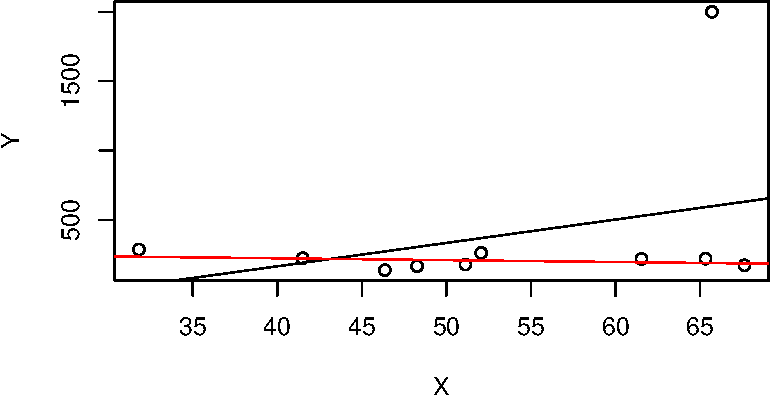
\includegraphics{URFITE_files/figure-latex/unnamed-chunk-92-1} \end{center}

\begin{Shaded}
\begin{Highlighting}[]
\CommentTok{# plot histograms of beta_1 estimates}
\KeywordTok{hist}\NormalTok{(fit[ ,}\DecValTok{2}\NormalTok{], }
     \DataTypeTok{main =} \KeywordTok{bquote}\NormalTok{(The }\OperatorTok{~}\StringTok{ }\NormalTok{Distribution  }\OperatorTok{~}\StringTok{ }\NormalTok{of }\OperatorTok{~}\StringTok{ }\DecValTok{10000} \OperatorTok{~}\StringTok{ }\NormalTok{beta[}\DecValTok{1}\NormalTok{] }\OperatorTok{~}\StringTok{ }\NormalTok{Estimates), }
     \DataTypeTok{xlab =} \KeywordTok{bquote}\NormalTok{(}\KeywordTok{hat}\NormalTok{(beta)[}\DecValTok{1}\NormalTok{]), }
     \DataTypeTok{freq =}\NormalTok{ F)}

\CommentTok{# add true distribution to plot}
\KeywordTok{curve}\NormalTok{(}\KeywordTok{dnorm}\NormalTok{(x,}\FloatTok{3.5}\NormalTok{,}\KeywordTok{sqrt}\NormalTok{(var_b1)), }\DataTypeTok{add =}\NormalTok{ T, }\DataTypeTok{col=}\StringTok{"darkred"}\NormalTok{)}
\end{Highlighting}
\end{Shaded}

\begin{center}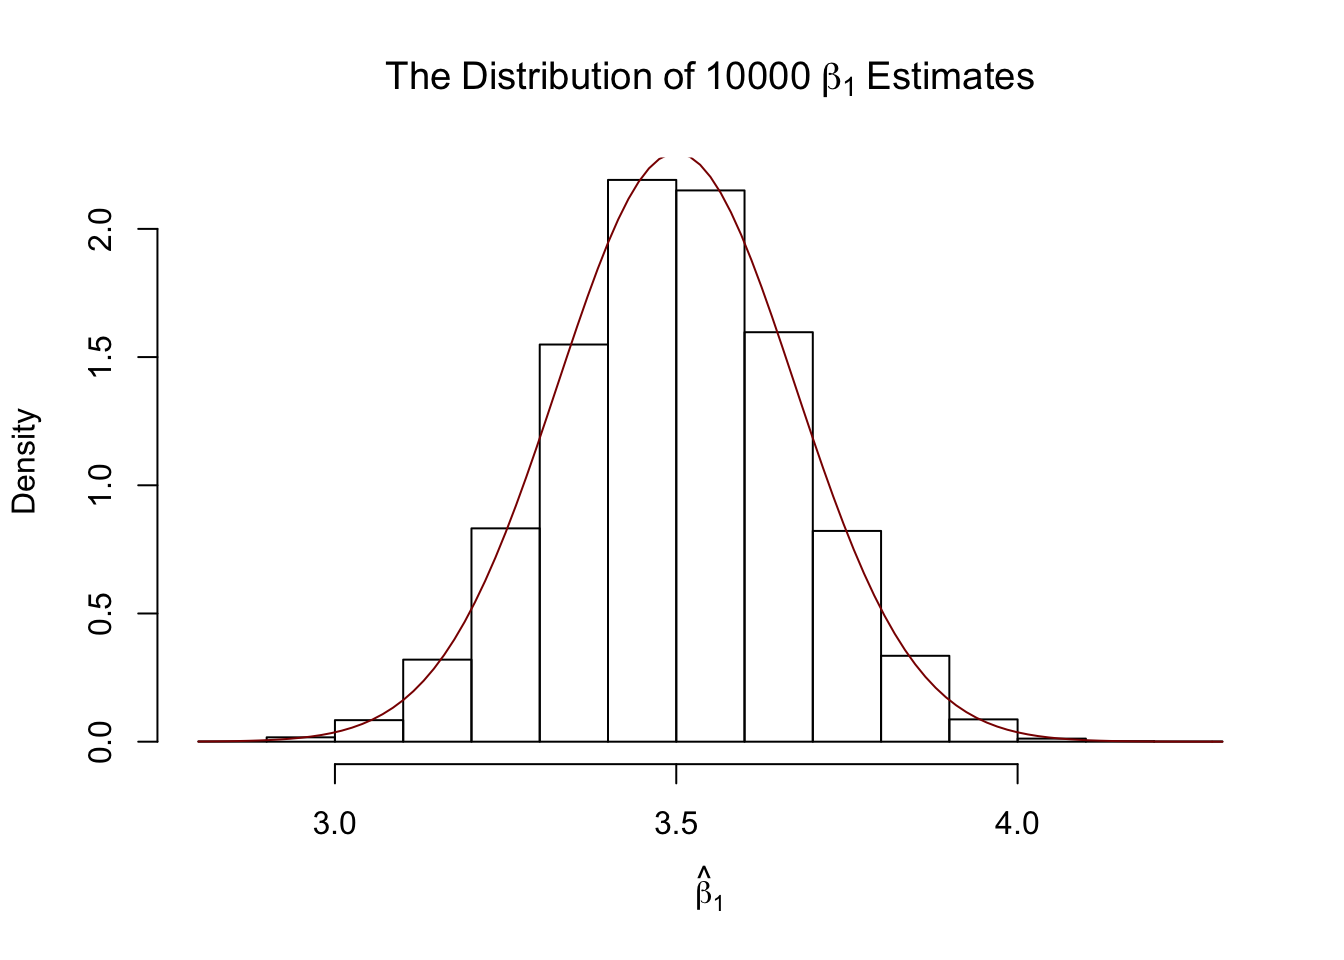
\includegraphics{URFITE_files/figure-latex/unnamed-chunk-92-2} \end{center}

We are now able to say the following: first, our variance estimates are
in favour of the claims made in Key Concept 4.4 since they come close to
the computed theoretical values. Second, the histograms suggest that the
estimators distributions indeed follow normal distributions which can be
fairly approximated by the respective normal distributions stated in Key
Concept 4.4.

\subsection*{R Simulation Study 2}\label{r-simulation-study-2}
\addcontentsline{toc}{subsection}{R Simulation Study 2}

A further result implied by Key Concept 4.4 is that both estimators are
consistent i.e.~they converge in probability to their true value. This
is since their variances converge to \(0\) as \(n\) increases. We can
check this by repeating the simulation above for an increasing sequence
of sample sizes. This means we no langer assign the sample size but a
\emph{vector} of sample sizes: \texttt{n\ \textless{}-\ c(...)}. Let us
look at the distributions of \(\beta_1\). The idea here is to add an
additional call of \texttt{for()} to the code. This is done in order to
loop over the vector of sample sizes \texttt{n}. For each of the sample
sizes we carry out the same simulation as before but plot a density
estimate for the outcomes of each iteration over \texttt{n}. Notice that
we have to change \texttt{n} to \texttt{n{[}j{]}} in the inner loop to
ensure that the \texttt{j}\(^{th}\) element of \texttt{n} is used. In
the simulation, we use sample sizes \(100, 250, 1000\) and \(3000\).
Consequently we have a total of four distinct simulations using
different sample sizes.

\begin{Shaded}
\begin{Highlighting}[]
\CommentTok{# set random seed for reproducibility}
\KeywordTok{set.seed}\NormalTok{(}\DecValTok{1}\NormalTok{)}

\CommentTok{# set repetitions and the vector of sample sizes}
\NormalTok{reps <-}\StringTok{ }\DecValTok{1000}
\NormalTok{n <-}\StringTok{ }\KeywordTok{c}\NormalTok{(}\DecValTok{100}\NormalTok{, }\DecValTok{250}\NormalTok{, }\DecValTok{1000}\NormalTok{, }\DecValTok{3000}\NormalTok{)}

\CommentTok{# initialize the matrix of outcomes}
\NormalTok{fit <-}\StringTok{ }\KeywordTok{matrix}\NormalTok{(}\DataTypeTok{ncol =} \DecValTok{2}\NormalTok{, }\DataTypeTok{nrow =}\NormalTok{ reps)}

\CommentTok{# devide the plot panel in a 2-by-2 array}
\KeywordTok{par}\NormalTok{(}\DataTypeTok{mfrow =} \KeywordTok{c}\NormalTok{(}\DecValTok{2}\NormalTok{,}\DecValTok{2}\NormalTok{))}

\NormalTok{#### Loop sampling and plotting ####}

\CommentTok{# outer loop over n}
\ControlFlowTok{for}\NormalTok{ (j }\ControlFlowTok{in} \DecValTok{1}\OperatorTok{:}\KeywordTok{length}\NormalTok{(n)) \{}
  
  \CommentTok{# inner loop: sampling and estimating of the coefficients}
  \ControlFlowTok{for}\NormalTok{ (i }\ControlFlowTok{in} \DecValTok{1}\OperatorTok{:}\NormalTok{reps)\{}
\NormalTok{    sample <-}\StringTok{ }\NormalTok{population[}\KeywordTok{sample}\NormalTok{(}\DecValTok{1}\OperatorTok{:}\NormalTok{N, n[j]), ]}
\NormalTok{    fit[i, ] <-}\StringTok{ }\KeywordTok{lm}\NormalTok{(Y }\OperatorTok{~}\StringTok{ }\NormalTok{X, }\DataTypeTok{data =}\NormalTok{ sample)}\OperatorTok{$}\NormalTok{coefficients}
\NormalTok{  \}}
  
  \CommentTok{# draw density estimates}
  \KeywordTok{plot}\NormalTok{(}\KeywordTok{density}\NormalTok{(fit[,}\DecValTok{2}\NormalTok{]), }\DataTypeTok{xlim=}\KeywordTok{c}\NormalTok{(}\FloatTok{2.5}\NormalTok{,}\FloatTok{4.5}\NormalTok{), }\DataTypeTok{col=}\NormalTok{j, }
       \DataTypeTok{main =} \KeywordTok{paste}\NormalTok{(}\StringTok{"n="}\NormalTok{, n[j]), }\DataTypeTok{xlab =} \KeywordTok{bquote}\NormalTok{(}\KeywordTok{hat}\NormalTok{(beta)[}\DecValTok{1}\NormalTok{]))}
  
\NormalTok{\}}
\end{Highlighting}
\end{Shaded}

\begin{center}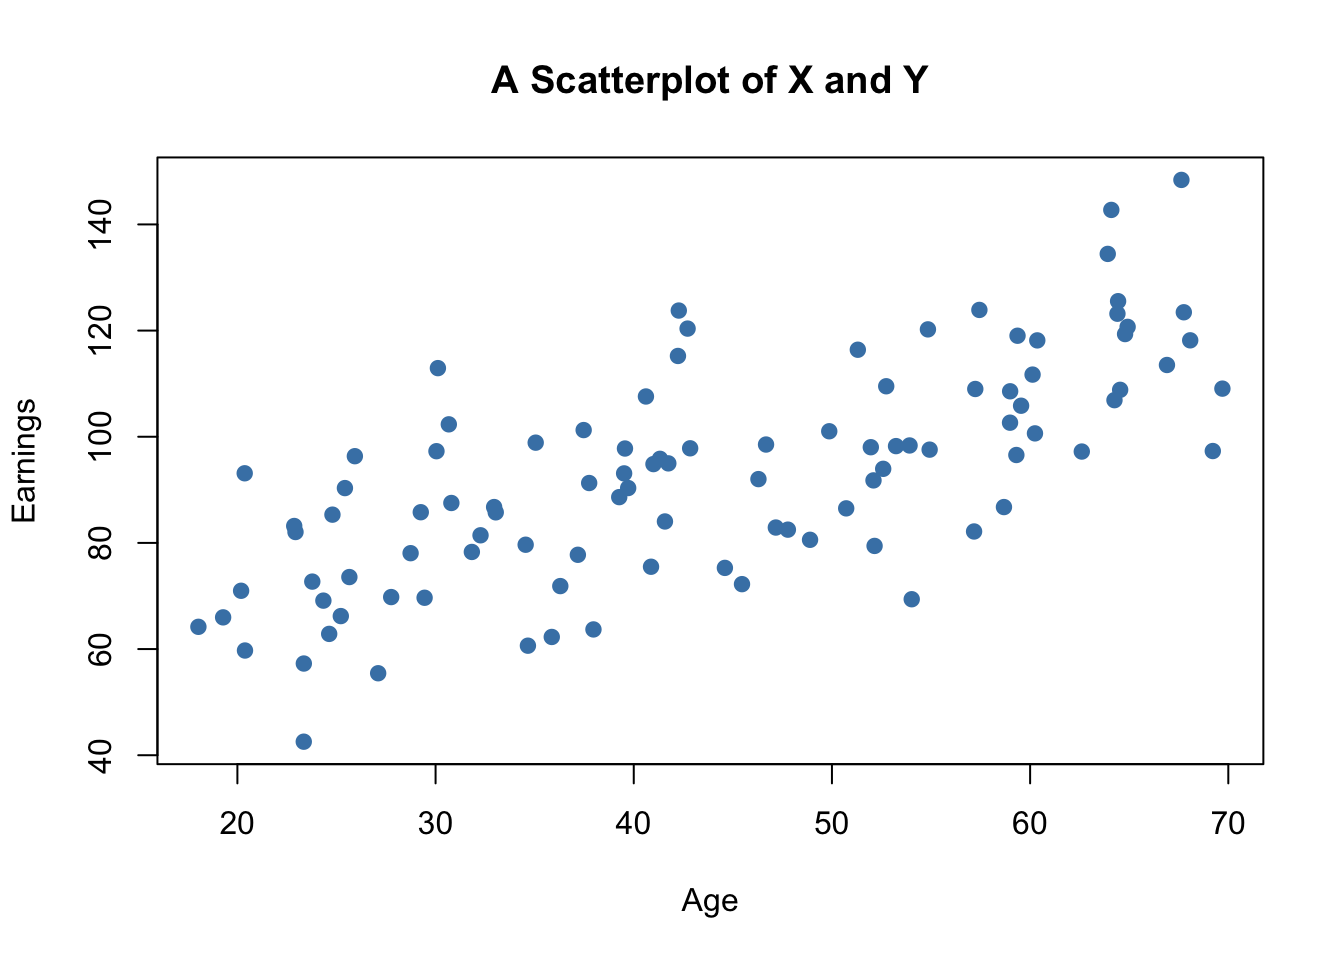
\includegraphics{URFITE_files/figure-latex/unnamed-chunk-93-1} \end{center}

We find that, as \(n\) increases, the distribution of \(\hat\beta_1\)
concentrates around its mean, i.e.~its variance decreases. Put
differently, the likelihood of observering estimates close to the true
value of \(\beta_1 = 3.5\) grows as we increase the sample size. The
same behaviour could be observed if we would analyze the distribution of
\(\hat\beta_0\) instead.

\subsection*{R Simulation Study 3}\label{r-simulation-study-3}
\addcontentsline{toc}{subsection}{R Simulation Study 3}

Furthermore, (4.1) reveals that the variance of the OLS estimator for
\(\beta_1\) decreases as the variance of the \(X_i\) increases. In other
words, as we increase the amount of information provided by the
regressor, that is increasing \(Var(X)\), which is used to estimate
\(\beta_1\), we are more confident that the estimate is close to the
true value (i.e. \(Var(\hat\beta_1)\) decreases). We can visualize this
by reproducing figure 4.6 from the book. To do this, we sample \(100\)
observations \((X,Y)\) from a bivariate normal distribution with

\[E(X)=E(Y)=5,\] \[Var(X)=Var(Y)=5\] and \[Cov(X,Y)=4.\]

Formally, this is written down as

\begin{align}
  \begin{pmatrix}
    X \\
    Y \\
  \end{pmatrix}
  \overset{i.i.d.}{\sim} & \ \mathcal{N} 
  \left[
    \begin{pmatrix}
      5 \\
      5 \\
    \end{pmatrix}, \ 
    \begin{pmatrix}
      5 & 4 \\
      4 & 5 \\
    \end{pmatrix}
  \right]. \tag{4.3}
\end{align}

To carry out the random sampling, we make use of the function
\texttt{mvtnorm()} from the package \texttt{MASS} which allows to draw
random samples from multivariate normal distributions, see
\texttt{?mvtnorm}. Next, we use the \texttt{subset()} function to split
the sample into two subsets such that the first set, \texttt{set1},
consists of observations that fulfill the condition
\(\lvert X - \overline{X} \rvert > 1\) and the second set,
\texttt{set2}, includes the remainder of the sample. We then plot both
sets and use different colors to make them distinguishable.

\begin{Shaded}
\begin{Highlighting}[]
\CommentTok{# load the MASS package}
\KeywordTok{library}\NormalTok{(MASS)}

\CommentTok{# set random seed for reproducibility}
\KeywordTok{set.seed}\NormalTok{(}\DecValTok{4}\NormalTok{)}

\CommentTok{# simulate bivarite normal data}
\NormalTok{bvndata <-}\StringTok{ }\KeywordTok{mvrnorm}\NormalTok{(}\DecValTok{100}\NormalTok{, }
                \DataTypeTok{mu =} \KeywordTok{c}\NormalTok{(}\DecValTok{5}\NormalTok{,}\DecValTok{5}\NormalTok{), }
                \DataTypeTok{Sigma =} \KeywordTok{cbind}\NormalTok{(}\KeywordTok{c}\NormalTok{(}\DecValTok{5}\NormalTok{,}\DecValTok{4}\NormalTok{),}\KeywordTok{c}\NormalTok{(}\DecValTok{4}\NormalTok{,}\DecValTok{5}\NormalTok{))}
\NormalTok{                ) }

\CommentTok{# assign column names / convert to data.frame}
\KeywordTok{colnames}\NormalTok{(bvndata) <-}\StringTok{ }\KeywordTok{c}\NormalTok{(}\StringTok{"X"}\NormalTok{,}\StringTok{"Y"}\NormalTok{)}
\NormalTok{bvndata <-}\StringTok{ }\KeywordTok{as.data.frame}\NormalTok{(bvndata)}

\CommentTok{# subset the data}
\NormalTok{set1 <-}\StringTok{ }\KeywordTok{subset}\NormalTok{(bvndata, }\KeywordTok{abs}\NormalTok{(}\KeywordTok{mean}\NormalTok{(X) }\OperatorTok{-}\StringTok{ }\NormalTok{X) }\OperatorTok{>}\StringTok{ }\DecValTok{1}\NormalTok{)}
\NormalTok{set2 <-}\StringTok{ }\KeywordTok{subset}\NormalTok{(bvndata, }\KeywordTok{abs}\NormalTok{(}\KeywordTok{mean}\NormalTok{(X) }\OperatorTok{-}\StringTok{ }\NormalTok{X) }\OperatorTok{<=}\StringTok{ }\DecValTok{1}\NormalTok{)}

\CommentTok{# plot both data sets}
\KeywordTok{plot}\NormalTok{(set1, }\DataTypeTok{xlab =} \StringTok{"X"}\NormalTok{, }\DataTypeTok{ylab =} \StringTok{"Y"}\NormalTok{, }\DataTypeTok{pch =} \DecValTok{19}\NormalTok{)}
\KeywordTok{points}\NormalTok{(set2, }\DataTypeTok{col =} \StringTok{"steelblue"}\NormalTok{, }\DataTypeTok{pch =} \DecValTok{19}\NormalTok{)}
\end{Highlighting}
\end{Shaded}

\begin{center}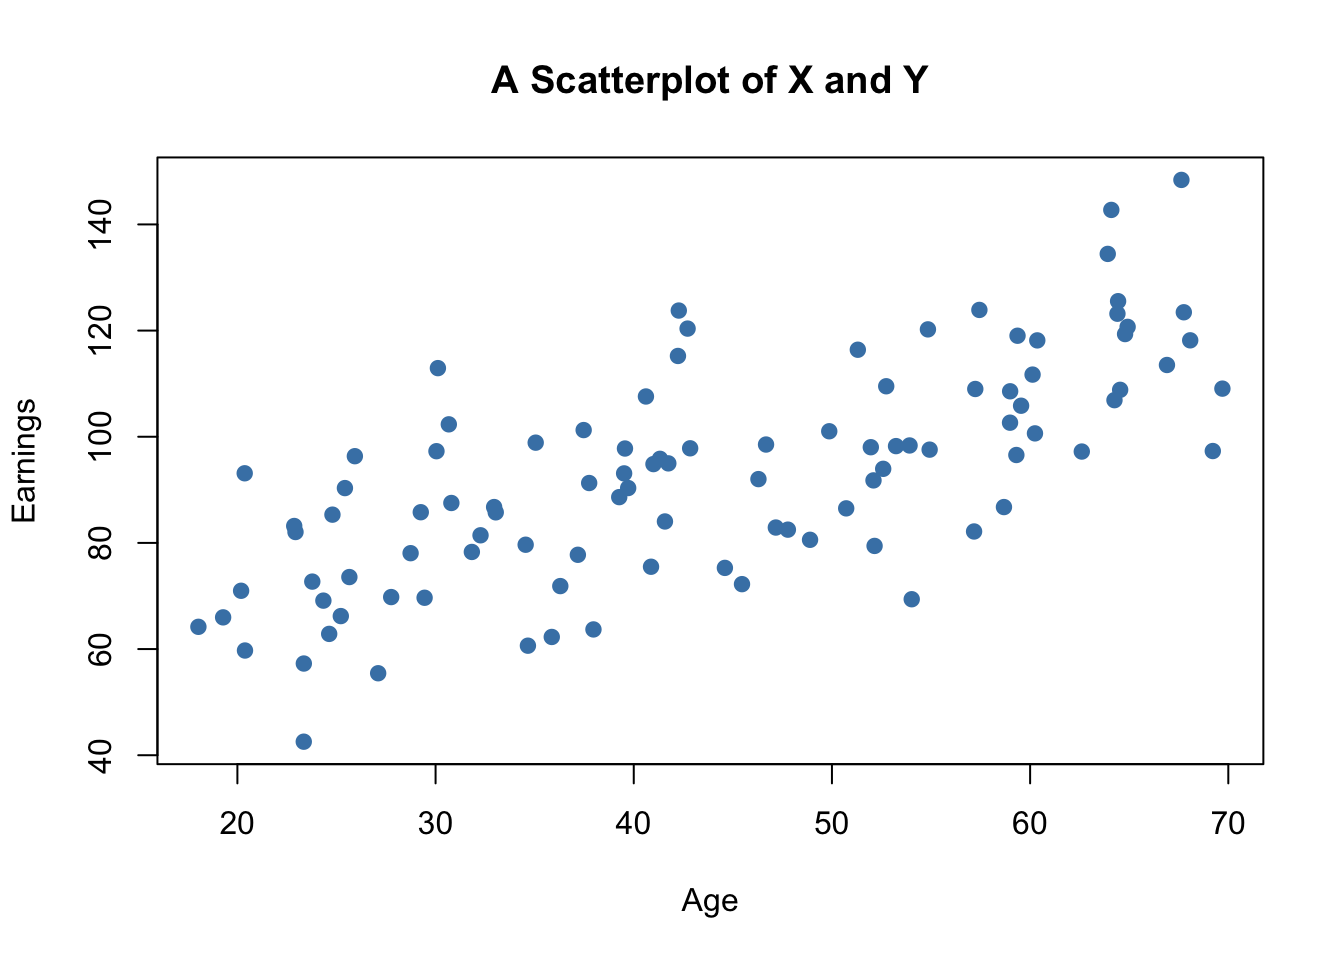
\includegraphics{URFITE_files/figure-latex/unnamed-chunk-94-1} \end{center}

It is clear that observations that are close to the sample average of
the \(X_i\) have less variance than those that are farther away. Now, if
we were to draw a line as accurately as possible through either of the
two sets it is obvious that choosing the observations indicated by the
black dots, i.e.~using the set of observations which has larger variance
than the blue ones, would result in a more precise line. Now, let us use
OLS to estimate and draw the regression lines for both sets of
observations.

\begin{Shaded}
\begin{Highlighting}[]
\CommentTok{# estimate both regression lines}
\NormalTok{lm.set1 <-}\StringTok{ }\KeywordTok{lm}\NormalTok{(Y }\OperatorTok{~}\StringTok{ }\NormalTok{X, }\DataTypeTok{data =}\NormalTok{ set1)}
\NormalTok{lm.set2 <-}\StringTok{ }\KeywordTok{lm}\NormalTok{(Y }\OperatorTok{~}\StringTok{ }\NormalTok{X, }\DataTypeTok{data =}\NormalTok{ set2)}

\CommentTok{# add both lines to the plot}
\KeywordTok{abline}\NormalTok{(lm.set1, }\DataTypeTok{col=}\StringTok{"green"}\NormalTok{)}
\KeywordTok{abline}\NormalTok{(lm.set2, }\DataTypeTok{col=}\StringTok{"red"}\NormalTok{)}
\end{Highlighting}
\end{Shaded}

\begin{center}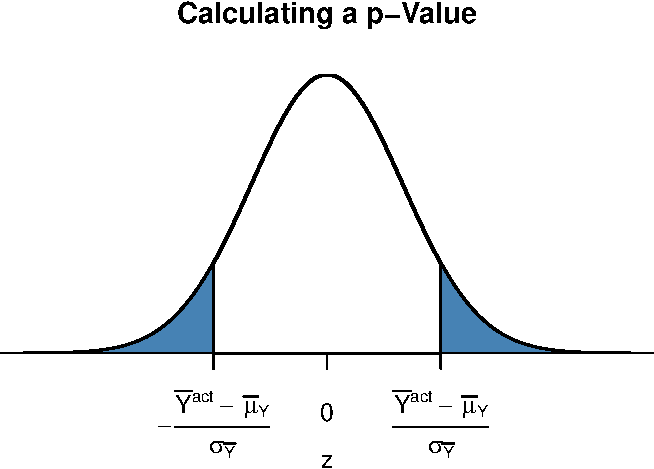
\includegraphics{URFITE_files/figure-latex/unnamed-chunk-95-1} \end{center}

Evidently, the green regression line does far better in describing data
sampled from the bivariate normal distribution stated in (4.3) than the
red line. This is a nice example why we are interested in a high
variance of the regressor \(X\): more variance in the \(X_i\) means more
information from which the precision of the estimation benefits.

\chapter{Hypothesis Tests and Confidence Intervals in the Simple Linear
Regression
Model}\label{hypothesis-tests-and-confidence-intervals-in-the-simple-linear-regression-model}

In this chapter, we continue with the treatment of the simple linear
regression model. The following subsction discuss how we may use our
knowledge about the sampling distribution of the OLS estimator in order
to make statements regarding its uncertainty. These subsections cover
the following topics:

\begin{itemize}
\item
  Testing Hypotheses about regression coefficients
\item
  Confidence intervals for regression coefficients
\item
  Regression when \(X\) is a dummy variable
\item
  Heteroskedasticity and Homoskedasticity
\end{itemize}

\section{\texorpdfstring{Testing Two-Sided Hypotheses Concerning
\(\beta_1\)}{Testing Two-Sided Hypotheses Concerning \textbackslash{}beta\_1}}\label{testing-two-sided-hypotheses-concerning-beta_1}

Using the fact that \(\hat{\beta}_1\) is approximately normal
distributed in large samples (see \protect\hyperlink{tsdotoe}{Key
Concept 4.4}), testing hypothesis about the true value \(\beta_1\) can
be done with the same approach as discussed in chapter 3.2.

Key Concept 5.1

General Form of the \(t\)-Statistic

Remember from chapter 3 that a general \(t\)-statistic has the form

\[
  t = \frac{\text{estimated value} - \text{hypothesized value}}{\text{standard error of the estimator}}.
\]

Key Concept 5.2

Testing Hyothesis about \(\beta_1\)

For testing the hypothesis \(H_0: \beta_1 = \beta_{1,0}\), we need to
perform the following steps:

\begin{enumerate}
\def\labelenumi{\arabic{enumi}.}
\tightlist
\item
  Compute the standard error of \(\hat{\beta}_1\), \(SE(\hat{\beta}_1)\)
\end{enumerate}

\[ SE(\hat{\beta}_1) = \sqrt{ \hat{\sigma}^2_{\hat{\beta}_1} } \ \ , \ \ 
  \hat{\sigma}^2_{\hat{\beta}_1} = \frac{1}{n} \times \frac{\frac{1}{n-2} \sum_{i=1}^n (X_i - \overline{X})^2 \hat{u_i}^2 }{ \left[ \frac{1}{n} \sum_{i=1}^n (X_i - \overline{X})^2 \right]^2}.
\]

\begin{enumerate}
\def\labelenumi{\arabic{enumi}.}
\setcounter{enumi}{1}
\tightlist
\item
  Compute the \(t\)-statistic
\end{enumerate}

\[ t = \frac{\hat{\beta}_1 - \beta_{1,0}}{ SE(\hat{\beta}_1) }. \]

\begin{enumerate}
\def\labelenumi{\arabic{enumi}.}
\setcounter{enumi}{2}
\tightlist
\item
  Now, given a two sided alternative (\(H_1:\beta_1 \neq \beta_{1,0}\))
  we reject at the \(5\%\) level if \(|t^{act}| > 1.96\) or,
  equivalently, if the \(p\)-value is less than \(0.05\).\\
  Recall the definition of the \(p\)-value:
\end{enumerate}

\begin{align}
    p \text{-value} =& \, \text{Pr}_{H_0} \left[ \left| \frac{ \hat{\beta}_1 - \beta_{1,0} }{ SE(\hat{\beta}_1) } \right| > \left|        \frac{ \hat{\beta}_1^{act} - \beta_{1,0} }{ SE(\hat{\beta}_1) } \right| \right] \\
    =& \, \text{Pr}_{H_0} (|t| > |t^{act}|) \\
    =& \, 2 \cdot \Phi(-|t^{act}|)
  \end{align}

~~~~~~ The last equality holds due to the normal approximation for large
samples.

Consider again the OLS regression stored in \texttt{linear\_model} from
Chapter 4 that gave us the regression line

\[ \widehat{TestScore} \ = \underset{(9.47)}{698.9} - \underset{(0.49)}{2.28} \times STR \ , \ R^2=0.051 \ , \ SER=18.6. \]

For testing a hypothesis about the slope parameter (the coefficient on
\(STR\)), we need \(SE(\hat{\beta}_1)\), the standard error of the
respective point estimator. As common in the literature, standard errors
are presented in parantheses below the point estimates.

As can be witnessed in Key Concept 5.1 it is rather cumbersome to
compute the standard error and thus the \(t\)-statistic by hand. The
question You should be asking Yourself right now is obvious: can we
obtain these values with minimum effort using R? Yes, we can. Let us
first use \texttt{summary()} to get a summary on the estimated
coefficients in \texttt{linear\_model}.

\begin{Shaded}
\begin{Highlighting}[]
\CommentTok{# print the summary of coefficients to the console}
\KeywordTok{summary}\NormalTok{(linear_model)}\OperatorTok{$}\NormalTok{coefficients}
\end{Highlighting}
\end{Shaded}

\begin{verbatim}
##               Estimate Std. Error   t value      Pr(>|t|)
## (Intercept) 698.932949  9.4674911 73.824516 6.569846e-242
## STR          -2.279808  0.4798255 -4.751327  2.783308e-06
\end{verbatim}

When looking at the second column of the coefficients' summary, we
discover values for \(SE(\hat\beta_0)\) and \(SE(\hat\beta_1)\). Also,
in the third column, named \texttt{t\ value}, we find \(t\)-statistics
\(t^{act}\) suitable for tests of the individual hypotheses
\(H_0: \beta_0=0\) and \(H_0: \beta_1=0\). Furthermore, the output
provides us with \(p\)-values corresponding to both tests against the
two-sided alternatives \(H_1:\beta_0\neq0\) respectively
\(H_1:\beta_1\neq0\) in the fourth column of the table.

Let us have a closer look at the test of

\[H_0: \beta_1=0 \ \ \ vs. \ \ \ H_1: \beta_1 \neq 0.\]

Using our revisited knowledge about \(t\)-statistics we find that

\[ t^{act} = \frac{-2.279808 - 0}{0.4798255} \approx - 4.75. \]

What does this tell us about the significance of the estimated
coefficient? We reject the null hypothesis at the \(5\%\) level of
significance since \(|t^{act}| > 1.96\) that is the observed test
statistic falls into the region of rejection. Or, alternatively and
leading to the same result, we have
\(p\text{-value} = 2.78*10^{-6} < 0.05\). We conclude that the
coefficient is significantly different from zero. With other words, our
analysis provides evidence that the clase size \emph{has an influence}
on the students test scores. We say that \(\beta_1\) is significantly
different from \(0\) at the level of \(5\%\).

Note that, although the difference is negligible in the present case as
we will see later, \texttt{summary()} does not perform the normal
approximation but calculates \(p\)-values using the appropriate
\(t\)-distribution instead. Generally, the degrees of freedom are
determined in the following manner:

\[ \text{DF} = n - k - 1 \]

where \(n\) is the number of observations used to estimate the model and
\(k\) is the number of regressors, excluding the intercept. In our case,
we have \(n=420\) observations and the only regressor is \(STR\) so
\(k=1\). A sleek way to determine the model degress of freedom using R
is

\begin{Shaded}
\begin{Highlighting}[]
\CommentTok{# determine degrees of freedom}
\NormalTok{linear_model}\OperatorTok{$}\NormalTok{df.residual}
\end{Highlighting}
\end{Shaded}

\begin{verbatim}
## [1] 418
\end{verbatim}

Hence, for the sampling distribution of \(\hat\beta_1\) we have

\[ \hat\beta_1 \sim t_{418}\] such that the \(p\)-value for a two-sided
significance test can be obtained by executing the following code:

\begin{Shaded}
\begin{Highlighting}[]
\DecValTok{2} \OperatorTok{*}\StringTok{ }\KeywordTok{pt}\NormalTok{(}\OperatorTok{-}\FloatTok{4.751327}\NormalTok{, }\DataTypeTok{df =} \DecValTok{418}\NormalTok{)}
\end{Highlighting}
\end{Shaded}

\begin{verbatim}
## [1] 2.78331e-06
\end{verbatim}

The result is very close to the value provided by \texttt{summary}.
However since \(n\) is sufficiently large one could just as well use the
standard normal density to compute the \(p\)-value:

\begin{Shaded}
\begin{Highlighting}[]
\DecValTok{2} \OperatorTok{*}\StringTok{ }\KeywordTok{pnorm}\NormalTok{(}\OperatorTok{-}\FloatTok{4.751327}\NormalTok{)}
\end{Highlighting}
\end{Shaded}

\begin{verbatim}
## [1] 2.02086e-06
\end{verbatim}

The difference is indeed negligible. These findings tell us that, if
\(H_0: \beta_1 = 0\) is true and we were to repeat the whole process of
gathering observations and estimating the model, chances of observing a
\(\hat\beta_1 \geq |-4.75|\) are roughly \(1:359285\) --- so higher
chances than winning the lottory next saturday but still very unlikely!

Using R we may visualise how such a statement is made when using the
normal approximation. This reflects the principles depicted in figure
5.1 in the book. Do not let the following code chunk deter You: the code
is somewhat longer than the usual examples and looks unappealing but
there is \textbf{a lot} of repetition since color shadings and
annotations are added on both tails of the normal distribution. We
recommend You to execute the code step by step in order to see how the
graph is augmented with the annotations.

\begin{Shaded}
\begin{Highlighting}[]
\CommentTok{# Plot the standard normal on the domain [-6,6]}
\NormalTok{t <-}\StringTok{ }\KeywordTok{seq}\NormalTok{(}\OperatorTok{-}\DecValTok{6}\NormalTok{,}\DecValTok{6}\NormalTok{,}\FloatTok{0.01}\NormalTok{)}

\KeywordTok{plot}\NormalTok{(}\DataTypeTok{x =}\NormalTok{ t, }
     \DataTypeTok{y =} \KeywordTok{dnorm}\NormalTok{(t, }\DecValTok{0}\NormalTok{, }\DecValTok{1}\NormalTok{), }
     \DataTypeTok{type =} \StringTok{"l"}\NormalTok{, }
     \DataTypeTok{col =} \StringTok{"steelblue"}\NormalTok{, }
     \DataTypeTok{lwd =} \DecValTok{2}\NormalTok{, }
     \DataTypeTok{yaxs =} \StringTok{"i"}\NormalTok{, }
     \DataTypeTok{axes =}\NormalTok{ F, }
     \DataTypeTok{ylab =} \StringTok{""}\NormalTok{, }
     \DataTypeTok{main =} \StringTok{"Calculating the p-Value of a Two-Sided Test When t^act = -4.75"}\NormalTok{, }
     \DataTypeTok{cex.lab =} \FloatTok{0.7}
\NormalTok{     )}

\NormalTok{tact <-}\StringTok{ }\OperatorTok{-}\FloatTok{4.75}

\KeywordTok{axis}\NormalTok{(}\DecValTok{1}\NormalTok{, }\DataTypeTok{at =} \KeywordTok{c}\NormalTok{(}\DecValTok{0}\NormalTok{,}\OperatorTok{-}\FloatTok{1.96}\NormalTok{,}\FloatTok{1.96}\NormalTok{,}\OperatorTok{-}\NormalTok{tact,tact), }\DataTypeTok{cex.axis=}\FloatTok{0.7}\NormalTok{)}

\CommentTok{# Shade the critical regions using polygon()}

\NormalTok{## critical region in left tail}
\KeywordTok{polygon}\NormalTok{(}\DataTypeTok{x =} \KeywordTok{c}\NormalTok{(}\OperatorTok{-}\DecValTok{6}\NormalTok{, }\KeywordTok{seq}\NormalTok{(}\OperatorTok{-}\DecValTok{6}\NormalTok{,}\OperatorTok{-}\FloatTok{1.96}\NormalTok{,}\FloatTok{0.01}\NormalTok{),}\OperatorTok{-}\FloatTok{1.96}\NormalTok{),}
        \DataTypeTok{y =} \KeywordTok{c}\NormalTok{(}\DecValTok{0}\NormalTok{, }\KeywordTok{dnorm}\NormalTok{(}\KeywordTok{seq}\NormalTok{(}\OperatorTok{-}\DecValTok{6}\NormalTok{,}\OperatorTok{-}\FloatTok{1.96}\NormalTok{,}\FloatTok{0.01}\NormalTok{)),}\DecValTok{0}\NormalTok{), }
        \DataTypeTok{col =} \StringTok{'orange'}
\NormalTok{        )}

\NormalTok{## critical region in right tail}

\KeywordTok{polygon}\NormalTok{(}\DataTypeTok{x =} \KeywordTok{c}\NormalTok{(}\FloatTok{1.96}\NormalTok{, }\KeywordTok{seq}\NormalTok{(}\FloatTok{1.96}\NormalTok{, }\DecValTok{6}\NormalTok{, }\FloatTok{0.01}\NormalTok{), }\DecValTok{6}\NormalTok{),}
        \DataTypeTok{y =} \KeywordTok{c}\NormalTok{(}\DecValTok{0}\NormalTok{, }\KeywordTok{dnorm}\NormalTok{(}\KeywordTok{seq}\NormalTok{(}\FloatTok{1.96}\NormalTok{, }\DecValTok{6}\NormalTok{, }\FloatTok{0.01}\NormalTok{)), }\DecValTok{0}\NormalTok{), }
        \DataTypeTok{col =} \StringTok{'orange'}
\NormalTok{        )}

\CommentTok{# Add arrows and texts indicating critical regions and the p-value}
\KeywordTok{arrows}\NormalTok{(}\OperatorTok{-}\FloatTok{3.5}\NormalTok{, }\FloatTok{0.2}\NormalTok{, }\OperatorTok{-}\FloatTok{2.5}\NormalTok{, }\FloatTok{0.02}\NormalTok{, }\DataTypeTok{length =} \FloatTok{0.1}\NormalTok{)}
\KeywordTok{arrows}\NormalTok{(}\FloatTok{3.5}\NormalTok{, }\FloatTok{0.2}\NormalTok{, }\FloatTok{2.5}\NormalTok{, }\FloatTok{0.02}\NormalTok{, }\DataTypeTok{length =} \FloatTok{0.1}\NormalTok{)}

\KeywordTok{arrows}\NormalTok{(}\OperatorTok{-}\DecValTok{5}\NormalTok{, }\FloatTok{0.16}\NormalTok{, }\OperatorTok{-}\FloatTok{4.75}\NormalTok{, }\DecValTok{0}\NormalTok{, }\DataTypeTok{length =} \FloatTok{0.1}\NormalTok{)}
\KeywordTok{arrows}\NormalTok{(}\DecValTok{5}\NormalTok{, }\FloatTok{0.16}\NormalTok{, }\FloatTok{4.75}\NormalTok{, }\DecValTok{0}\NormalTok{, }\DataTypeTok{length =} \FloatTok{0.1}\NormalTok{)}

\KeywordTok{text}\NormalTok{(}\OperatorTok{-}\FloatTok{3.5}\NormalTok{,}\FloatTok{0.22}\NormalTok{, }\DataTypeTok{labels =} \KeywordTok{paste}\NormalTok{(}\StringTok{"0.025="}\NormalTok{,}\KeywordTok{expression}\NormalTok{(alpha),}\StringTok{"/2"}\NormalTok{,}\DataTypeTok{sep =} \StringTok{""}\NormalTok{), }\DataTypeTok{cex =} \FloatTok{0.7}\NormalTok{)}
\KeywordTok{text}\NormalTok{(}\FloatTok{3.5}\NormalTok{,}\FloatTok{0.22}\NormalTok{, }\DataTypeTok{labels =} \KeywordTok{paste}\NormalTok{(}\StringTok{"0.025="}\NormalTok{,}\KeywordTok{expression}\NormalTok{(alpha),}\StringTok{"/2"}\NormalTok{,}\DataTypeTok{sep =} \StringTok{""}\NormalTok{), }\DataTypeTok{cex =} \FloatTok{0.7}\NormalTok{)}

\KeywordTok{text}\NormalTok{(}\OperatorTok{-}\DecValTok{5}\NormalTok{,}\FloatTok{0.18}\NormalTok{, }\DataTypeTok{labels =} \KeywordTok{expression}\NormalTok{(}\KeywordTok{paste}\NormalTok{(}\StringTok{"-|"}\NormalTok{,t[act],}\StringTok{"|"}\NormalTok{)), }\DataTypeTok{cex =} \FloatTok{0.7}\NormalTok{)}
\KeywordTok{text}\NormalTok{(}\DecValTok{5}\NormalTok{,}\FloatTok{0.18}\NormalTok{, }\DataTypeTok{labels =} \KeywordTok{expression}\NormalTok{(}\KeywordTok{paste}\NormalTok{(}\StringTok{"|"}\NormalTok{,t[act],}\StringTok{"|"}\NormalTok{)), }\DataTypeTok{cex =} \FloatTok{0.7}\NormalTok{)}

\CommentTok{# Add ticks indicating critical values at the 0.05-level, t^act and -t^act }
\KeywordTok{rug}\NormalTok{(}\KeywordTok{c}\NormalTok{(}\OperatorTok{-}\FloatTok{1.96}\NormalTok{,}\FloatTok{1.96}\NormalTok{), }\DataTypeTok{ticksize  =} \FloatTok{0.145}\NormalTok{, }\DataTypeTok{lwd =} \DecValTok{2}\NormalTok{, }\DataTypeTok{col =} \StringTok{"darkred"}\NormalTok{)}
\KeywordTok{rug}\NormalTok{(}\KeywordTok{c}\NormalTok{(}\OperatorTok{-}\NormalTok{tact,tact), }\DataTypeTok{ticksize  =} \OperatorTok{-}\FloatTok{0.0451}\NormalTok{, }\DataTypeTok{lwd =} \DecValTok{2}\NormalTok{, }\DataTypeTok{col =} \StringTok{"darkgreen"}\NormalTok{)}
\end{Highlighting}
\end{Shaded}

\begin{center}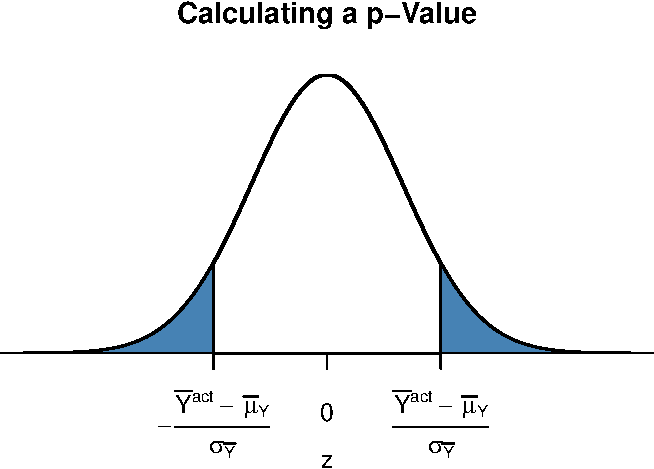
\includegraphics{URFITE_files/figure-latex/unnamed-chunk-100-1} \end{center}

The \(p\)-Value is the area under the curve to left of \(-4.75\) plus
the area under the curve to the right of \(4.75\). As we already know
from the calculations above, this value is very small.

\section{Confidence Intervals for Regression
Coefficients}\label{confidence-intervals-for-regression-coefficients}

As we already know, estimates of the regression coefficients \(\beta_0\)
and \(\beta_1\) are afflicted with sampling uncertainty, see chapter 4.
Therefore, we will \emph{never} estimate the exact true value of these
parameters from sample data in an empirical application. However, we may
construct confidence intervals for the intercept and the slope
parameter.

A \(95\%\) confidence interval for \(\beta_i\) has two equivalent
definitions:

\begin{itemize}
\tightlist
\item
  The interval is the set of values for which a hypothesis test to the
  level of \(5\%\) cannot be rejected.
\item
  The interval has a probability of \(95\%\) to contain the true value
  of \(\beta_i\). So in \(95\%\) of all samples that could be drawn, the
  confidence interval will cover the true value of \(\beta_i\).
\end{itemize}

We also say that the interval has a confidence level of \(95\%\). The
idea is summarized in Key Concept 5.3.

Key Concept 5.3

A Confidence Interval for \(\beta_i\)

Imagine You could draw all possible random samples of given size. The
interval that contains the true value \(\beta_i\) in \(95\%\) of all
samples is given by the expression

\[ \text{KI}_{0.95}^{\beta_i} = \left[ \hat{\beta}_i - 1.96 \times SE(\hat{\beta}_i) \, , \, \hat{\beta}_i + 1.96 \times SE(\hat{\beta}_i) \right]. \]

Equivalently, this interval can be seen as the set of null hypotheses
for which a \(5\%\) two-sided hypothesis test does not reject.

\subsection*{R Simulation Study 5.1}\label{r-simulation-study-5.1}
\addcontentsline{toc}{subsection}{R Simulation Study 5.1}

To get a better understanding of confidence intervalls we will conduct
another simulation study. For now, assume that we are confronted with
the following sample of \(n=100\) observations on a single variable
\(Y\) where

\[ Y_i \overset{i.i.d}{\sim} N(5,25) \ \ \forall \ i = 1, \dots, 100.\]

\begin{Shaded}
\begin{Highlighting}[]
\CommentTok{# set random seed for reproducibility}
\KeywordTok{set.seed}\NormalTok{(}\DecValTok{4}\NormalTok{)}

\CommentTok{# generate and plot the sample data}
\NormalTok{Y <-}\StringTok{ }\KeywordTok{rnorm}\NormalTok{(}\DataTypeTok{n =} \DecValTok{100}\NormalTok{, }
           \DataTypeTok{mean =} \DecValTok{5}\NormalTok{, }
           \DataTypeTok{sd =}\DecValTok{5}
\NormalTok{           )}

\KeywordTok{plot}\NormalTok{(Y, }
     \DataTypeTok{pch=}\DecValTok{19}\NormalTok{, }
     \DataTypeTok{col =} \StringTok{"steelblue"}
\NormalTok{     )}
\end{Highlighting}
\end{Shaded}

\begin{center}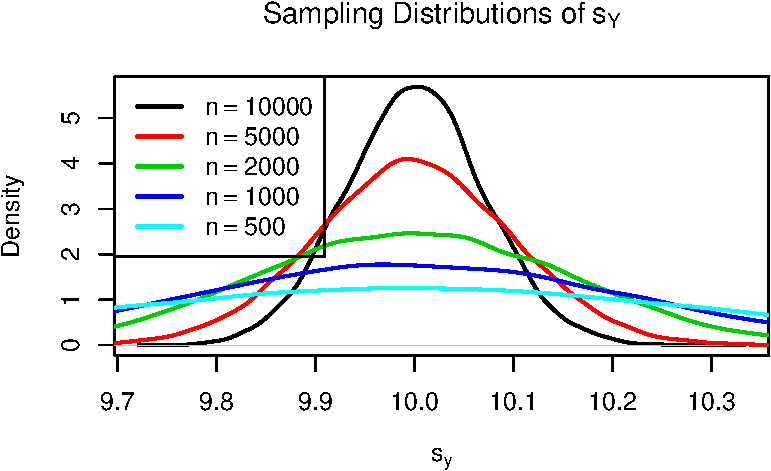
\includegraphics{URFITE_files/figure-latex/unnamed-chunk-101-1} \end{center}

We assume that the data is generated by the model

\[ Y_i = \mu + \epsilon_i \]

where \(\mu\) is the unknown constant and we know that
\(\epsilon_i \overset{i.i.d.}{\sim} N(0,25)\). In this model, the OLS
estimator for \(\mu\) is given by

\[ \hat\mu = \overline{Y} = \frac{1}{n} \sum_{i=1}^n Y_i \]

(try to verify this!) i.e.~the sample average of the \(Y_i\). It further
holds that

\[ SE(\hat\mu) = \frac{\sigma_{\epsilon}}{\sqrt{n}} = \frac{5}{\sqrt{100}}. \]

A large sample \(95\%\) confidence intervall for \(\mu\) is then given
by

\begin{equation} 
KI^{\mu}_{0.95} = \left[\hat\mu - 1.96 \times \frac{5}{\sqrt{100}} \ , \ \hat\mu + 1.96 \times \frac{5}{\sqrt{100}}  \right]. \label{eq:KI}
\end{equation}

It is fairly easy to compute this interval in R by hand. The following
code chunck generates a named vector containing the interval bounds:

\begin{Shaded}
\begin{Highlighting}[]
\KeywordTok{cbind}\NormalTok{(}
  \DataTypeTok{CIlower =} \KeywordTok{mean}\NormalTok{(Y) }\OperatorTok{-}\StringTok{ }\FloatTok{1.96} \OperatorTok{*}\StringTok{ }\DecValTok{5}\OperatorTok{/}\DecValTok{10}\NormalTok{, }
  \DataTypeTok{CIupper =} \KeywordTok{mean}\NormalTok{(Y) }\OperatorTok{+}\StringTok{ }\FloatTok{1.96} \OperatorTok{*}\StringTok{ }\DecValTok{5}\OperatorTok{/}\DecValTok{10} 
\NormalTok{)}
\end{Highlighting}
\end{Shaded}

\begin{verbatim}
##       CIlower  CIupper
## [1,] 4.502625 6.462625
\end{verbatim}

Nowing that \(\mu = 5\) we see that our example covers the true value
for the present sample. As opposed to real world examples, we can use R
to get a better understanding of confidence intervals by repeatedly
sampling data, estimating \(\mu\) and computing the confidence interval
for \(\mu\) as in \eqref{eq:KI}.

The procedure is as follows:

\begin{itemize}
\tightlist
\item
  We initialize the vectors \texttt{lower} and \texttt{upper} in which
  the simulated interval boundaries are to be saved. We want to simulate
  \(10000\) intervals so both vectors are set to have this length.
\item
  We use a \texttt{for()} loop to sample \(100\) observations from the
  \(N(5,25)\) distribution and compute \(\hat\mu\) as well as the
  boundaries of the confidence interval in every iteration of the loop.
\item
  At last we join \texttt{lower} and \texttt{upper} in an array.
\end{itemize}

\begin{Shaded}
\begin{Highlighting}[]
\CommentTok{# set random seed}
\KeywordTok{set.seed}\NormalTok{(}\DecValTok{1}\NormalTok{)}

\CommentTok{# initialize vectors of lower and upper interval boundaries}
\NormalTok{lower <-}\StringTok{ }\KeywordTok{numeric}\NormalTok{(}\DecValTok{10000}\NormalTok{)}
\NormalTok{upper <-}\StringTok{ }\KeywordTok{numeric}\NormalTok{(}\DecValTok{10000}\NormalTok{)}

\CommentTok{# loop sampling / estimation / CI}
\ControlFlowTok{for}\NormalTok{(i }\ControlFlowTok{in} \DecValTok{1}\OperatorTok{:}\DecValTok{10000}\NormalTok{) \{}
\NormalTok{  Y <-}\StringTok{ }\KeywordTok{rnorm}\NormalTok{(}\DecValTok{100}\NormalTok{, }\DataTypeTok{mean =} \DecValTok{5}\NormalTok{, }\DataTypeTok{sd =}\DecValTok{5}\NormalTok{)}
\NormalTok{  lower[i] <-}\StringTok{ }\KeywordTok{mean}\NormalTok{(Y) }\OperatorTok{-}\StringTok{ }\FloatTok{1.96} \OperatorTok{*}\StringTok{ }\DecValTok{5}\OperatorTok{/}\DecValTok{10}
\NormalTok{  upper[i] <-}\StringTok{ }\KeywordTok{mean}\NormalTok{(Y) }\OperatorTok{+}\StringTok{ }\FloatTok{1.96} \OperatorTok{*}\StringTok{ }\DecValTok{5}\OperatorTok{/}\DecValTok{10}
\NormalTok{\}}

\CommentTok{# join vectors of interval boundaries}
\NormalTok{CIs <-}\StringTok{ }\KeywordTok{cbind}\NormalTok{(lower, upper)}
\end{Highlighting}
\end{Shaded}

According to Key Concept 5.3 we expect that the fraction of the
\(10000\) simulated intervals saved in the array \texttt{CIs} that
contain the true value \(\mu=5\) should be roughly \(95\%\). We can
check this using logical operators.

\begin{Shaded}
\begin{Highlighting}[]
\KeywordTok{sum}\NormalTok{(CIs[,}\DecValTok{1}\NormalTok{] }\OperatorTok{<=}\StringTok{ }\DecValTok{5} \OperatorTok{&}\StringTok{ }\DecValTok{5} \OperatorTok{<=}\StringTok{ }\NormalTok{CIs[,}\DecValTok{2}\NormalTok{])}\OperatorTok{/}\DecValTok{10000}
\end{Highlighting}
\end{Shaded}

\begin{verbatim}
## [1] 0.9487
\end{verbatim}

The simulation shows that the fraction of intervals covering \(\mu=5\),
i.e.~those intervals for which \(H_0: \mu = 5\) cannot be rejected is
close to the theoretical value of \(95\%\).

Let us draw a plot of the first \(100\) simulated confidence intervals
and indicate those which \emph{do not} cover the true value of \(\mu\).
We do this by adding horizonal lines representing the confidence
intervals on top of each other.

\begin{Shaded}
\begin{Highlighting}[]
\CommentTok{# identify intervals not covering mu}
\CommentTok{# (4 intervals out of 100)}
\NormalTok{ID <-}\StringTok{ }\KeywordTok{which}\NormalTok{(}\OperatorTok{!}\NormalTok{(CIs[}\DecValTok{1}\OperatorTok{:}\DecValTok{100}\NormalTok{,}\DecValTok{1}\NormalTok{] }\OperatorTok{<=}\StringTok{ }\DecValTok{5} \OperatorTok{&}\StringTok{ }\DecValTok{5} \OperatorTok{<=}\StringTok{ }\NormalTok{CIs[}\DecValTok{1}\OperatorTok{:}\DecValTok{100}\NormalTok{,}\DecValTok{2}\NormalTok{]))}

\CommentTok{# initialize the plot}
\KeywordTok{plot}\NormalTok{(}\DecValTok{0}\NormalTok{, }
     \DataTypeTok{xlim =} \KeywordTok{c}\NormalTok{(}\DecValTok{3}\NormalTok{,}\DecValTok{7}\NormalTok{), }
     \DataTypeTok{ylim =} \KeywordTok{c}\NormalTok{(}\DecValTok{1}\NormalTok{,}\DecValTok{100}\NormalTok{), }
     \DataTypeTok{ylab =} \StringTok{"Sample"}\NormalTok{, }
     \DataTypeTok{xlab =} \KeywordTok{expression}\NormalTok{(mu), }
     \DataTypeTok{main =} \StringTok{"Confidence Intervals: Correct H0"}\NormalTok{)}

\CommentTok{# setup color vector}
\NormalTok{colors <-}\StringTok{ }\KeywordTok{rep}\NormalTok{(}\KeywordTok{gray}\NormalTok{(}\FloatTok{0.6}\NormalTok{), }\DecValTok{100}\NormalTok{)}
\NormalTok{colors[ID] <-}\StringTok{ "red"}

\CommentTok{# draw reference line at mu=5}
\KeywordTok{abline}\NormalTok{(}\DataTypeTok{v=}\DecValTok{5}\NormalTok{, }\DataTypeTok{lty=}\DecValTok{2}\NormalTok{)}

\CommentTok{# add horizontal bars representing the CIs}
\ControlFlowTok{for}\NormalTok{(j }\ControlFlowTok{in} \DecValTok{1}\OperatorTok{:}\DecValTok{100}\NormalTok{) \{}
  \KeywordTok{lines}\NormalTok{(}\KeywordTok{c}\NormalTok{(CIs[j,}\DecValTok{1}\NormalTok{], CIs[j,}\DecValTok{2}\NormalTok{]), }
        \KeywordTok{c}\NormalTok{(j,j), }
        \DataTypeTok{col =}\NormalTok{ colors[j], }
        \DataTypeTok{lwd=}\DecValTok{2}\NormalTok{)}
\NormalTok{\}}
\end{Highlighting}
\end{Shaded}

\begin{center}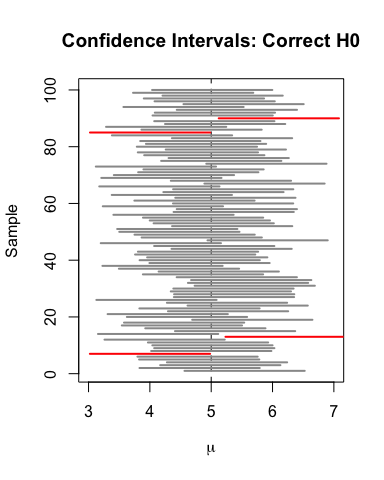
\includegraphics{URFITE_files/figure-latex/unnamed-chunk-105-1} \end{center}

We find that for the first 100 samples, the true null hypthesis is
rejected in four cases so these intervals do not cover \(\mu=5\). We
have indicated the intervals which lead to a rejection of the true null
hypothesis by red color.

Let us now turn back to the example of test scores and class sizes.The
regression model from chapter 4 is stored in \texttt{linear\_model}. An
easy way to get \(95\%\) confidence intervals for \(\beta_0\) and
\(\beta_1\), the coefficients on \texttt{(intercept)} and \texttt{STR},
is to use the function \texttt{confint()}. We only have to provide a
fitted model object as the argument \texttt{object} to this function.
The confidence level is set to \(95\%\) by default but can be modified
by setting the argument \texttt{level}, see \texttt{?confint}.

\begin{Shaded}
\begin{Highlighting}[]
\KeywordTok{confint}\NormalTok{(}\DataTypeTok{object =}\NormalTok{ linear_model)}
\end{Highlighting}
\end{Shaded}

\begin{verbatim}
##                 2.5 %     97.5 %
## (Intercept) 680.32312 717.542775
## STR          -3.22298  -1.336636
\end{verbatim}

Let us check if the calculation is done as we expect it to be. For
\(\beta_1\), that is the coefficient on \texttt{STR}, according to the
formula presented above the interval borders are computed as

\[  -2.279808 \pm 1.96 \times 0.4798255 \, \Rightarrow \, \text{KI}_{0.95}^{\beta_1} = \left[ -3.22, -1.34 \right]  \]

so this actually leads to the same interval. Obviously, this interval
\emph{does not} contain the value zero what, as we have already seen in
the previous section, leads to rejection of the null hypothesis
\(\beta_{1,0} = 0\).

\section{\texorpdfstring{Regression when \(X\) is a Binary
Variable}{Regression when X is a Binary Variable}}\label{regression-when-x-is-a-binary-variable}

Instead of using a continuous regressor \(X\), we might be interested in
running the regression

\[ Y_i = \beta_0 + \beta_1 D_i + u_i \tag{5.2} \]

where \(D_i\) is binary variable, a so-called \emph{dummy variable}. For
example, we may define \(D_i\) in the following way:

\[ D_i = \begin{cases}
        1 \ \ \text{if $STR$ in $i^{th}$ school district < 20} \\
        0 \ \ \text{if $STR$ in $i^{th}$ school district $\geq$ 20} \\
      \end{cases} \tag{5.3} \]

The regression model now is

\[ TestScore_i = \beta_0 + \beta_1 D_i + u_i. \tag{5.4} \]

Let us see how these data look like in a scatter plot:

\begin{Shaded}
\begin{Highlighting}[]
\CommentTok{# Create the dummy variable as defined above using a for loop}
\ControlFlowTok{for}\NormalTok{ (i }\ControlFlowTok{in} \DecValTok{1}\OperatorTok{:}\KeywordTok{nrow}\NormalTok{(CASchools)) \{}
  \ControlFlowTok{if}\NormalTok{ (CASchools}\OperatorTok{$}\NormalTok{STR[i] }\OperatorTok{<}\StringTok{ }\DecValTok{20}\NormalTok{) \{ }
\NormalTok{    CASchools}\OperatorTok{$}\NormalTok{D[i] <-}\StringTok{ }\DecValTok{1}
\NormalTok{    \} }\ControlFlowTok{else}\NormalTok{ \{}
\NormalTok{      CASchools}\OperatorTok{$}\NormalTok{D[i] <-}\StringTok{ }\DecValTok{0}
\NormalTok{    \}}
\NormalTok{  \}}

\CommentTok{# Plot the data}
\KeywordTok{plot}\NormalTok{(CASchools}\OperatorTok{$}\NormalTok{D, CASchools}\OperatorTok{$}\NormalTok{score,          }\CommentTok{# provide the data to be ploted}
     \DataTypeTok{pch=}\DecValTok{20}\NormalTok{,                                }\CommentTok{# use filled circles as plot symbols}
     \DataTypeTok{cex=}\FloatTok{0.5}\NormalTok{,                               }\CommentTok{# set size of plot symbols to 0.5}
     \DataTypeTok{col=}\StringTok{"Steelblue"}\NormalTok{,                       }\CommentTok{# set the symbols' color to "Steelblue"}
     \DataTypeTok{xlab=}\KeywordTok{expression}\NormalTok{(D[i]),                 }\CommentTok{# Set title and axis names}
     \DataTypeTok{ylab=}\StringTok{"Test Score"}\NormalTok{,}
     \DataTypeTok{main =} \StringTok{"Dummy Regression"}
\NormalTok{     )}
\end{Highlighting}
\end{Shaded}

\begin{center}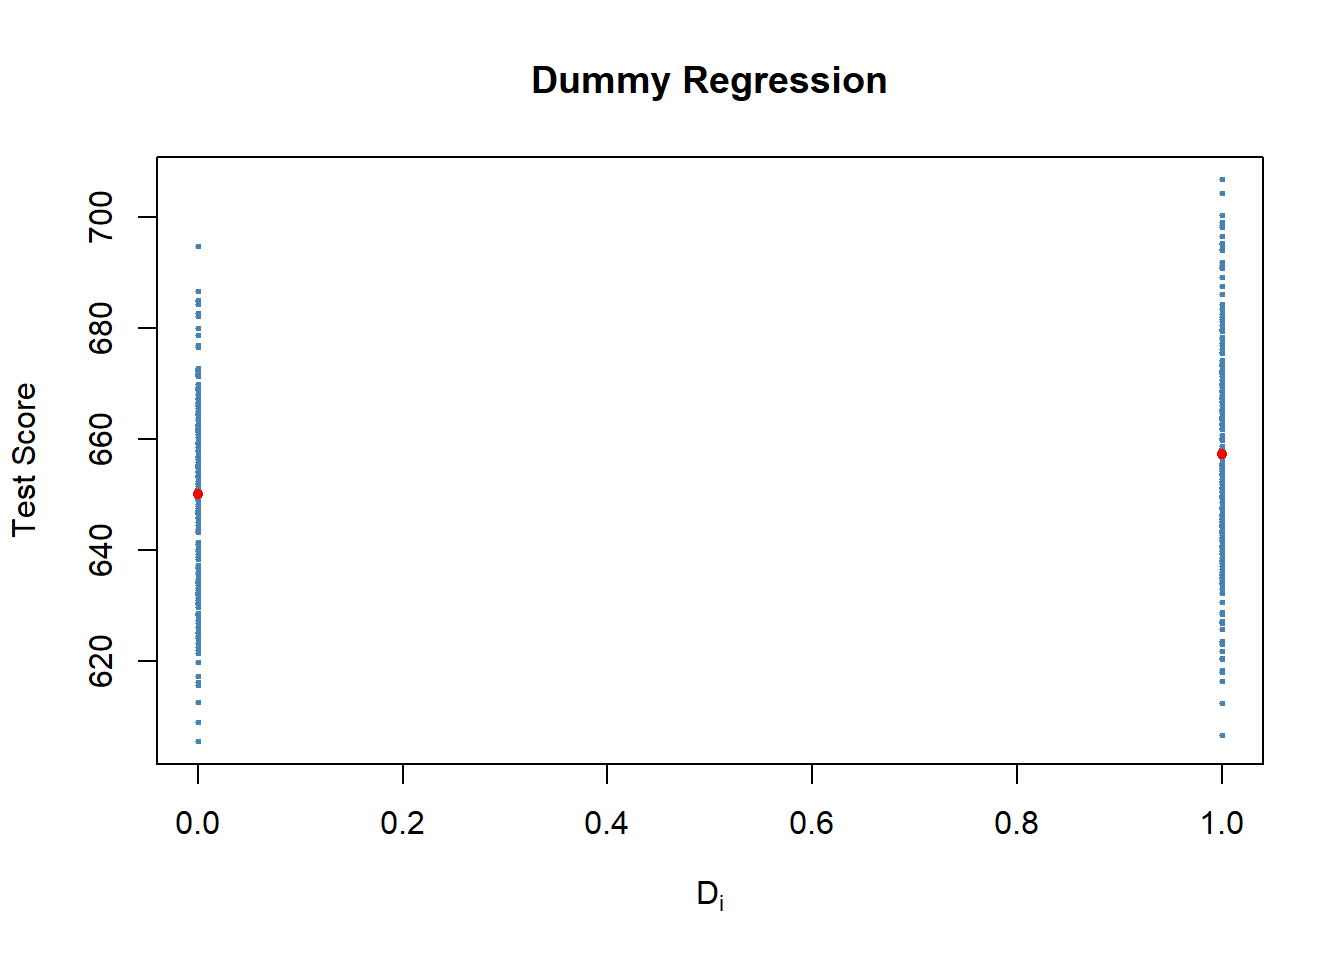
\includegraphics{URFITE_files/figure-latex/unnamed-chunk-108-1} \end{center}

We see that with \(D\) as the regressor, it is not useful to think of
\(\beta_1\) as a slope parameter since \(D_i \in \{0,1\}\), i.e.~we only
observe two discrete values instead of a continuoum of regressor values
lying (in some range) on the real line. Simply put, there is no
continuous line depicting the conditional expectation function
\(E(TestScore_i | D_i)\) since this function is solely defined for
\(X\)-positions \(0\) and \(1\).

Therefore, the interpretation of the coefficients in our regression
model is as follows:

\begin{itemize}
\item
  \(E(Y_i | D_i = 0) = \beta_0\) so \(\beta_0\) is the expected test
  score in districts where \(D_i=0\) i.e.~where \(STR\) is below \(20\).
\item
  \(E(Y_i | D_i = 1) = \beta_0 + \beta_1\) or, using the result above,
  \(\beta_1 = E(Y_i | D_i = 1) - E(Y_i | D_i = 0)\). Thus, \(\beta_1\)
  is the difference in group specific expectations, i.e.~the difference
  in expected test score between districts with \(STR < 20\) and those
  with \(STR \geq 20\).
\end{itemize}

We will now use R to estimate the dummy regression model as defined by
equations (5.2) - (5.3) .

\begin{Shaded}
\begin{Highlighting}[]
\CommentTok{# estimate the dummy regression model}
\NormalTok{dummy_model <-}\StringTok{ }\KeywordTok{lm}\NormalTok{(score }\OperatorTok{~}\StringTok{ }\NormalTok{D, }\DataTypeTok{data =}\NormalTok{ CASchools)}
\KeywordTok{summary}\NormalTok{(dummy_model)}
\end{Highlighting}
\end{Shaded}

\begin{verbatim}
## 
## Call:
## lm(formula = score ~ D, data = CASchools)
## 
## Residuals:
##     Min      1Q  Median      3Q     Max 
## -50.496 -14.029  -0.346  12.884  49.504 
## 
## Coefficients:
##             Estimate Std. Error t value Pr(>|t|)    
## (Intercept)  650.077      1.393 466.666  < 2e-16 ***
## D              7.169      1.847   3.882  0.00012 ***
## ---
## Signif. codes:  0 '***' 0.001 '**' 0.01 '*' 0.05 '.' 0.1 ' ' 1
## 
## Residual standard error: 18.74 on 418 degrees of freedom
## Multiple R-squared:  0.0348, Adjusted R-squared:  0.0325 
## F-statistic: 15.07 on 1 and 418 DF,  p-value: 0.0001202
\end{verbatim}

One can see that the expected test score in districts with \(STR < 20\)
(\(D_i = 1\)) is predicted to be \(650.1 + 7.17 = 657.27\) while
districs with \(STR \geq 20\) (\(D_i = 0\)) are expected to have an
average test score of only \(650.1\).

Group specific predictions can be added to the plot by execution of the
following code chunk:

\begin{Shaded}
\begin{Highlighting}[]
\CommentTok{# add group specific predictions to the plot}
\KeywordTok{points}\NormalTok{(}\DataTypeTok{x =}\NormalTok{ CASchools}\OperatorTok{$}\NormalTok{D, }
       \DataTypeTok{y =} \KeywordTok{predict}\NormalTok{(dummy_model), }
       \DataTypeTok{col =} \StringTok{"red"}\NormalTok{, }
       \DataTypeTok{pch =} \DecValTok{20}
\NormalTok{       )}
\end{Highlighting}
\end{Shaded}

Here we use the function \texttt{predict()} to obtain estimates of the
group specific means. The red dots represent these sample group
averages. Accordingly, \(\hat{\beta}_1 = 7.17\) can be seen as the
difference in group averages.

By inspection of the output generated with
\texttt{summary(dummy\_model)} we may also find an answer to the
question whether there is a statistically significant difference in
group means. This in turn would support the hypothesis that students
perform differently when they are taught in small classes rather than in
large groups. We can assess this by a two-tailed test of the hypothesis
\(H_0: \beta_1 = 0\). Conviniently the \(t\)-statistic and the
corresponding \(p\)-value for this test are computed defaultly by
\texttt{summary()}!

Since \texttt{t\ value} \(= 3.88 > 1.96\) we reject the null hypothesis
at the \(5\%\) level of significance. The same conclusion can be made
when using the \(p\)-value which reports significance to the
\(0.00012\%\) level.

As done with \texttt{linear\_model}, we may alternatively use the
\texttt{confint()} function to compute a \(95\%\) confidence interval
for the true difference in means and see if the hypothesised value is an
element of this confidence set.

\begin{Shaded}
\begin{Highlighting}[]
\CommentTok{# confidence intervals for coefficients in the dummy regression}
\KeywordTok{confint}\NormalTok{(dummy_model)}
\end{Highlighting}
\end{Shaded}

\begin{verbatim}
##                  2.5 %    97.5 %
## (Intercept) 647.338594 652.81500
## D             3.539562  10.79931
\end{verbatim}

We reject the hypothesis that there is no difference between group means
at the \(5\%\) significance level since \(\beta_{1,0} = 0\) lies outside
of \([3.54, 10.8]\), the \(95\%\) confidence interval for the
coefficient on \(D\).

\section{Heteroskedasticity and
Homoskedasticity}\label{heteroskedasticity-and-homoskedasticity}

All inference made in the previous chapters relies on the assumption
that the error variance does not vary as regressor values change. But
this will not necessarily be the case in most empirical applications.

Key Concept 5.4

Heteroskedasticity and Homoskedasticity

\begin{itemize}
\item
  We say that the error term of our regression model is homoskedastic if
  the variance of the conditional distribution of \(u_i\) given \(X_i\),
  \(Var(u_i|X_i=x)\), is constant \emph{for all} observations in our
  sample \[ \text{Var}(u_i|X_i=x) = \sigma^2 \ \forall \ i=1,\dots,n. \]
\item
  If instead there is dependence of the conditional variance of \(u_i\)
  on \(X_i\), the error term is said to be heteroskedastic. We then
  write
  \[ \text{Var}(u_i|X_i=x) = \sigma_i^2 \ \forall \ i=1,\dots,n. \]
\item
  Homoskedasticity is a \emph{special case} of heteroskedasticity.
\end{itemize}

For a better understanding of heteroskedasticity, we generate some
bivariate heteroskedastic data, estimate a linear regression model and
then use boxplots to depict the conditional distributions of the
residuals.

\begin{Shaded}
\begin{Highlighting}[]
\CommentTok{# load scales package for custom color opacities}
\KeywordTok{library}\NormalTok{(scales)}

\CommentTok{# Genrate some heteroskedastic data}
\KeywordTok{set.seed}\NormalTok{(}\DecValTok{123}\NormalTok{) }
\NormalTok{x <-}\StringTok{ }\KeywordTok{rep}\NormalTok{(}\KeywordTok{c}\NormalTok{(}\DecValTok{10}\NormalTok{,}\DecValTok{15}\NormalTok{,}\DecValTok{20}\NormalTok{,}\DecValTok{25}\NormalTok{),}\DataTypeTok{each=}\DecValTok{25}\NormalTok{)}
\NormalTok{e <-}\StringTok{ }\KeywordTok{rnorm}\NormalTok{(}\DecValTok{100}\NormalTok{, }\DataTypeTok{sd=}\DecValTok{12}\NormalTok{)                }
\NormalTok{i <-}\StringTok{ }\KeywordTok{order}\NormalTok{(}\KeywordTok{runif}\NormalTok{(}\DecValTok{100}\NormalTok{, }\DataTypeTok{max=}\KeywordTok{dnorm}\NormalTok{(e, }\DataTypeTok{sd=}\DecValTok{12}\NormalTok{))) }
\NormalTok{y <-}\StringTok{ }\DecValTok{720} \OperatorTok{-}\StringTok{ }\FloatTok{3.3} \OperatorTok{*}\StringTok{ }\NormalTok{x }\OperatorTok{+}\StringTok{ }\NormalTok{e[}\KeywordTok{rev}\NormalTok{(i)]}

\CommentTok{# Estimate the model }
\NormalTok{mod <-}\StringTok{ }\KeywordTok{lm}\NormalTok{(y }\OperatorTok{~}\StringTok{ }\NormalTok{x)}

\CommentTok{# Plot the data}
\KeywordTok{plot}\NormalTok{(}\DataTypeTok{x=}\NormalTok{x, }
     \DataTypeTok{y=}\NormalTok{y, }
     \DataTypeTok{main=}\StringTok{"An Example of Heteroskedasticity"}\NormalTok{,}
     \DataTypeTok{xlab =} \StringTok{"Student-Teacher Ratio"}\NormalTok{,}
     \DataTypeTok{ylab =} \StringTok{"Test Score"}\NormalTok{,}
     \DataTypeTok{cex =} \FloatTok{0.5}\NormalTok{, }
     \DataTypeTok{pch =} \DecValTok{19}\NormalTok{, }
     \DataTypeTok{xlim =} \KeywordTok{c}\NormalTok{(}\DecValTok{8}\NormalTok{,}\DecValTok{27}\NormalTok{), }
     \DataTypeTok{ylim =} \KeywordTok{c}\NormalTok{(}\DecValTok{600}\NormalTok{,}\DecValTok{710}\NormalTok{)}
\NormalTok{     )}

\CommentTok{# Add the regression line to the plot}
\KeywordTok{abline}\NormalTok{(mod, }\DataTypeTok{col=}\StringTok{"darkred"}\NormalTok{)}

\CommentTok{# Add boxplots to the plot}
\KeywordTok{boxplot}\NormalTok{(y }\OperatorTok{~}\StringTok{ }\NormalTok{x, }
        \DataTypeTok{add =} \OtherTok{TRUE}\NormalTok{, }
        \DataTypeTok{at =} \KeywordTok{c}\NormalTok{(}\DecValTok{10}\NormalTok{,}\DecValTok{15}\NormalTok{,}\DecValTok{20}\NormalTok{,}\DecValTok{25}\NormalTok{), }
        \DataTypeTok{col =} \KeywordTok{alpha}\NormalTok{(}\StringTok{"gray"}\NormalTok{, }\FloatTok{0.4}\NormalTok{), }
        \DataTypeTok{border =} \StringTok{"black"}
\NormalTok{        )}
\end{Highlighting}
\end{Shaded}

\begin{center}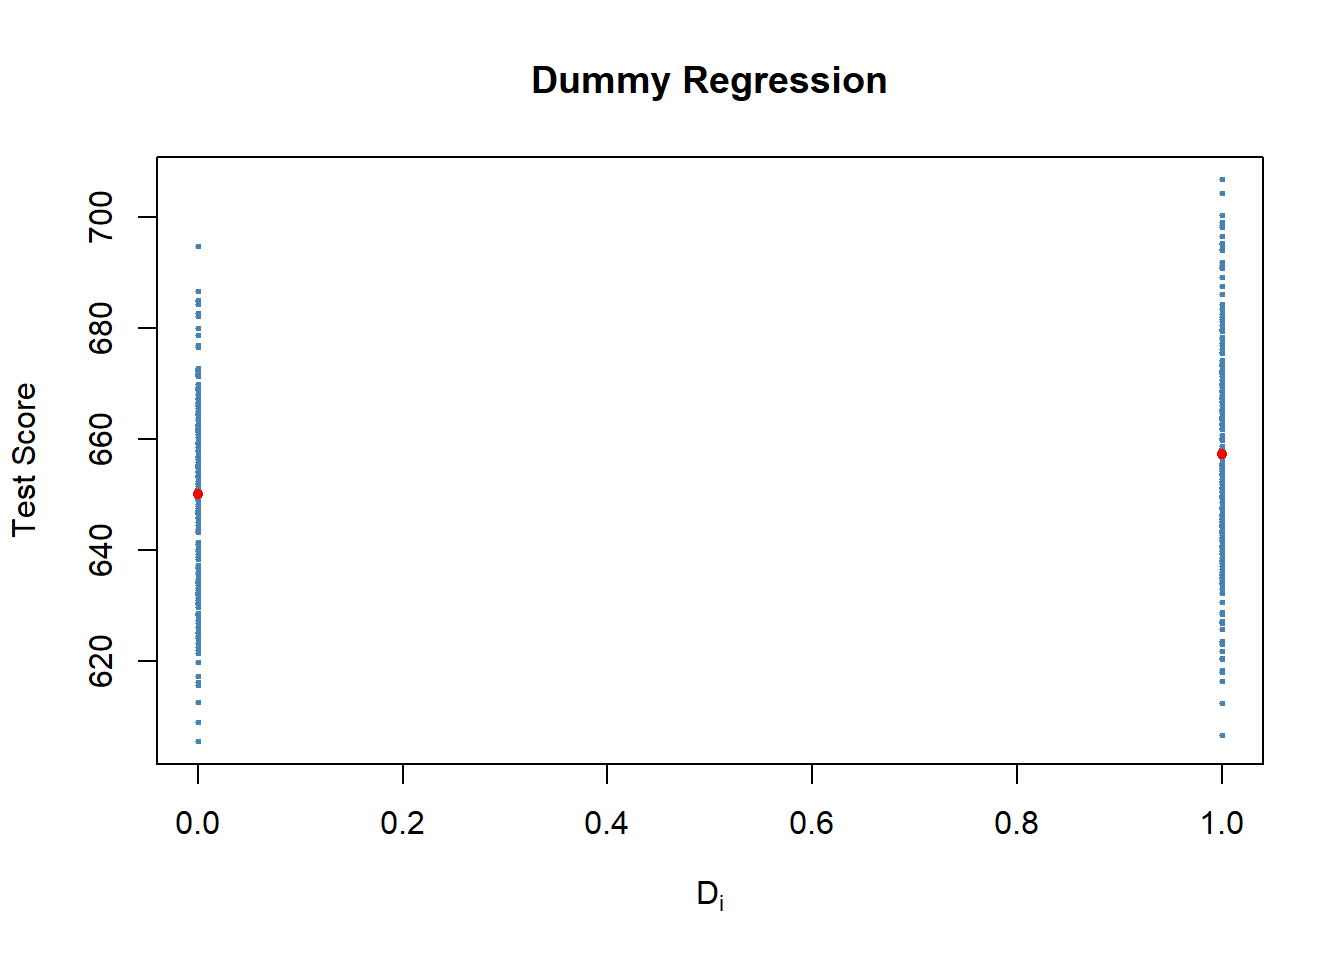
\includegraphics{URFITE_files/figure-latex/unnamed-chunk-112-1} \end{center}

For this artificial data it is straightforward to see that we face
unequal conditional error variances. Specifically, we observe that the
variance in test scores (and therefore the variance of the errors
committed) \emph{increases} with the student teacher ratio.

\subsection*{A Real-World Example for
Heteroskedasticity}\label{a-real-world-example-for-heteroskedasticity}
\addcontentsline{toc}{subsection}{A Real-World Example for
Heteroskedasticity}

Think about the economic value of education: if there would not be an
expected economic value-added to receiving education at university, You
probably would not be reading this script right now. A starting point to
empirical verification of such a relation exists is to have data on
individuals that are in an employment relationship. More precisely, we
need data on wages and education in order to work with a model like

\[ wage_i = \beta_0 + \beta_1 \cdot education_i + u_i. \]

What can be presumed about this relation? It is likely that, on average,
higher educated workers earn more money than workers with less education
so we expect to estimate an upward sloping regression line. Also it
seems plausible that workers with better education are more likely to
meet the requirements for the well-paid jobs. However, workers with low
education will have no shot at those well-paid jobs. Therefore it seems
plausible that the distribution of earnings spreads out as education
increases. In other words: we expect that there is heteroskedasticity!

To verify this empirically we may use real data on hourly earnings and
the number of years of education of employees. Such data can be found in
\texttt{CPSSWEducation}. This data set is part of the package
\texttt{AER} and stems from the Current Population Survey (CPS) which is
conducted periodically by the \href{http://www.bls.gov/}{Bureau of Labor
Statistics} in the US.

The subsequent code chunks demonstrate how to load the data into R and
how to produce a plot in the fashion of figure 5.3 in the book.

\begin{Shaded}
\begin{Highlighting}[]
\CommentTok{# load package and attach data}
\KeywordTok{library}\NormalTok{(AER)}
\KeywordTok{data}\NormalTok{(}\StringTok{"CPSSWEducation"}\NormalTok{)}
\KeywordTok{attach}\NormalTok{(CPSSWEducation)}
\end{Highlighting}
\end{Shaded}

\begin{verbatim}
## The following objects are masked from CPSSWEducation (pos = 9):
## 
##     age, earnings, education, gender
\end{verbatim}

\begin{Shaded}
\begin{Highlighting}[]
\CommentTok{# get an overview}
\KeywordTok{summary}\NormalTok{(CPSSWEducation)}
\end{Highlighting}
\end{Shaded}

\begin{verbatim}
##       age          gender        earnings        education    
##  Min.   :29.0   female:1202   Min.   : 2.137   Min.   : 6.00  
##  1st Qu.:29.0   male  :1748   1st Qu.:10.577   1st Qu.:12.00  
##  Median :29.0                 Median :14.615   Median :13.00  
##  Mean   :29.5                 Mean   :16.743   Mean   :13.55  
##  3rd Qu.:30.0                 3rd Qu.:20.192   3rd Qu.:16.00  
##  Max.   :30.0                 Max.   :97.500   Max.   :18.00
\end{verbatim}

\begin{Shaded}
\begin{Highlighting}[]
\CommentTok{# estimate a simple regression model}
\NormalTok{labor_model <-}\StringTok{ }\KeywordTok{lm}\NormalTok{(earnings }\OperatorTok{~}\StringTok{ }\NormalTok{education)}

\CommentTok{# plot observations and add the regression line}
\KeywordTok{plot}\NormalTok{(education, }
\NormalTok{     earnings, }
     \DataTypeTok{ylim =} \KeywordTok{c}\NormalTok{(}\DecValTok{0}\NormalTok{,}\DecValTok{150}\NormalTok{)}
\NormalTok{     )}

\KeywordTok{abline}\NormalTok{(labor_model, }\DataTypeTok{col=}\StringTok{"steelblue"}\NormalTok{, }\DataTypeTok{lwd=}\DecValTok{2}\NormalTok{)}
\end{Highlighting}
\end{Shaded}

\begin{center}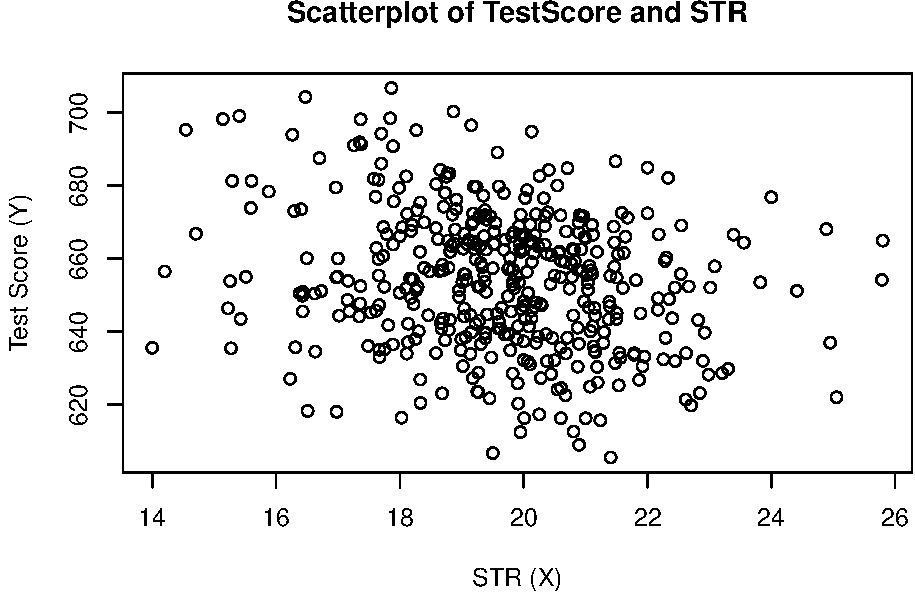
\includegraphics{URFITE_files/figure-latex/unnamed-chunk-113-1} \end{center}

From inspecting the plot we can tell that the mean of the distribution
of earnings increases with the level of education. This is also
suggested by formal analysis: the estimated regression model stored in
\texttt{labor\_mod} asserts that there is a positive relation between
years of education and earnings.

\begin{Shaded}
\begin{Highlighting}[]
\NormalTok{labor_model}
\end{Highlighting}
\end{Shaded}

\begin{verbatim}
## 
## Call:
## lm(formula = earnings ~ education)
## 
## Coefficients:
## (Intercept)    education  
##      -3.134        1.467
\end{verbatim}

The estimated regression equation states that, on average, an additional
year of education increases a workers hourly earnings by about
\(\$ 1.47\). Once more we use \texttt{confint()} to obtain a \(95\%\)
confidence interval for both regression coefficients.

\begin{Shaded}
\begin{Highlighting}[]
\KeywordTok{confint}\NormalTok{(labor_model)}
\end{Highlighting}
\end{Shaded}

\begin{verbatim}
##                 2.5 %    97.5 %
## (Intercept) -5.015248 -1.253495
## education    1.330098  1.603753
\end{verbatim}

Since the intervall is \([1.33, 1.60]\) we can reject the hypothesis
that the coefficient on \texttt{education} is zero at the \(5\%\) level.

What is more, the plot indicates that there is heteroskedasticity: if we
assume the regression line to be a reasonably good representation of the
conditional mean function \(E(earnings_i\vert education_i)\), the
dispersion of hourly earnings around that function cleary increases with
the level of education, i.e.~the variance of the distribution of
earnings increases. In other words: the variance of the residuals
increases with the years of education so that the regression errors are
heteroskedastic. This example makes a case that it is doubtful to assume
homoskedasticity in many economic applications.

\subsection*{Should We Care About
Heteroskedasticity?}\label{should-we-care-about-heteroskedasticity}
\addcontentsline{toc}{subsection}{Should We Care About
Heteroskedasticity?}

To answer this question, let us see how the variance of \(\hat\beta_1\)
is computed under the assumption of homoskedasticity. In this case we
have

\[ \sigma^2_{\hat\beta_1} = \frac{\sigma^2_u}{n \cdot \sigma^2_X} \tag{5.5} \]

which is a simplified version of the general equation (4.1) presented in
Key Concept 4.4. See Appendix 5.1 of the book for details on the
derivation. The \texttt{summary()} function in R estimates (5.5) by

\[ \overset{\sim}{\sigma}^2_{\hat\beta_1} = \frac{SER^2}{\sum_{i=1}^n (X_i - \overline{X})^2} \ \ \text{where} \ \ SER=\frac{1}{n-2} \sum_{i=1}^n \hat u_i^2. \]

Thus \texttt{summary()} estimates the \emph{homoskedasticity-only}
standard error

\[ \sqrt{ \overset{\sim}{\sigma}^2_{\hat\beta_1} } = \sqrt{ \frac{SER^2}{\sum(X_i - \overline{X})^2} }. \]

This in fact is an estimator for the standard deviation of the estimator
\(\hat{\beta}_1\) that is \emph{inconsistent} for the true value
\(\sigma^2_{\hat\beta_1}\) when there is heteroskedasticity. The
implication is that \(t\)-statistics computed in the manner of Key
Concept 5.1 do not have a standard normal distribution, even in large
samples. This issue may invalidate inference drawn when using the
previously treated tools for hypothesis testing: we should be cautious
when making statements about the significance of regression coefficients
on the basis of \(t\)-statistics as computed by \texttt{summary()} or
confidence intervals produced by \texttt{confint()} if it is doubtful
for the assumption of homoskedasticity to hold!

We will now use R to compute the homoskedasticity-only standard error
estimate for \(\hat{\beta}_1\) in the test score regression model
\texttt{linear\_model} by hand and see if it matches the value produced
by \texttt{summary()}.

\begin{Shaded}
\begin{Highlighting}[]
\CommentTok{# Store model summary in 'mod'}
\NormalTok{model <-}\StringTok{ }\KeywordTok{summary}\NormalTok{(linear_model)}

\CommentTok{# Extract the standard error of the regression from model summary}
\NormalTok{SER <-}\StringTok{ }\NormalTok{model}\OperatorTok{$}\NormalTok{sigma}

\CommentTok{# Compute the variation in 'size'}
\NormalTok{V <-}\StringTok{ }\NormalTok{(}\KeywordTok{nrow}\NormalTok{(CASchools)}\OperatorTok{-}\DecValTok{1}\NormalTok{) }\OperatorTok{*}\StringTok{ }\KeywordTok{var}\NormalTok{(CASchools}\OperatorTok{$}\NormalTok{STR)}

\CommentTok{# Compute the standard error of the slope parameter's estimator and print it}
\NormalTok{SE.beta_}\FloatTok{1.}\NormalTok{hat <-}\StringTok{ }\KeywordTok{sqrt}\NormalTok{(SER}\OperatorTok{^}\DecValTok{2}\OperatorTok{/}\NormalTok{V)}
\NormalTok{SE.beta_}\FloatTok{1.}\NormalTok{hat}
\end{Highlighting}
\end{Shaded}

\begin{verbatim}
## [1] 0.4798255
\end{verbatim}

\begin{Shaded}
\begin{Highlighting}[]
\CommentTok{# Use logical operators to see if the value computed by hand matches the one provided # in mod$coefficients. Round estimates to four decimal places}

\KeywordTok{round}\NormalTok{(model}\OperatorTok{$}\NormalTok{coefficients[}\DecValTok{2}\NormalTok{,}\DecValTok{2}\NormalTok{], }\DecValTok{4}\NormalTok{) }\OperatorTok{==}\StringTok{ }\KeywordTok{round}\NormalTok{(SE.beta_}\FloatTok{1.}\NormalTok{hat, }\DecValTok{4}\NormalTok{)}
\end{Highlighting}
\end{Shaded}

\begin{verbatim}
## [1] TRUE
\end{verbatim}

Indeed, the estimated values are equal.

\subsection*{Computation of Heteroskedasticity-Robust Standard
Errors}\label{computation-of-heteroskedasticity-robust-standard-errors}
\addcontentsline{toc}{subsection}{Computation of
Heteroskedasticity-Robust Standard Errors}

Cosistent estimation of \(\sigma_{\hat{\beta}_1}\) under
heteroskedasticity is granted when the following \emph{robust} estimator
is used.

\[ SE(\hat{\beta}_1) = \sqrt{ \frac{ \frac{1}{n-2} \sum_{i=1}^n (X_i - \overline{X})^2 \hat{u}_i^2 }{ \left[ \frac{1}{n} \sum_{i=1}^n (X_i - \overline{X})^2  \right]^2} } \tag{5.6} \]

Standard error estimates computed this way are also referred to as
\href{https://en.wikipedia.org/wiki/Heteroscedasticity-consistent_standard_errors}{Eicker-Huber-White
standard errors}. It can be quite cumbersome to do this calculation by
hand. Luckily, there are R function for that purpose. A convenient one,
named \texttt{vcovHC()} is part of the \texttt{sandwich} package. This
function can compute a variety of standard error estimators. The one
brought forward in (5.6) is computed when the argument \texttt{type} is
set to \texttt{"HC0"}.

Let us now compute robust standard error estimates for the coefficients
in \texttt{linear\_model}.

\begin{Shaded}
\begin{Highlighting}[]
\CommentTok{# load the sandwich package}
\KeywordTok{library}\NormalTok{(sandwich)}

\CommentTok{# compute robust standard error estimates}
\NormalTok{vcov <-}\StringTok{ }\KeywordTok{vcovHC}\NormalTok{(linear_model, }\DataTypeTok{type =} \StringTok{"HC0"}\NormalTok{)}
\NormalTok{vcov}
\end{Highlighting}
\end{Shaded}

\begin{verbatim}
##             (Intercept)        STR
## (Intercept)  106.908469 -5.3383689
## STR           -5.338369  0.2685841
\end{verbatim}

The output of \texttt{vcovHC()} is the variance-covariance matrix of
coefficient estimates. We are interested in the square root of the
diagonal elements of this matrix since these values are the standard
error estimates we seek.

\BeginKnitrBlock{rmdknit}
When we have k \textgreater{} 1 regressors, writing down the equations
for a regression model becomes very messy. A more convinient way to
denote and estimate so-called multiple regression models is matrix
algebra. This is why functions like vcovHC() produce matrices. In the
simple linear regression model, the variances and covariances of the
coefficient estimators can be gathered in the variance-covariance matrix

\begin{equation}
\text{Var}
  \begin{pmatrix}
    \hat\beta_0 \\
    \hat\beta_1
  \end{pmatrix} = 
\begin{pmatrix}
  \text{Var}(\hat\beta_0) & \text{Cov}(\hat\beta_0,\hat\beta_1) \\
\text{Cov}(\hat\beta_0,\hat\beta_1) & \text{Var}(\hat\beta_1)
\end{pmatrix}
\end{equation}

which is a symmetric matrix. So vcovHC() gives us
\(\widehat{\text{Var}}(\hat\beta_0)\),
\(\widehat{\text{Var}}(\hat\beta_1)\) and
\(\widehat{\text{Cov}}(\hat\beta_0,\hat\beta_1)\) but most of the time
we are interested in the diagonal elements of the estimated matrix.
\EndKnitrBlock{rmdknit}

\begin{Shaded}
\begin{Highlighting}[]
\CommentTok{# compute the square root of the diagonal elements in vcov}
\NormalTok{robust_se <-}\StringTok{ }\KeywordTok{sqrt}\NormalTok{(}\KeywordTok{diag}\NormalTok{(vcov))}
\NormalTok{robust_se}
\end{Highlighting}
\end{Shaded}

\begin{verbatim}
## (Intercept)         STR 
##   10.339655    0.518251
\end{verbatim}

Now assume we want to generate a coefficient summary as provided by
\texttt{summary()} but with \emph{robust} standard error estimates for
the coefficient estimators, robust \(t\)-statistics and corresponding
\(p\)-values for the regression model \texttt{linear\_model}. This can
be done using \texttt{coeftest()} from the package \texttt{lmtest}, see
\texttt{?coeftest}. Further we specify in the argument \texttt{vcov.}
that \texttt{vcov}, the Eicker-Huber-White estimate of the variance
matrix we have computed before should be used.

\begin{Shaded}
\begin{Highlighting}[]
\CommentTok{# We invoke the function `coeftest()` on our model}
\KeywordTok{coeftest}\NormalTok{(linear_model, }\DataTypeTok{vcov. =}\NormalTok{ vcov)}
\end{Highlighting}
\end{Shaded}

\begin{verbatim}
## 
## t test of coefficients:
## 
##              Estimate Std. Error t value  Pr(>|t|)    
## (Intercept) 698.93295   10.33966  67.597 < 2.2e-16 ***
## STR          -2.27981    0.51825  -4.399 1.382e-05 ***
## ---
## Signif. codes:  0 '***' 0.001 '**' 0.01 '*' 0.05 '.' 0.1 ' ' 1
\end{verbatim}

We see that values reported in the column \texttt{Std.\ Error} equal the
ones received using \texttt{sqrt(diag(vcov))}.

How severe are the implications of using homoskedasticity-only standard
errors in the presence of heteroskedasticity? The answer is: it depends.
As mentioned above we may face the risk of drawing wrong conclusions
when conducting significance tests. Let us illustrate this by generating
another example of a heteroskedastic data set and use it to estimate a
simple regression model. We take

\[ Y_i = \beta_1 \cdot X_i + u_i \ \ , \ \ u_i \overset{i.i.d.}{\sim} N(0,0.36 \cdot X_i^2)  \]

with \(\beta_1=1\) as the data generating process. The assumption of
homoskedasticity is violated since the variance of the errors is a
non-linear increasing function of \(X_i\) but the errors have zero mean
and are i.i.d. such that the assumptions made in Key Concept 4.3 are not
violated. As before, the true conditional mean function we are
interested in estimating is

\[ E(Y_i\vert X_i) = X_i. \]

\begin{Shaded}
\begin{Highlighting}[]
\CommentTok{# set random seed}
\KeywordTok{set.seed}\NormalTok{(}\DecValTok{21}\NormalTok{)}

\CommentTok{# generate heteroskedastic data }
\NormalTok{X <-}\StringTok{ }\DecValTok{1}\OperatorTok{:}\DecValTok{1000}
\NormalTok{Y <-}\StringTok{ }\KeywordTok{rnorm}\NormalTok{(}\DataTypeTok{n =} \DecValTok{1000}\NormalTok{, }\DataTypeTok{mean =}\NormalTok{ X, }\DataTypeTok{sd =} \FloatTok{0.6}\OperatorTok{*}\NormalTok{X)}

\CommentTok{# estimate a simple regression model}
\NormalTok{reg <-}\StringTok{ }\KeywordTok{lm}\NormalTok{(Y }\OperatorTok{~}\StringTok{ }\NormalTok{X)}
\end{Highlighting}
\end{Shaded}

We plot the data and add the regression line.

\begin{Shaded}
\begin{Highlighting}[]
\CommentTok{# plot the data}
\KeywordTok{plot}\NormalTok{(X, Y, }\DataTypeTok{pch =} \DecValTok{19}\NormalTok{, }\DataTypeTok{col=}\StringTok{"steelblue"}\NormalTok{, }\DataTypeTok{cex =} \FloatTok{0.8}\NormalTok{)}

\CommentTok{# add the regression line to the plot}
\KeywordTok{abline}\NormalTok{(reg, }\DataTypeTok{col =} \StringTok{"darkred"}\NormalTok{, }\DataTypeTok{lwd =} \FloatTok{1.5}\NormalTok{)}
\end{Highlighting}
\end{Shaded}

\begin{center}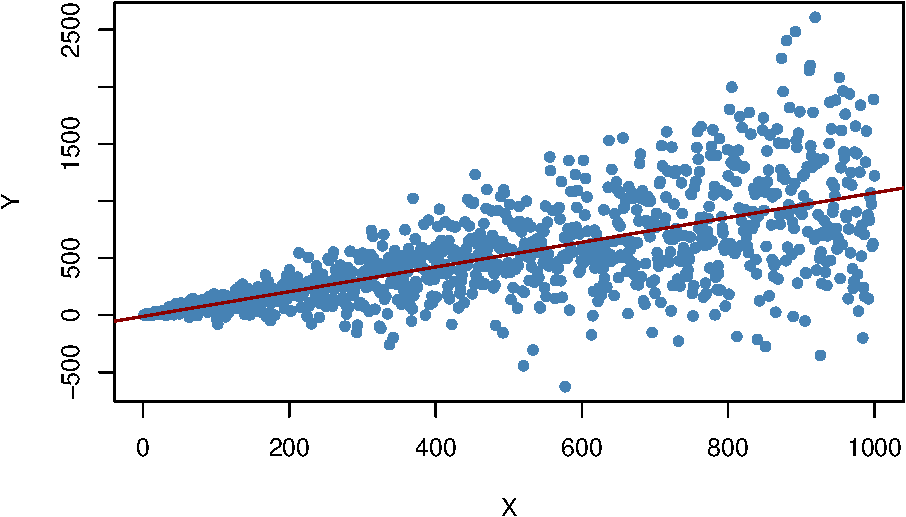
\includegraphics{URFITE_files/figure-latex/unnamed-chunk-121-1} \end{center}

The plot clearly shows that the data are heteroskedastic as the variance
of \(Y\) grows with \(X\). We continue by conducting a significance test
of the (true) null hypothesis \(H_0: \beta_1 = 1\) twice, once using the
homoskedasticity-only standard error formula and once with the robust
version (5.6). An idiomatic way to do this in R is the function
\texttt{linearHypothesis()} from the package \texttt{car}, see
\texttt{?linearHypothesis}. It allows to test linear hypotheses about
parameters in linear models in a similar way as done with a
\(t\)-statistic and offers various robust covariance matrix estimators.
We test by comparing the tests' \(p\)-values to the significance level
of \(5\%\).

\BeginKnitrBlock{rmdknit}
linearHypothesis() computes a test statistic that follows an \(F\)
distribution under the null hypothesis. We will not loose too much words
on the theory behind it at this time. In general, the core idea of the
\(F\) test is to compare the fit of different models. When testing a
hypothesis about a \emph{single} coefficient using a \(F\) test, one can
show that the test statistic is simply the square of the corresponding
\(t\)-statistic:

\[ F = t^2 = \frac{\hat\beta_i - \beta_{i,0}}{SE(\hat\beta_i)} \sim F_{1,n-k-1}  \]

In linearHypothesis(), the hypothesis must be provided as a
\emph{string}. The function returns an object of class anova which
contains further information on the test that can be accessed using the
\$ operator. For example, we can obtain the test's \(p\)-value by adding
\$`Pr(\textgreater{}F)' right behind the function call.
\EndKnitrBlock{rmdknit}

\begin{Shaded}
\begin{Highlighting}[]
\CommentTok{# test using default standard error}
\KeywordTok{linearHypothesis}\NormalTok{(reg, }\DataTypeTok{hypothesis.matrix =} \StringTok{"X = 1"}\NormalTok{)}\OperatorTok{$}\StringTok{'Pr(>F)'}\NormalTok{[}\DecValTok{2}\NormalTok{] }\OperatorTok{<}\StringTok{ }\FloatTok{0.05}
\end{Highlighting}
\end{Shaded}

\begin{verbatim}
## [1] TRUE
\end{verbatim}

\begin{Shaded}
\begin{Highlighting}[]
\CommentTok{# test using robust standard error}
\KeywordTok{linearHypothesis}\NormalTok{(reg, }\DataTypeTok{hypothesis.matrix =} \StringTok{"X = 1"}\NormalTok{, }\DataTypeTok{white.adjust =} \StringTok{"hc0"}\NormalTok{)}\OperatorTok{$}\StringTok{'Pr(>F)'}\NormalTok{[}\DecValTok{2}\NormalTok{] }\OperatorTok{<}\StringTok{ }\FloatTok{0.05}
\end{Highlighting}
\end{Shaded}

\begin{verbatim}
## [1] FALSE
\end{verbatim}

This is a good example of what can go wrong if we do not care for
heteroskedasticity: for the data set at hand the default method rejects
the null hypothesis \(\beta_1 = 1\) although it is true. Using the
robust standard error though the test does not reject the null. Of
course we could argue that this is just a coincidence and both tests are
equally well in maintaining the type I error rate of \(5\%\). This can
be further investigated by computing Monte Carlo estimates of the
rejection frequencies of both tests on the basis of a large number of
random samples. We proceed as follows:

\begin{itemize}
\tightlist
\item
  initialize vectors \texttt{t} and \texttt{t.rob} as type
  \texttt{numeric} with length \(10000\).
\item
  Using a \texttt{for()} loop, we generate \(10000\) heteroskedastic
  random samples of size \(1000\), estimate the regression model and
  check whether the tests wrongly reject the null at the level of
  \(5\%\) using comparison operators. The results are stored in the
  respective vectors \texttt{t} and \texttt{t.rob}.
\item
  After the simulation, we compute the fraction of rejections for both
  tests.
\end{itemize}

\begin{Shaded}
\begin{Highlighting}[]
\CommentTok{# initialize vectors t and t.rob}
\NormalTok{t <-}\StringTok{ }\KeywordTok{numeric}\NormalTok{(}\DecValTok{10000}\NormalTok{)}
\NormalTok{t.rob <-}\StringTok{ }\KeywordTok{numeric}\NormalTok{(}\DecValTok{10000}\NormalTok{)}

\CommentTok{# loop sampling and estimation}
\ControlFlowTok{for}\NormalTok{ (i }\ControlFlowTok{in} \DecValTok{1}\OperatorTok{:}\DecValTok{10000}\NormalTok{) \{}
  
  \CommentTok{# sample data}
\NormalTok{  X <-}\StringTok{ }\DecValTok{1}\OperatorTok{:}\DecValTok{1000}
\NormalTok{  Y <-}\StringTok{ }\KeywordTok{rnorm}\NormalTok{(}\DataTypeTok{n =} \DecValTok{1000}\NormalTok{, }\DataTypeTok{mean =}\NormalTok{ X, }\DataTypeTok{sd =} \FloatTok{0.6}\OperatorTok{*}\NormalTok{X)}

  \CommentTok{# estimate regression model}
\NormalTok{  reg <-}\StringTok{ }\KeywordTok{lm}\NormalTok{(Y }\OperatorTok{~}\StringTok{ }\NormalTok{X)}

  \CommentTok{# homoskedasdicity-only significance test}
\NormalTok{  t[i] <-}\StringTok{ }\KeywordTok{linearHypothesis}\NormalTok{(reg, }\StringTok{"X = 1"}\NormalTok{)}\OperatorTok{$}\StringTok{'Pr(>F)'}\NormalTok{[}\DecValTok{2}\NormalTok{] }\OperatorTok{<}\StringTok{ }\FloatTok{0.05}

  \CommentTok{# robust significance test}
\NormalTok{  t.rob[i] <-}\StringTok{ }\KeywordTok{linearHypothesis}\NormalTok{(reg, }\StringTok{"X = 1"}\NormalTok{, }\DataTypeTok{white.adjust =} \StringTok{"hc0"}\NormalTok{)}\OperatorTok{$}\StringTok{'Pr(>F)'}\NormalTok{[}\DecValTok{2}\NormalTok{] }\OperatorTok{<}\StringTok{ }\FloatTok{0.05}

\NormalTok{\}}

\CommentTok{# compute fraction of rejections}
\KeywordTok{cbind}\NormalTok{(}\DataTypeTok{t =} \KeywordTok{sum}\NormalTok{(t), }\DataTypeTok{t.rob =} \KeywordTok{sum}\NormalTok{(t.rob)) }\OperatorTok{/}\StringTok{ }\DecValTok{10000}
\end{Highlighting}
\end{Shaded}

\begin{verbatim}
##           t  t.rob
## [1,] 0.0762 0.0524
\end{verbatim}

The results show that we face an increased risk of falsely rejecting the
null using the homoskedasticity-only standard error for the testing
problem at hand: with the common standard error estimator, \(7.62\%\) of
all tests reject the null hypothesis falsely. In contrast, with the
robust test statistic we are close to the nominal level of \(5\%\).

\section{The Gauss-Markov Theorem}\label{the-gauss-markov-theorem}

When estimating regression models, we know that the results of the
estimation procedure are outcomes of a random process. However, when
using unbiased estimators, at least on average, we estimate the true
parameter. When comparing different unbiased estimators, it is therefore
interesting to know which one has the highest precision: being aware
that the likelihood of estimating the \emph{exact} value of the
parameter of interest is \(0\) in an empirical application, we want to
make sure that the likelihood of obtaining an estimate very close to the
true value is as high as possible. We want to use the estimator with the
lowest variance of all unbiased estimators. The Gauss-Markov theorem
states that the OLS estimator has this property under certain
conditions.

Key Concept 5.5

The Gauss-Markov Theorem for \(\hat{\beta}_1\)

Suppose that the assumptions made in Key Concept 4.3 hold \emph{and}
that the errors are \emph{homoskedastic}. The OLS estimator is the best
(in the sense of smallest variance) linear conditionally unbiased
estimator (BLUE) in this setting.

Let us have a closer look at what this means:

\begin{itemize}
\item
  Estimators of \(\beta_1\) that are linear functions of the
  \(Y_1, \dots, Y_n\) and that are unbiased conditionally on the
  regressor \(X_1, \dots, X_n\) can be written as
  \[ \overset{\sim}{\beta}_1 = \sum_{i=1}^n a_i Y_i \] where the \(a_i\)
  are weights that are allowed to depend on the \(X_i\) but \emph{not}
  on the \(Y_i\).
\item
  We already know that \(\overset{\sim}{\beta}_1\) has a sampling
  distribution: \(\overset{\sim}{\beta}_1\) is a linear function of the
  \(Y_i\) which are random variables. If now
  \[ E(\overset{\sim}{\beta}_1 | X_1, \dots, X_n) = \beta_1 \] we say
  that \(\overset{\sim}{\beta}_1\) is a linear unbiased estimator of
  \(\beta_1\), conditionally on the \(X_1, \dots, X_n\).
\item
  We may ask if \(\overset{\sim}{\beta}_1\) is also the \emph{best}
  estimator in this class, i.e.~the most efficient one of all linear
  unbiased estimators where ``most efficient'' means smallest variance.
  The weights \(a_i\) play an important role here and it turns out that
  OLS uses just the right weights to have the BLUE property.
\end{itemize}

\subsection*{R Simulation Study: BLUE
Estimator}\label{r-simulation-study-blue-estimator}
\addcontentsline{toc}{subsection}{R Simulation Study: BLUE Estimator}

Consider the case of a regression of \(Y_i,\dots,Y_n\) only on a
constant. Here, the \(Y_i\) are assumed to be a random sample from a
population with mean \(\mu\) and variance \(\sigma^2\). We know that the
OLS estimator in this model is simply the sample mean:

\begin{equation}
\hat{\beta}_1 = \overline{\beta}_1 = \sum_{i=1}^n \underbrace{\frac{1}{n}}_{=a_i} Y_i \label{eq:bluemean}
\end{equation}

Clearly, each observation is weighted by

\[a_i = \frac{1}{n}.\]

and We also know that
\(\text{Var}(\hat{\beta}_1)=\text{Var}(\hat\beta_1)=\frac{\sigma^2}{n}\).

We will now use R for a simulation study that illustrates what happens
to the variance of \eqref{eq:bluemean} if different weights
\[ w_i = \frac{1 \pm \epsilon}{n} \] are assigned to either half of the
sample \(Y_1, \dots, Y_n\) instead of using \(\frac{1}{n}\), the weights
implied by OLS.

\begin{Shaded}
\begin{Highlighting}[]
\CommentTok{# Set sample size and number of repititions}
\NormalTok{n <-}\StringTok{ }\DecValTok{100}      
\NormalTok{reps <-}\StringTok{ }\FloatTok{1e5}

\CommentTok{# Choose epsilon and create a vector of weights as defined above}
\NormalTok{epsilon <-}\StringTok{ }\FloatTok{0.8}
\NormalTok{w <-}\StringTok{ }\KeywordTok{c}\NormalTok{(}\KeywordTok{rep}\NormalTok{((}\DecValTok{1}\OperatorTok{+}\NormalTok{epsilon)}\OperatorTok{/}\NormalTok{n,n}\OperatorTok{/}\DecValTok{2}\NormalTok{), }
       \KeywordTok{rep}\NormalTok{((}\DecValTok{1}\OperatorTok{-}\NormalTok{epsilon)}\OperatorTok{/}\NormalTok{n,n}\OperatorTok{/}\DecValTok{2}\NormalTok{) }
\NormalTok{      )}

\CommentTok{# Draw a random sample y_1,...,y_n from the standard normal distribution, }
\CommentTok{# use both estimators 1e5 times and store the result in thr vectors ols and }
\CommentTok{# weightedestimator}

\NormalTok{ols <-}\StringTok{ }\KeywordTok{rep}\NormalTok{(}\OtherTok{NA}\NormalTok{, reps)}
\NormalTok{weightedestimator <-}\StringTok{ }\KeywordTok{rep}\NormalTok{(}\OtherTok{NA}\NormalTok{, reps)}

\ControlFlowTok{for}\NormalTok{ (i }\ControlFlowTok{in} \DecValTok{1}\OperatorTok{:}\NormalTok{reps) \{}
\NormalTok{  y <-}\StringTok{ }\KeywordTok{rnorm}\NormalTok{(n)}
\NormalTok{  ols[i] <-}\StringTok{ }\KeywordTok{mean}\NormalTok{(y)}
\NormalTok{  weightedestimator[i] <-}\StringTok{ }\KeywordTok{crossprod}\NormalTok{(w,y)}
\NormalTok{\}}

\CommentTok{# Plot kernel density estimates of the estimators' distributions }

\NormalTok{## OLS}
\KeywordTok{plot}\NormalTok{(}\KeywordTok{density}\NormalTok{(ols), }
     \DataTypeTok{col =} \StringTok{"purple"}\NormalTok{, }
     \DataTypeTok{lwd =} \DecValTok{3}\NormalTok{, }
     \DataTypeTok{main =} \StringTok{"Density of OLS and Weighted Estimator"}\NormalTok{,}
     \DataTypeTok{xlab =} \StringTok{"Estimates"}
\NormalTok{     )}

\NormalTok{## Weighted}
\KeywordTok{lines}\NormalTok{(}\KeywordTok{density}\NormalTok{(weightedestimator), }
      \DataTypeTok{col =} \StringTok{"steelblue"}\NormalTok{, }
      \DataTypeTok{lwd =} \DecValTok{3}
\NormalTok{      ) }

\NormalTok{## Add a dashed line at 0 and a legend to the plot}
\KeywordTok{abline}\NormalTok{(}\DataTypeTok{v =} \DecValTok{0}\NormalTok{, }\DataTypeTok{lty =} \DecValTok{2}\NormalTok{)}
\KeywordTok{legend}\NormalTok{(}\StringTok{'topright'}\NormalTok{, }
       \KeywordTok{c}\NormalTok{(}\StringTok{"OLS"}\NormalTok{,}\StringTok{"Weighted"}\NormalTok{), }
       \DataTypeTok{col =} \KeywordTok{c}\NormalTok{(}\StringTok{"purple"}\NormalTok{,}\StringTok{"steelblue"}\NormalTok{), }
       \DataTypeTok{lwd =} \DecValTok{3}
\NormalTok{       )}
\end{Highlighting}
\end{Shaded}

\begin{center}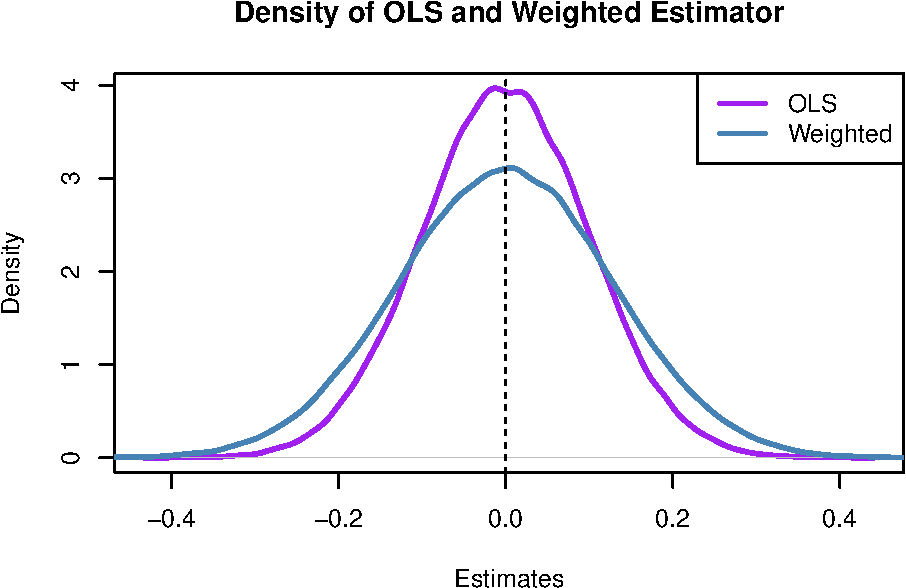
\includegraphics{URFITE_files/figure-latex/unnamed-chunk-124-1} \end{center}

What conclusion can we draw from the result?

\begin{itemize}
\tightlist
\item
  Both estimators seem to be unbiased: the means of their estimated
  distributions are zero.
\item
  The \texttt{weightedestimator} is less efficient than the \texttt{ols}
  estimator: there is higher dispersion when weights are
  \(w_i = \frac{1 \pm 0.8}{100}\) instead of \(w_i=\frac{1}{100}\) as
  required by the OLS solution.
\end{itemize}

Hence, our simulation results confirm what is stated by the Gauss-Markov
Theorem.

\section{\texorpdfstring{Using the \(t\)-Statistic in Regression When
the Sample Size Is
Small}{Using the t-Statistic in Regression When the Sample Size Is Small}}\label{using-the-t-statistic-in-regression-when-the-sample-size-is-small}

The three OLS assumptions discussed in \protect\hyperlink{lrwor}{chapter
4} (see Key Concept 4.3) are the foundation results on the large sample
distribution of the OLS estimators in the simple regression model. What
can be said about the distribution of the estimators and their
\(t\)-statistics when the sample size is small and the population
distribution of the data is unkown? Provided that the three least
squares assumptions hold and the errors are normally distributed and
homoskedastic (we refer to these conditions as the homoskedastic normal
regression assumptions), we have normally distributed estimators and
\(t\)-distributed test tatistics. Recall the
\protect\hyperlink{thetdist}{definition} of a \(t\)-distributed variable

\[ \frac{Z}{\sqrt{W/m}} \sim t_m\]

where \(Z\) is a standard normal random variable, \(W\) is \(\chi^2\)
distributed with \(m\) degrees of freedom and \(Z\) and \(W\) are
independent. See section 5.6 in the book for a more detailed discussion
of the small sample distribution of \(t\)-statistics in regression.

Let us simulate the distribution of regression \(t\)-statistics based on
a large number of small random samples (\(n=20\)) and compare their
simulated distributions to their theoretical distribution which sould be
\(t_{18}\), the \(t\)-distribution with \(18\) degrees of freedom
(recall that \(\text{DF}=n-k-1\)).

\begin{Shaded}
\begin{Highlighting}[]
\CommentTok{# initialize vectors}
\NormalTok{beta_}\DecValTok{0}\NormalTok{ <-}\StringTok{ }\KeywordTok{numeric}\NormalTok{(}\DecValTok{10000}\NormalTok{)}
\NormalTok{beta_}\DecValTok{1}\NormalTok{ <-}\StringTok{ }\KeywordTok{numeric}\NormalTok{(}\DecValTok{10000}\NormalTok{)}

\CommentTok{# loop sampling / estimation / t statistics}
\ControlFlowTok{for}\NormalTok{ (i }\ControlFlowTok{in} \DecValTok{1}\OperatorTok{:}\DecValTok{10000}\NormalTok{) \{}

\NormalTok{  X <-}\StringTok{ }\KeywordTok{runif}\NormalTok{(}\DecValTok{20}\NormalTok{,}\DecValTok{0}\NormalTok{,}\DecValTok{20}\NormalTok{)}
\NormalTok{  Y <-}\StringTok{ }\KeywordTok{rnorm}\NormalTok{(}\DataTypeTok{n =} \DecValTok{20}\NormalTok{, }\DataTypeTok{mean =}\NormalTok{ X)}
\NormalTok{  reg <-}\StringTok{ }\KeywordTok{summary}\NormalTok{(}\KeywordTok{lm}\NormalTok{(Y }\OperatorTok{~}\StringTok{ }\NormalTok{X))}
\NormalTok{  beta_}\DecValTok{0}\NormalTok{[i] <-}\StringTok{ }\NormalTok{(reg}\OperatorTok{$}\NormalTok{coefficients[}\DecValTok{1}\NormalTok{,}\DecValTok{1}\NormalTok{] }\OperatorTok{-}\StringTok{ }\DecValTok{0}\NormalTok{)}\OperatorTok{/}\NormalTok{(reg}\OperatorTok{$}\NormalTok{coefficients[}\DecValTok{1}\NormalTok{,}\DecValTok{2}\NormalTok{])}
\NormalTok{  beta_}\DecValTok{1}\NormalTok{[i] <-}\StringTok{ }\NormalTok{(reg}\OperatorTok{$}\NormalTok{coefficients[}\DecValTok{2}\NormalTok{,}\DecValTok{1}\NormalTok{] }\OperatorTok{-}\StringTok{ }\DecValTok{1}\NormalTok{)}\OperatorTok{/}\NormalTok{(reg}\OperatorTok{$}\NormalTok{coefficients[}\DecValTok{2}\NormalTok{,}\DecValTok{2}\NormalTok{])}

\NormalTok{\}}

\CommentTok{# plot distributions and compare with t_18 density function}
\KeywordTok{par}\NormalTok{(}\DataTypeTok{mfrow =} \KeywordTok{c}\NormalTok{(}\DecValTok{1}\NormalTok{,}\DecValTok{2}\NormalTok{))}

\CommentTok{# plot simulated density of beta_0}
\KeywordTok{plot}\NormalTok{(}\KeywordTok{density}\NormalTok{(beta_}\DecValTok{0}\NormalTok{), }
     \DataTypeTok{lwd=} \DecValTok{2}\NormalTok{ , }
     \DataTypeTok{main =} \KeywordTok{expression}\NormalTok{(}\KeywordTok{widehat}\NormalTok{(beta)[}\DecValTok{0}\NormalTok{]), }
     \DataTypeTok{xlim =} \KeywordTok{c}\NormalTok{(}\OperatorTok{-}\DecValTok{4}\NormalTok{, }\DecValTok{4}\NormalTok{)}
\NormalTok{    )}

\CommentTok{# add t_18 density to the plot}
\KeywordTok{curve}\NormalTok{(}\KeywordTok{dt}\NormalTok{(x, }\DataTypeTok{df =} \DecValTok{18}\NormalTok{), }
      \DataTypeTok{add =}\NormalTok{ T, }
      \DataTypeTok{col =} \StringTok{"red"}\NormalTok{, }
      \DataTypeTok{lwd =} \DecValTok{2}\NormalTok{, }
      \DataTypeTok{lty =} \DecValTok{2}
\NormalTok{      )}

\CommentTok{# plot simulated density of beta_1}
\KeywordTok{plot}\NormalTok{(}\KeywordTok{density}\NormalTok{(beta_}\DecValTok{1}\NormalTok{), }
     \DataTypeTok{lwd =} \DecValTok{2}\NormalTok{, }
     \DataTypeTok{main =} \KeywordTok{expression}\NormalTok{(}\KeywordTok{widehat}\NormalTok{(beta)[}\DecValTok{1}\NormalTok{]), }\DataTypeTok{xlim=}\KeywordTok{c}\NormalTok{(}\OperatorTok{-}\DecValTok{4}\NormalTok{,}\DecValTok{4}\NormalTok{)}
\NormalTok{     )}

\CommentTok{# add t_18 density to the plot}
\KeywordTok{curve}\NormalTok{(}\KeywordTok{dt}\NormalTok{(x, }\DataTypeTok{df =} \DecValTok{18}\NormalTok{), }
      \DataTypeTok{add =}\NormalTok{ T, }
      \DataTypeTok{col =} \StringTok{"red"}\NormalTok{, }
      \DataTypeTok{lwd =} \DecValTok{2}\NormalTok{, }
      \DataTypeTok{lty =} \DecValTok{2}
\NormalTok{      ) }
\end{Highlighting}
\end{Shaded}

\begin{center}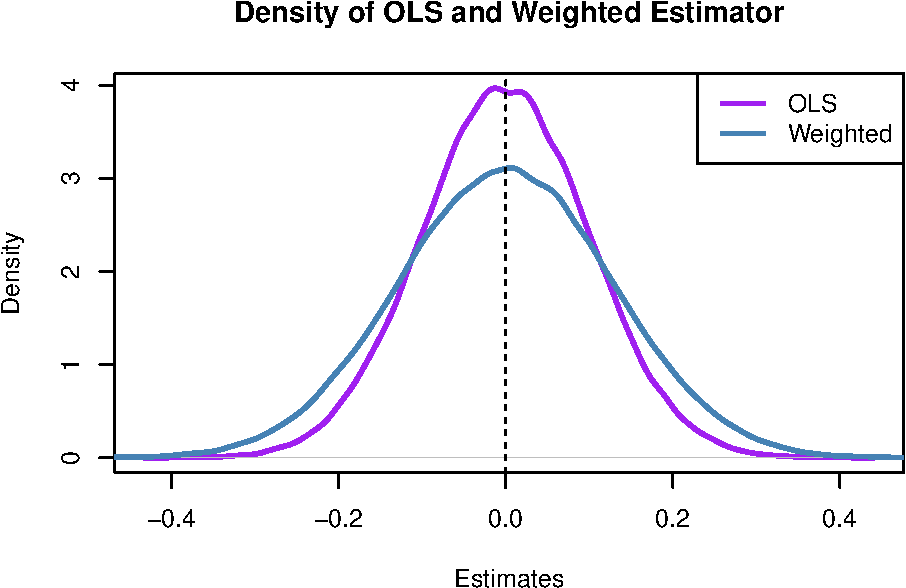
\includegraphics{URFITE_files/figure-latex/unnamed-chunk-125-1} \end{center}

The outcomes are consistent with our expectations: the empirical
distributions of both estimators seem to track the \(t_{18}\)
distribution quite closely.

\chapter{Regression Models with Multiple
Regressors}\label{regression-models-with-multiple-regressors}

In what follows we introduce linear regression models that use more than
just one explanatory variable and discuss important key concepts in
multiple regression. As we broaden our scope beyond the relationship of
only two variables (dependent and independent variable), some potential
issues arise, such as multicollinearity and omitted variable bias. In
particular, this chapter deals with omitted variables and their hazard
to causal interpretation of OLS-estimated coefficients. Naturally, we
will introduce estimation of multiple regression models using R. We will
also advocate thoughtful usage of multiple regression models by
simulation sudies in R that demonstrate consequences of using highly
correlated regressors or a misspecified model.

\section{Omitted Variable Bias}\label{omitted-variable-bias}

Previous analysis of the relationship between test score and class size
discussed in Chapters 4 and 5 has a major flaw: we ignored other
potentially important determinants of test scores that vary with our
regressor. The influences of those variables were collected in the error
term. This might induce an estimation bias, i.e.~the mean of the OLS
estimator's sampling distribution is no longer equal to the true mean
and we measure a wrong effect on test scores of a unit change in the
student-teacher ratio. This is called omitted variable bias, see Key
Concept 6.1.

Key Concept 6.1

Omitted Variable Bias in Regression with a Single Regressor

Omitted variable bias is the bias in the OLS estimator that arises when
the regressor, \(X\), is \emph{correlated} with an omitted variable. For
omitted variable bias to occur, two conditions must be fulfilled:

\begin{enumerate}
\def\labelenumi{\arabic{enumi}.}
\tightlist
\item
  \(X\) is correlated with the omitted variable.
\item
  The omitted variable is a determinant of the dependent variable \(Y\).
\end{enumerate}

Together, 1. and 2. result in a violation of the first OLS assumption
\(E(u_i\vert X_i) = 0\). Formally, the resulting bias can be expressed
as

\[ \hat\beta_1 \xrightarrow[]{p} \beta_1 + \rho_{Xu} \frac{\sigma_u}{\sigma_X}. \tag{6.1} \]
See Appendix 6.1 in the book for a detailed derivation. (6.1) states
that OVB is a problem that cannot be aleviated by increasing the numner
of observations used to estimate \(\beta_1\) since then \(\hat\beta_1\)
is inconsistent: OVB prevents the estimator to converge in probability
to the true parameter value. Strength and direction of the bias are
driven by \(\rho_{Xu}\), the correlation between the error term and the
regressor.

In our example of test score and class size, it is fairly easy to come
up with variables that may cause such a bias if omitted. As mentioned in
the book, a highly relevant variable could be the percentage of english
learners in the school district: it is plausible that the ability to
speak, read and write english is an important factor for successful
learning. Therefore, students that are still learning english are likely
to perform worse in the tests than native speakers are. Also, it is
conceivable that the share of english learning students is larger in
school districts where class sizes are large. Think of less well-off
urban districs were a lot of immigrants live.

Let us think about a possible bias induced by omitting the share of
english learning students (\(PctEL\)) in view of (6.1) when the
estimated regression model excludes \(PctEL\) although the true DGP is

\[ TestScore = \beta_0 + \beta_1 \times STR + \beta_2 \times PctEL \tag{6.2}\]

where \(STR\) and \(PctEL\) are correlated,

\[corr(STR,PctEL)\neq0.\]

After defining our variables in R, we compute the correlation between
\(STR\) and \(PctEL\) as well as the correlation between \(STR\) and
\(TestScore\).

\begin{Shaded}
\begin{Highlighting}[]
\CommentTok{# load the AER package}
\KeywordTok{library}\NormalTok{(AER)}

\CommentTok{# load the data set}
\KeywordTok{data}\NormalTok{(CASchools)   }

\CommentTok{# define variables}
\NormalTok{CASchools}\OperatorTok{$}\NormalTok{STR <-}\StringTok{ }\NormalTok{CASchools}\OperatorTok{$}\NormalTok{students}\OperatorTok{/}\NormalTok{CASchools}\OperatorTok{$}\NormalTok{teachers       }
\NormalTok{CASchools}\OperatorTok{$}\NormalTok{score <-}\StringTok{ }\NormalTok{(CASchools}\OperatorTok{$}\NormalTok{read }\OperatorTok{+}\StringTok{ }\NormalTok{CASchools}\OperatorTok{$}\NormalTok{math)}\OperatorTok{/}\DecValTok{2}

\CommentTok{# compute correlations}
\KeywordTok{cor}\NormalTok{(CASchools}\OperatorTok{$}\NormalTok{STR, CASchools}\OperatorTok{$}\NormalTok{score)}
\end{Highlighting}
\end{Shaded}

\begin{verbatim}
## [1] -0.2263627
\end{verbatim}

\begin{Shaded}
\begin{Highlighting}[]
\KeywordTok{cor}\NormalTok{(CASchools}\OperatorTok{$}\NormalTok{STR, CASchools}\OperatorTok{$}\NormalTok{english)}
\end{Highlighting}
\end{Shaded}

\begin{verbatim}
## [1] 0.1876424
\end{verbatim}

The fact that \(\widehat{corr}(STR, Testscore) = -0.2264\) is cause for
concern that omitting \(PctEL\) leads to a negatively biased estimate
\(\hat\beta_1\) since then \(\rho_{Xu} < 0\) and we have \(\sigma_X>0\),
\(\sigma_u>0\) by definition. As consequence we expect \(\hat\beta_1\),
the coefficient on \(STR\), to be too large in absolute value. Put
differently, the OLS estimate of \(\hat\beta_1\) suggests that small
classes improve test scores but the estimated effect of small classes is
too strong as it captures the effect of having fewer English learners,
too.

What happens to the magnitude of \(\hat\beta_1\) if we add the variable
\(PctEL\) to the regression, that is if we estimate the model
\[ TestScore = \beta_0 + \beta_1 \times STR + \beta_2 \times PctEL + u \]

instead? And what do we expect about the sign of, \(\hat\beta_2\), the
estimated coefficient on \(PctEL\)? Following the reasoning above we
should end up with a (still) negative but larger coefficient estimate
\(\hat\beta_1\) and a negative estimate \(\hat\beta_2\).

Let us estimate both regression models and compare. Performing a
multiple regression in R is straightforward. One can simply add
additional variables to the right hand side of the \texttt{formula}
argument of the function \texttt{lm()} by using their names and the
\texttt{+} operator. Notice that \texttt{english} is the name of the
column in the data set \texttt{CASchools} which contains observations on
the share of English learning students.

\begin{Shaded}
\begin{Highlighting}[]
\CommentTok{# estimate both regression models}
\NormalTok{mod <-}\StringTok{ }\KeywordTok{lm}\NormalTok{(score }\OperatorTok{~}\StringTok{ }\NormalTok{STR, }\DataTypeTok{data =}\NormalTok{ CASchools) }
\NormalTok{mult.mod <-}\StringTok{ }\KeywordTok{lm}\NormalTok{(score }\OperatorTok{~}\StringTok{ }\NormalTok{STR }\OperatorTok{+}\StringTok{ }\NormalTok{english, }\DataTypeTok{data =}\NormalTok{ CASchools)}

\NormalTok{mod}
\end{Highlighting}
\end{Shaded}

\begin{verbatim}
## 
## Call:
## lm(formula = score ~ STR, data = CASchools)
## 
## Coefficients:
## (Intercept)          STR  
##      698.93        -2.28
\end{verbatim}

\begin{Shaded}
\begin{Highlighting}[]
\NormalTok{mult.mod}
\end{Highlighting}
\end{Shaded}

\begin{verbatim}
## 
## Call:
## lm(formula = score ~ STR + english, data = CASchools)
## 
## Coefficients:
## (Intercept)          STR      english  
##    686.0322      -1.1013      -0.6498
\end{verbatim}

We find the outcomes to be consistent with our expectations. The
following section discusses some thoery on multiple regression models.

\section{The Multiple Regression
Model}\label{the-multiple-regression-model}

In a multiple regression model we extend the basic concept of the simple
regression model discussed in Chapter 4 and 5. A multiple regression
model enables us to estimate the effect on \(Y_i\) of changing a
regressor \(X_{1i}\) if the remaining regressors
\(X_{2i},X_{3i}\dots,X_{ki}\) \emph{do not vary}. In fact we already
have performed estimation of the multiple regression model (6.2) using R
in the previous section. Recall that the interpretation of the
coefficient on student-teacher ratio is the effect on test scores of a
one unit change student-teacher ratio if the percentage of English
learners is kept constant.

As in the simple regression model, we assume the true relationship
between \(Y\) and \(X_{2i},X_{3i}\dots\) to be linear. On average, this
relation is given by the population regression function

\[ E(Y_i\vert X_{1i}=x_1, X_{2i}=x_2,  X_{3i}=x_3,\dots, X_{ki}=x_k) = \beta_0 + \beta_1 x_1 + \beta_2 x_2 + \beta_3 x_3 + \dots + \beta_k x_k. \tag{6.3} \]

As in the simple regression model, this relation does not hold exactly
since there are disturbing influences to the dependent variable \(Y\) we
cannot observe as explanatory variables. Therefore we add an error term
\(u\) which represents deviations of the observations from the
population regression line to (6.3). This yields the population multiple
regression model

\[ Y_i = \beta_0 + \beta_1 X_{1i} + \beta_2 X_{2i} + \beta_3 X_{3i} + \dots + \beta_k X_{ki} + u_i \ \ , \ \ i=1,\dots,n. \tag{6.4} \]

Key Concept 6.2

The Multiple Regression Model

The multiple regression model is

\[ Y_i = \beta_0 + \beta_1 X_{1i} + \beta_2 X_{2i} + \beta_3 X_{3i} + \dots + \beta_k X_{ki} + u_i \ \ , \ \ i=1,\dots,n.  \]

Designations are similar to those in the simple regression model:

\begin{itemize}
\tightlist
\item
  \(Y_i\) is the \(i^{th}\) observation in the dependent variable.
  Observations on the \(k\) regressors are denoted by
  \(X_{1i},X_{2i},\dots,X_{ki}\) and \(u_i\) is the error term.
\item
  The average relationship between \(Y\) and the regressors is given by
  the population regression line
  \[ E(Y_i\vert X_{1i}=x_1, X_{2i}=x_2,  X_{3i}=x_3,\dots, X_{ki}=x_k) = \beta_0 + \beta_1 x_1 + \beta_2 x_2 + \beta_3 x_3 + \dots + \beta_k x_k. \]
\item
  \(\beta_0\) is the intercept; it is the expected value of \(Y\) when
  all \(X\)s equal \(0\). \(\beta_j \ , \ j=1,\dots,k\) are the
  coefficients on \(X_j \ , \ j=1,\dots,k\). \(\beta_1\) measures the
  expected change in \(Y_i\) that results from a one unit change in
  \(X_{1i}\) while holding all other regressors \(X_{ji} \ , \ j\neq1\)
  constant.
\end{itemize}

Key Concept 6.2 summarizes the core concepts of the multiple regression
model. How can we estimate the coefficients of the multiple regression
model (6.4)? We will not go to much into detail on this issue as our
focus lies on usage of R instead of the technical refinements. However
it should be pointed out that, similarly to the simple regression model,
the coefficients of the multiple regression model can be estimated using
OLS. As in the simple model, we seek to minimize the sum of squared
prediction mistakes by choosing estimates \(b_0,b_1,\dots,b_k\) for the
coefficients \(\beta_0,\beta_1,\dots,\beta_k\) such that

\[\sum_{i=1}^n (Y_i - b_0 - b_1 X_{1i} - b_2 X_{2i} - \dots -  b_k X_{ki})^2 \tag{6.5}\]

is minimized. Note that (6.5) is simply an extension of \(SSR\) in the
case with just one regressor and an intercept. The estimators that
minimize (6.5) are hence denoted
\(\hat\beta_0,\hat\beta_1,\dots,\hat\beta_k\) and, as in the simple
regression model, we call them the ordinary least squares estimators of
\(\beta_0,\beta_1,\dots,\beta_k\). For the predicted value of \(Y_i\)
given the regressors and the estimates
\(\hat\beta_0,\hat\beta_1,\dots,\hat\beta_k\) we have

\[ \hat{Y}_i = \hat\beta_0 + \hat\beta_1 X_{1i} + \dots +\hat\beta_k X_{ki}. \]
and, as before, the difference of \(Y_i\) and its predicted value
\(\hat{Y}_i\) is called the OLS residual of observation \(i\):
\(\hat{u} = Y_i - \hat{Y}_i\).

 For further information regarding the theory behind multiple
regression, see Chapter 18.1 in the book which inter alia presents a
derivation of the OLS estimator in the multiple regression model using
matrix notation.

Now let us jump back to the example of test scores and class sizes. The
estimated model object is \texttt{mult.mod}. As for simple regression
models we can use the \texttt{summary()} function to obtain information
on estimated coefficients and model statistics.

\begin{Shaded}
\begin{Highlighting}[]
\KeywordTok{summary}\NormalTok{(mult.mod)}\OperatorTok{$}\NormalTok{coef}
\end{Highlighting}
\end{Shaded}

\begin{verbatim}
##                Estimate Std. Error    t value      Pr(>|t|)
## (Intercept) 686.0322445 7.41131160  92.565565 3.871327e-280
## STR          -1.1012956 0.38027827  -2.896026  3.978059e-03
## english      -0.6497768 0.03934254 -16.515882  1.657448e-47
\end{verbatim}

So the estimated multiple regression model is

\[ \widehat{TestScore} = \underset{(7.41)}{686.03} - \underset{(0.38)}{1.10} \times STR - \underset{(0.04)}{0.65} \times PctEL \tag{6.6}.  \]

Unlike in the simple regression model where the data can be represented
by points in the two-dimensional cartesian coordinate system, we are now
dealing with three dimensions. Hence observations can be represented by
points in the three-dimensional real space, denoted \(\mathbb{R}^3\).
Therefore (6.6) is now longer a regression line but a \emph{regression
plane}. This idea extends to higher dimensions when we further expand
the number of regressors \(k\). We then say that the regression model
can be represented a hyperplane in the \(k+1\) dimensional space. It is
already hard to imagine such a space if \(k=3\) and we best stick with
the general idea that, in the multiple regression model, the dependent
variable is explained by a \emph{linear combination of the regressors}.
However, in the present case we are able to visualize the situation. The
following figure is an interactive 3D visualization of the data and the
estimated regression plane (6.6).

\hypertarget{14f931e9bc8dd}{}

We observe that the estimated regression plane fits the data reasonably
well --- at least with regard to the shape and spatial poistion of the
point cloud. The color of the markers is an indicator for the absolute
deviation from the predicted regression plane. Observations that are
coloured more reddish lie close to the regression plane while the color
shifts to blue with growing distance. An anomaly that can be seen from
the plot is that there might be heteroskedasticity: we see that the
dispersion of regression errors made, i.e.~the distance of observations
to the regression plane shows a tendency to decrease as the share of
English learning students increases.

\section{Measures of Fit in Multiple
Regression}\label{measures-of-fit-in-multiple-regression}

In multiple regression, common summary statistics are \(SER\),
\(R\)\^{}2 and the adjusted \(R^2\).

Taking the code from Section 6.3 You could simply use
\texttt{summary(mult.mod)} to print the \(SER\), \(R^2\) and
adjusted-\(R^2\). For multiple regression models the \(SER\) is computed
as

\[ SER = s_{\hat u} = \sqrt{s_{\hat u}^2} \] where, in contrast to the
simple regression model we apply a modification to the denominator of
the premultiplied factor in \(s_{\hat u}^2\) in order to accommodate for
additional regressors. Thus,

\[ s_{\hat u}^2 = \frac{1}{n-k-1} \, SSR \]

with \(k\) the number of regressors \emph{excluding} the intercept.
While \texttt{summary()} computes the \(R^2\) just as in the case of a
single regressor, it is not a reliable measure for multiple regression
models. This is due to \(R^2\) becoming larger every time an additional
regressor is added to the model since adding a regressor decreases the
\(SSR\) --- at least unless the respective estimated coefficient is
exactly zero what practically never happens to be the case (see chapter
6.4 in the book). The adjusted \(R^2\) takes this into consideration by
``punishing'' the addition of regressors using a correction factor. So
the adjusted \(R^2\) or simply \(\overline{R^2}\) is a modified version
of \(R^2\).

\[ \overline{R^2} = 1-\frac{n-1}{n-k-1} \, \frac{SSR}{TSS} \]

As You may have already suspected, \texttt{summary()} adjusts the
formula for \(SER\) by itself and it computes \(\overline{R^2}\) and of
course \(R^2\) by default, therby leaving the decision which measure to
rely on up to the user.

You can find the measures at the bottom of the output produced by
calling \texttt{summary(mult.mod)}.

\begin{Shaded}
\begin{Highlighting}[]
\KeywordTok{summary}\NormalTok{(mult.mod)}
\end{Highlighting}
\end{Shaded}

\begin{verbatim}
## 
## Call:
## lm(formula = score ~ STR + english, data = CASchools)
## 
## Residuals:
##     Min      1Q  Median      3Q     Max 
## -48.845 -10.240  -0.308   9.815  43.461 
## 
## Coefficients:
##              Estimate Std. Error t value Pr(>|t|)    
## (Intercept) 686.03224    7.41131  92.566  < 2e-16 ***
## STR          -1.10130    0.38028  -2.896  0.00398 ** 
## english      -0.64978    0.03934 -16.516  < 2e-16 ***
## ---
## Signif. codes:  0 '***' 0.001 '**' 0.01 '*' 0.05 '.' 0.1 ' ' 1
## 
## Residual standard error: 14.46 on 417 degrees of freedom
## Multiple R-squared:  0.4264, Adjusted R-squared:  0.4237 
## F-statistic:   155 on 2 and 417 DF,  p-value: < 2.2e-16
\end{verbatim}

We can also compute the measures by hand using the formulas above. Let
us check if the results coincide with the values provided by
\texttt{summary()}.

\begin{Shaded}
\begin{Highlighting}[]
\CommentTok{# define the components}
\NormalTok{n <-}\StringTok{ }\KeywordTok{nrow}\NormalTok{(CASchools)                            }\CommentTok{# number of observations (rows)}
\NormalTok{k <-}\StringTok{ }\DecValTok{2}                                          \CommentTok{# number of regressors}

\NormalTok{y_mean <-}\StringTok{ }\KeywordTok{mean}\NormalTok{(CASchools}\OperatorTok{$}\NormalTok{score)                 }\CommentTok{# mean of avg. test-scores}

\NormalTok{SSR <-}\StringTok{ }\KeywordTok{sum}\NormalTok{(}\KeywordTok{residuals}\NormalTok{(mult.mod)}\OperatorTok{^}\DecValTok{2}\NormalTok{)               }\CommentTok{# sum of squared residuals}
\NormalTok{TSS <-}\StringTok{ }\KeywordTok{sum}\NormalTok{((CASchools}\OperatorTok{$}\NormalTok{score }\OperatorTok{-}\StringTok{ }\NormalTok{y_mean )}\OperatorTok{^}\DecValTok{2}\NormalTok{)       }\CommentTok{# total sum of squares}
\NormalTok{ESS <-}\StringTok{ }\KeywordTok{sum}\NormalTok{((}\KeywordTok{fitted}\NormalTok{(mult.mod) }\OperatorTok{-}\StringTok{ }\NormalTok{y_mean)}\OperatorTok{^}\DecValTok{2}\NormalTok{)       }\CommentTok{# explained sum of squares}

\CommentTok{# compute the measures}

\NormalTok{SER <-}\StringTok{ }\KeywordTok{sqrt}\NormalTok{(}\DecValTok{1}\OperatorTok{/}\NormalTok{(n}\OperatorTok{-}\NormalTok{k}\OperatorTok{-}\DecValTok{1}\NormalTok{) }\OperatorTok{*}\StringTok{ }\NormalTok{SSR)                    }\CommentTok{# standard error of the regression}
\NormalTok{Rsq <-}\StringTok{ }\DecValTok{1} \OperatorTok{-}\StringTok{ }\NormalTok{(SSR }\OperatorTok{/}\StringTok{ }\NormalTok{TSS)                          }\CommentTok{# R^2}
\NormalTok{adj_Rsq <-}\StringTok{ }\DecValTok{1} \OperatorTok{-}\StringTok{ }\NormalTok{(n}\OperatorTok{-}\DecValTok{1}\NormalTok{)}\OperatorTok{/}\NormalTok{(n}\OperatorTok{-}\NormalTok{k}\OperatorTok{-}\DecValTok{1}\NormalTok{) }\OperatorTok{*}\StringTok{ }\NormalTok{SSR}\OperatorTok{/}\NormalTok{TSS          }\CommentTok{# adj. R^2}

\CommentTok{# Print the measures to the console}
\KeywordTok{c}\NormalTok{(}\StringTok{"SER"}\NormalTok{ =}\StringTok{ }\NormalTok{SER, }\StringTok{"R2"}\NormalTok{ =}\StringTok{ }\NormalTok{Rsq, }\StringTok{"Adj.R2"}\NormalTok{ =}\StringTok{ }\NormalTok{adj_Rsq)}
\end{Highlighting}
\end{Shaded}

\begin{verbatim}
##        SER         R2     Adj.R2 
## 14.4644831  0.4264315  0.4236805
\end{verbatim}

We find that the results do match. Now, what can be said about the fit
of our multiple regression model for test scores with the percentage of
english learners as an additional regressor? Does it improve on the
simple model including only an intercept and a measure of the class
size? The answer is yes: this is easily seen by comparing these measures
of fit with those for the simple regression model \texttt{mod}.

\begin{Shaded}
\begin{Highlighting}[]
\CommentTok{# SER}
\KeywordTok{summary}\NormalTok{(mod)}\OperatorTok{$}\NormalTok{sigma}
\end{Highlighting}
\end{Shaded}

\begin{verbatim}
## [1] 18.58097
\end{verbatim}

\begin{Shaded}
\begin{Highlighting}[]
\CommentTok{# R^2}
\KeywordTok{summary}\NormalTok{(mod)}\OperatorTok{$}\NormalTok{r.squared}
\end{Highlighting}
\end{Shaded}

\begin{verbatim}
## [1] 0.05124009
\end{verbatim}

\begin{Shaded}
\begin{Highlighting}[]
\CommentTok{# Adj. R^2}
\KeywordTok{summary}\NormalTok{(mod)}\OperatorTok{$}\NormalTok{adj.r.squared}
\end{Highlighting}
\end{Shaded}

\begin{verbatim}
## [1] 0.04897033
\end{verbatim}

Including \(PctEL\) as a regressor boots the \(R^2\) from about \(5\%\)
to \(42.6\%\). Qualitatively the same is observed for \(\overline{R^2}\)
which we deem to be more reliable in view of the discussion above.
Notice that the difference between \(R^2\) and \(\overline{R^2}\) is
small since \(k=2\) and \(n\) is large. Condensed, the fit of (6.6)
improves vastly on the fit of the simple regression model with \(STR\)
as the only regressor. Comparing prediction errors we find that the
prediction precision of the multiple regression model (6.6) improves
upon the simple model as adding \(PctEL\) lowers the \(SER\) from
\(18.6\) to \(14.5\) units of test score.

 As already mentioned \(R^2\) and \(\overline{R^2}\) may be used to
quantify how good a model fits the data. However it is rarely a good
idea to maximize these measures by stuffing the model with regressors in
general. You will (hopefully) not find any serious study that does so.
Instead it is more fruitful to include regressors that improve
estimation of the causal effect of interest which is \emph{not} assessed
by means of a low \(SSR\). The issue of variable selection is covered in
Chapter 7 of this script and Chapter 7 in the book.

\section{OLS Assumptions in Multiple
Regression}\label{ols-assumptions-in-multiple-regression}

In the multiple regression model we extend the known three least squares
assumptions imposed for the simple regression model (see
\protect\hyperlink{ch4}{Chapter 4}, Key Concept 4.3) and add a fourth
assumption. These assumptions are presented in Key Concept 6.4. While we
will not go into the details of assumptions 1, 2 and 3 since their ideas
have been discussed before and are easily generalized to the case of
multiple regressors, we will devote our attention to the fourth
assumption. This forth assumption forbids the occurence of perfect
correlation between any pair of regressors.

Key Concept 6.4

The Least Squares Assumptions in the Multiple Regression Model

The multiple regression model is given by

\[ Y_i = \beta_0 + \beta_1 X_{1i} + \beta_1 X_{2i} + \dots + \beta_k X_{ki} + u_i \ , \ i=1,\dots,n. \]

The OLS assumptions in the multiple regression model are an extension of
the ones made for the simple regression model:

\begin{enumerate}
\def\labelenumi{\arabic{enumi}.}
\tightlist
\item
  Regressors \((X_{1i}, X_{2i}, \dots, X_{ki}, Y_i) \ , \ i=1,\dots,n\)
  are drawn such that the i.i.d. assumption holds.
\item
  \(u_i\) is an error term with conditional zero given the regressors,
  i.e. \[ E(u_i\vert X_{1i}, X_{2i}, \dots, X_{ki}) = 0. \]
\item
  Large outliers are unlikely, formally \(X_{1i},\dots,X_{ki}\) and
  \(Y_i\) have finite fourth moments.
\item
  No perfect multicollinearity.
\end{enumerate}

\subsection*{Multicollinearity}\label{multicollinearity}
\addcontentsline{toc}{subsection}{Multicollinearity}

If two or more regressors in a multiple regression model are
\emph{strongly} correlated we say that there is
\emph{multicollinearity}. If the correlation between two or more
regressors is perfect (correlation coeficient equals \(1\)), we refer to
the situation as \emph{perfect multicollinearity}. Perfectly
multicollinear regressors can be written as linear combinations of each
other. While strong multicollinearity in general is unpleasent as it
causes the variance of the OLS estimator to be large (we will discuss is
in more detail later), the presence of perfect multicollinearity makes
it even impossible to solve for the OLS estimator, that is the model
cannot be estimated at all.

The next section presents some examples of perfect multicollinearity and
demonstrates how R, specifically the \texttt{lm} function deals with
them.

\subsubsection*{Examples of Perfect
Multicollinearity}\label{examples-of-perfect-multicollinearity}
\addcontentsline{toc}{subsubsection}{Examples of Perfect
Multicollinearity}

How does R react if we want it to estimate a model with perfectly
correlated regressors?

If we use the \texttt{lm} function to estimate a model with a set of
regressors that suffer from perfect multicollinearity the system will
produce a warning in the first line of the coefficient section of the
output (1 not defined because of singularities) and ignore the
regressor(s) which is (are) assumed to be a linear combination of the
others. See the following example where we add another variable
\texttt{FracEL}, the fraction of Englisch learners to \texttt{CASchools}
where observations are scaled values of the observations for
\texttt{english} and use it as a regressor together with \texttt{STR}
and \texttt{english} in a multiple regression model. In this example
\texttt{english} and \texttt{FracEL} are perfectly collinear. The R code
is as follows.

\begin{Shaded}
\begin{Highlighting}[]
\CommentTok{# define the fraction of english learners        }
\NormalTok{CASchools}\OperatorTok{$}\NormalTok{FracEL <-}\StringTok{ }\NormalTok{CASchools}\OperatorTok{$}\NormalTok{english}\OperatorTok{/}\DecValTok{100}

\CommentTok{# estimate the model}
\NormalTok{mult.mod <-}\StringTok{ }\KeywordTok{lm}\NormalTok{(score }\OperatorTok{~}\StringTok{ }\NormalTok{STR }\OperatorTok{+}\StringTok{ }\NormalTok{english }\OperatorTok{+}\StringTok{ }\NormalTok{FracEL, }\DataTypeTok{data =}\NormalTok{ CASchools) }

\CommentTok{# obtain a summary of the model}
\KeywordTok{summary}\NormalTok{(mult.mod)                                                 }
\end{Highlighting}
\end{Shaded}

\begin{verbatim}
## 
## Call:
## lm(formula = score ~ STR + english + FracEL, data = CASchools)
## 
## Residuals:
##     Min      1Q  Median      3Q     Max 
## -48.845 -10.240  -0.308   9.815  43.461 
## 
## Coefficients: (1 not defined because of singularities)
##              Estimate Std. Error t value Pr(>|t|)    
## (Intercept) 686.03224    7.41131  92.566  < 2e-16 ***
## STR          -1.10130    0.38028  -2.896  0.00398 ** 
## english      -0.64978    0.03934 -16.516  < 2e-16 ***
## FracEL             NA         NA      NA       NA    
## ---
## Signif. codes:  0 '***' 0.001 '**' 0.01 '*' 0.05 '.' 0.1 ' ' 1
## 
## Residual standard error: 14.46 on 417 degrees of freedom
## Multiple R-squared:  0.4264, Adjusted R-squared:  0.4237 
## F-statistic:   155 on 2 and 417 DF,  p-value: < 2.2e-16
\end{verbatim}

Notice that the row \texttt{FracEL} in the coefficients section of the
output consists of \texttt{NA} entries since \texttt{FracEL} was
excluded from the model.

If we were to compute OLS by hand we would run into the problem as well
but no one would be helping us out! The computation simply fails. Why is
this the case? Take the following example:

Assume You want to estimate a simple linear regression model with an
intercept and one regressor:

\[ Y_i = \beta_0 + \beta_1 X_i + u_i\]

As mentioned above, for perfect multicollinearity to be present \(X\)
has to be a linear combination of the other regressors. Since the only
other regressor is a constant (think of the right hand side of the model
equation as \(\beta_0 \times 1 + \beta_1 X_i + u_i\) so that \(\beta_1\)
is always multiplied by \(1\) for every observation), \(X\) has to be
constant as well. When we recap the formula for \(\hat\beta_1\) and
rewrite it somewhat, we have

\[ \hat{\beta_1} =  \frac{\sum_{i = 1}^n (X_i - \bar{X})(Y_i - \bar{Y})} { \sum_{i=1}^n (X_i - \bar{X})^2} = \frac{\frac{1}{n-1} \sum_{i = 1}^n (X_i - \bar{X})(Y_i - \bar{Y})} {\frac{1}{n-1} \sum_{i=1}^n (X_i - \bar{X})^2} = \frac{\widehat{cov}(X,Y)}{\widehat{Var}(X)}. \tag{6.7} \]

So the variance of the regressor \(X\) stands in the denominator. Since
the variance of a constant is zero, we are not able to compute this
fraction and \(\hat{\beta}_1\) remains undefined.

Note: In this special case the nominator in (6.7) equal zero, too. Can
You show that?

Let us behold two further examples where our selection of regressors
induces perfect multicollinearity. First, assume that we intend to
analyse the effect of class size on test score by using a dummy variable
that identifies ``Not very small'' classes (NVS). We define that a
school has the NVS attribute when the school's average student-teacher
ratio is at least \(12\).

\[ NVS = \begin{cases} 0 \ \ \ \text{if STR < 12} \\ 1 \ \ \ \text{otherwise} \end{cases} \]

We add the corresponding column to \texttt{CASchools} and estimate a
multiple regression model with covariates \texttt{computer} and
\texttt{english}.

\begin{Shaded}
\begin{Highlighting}[]
\CommentTok{# if STR smaller 12, NVS = 0, else NVS = 1}
\NormalTok{CASchools}\OperatorTok{$}\NormalTok{NVS <-}\StringTok{ }\KeywordTok{ifelse}\NormalTok{(CASchools}\OperatorTok{$}\NormalTok{STR }\OperatorTok{<}\StringTok{ }\DecValTok{12}\NormalTok{, }\DecValTok{0}\NormalTok{, }\DecValTok{1}\NormalTok{)}

\CommentTok{# estimate the model}
\NormalTok{mult.mod <-}\StringTok{ }\KeywordTok{lm}\NormalTok{(score }\OperatorTok{~}\StringTok{ }\NormalTok{computer }\OperatorTok{+}\StringTok{ }\NormalTok{english }\OperatorTok{+}\StringTok{ }\NormalTok{NVS, }\DataTypeTok{data =}\NormalTok{ CASchools)}

\CommentTok{# obtain a model summary}
\KeywordTok{summary}\NormalTok{(mult.mod)                                                  }
\end{Highlighting}
\end{Shaded}

\begin{verbatim}
## 
## Call:
## lm(formula = score ~ computer + english + NVS, data = CASchools)
## 
## Residuals:
##     Min      1Q  Median      3Q     Max 
## -49.492  -9.976  -0.778   8.761  43.798 
## 
## Coefficients: (1 not defined because of singularities)
##               Estimate Std. Error t value Pr(>|t|)    
## (Intercept) 663.704837   0.984259 674.319  < 2e-16 ***
## computer      0.005374   0.001670   3.218  0.00139 ** 
## english      -0.708947   0.040303 -17.591  < 2e-16 ***
## NVS                 NA         NA      NA       NA    
## ---
## Signif. codes:  0 '***' 0.001 '**' 0.01 '*' 0.05 '.' 0.1 ' ' 1
## 
## Residual standard error: 14.43 on 417 degrees of freedom
## Multiple R-squared:  0.4291, Adjusted R-squared:  0.4263 
## F-statistic: 156.7 on 2 and 417 DF,  p-value: < 2.2e-16
\end{verbatim}

Again, the output of \texttt{summary(mult.mod)} tells us that inclusion
of \texttt{NVS} in the regression would render the estimation
infeasible. What happened here? This is an example where we made a
logical mistake when defining the regressor \texttt{NVS}: if we had
taken a closer look at \texttt{NVS}, the redefined measure for class
size, we would have noticed that there is not a single school with
\(STR<12\) hence \(NVS\) equals one for all observations. We can check
this by printing the contents of \texttt{CASchools\$NVS} to the console
or by using the function \texttt{table}, see \texttt{?table}.

\begin{Shaded}
\begin{Highlighting}[]
\KeywordTok{table}\NormalTok{(CASchools}\OperatorTok{$}\NormalTok{NVS)}
\end{Highlighting}
\end{Shaded}

\begin{verbatim}
## 
##   1 
## 420
\end{verbatim}

\texttt{CASchools\$NVS} is a vector of \(420\) ones and our data set
includes \(420\) observations. This obviously violates assumption 4 of
Key Concept 6.4: remember that observations for the intercept are always
\(1\) so we have

\begin{align}
  intercept = \, & \lambda \cdot NVS \\
  \\
  \begin{pmatrix} 1 \\ \vdots \\ 1\end{pmatrix} = \, & \lambda \cdot \begin{pmatrix} 1 \\ \vdots \\ 1\end{pmatrix} \\   \Leftrightarrow \, & \lambda = 1.
\end{align}

Since both regressors can be written as a linear combination of each
other, we face perfect multicollinearity and R excludes \(NVS\) from the
model. Thus the message to take away is: think carefully about how
regressors You created Yourself could possibly interact with
unrecognized features of the data set!

Another example of perfect multicollinearity is known as the ``dummy
variable trap''. This may occur when multiple dummy variables are used
as regressors. A common case for this is when the dummies are used to
sort the data set into mutually exclusive categories. For example,
suppose we have spatial information that indicates whether a school is
located in the North, West, South or East of the US which allows us to
create the dummy variables

\begin{align}
  North_i =& 
  \begin{cases}
    1 \ \ \text{if located in the north} \\
    0 \ \ \text{otherwise}
  \end{cases} \\
  \\
    West_i =& 
  \begin{cases}
    1 \ \ \text{if located in the west} \\
    0 \ \ \text{otherwise}
  \end{cases} \\
  \\
    South_i =& 
  \begin{cases}
    1 \ \ \text{if located in the south} \\
    0 \ \ \text{otherwise}
  \end{cases} \\
    \\
    East_i =& 
  \begin{cases}
    1 \ \ \text{if located in the east} \\
    0 \ \ \text{otherwise}.
  \end{cases}
\end{align}

Since the directions are mutually exclusive, for every school
\(i=1,\dots,n\) we have

\[ North_i + West_i + South_i + East_i = 1. \]

We run into problems when trying to estimate a model that includes a
constant and \emph{all four} direction dummies, e.g.~in the model

\[ TestScore = \beta_0 + \beta_1 \times STR + \beta_2 \times english + \beta_3 \times North_i + \beta_4 \times West_i + \beta_5 \times South_i + \beta_6 \times East_i + u_i \tag{6.8}\]
since then for all observations \(i=1,\dots,n\) the constant term can be
written as a linear combination of the dummies:

\begin{align}
  intercept = \, & \lambda_1 \cdot (North + West + South + East) \\
  \\
  \begin{pmatrix} 1 \\ \vdots \\ 1\end{pmatrix} = \, & \lambda \cdot \begin{pmatrix} 1 \\ \vdots \\ 1\end{pmatrix} \\   \Leftrightarrow \, & \lambda = 1
\end{align}

and we have perfect multicollinearity. This is what is meant by the
``dummy variable trap'': not paying attention and erroneously including
all dummies and an intercept term in a regression model.

How does the \texttt{lm} function in R handle a regression like (6.8)?
To answer this we first generate some artifical categorical data and
append a new column named \texttt{directions} to \texttt{CASchools} and
see what \texttt{lm} does when asked to estimate the model above.

\begin{Shaded}
\begin{Highlighting}[]
\CommentTok{# set random seed for reproducibility}
\KeywordTok{set.seed}\NormalTok{(}\DecValTok{1}\NormalTok{)}

\CommentTok{# Generate artificial data on location}
\NormalTok{CASchools}\OperatorTok{$}\NormalTok{direction <-}\StringTok{ }\KeywordTok{sample}\NormalTok{(}\KeywordTok{c}\NormalTok{(}\StringTok{"West"}\NormalTok{,}\StringTok{"North"}\NormalTok{,}\StringTok{"South"}\NormalTok{,}\StringTok{"East"}\NormalTok{), }\DecValTok{420}\NormalTok{, }\DataTypeTok{replace =}\NormalTok{ T)}

\CommentTok{# estimate the model}
\NormalTok{mult.mod <-}\StringTok{ }\KeywordTok{lm}\NormalTok{(score }\OperatorTok{~}\StringTok{ }\NormalTok{STR }\OperatorTok{+}\StringTok{ }\NormalTok{english }\OperatorTok{+}\StringTok{ }\NormalTok{direction, }\DataTypeTok{data =}\NormalTok{ CASchools)}

\CommentTok{# obtain a model summary}
\KeywordTok{summary}\NormalTok{(mult.mod)                                                 }
\end{Highlighting}
\end{Shaded}

\begin{verbatim}
## 
## Call:
## lm(formula = score ~ STR + english + direction, data = CASchools)
## 
## Residuals:
##     Min      1Q  Median      3Q     Max 
## -48.018 -10.098  -0.556   9.304  42.596 
## 
## Coefficients:
##                 Estimate Std. Error t value Pr(>|t|)    
## (Intercept)    685.67356    7.43308  92.246  < 2e-16 ***
## STR             -1.12246    0.38231  -2.936  0.00351 ** 
## english         -0.65096    0.03934 -16.549  < 2e-16 ***
## directionNorth   1.60680    1.92476   0.835  0.40431    
## directionSouth  -1.17013    2.07665  -0.563  0.57342    
## directionWest    2.44340    2.05191   1.191  0.23442    
## ---
## Signif. codes:  0 '***' 0.001 '**' 0.01 '*' 0.05 '.' 0.1 ' ' 1
## 
## Residual standard error: 14.45 on 414 degrees of freedom
## Multiple R-squared:  0.4315, Adjusted R-squared:  0.4246 
## F-statistic: 62.85 on 5 and 414 DF,  p-value: < 2.2e-16
\end{verbatim}

Notice that R solves the problem sketched above on its own by generating
and including the dummies \texttt{directionNorth},
\texttt{directionSouth} and \texttt{directionWest} but ommitting
\texttt{directionEast}. Of course, omission of every other dummy instead
would be achieve the same. This is done by convention. Another solution
would be to exclude the intercept and include all dummies instead. Does
this mean that the information on schools located in the East is
discarded? Furtunately, this is not the case: exclusion of
\texttt{directEast} just alters the interpretation of coefficient
estimates on the remaining dummies from absolute to relative. For
example, the coefficient estimate on \texttt{directionNorth} states
that, on average, test scores in the North are about 1.61 points higher
than in the East.

A last example considers the case where a perfect linear relationship
arises from redundant regressors. Suppose we have a regressor \(PctES\),
the percentage of English speakers in the school where

\[ PctES = 100 -  PctEL\]

and both \(PctES\) and \(PctEL\) are included in a regression model. One
regressor is redundant since the other one conveys the same information.
Since this obviously is a case where the regressors can be written as
linear combination, we end up with perfect multicollinearity, again.

Let us do this in R.

\begin{Shaded}
\begin{Highlighting}[]
\CommentTok{# Percentage of english speakers }
\NormalTok{CASchools}\OperatorTok{$}\NormalTok{PctES <-}\StringTok{ }\DecValTok{100} \OperatorTok{-}\StringTok{ }\NormalTok{CASchools}\OperatorTok{$}\NormalTok{english}

\CommentTok{# estimate the model}
\NormalTok{mult.mod <-}\StringTok{ }\KeywordTok{lm}\NormalTok{(score }\OperatorTok{~}\StringTok{ }\NormalTok{STR }\OperatorTok{+}\StringTok{ }\NormalTok{english }\OperatorTok{+}\StringTok{ }\NormalTok{PctES, }\DataTypeTok{data =}\NormalTok{ CASchools)}

\CommentTok{# obtain a model summary}
\KeywordTok{summary}\NormalTok{(mult.mod)                                                 }
\end{Highlighting}
\end{Shaded}

\begin{verbatim}
## 
## Call:
## lm(formula = score ~ STR + english + PctES, data = CASchools)
## 
## Residuals:
##     Min      1Q  Median      3Q     Max 
## -48.845 -10.240  -0.308   9.815  43.461 
## 
## Coefficients: (1 not defined because of singularities)
##              Estimate Std. Error t value Pr(>|t|)    
## (Intercept) 686.03224    7.41131  92.566  < 2e-16 ***
## STR          -1.10130    0.38028  -2.896  0.00398 ** 
## english      -0.64978    0.03934 -16.516  < 2e-16 ***
## PctES              NA         NA      NA       NA    
## ---
## Signif. codes:  0 '***' 0.001 '**' 0.01 '*' 0.05 '.' 0.1 ' ' 1
## 
## Residual standard error: 14.46 on 417 degrees of freedom
## Multiple R-squared:  0.4264, Adjusted R-squared:  0.4237 
## F-statistic:   155 on 2 and 417 DF,  p-value: < 2.2e-16
\end{verbatim}

Once more, the \texttt{lm} function refuses to estimate the full model
using OLS and excludes \texttt{PctES}.

See chapter 18.1 of the book for an explanation of perfect
multicollinearity and its consequences to the OLS estimator in general
multiple regression models using matrix notation.

\subsubsection*{Imperfect
Multicollinearity}\label{imperfect-multicollinearity}
\addcontentsline{toc}{subsubsection}{Imperfect Multicollinearity}

As opposed to perfect multicollinearity, imperfect multicollinearity is
--- to a certain extend --- not a problem at all. In fact, imperfect
multicollinearity is the reason why we are interested in estimating
multiple regression models in the first place: the OLS estimator allows
us to \emph{isolate} influences of \emph{correlated} regressors on the
dependent variable. So if it was not for these dependencies, there would
not be a reason to resort to a multiple regression approach and we could
simply work with a single-regressor model. However, reality is
complicated and this is rarely the case. Moreover, we already know that
ignoring dependencies among regressors which influence the outcome
variable has an adverse effect on estimation results (keyword: omitted
variable bias!).

So when and why is imperfect multicollinearity a problem? Suppose You
got the regression model

\[ Y_i = \beta_0 + \beta_1 X_{1i} + \beta_2 X_{2i} + u_i \tag{6.9} \]

and You are interested in estimating \(\beta_1\), the effect on \(Y_i\)
of a one unit change in \(X_{1i}\) while holding \(X_{2i}\) constant.
You do not know that the true model indeed includes \(X_2\) but You
follow some reasoning and add \(X_2\) as a covariate to the model in
order to address a potential omitted variable bias. You are confident
that \(E(u_i\vert X_{1i}, X_{2i})=0\) for all observations and there is
no reason to suspect violation of the assumptions 2 and 3 made in Key
Concept 6.4. If now \(X_1\) and \(X_2\) are highly correlated, OLS has
its difficulties to estimate \(\beta_1\) precisely. That means although
\(\hat\beta_1\) is a consistent and unbiased estimator for \(\beta_1\),
it has a large variance due to \(X_2\) being included in the model. If
the errors are homoskedastic, this issue can be better understood from
inspecting the formula for the variance of \(\hat\beta_1\) in the model
(6.9) (cf.~Appendix 6.2 of the book):

\[ \sigma^2_{\hat\beta_1} = \frac{1}{n} \left( \frac{1}{1-\rho^2_{X_1,X_2}} \right) \frac{\sigma^2_u}{\sigma^2_{X_1}} \tag{6.10} \]

Firstly, notice that if \(\rho_{X_1,X_2}=0\) i.e.~if there is no
correlation between both regressors, including \(X_2\) in the model has
no influence on the variance of \(\hat\beta_1\). Secondly, if \(X_1\)
and \(X_2\) are correlated, \(\sigma^2_{\hat\beta_1}\) is inversely
proportional to \(1-\rho^2_{X_1,X_2}\) so the stronger the correlation
between \(X_1\) and \(X_2\), the smaller is \(1-\rho^2_{X_1,X_2}\) and
thus the bigger is the variance of \(\hat\beta_1\). Thirdly, (6.10)
reveals that, in any case, increasing the sample size helps to reduce
the variance of \(\hat\beta_1\). Of course, this is not limited to the
case with two regressors: in general multiple regression, imperfect
multicollinearity inflates the variance of one or more coefficient
estimators and it is an empirical question which estimators are severly
affected by this and which are not. So is the decision whether one wants
to hazard the consequences of adding a large number of covariates when
the sample size is small.

In sum, undesirable consequences of imperfect multicollinearity are not
the result of a logical error made by the researcher (as is often the
case for perfect multicollinearity) but are rather a problem that is
linked to the data used, the model to be estimated and the research
question at hand.

Let us conduct a simulation study to illustrate the issues sketched
above.

\begin{enumerate}
\def\labelenumi{\arabic{enumi}.}
\tightlist
\item
  We use (6.9) as the data generating process and choose
  \(\beta_0 = 5\), \(\beta_1 = 2.5\) and \(\beta_2 = 3\) and \(u_i\) is
  an error term distributed as \(\mathcal{N}(0,5)\). In a first step, we
  sample the regressor data from a bivariate normal distribution:
  \[ X_i = (X_{1i}, X_{2i}) \overset{i.i.d.}{\sim} \mathcal{N} \left[\begin{pmatrix} 0 \\ 0  \end{pmatrix}, \begin{pmatrix} 10 & 2.5 \\ 2.5 & 10 \end{pmatrix} \right] \]
  It is straightforward to see that the correlation between \(X_1\) and
  \(X_2\) in the population is rather low:
\end{enumerate}

\[ \rho_{X_1,X_2} = \frac{cov(X_1,X_2)}{\sqrt{Var(X_1)}\sqrt{Var{(X_2)}}} = \frac{2.5}{10} = 0.25 \]

\begin{enumerate}
\def\labelenumi{\arabic{enumi}.}
\setcounter{enumi}{1}
\item
  Next, we estimate the model (6.9) and save the estimates for
  \(\beta_1\) and \(\beta_2\). This is repeated \(10000\) times with a
  \texttt{for} loop so we end up with a large number of estimates that
  allow us to describe the distributions of \(\hat\beta_1\) and
  \(\hat\beta_2\).
\item
  We repeat steps 1 and 2 but increase the covariance between \(X_1\)
  and \(X_2\) from \(2.5\) to \(8.5\) such that the correlation between
  the regressors is high:
  \[ \rho_{X_1,X_2} = \frac{cov(X_1,X_2)}{\sqrt{Var(X_1)}\sqrt{Var{(X_2)}}} = \frac{8.5}{10} = 0.85 \]
\item
  In order to assess the effect on the precision of the estimators of
  increasing the collinearity between \(X_1\) and \(X_2\) we compute
  estimates of the variances of \(\hat\beta_1\) and \(\hat\beta_2\) and
  compare.
\end{enumerate}

\begin{Shaded}
\begin{Highlighting}[]
\CommentTok{# load packages}
\KeywordTok{library}\NormalTok{(MASS)}
\KeywordTok{library}\NormalTok{(mvtnorm)}

\CommentTok{# set number of observations}
\NormalTok{n <-}\StringTok{ }\DecValTok{50}

\CommentTok{# initialize vectors of coefficients}
\NormalTok{coefs1 <-}\StringTok{ }\KeywordTok{cbind}\NormalTok{(}\StringTok{"hat_beta_1"}\NormalTok{ =}\StringTok{ }\KeywordTok{numeric}\NormalTok{(}\DecValTok{10000}\NormalTok{), }\StringTok{"hat_beta_2"}\NormalTok{ =}\StringTok{ }\KeywordTok{numeric}\NormalTok{(}\DecValTok{10000}\NormalTok{))}
\NormalTok{coefs2 <-}\StringTok{ }\NormalTok{coefs1}

\CommentTok{# set random seed}
\KeywordTok{set.seed}\NormalTok{(}\DecValTok{1}\NormalTok{)}

\CommentTok{# loop sampling and estimation}
\ControlFlowTok{for}\NormalTok{ (i }\ControlFlowTok{in} \DecValTok{1}\OperatorTok{:}\DecValTok{10000}\NormalTok{) \{}
 
  \CommentTok{# for cov(X_1,X_2) = 0.25}
\NormalTok{  X <-}\StringTok{ }\KeywordTok{rmvnorm}\NormalTok{(n, }\KeywordTok{c}\NormalTok{(}\DecValTok{50}\NormalTok{,}\DecValTok{100}\NormalTok{), }\DataTypeTok{sigma =} \KeywordTok{cbind}\NormalTok{(}\KeywordTok{c}\NormalTok{(}\DecValTok{10}\NormalTok{,}\FloatTok{2.5}\NormalTok{), }\KeywordTok{c}\NormalTok{(}\FloatTok{2.5}\NormalTok{,}\DecValTok{10}\NormalTok{)))}
\NormalTok{  u <-}\StringTok{ }\KeywordTok{rnorm}\NormalTok{(n, }\DataTypeTok{sd=}\DecValTok{5}\NormalTok{)}
\NormalTok{  Y <-}\StringTok{ }\DecValTok{5} \OperatorTok{+}\StringTok{ }\FloatTok{2.5}\OperatorTok{*}\NormalTok{X[,}\DecValTok{1}\NormalTok{] }\OperatorTok{+}\StringTok{ }\DecValTok{3}\OperatorTok{*}\NormalTok{X[,}\DecValTok{2}\NormalTok{] }\OperatorTok{+}\StringTok{ }\NormalTok{u}
\NormalTok{  coefs1[i,] <-}\StringTok{ }\KeywordTok{lm}\NormalTok{(Y }\OperatorTok{~}\StringTok{ }\NormalTok{X[,}\DecValTok{1}\NormalTok{] }\OperatorTok{+}\StringTok{ }\NormalTok{X[,}\DecValTok{2}\NormalTok{])}\OperatorTok{$}\NormalTok{coefficients[}\OperatorTok{-}\DecValTok{1}\NormalTok{]}
  
  \CommentTok{# for cov(X_1,X_2) = 0.85}
\NormalTok{  X <-}\StringTok{ }\KeywordTok{rmvnorm}\NormalTok{(n, }\KeywordTok{c}\NormalTok{(}\DecValTok{50}\NormalTok{,}\DecValTok{100}\NormalTok{), }\DataTypeTok{sigma =} \KeywordTok{cbind}\NormalTok{(}\KeywordTok{c}\NormalTok{(}\DecValTok{10}\NormalTok{,}\FloatTok{8.5}\NormalTok{), }\KeywordTok{c}\NormalTok{(}\FloatTok{8.5}\NormalTok{,}\DecValTok{10}\NormalTok{)))}
\NormalTok{  Y <-}\StringTok{ }\DecValTok{5} \OperatorTok{+}\StringTok{ }\FloatTok{2.5}\OperatorTok{*}\NormalTok{X[,}\DecValTok{1}\NormalTok{] }\OperatorTok{+}\StringTok{ }\DecValTok{3}\OperatorTok{*}\NormalTok{X[,}\DecValTok{2}\NormalTok{] }\OperatorTok{+}\StringTok{ }\NormalTok{u}
\NormalTok{  coefs2[i,] <-}\StringTok{ }\KeywordTok{lm}\NormalTok{(Y }\OperatorTok{~}\StringTok{ }\NormalTok{X[,}\DecValTok{1}\NormalTok{] }\OperatorTok{+}\StringTok{ }\NormalTok{X[,}\DecValTok{2}\NormalTok{])}\OperatorTok{$}\NormalTok{coefficients[}\OperatorTok{-}\DecValTok{1}\NormalTok{]}
\NormalTok{\}}

\CommentTok{# estimate the variances}
\KeywordTok{var}\NormalTok{(coefs1)}
\end{Highlighting}
\end{Shaded}

\begin{verbatim}
##             hat_beta_1  hat_beta_2
## hat_beta_1  0.05674375 -0.01387725
## hat_beta_2 -0.01387725  0.05712459
\end{verbatim}

\begin{Shaded}
\begin{Highlighting}[]
\KeywordTok{var}\NormalTok{(coefs2)}
\end{Highlighting}
\end{Shaded}

\begin{verbatim}
##            hat_beta_1 hat_beta_2
## hat_beta_1  0.1904949 -0.1610405
## hat_beta_2 -0.1610405  0.1909056
\end{verbatim}

Since we call \texttt{var} on matrices rather than vectors, the oucomes
are variance-covariance matrices. We are interested in the variances
which are the diagonal elements. We see that due to the high
collinearity, the variances of \(\hat\beta_1\) and \(\hat\beta_2\) have
more than tripled: in Econometrics lingo we say that it has become more
difficult to estimate the true coefficients precisely.

\section{The Distribution of the OLS Estimators in Multiple
Regression}\label{the-distribution-of-the-ols-estimators-in-multiple-regression}

As in simple linear regression, different samples will produce different
values of the OLS estimators in the multiple regression model. Here
again this variation leads to uncertainty of those estimators and we
seek to describe it using their sampling distribution(s). In short, if
the assumption made in Key Concept 6.4 hold, the large sample
distribution of \(\hat\beta_0,\hat\beta_1,\dots,\hat\beta_k\) is
multivariate normal and the individual estimators themselves are also
normally distributed. Key Concept 6.5 summarizes the corresponding
statements made in Chapter 6.6 of the book. A more technical derivation
of these results can be found in Chapter 18 of the book.

Key Concept 6.5

Large-sample distribution of
\(\hat\beta_0,\hat\beta_1,\dots,\hat\beta_k\)

If the least squares assumptions in the multiple regression model (see
Key Concept 6.4) hold, then in large samples, the OLS estimators
\(\hat\beta_0,\hat\beta_1,\dots,\hat\beta_k\) are jointly normally
distributed. We also say that their joint distribution is
\emph{multivariate} normal. Further, each \(\hat\beta_j\) is distributed
as \(N(\beta_j,\sigma_{\beta_j}^2)\).

Essentially, Key Concept 6.5 states that, if the sample size is large,
we can approximate the individual sampling distributions of the
coefficient estimators by specific normal distributions and their joint
sampling distribution by a multivariate normal distribution.

How can we use R two get a notion of what the joint PDF of the
coefficient estimators in multiple regression model looks like? When
estimating some model on arbitrary data once, we would end up with a set
of point estimates that do not reveal any information on the joint
density of the estimators. However, with a large number of estimations
using repeatedly randomly sampled data from the same population we could
generate a large set of point estimates that allows us to plot an
\emph{estimate} of the joint density function.

The approach we will use is a follows:

\begin{itemize}
\tightlist
\item
  Generate \(10000\) random samples of size \(75\) using the DGP
\end{itemize}

\[ Y_i = 5 + 2.5 \cdot X_{1i} + 3 \cdot X_{2i} + u_i  \]

where the regressors \(X_{1i}\) and \(X_{2i}\) are sampled for each
observations as

\[ X_i = (X_{1i}, X_{2i}) \sim \mathcal{N} \left[\begin{pmatrix} 0 \\ 0  \end{pmatrix}, \begin{pmatrix} 10 & 2.5 \\ 2.5 & 10 \end{pmatrix} \right] \]

and

\[ u_i \sim \mathcal{N}(0,5) \]

is an error term.

\begin{itemize}
\tightlist
\item
  For each of the \(10000\) simulated sets of sample data, we estimate
  the model
\end{itemize}

\[ Y_i = \beta_0 + \beta_1 X_{1i} + \beta_2 X_{2i} + u_i \] and save the
coefficient estimates \(\hat\beta_1\) and \(\hat\beta_2\).

\begin{itemize}
\tightlist
\item
  We compute a density estimate of the joint distribution of
  \(\hat\beta_1\) and \(\hat\beta_2\) in the model above using the
  function \texttt{kde2d} from the package \texttt{MASS}, see
  \texttt{?MASS}. This estimate is then plotted using the function
  \texttt{persp}.
\end{itemize}

\begin{Shaded}
\begin{Highlighting}[]
\CommentTok{# load packages}
\KeywordTok{library}\NormalTok{(MASS)}
\KeywordTok{library}\NormalTok{(mvtnorm)}

\CommentTok{# set sample size}
\NormalTok{n <-}\StringTok{ }\DecValTok{50}

\CommentTok{# initialize vector of coefficients}
\NormalTok{coefs <-}\StringTok{ }\KeywordTok{cbind}\NormalTok{(}\StringTok{"hat_beta_1"}\NormalTok{ =}\StringTok{ }\KeywordTok{numeric}\NormalTok{(}\DecValTok{10000}\NormalTok{), }\StringTok{"hat_beta_2"}\NormalTok{ =}\StringTok{ }\KeywordTok{numeric}\NormalTok{(}\DecValTok{10000}\NormalTok{))}

\CommentTok{# set random seed for reproducibility}
\KeywordTok{set.seed}\NormalTok{(}\DecValTok{1}\NormalTok{)}

\CommentTok{# loop sampling and estimation}
\ControlFlowTok{for}\NormalTok{ (i }\ControlFlowTok{in} \DecValTok{1}\OperatorTok{:}\DecValTok{10000}\NormalTok{) \{}
\NormalTok{  X <-}\StringTok{ }\KeywordTok{rmvnorm}\NormalTok{(n, }\KeywordTok{c}\NormalTok{(}\DecValTok{50}\NormalTok{,}\DecValTok{100}\NormalTok{), }\DataTypeTok{sigma =} \KeywordTok{cbind}\NormalTok{(}\KeywordTok{c}\NormalTok{(}\DecValTok{10}\NormalTok{,}\FloatTok{2.5}\NormalTok{), }\KeywordTok{c}\NormalTok{(}\FloatTok{2.5}\NormalTok{,}\DecValTok{10}\NormalTok{)))}
\NormalTok{  u <-}\StringTok{ }\KeywordTok{rnorm}\NormalTok{(n, }\DataTypeTok{sd=}\DecValTok{5}\NormalTok{)}
\NormalTok{  Y <-}\StringTok{ }\DecValTok{5} \OperatorTok{+}\StringTok{ }\FloatTok{2.5}\OperatorTok{*}\NormalTok{X[,}\DecValTok{1}\NormalTok{] }\OperatorTok{+}\StringTok{ }\DecValTok{3}\OperatorTok{*}\NormalTok{X[,}\DecValTok{2}\NormalTok{] }\OperatorTok{+}\StringTok{ }\NormalTok{u}
\NormalTok{  coefs[i,] <-}\StringTok{ }\KeywordTok{lm}\NormalTok{(Y }\OperatorTok{~}\StringTok{ }\NormalTok{X[,}\DecValTok{1}\NormalTok{] }\OperatorTok{+}\StringTok{ }\NormalTok{X[,}\DecValTok{2}\NormalTok{])}\OperatorTok{$}\NormalTok{coefficients[}\OperatorTok{-}\DecValTok{1}\NormalTok{]}
\NormalTok{\}}

\CommentTok{# Compute density estimate}
\NormalTok{kde <-}\StringTok{ }\KeywordTok{kde2d}\NormalTok{(coefs[,}\DecValTok{1}\NormalTok{], coefs[,}\DecValTok{2}\NormalTok{])}

\CommentTok{# plot density estimate}
\KeywordTok{persp}\NormalTok{(kde,  }\DataTypeTok{theta =} \DecValTok{310}\NormalTok{, }\DataTypeTok{phi =} \DecValTok{30}\NormalTok{, }\DataTypeTok{xlab =} \StringTok{"beta_1"}\NormalTok{, }\DataTypeTok{ylab =} \StringTok{"beta_2"}\NormalTok{, }\DataTypeTok{zlab =} \StringTok{"Est. Density"}\NormalTok{)}
\end{Highlighting}
\end{Shaded}

\begin{center}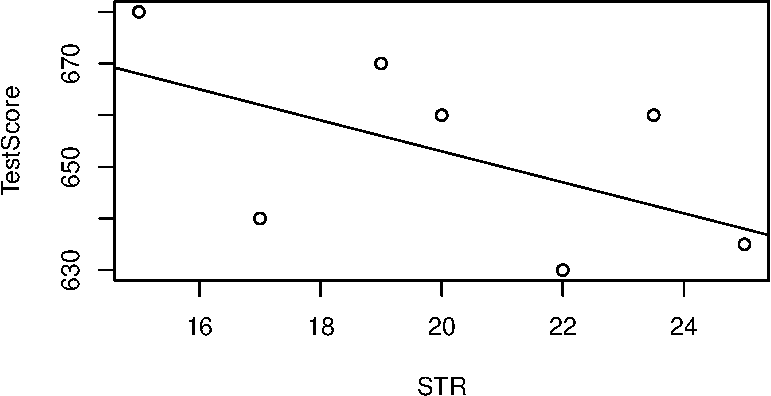
\includegraphics{URFITE_files/figure-latex/unnamed-chunk-139-1} \end{center}

From the plot above we can see that the density estimate has some
similarity to a bivariate normal distribution (see \href{Ch2}{chapter
2}) though it is not very pretty and probably a little rough.
Furthermore, there is correlation between the estimators such that
\(\rho\neq0\) in (2.1). Also, the distribution's shape deviates from the
symmetric bell shape of the bivariate standard normal distribution and
has an eliptical surface area instead.

\begin{Shaded}
\begin{Highlighting}[]
\CommentTok{# estimate correlation between estimators}
\KeywordTok{cor}\NormalTok{(coefs[,}\DecValTok{1}\NormalTok{], coefs[,}\DecValTok{2}\NormalTok{])}
\end{Highlighting}
\end{Shaded}

\begin{verbatim}
## [1] -0.2503028
\end{verbatim}

Where does this correlation come from? Notice that, due to the way we
generated the data, there is correlation between the regressors \(X_1\)
and \(X_2\). Correlation between the regressors in a multiple regression
model always translates to correlation between the estimators (see
Appendix 6.2 of the book). In our case, the positive correlation between
\(X_1\) and \(X_2\) translates to negative correlation between
\(\hat\beta_1\) and \(\hat\beta_2\). To get a better feeling You can
vary the point of view in the subsequent smooth interactive 3D plot of
the same density estimate used for plotting with \texttt{persp}. Here
You can see that the shape of the distribution is somewhat stretched due
to \(\hat\rho=-0.20\) and it is also apparent that both estimators are
unbiased since their joint density seems to be centered close to the
true parameter vector \((\beta_1,\beta_2) = (2.5,3)\).

\hypertarget{14f935020c5ef}{}

\chapter{Hypothesis Tests and Confidence intervals in Multiple
Regression}\label{hypothesis-tests-and-confidence-intervals-in-multiple-regression}

This chapter discusses methods that allow to quantify the sampling
uncertainty inherent to the OLS estimator of coefficients in multiple
regression models. The basis for this are standard errors, hypothesis
tests and confidence intervals which, just as for the simple linear
regression model, can be computed using basic R functions. We will also
tackle the issue of testing joint hypothesis on coefficients of multiple
regression models.

\section{Hypothesis Tests and Confidence Intervals for a Single
Coefficient}\label{hypothesis-tests-and-confidence-intervals-for-a-single-coefficient}

First, we will discuss how to compute standard errors, how to test
hypotheses and how to construct confidence intervals for a single
regression coefficient \(\beta_j\) in a multiple regression model. The
basic idea is summarized in Key Concept 7.1.

Key Concept 7.1

Testing the Hypothesis \(\beta_j = \beta_{j,0}\) Against the Alternative
\(\beta_j \neq \beta_{j,0}\)

\begin{enumerate}
\def\labelenumi{\arabic{enumi}.}
\tightlist
\item
  Compute the standard error of \(\hat{\beta_j}\)
\item
  Compute the \(t\)-statistic,
  \[t = \frac{\hat{\beta}_j - \beta_{j,0}} {SE(\hat{\beta_j})}\]
\item
  Compute the \(p\)-value, \[p\text{-value} = 2 \Phi(-|t^{act}|)\]
\end{enumerate}

where \(t^{act}\) is the value of the \(t\)-statistic actually computed.
Reject the hypothesis at the 5\% significance level if the \(p\)-value
is less than \(0.05\) or, equivalently, if \(|t^{act}| > 1.96\). The
standard error and (typically) the \(t\)-statistic and the corresponding
\(p\)-value for testing \(\beta_j = 0\) are computed automatically by
statistical software, e.g.~by \texttt{summary()}.

It is straightforward to verify that principles of testing single
hypothesis about the significance of coefficients in the multiple
regression model are just as in in the simple regression model.

You can easily see this by inspecting the coefficient summary of the
regression model

\[ TestScore = \beta_0 - \beta_1 \times size - \beta_2 \times english + u \]

already discussed in chapter 6. Let us review this:

\begin{Shaded}
\begin{Highlighting}[]
\NormalTok{model <-}\StringTok{ }\KeywordTok{lm}\NormalTok{(score }\OperatorTok{~}\StringTok{ }\NormalTok{size }\OperatorTok{+}\StringTok{ }\NormalTok{english, }\DataTypeTok{data =}\NormalTok{ CASchools)}
\KeywordTok{summary}\NormalTok{(model)}
\end{Highlighting}
\end{Shaded}

\begin{verbatim}
## 
## Call:
## lm(formula = score ~ size + english, data = CASchools)
## 
## Residuals:
##     Min      1Q  Median      3Q     Max 
## -48.845 -10.240  -0.308   9.815  43.461 
## 
## Coefficients:
##              Estimate Std. Error t value Pr(>|t|)    
## (Intercept) 686.03224    7.41131  92.566  < 2e-16 ***
## size         -1.10130    0.38028  -2.896  0.00398 ** 
## english      -0.64978    0.03934 -16.516  < 2e-16 ***
## ---
## Signif. codes:  0 '***' 0.001 '**' 0.01 '*' 0.05 '.' 0.1 ' ' 1
## 
## Residual standard error: 14.46 on 417 degrees of freedom
## Multiple R-squared:  0.4264, Adjusted R-squared:  0.4237 
## F-statistic:   155 on 2 and 417 DF,  p-value: < 2.2e-16
\end{verbatim}

You may check that these quantities are computed as in the simple
regression model by computing the \(t\)-statistics or \(p\)-values by
hand using the output above and R as a calculator.

For example, using the definition of the \(p\)-value for a two-sided
test as given in Key Concept 7.1, we can confirm the \(p\)-value for a
test of the hypothesis that the coeffiecient \(\beta_0\), that is the
coefficient on \texttt{(intercept)}, is zero to be approximatley zero.

\begin{Shaded}
\begin{Highlighting}[]
\DecValTok{2}\OperatorTok{*}\NormalTok{(}\DecValTok{1}\OperatorTok{-}\KeywordTok{pnorm}\NormalTok{(}\KeywordTok{abs}\NormalTok{(}\FloatTok{92.566}\NormalTok{)))}
\end{Highlighting}
\end{Shaded}

\begin{verbatim}
## [1] 0
\end{verbatim}

Remember that, given a vector of quantiles, \texttt{pnorm()} calculates
associated probabilities for the standard normal distribution by default
which is suitable here since we approximate with the standard normal
distribution.

Key Concept 7.2

Confidence Intervals for a Single Coefficient in Multiple Regression

A \(95\%\) two-sided confidence interval for the coefficient \(\beta_j\)
is an interval that contains the true value of \(\beta_j\) with a
\(95 \%\) probability; that is, it contains the true value of
\(\beta_j\) in \(95 \%\) of all randomly drawn samples. Equivalently, it
is the set of values of \(\beta_j\) that cannot be rejected by a
\(5 \%\) two-sided hypothesis test. When the sample size is large, the
\(95 \%\) confidence interval for \(\beta_j\) is
\[\left[\hat{\beta_j}- 1.96 \times SE(\hat{\beta}_j), \hat{\beta_j} + 1.96 \times SE(\hat{\beta_j})\right].\]

\section{An Application to Test Scores and the Student-Teacher
Ratio}\label{an-application-to-test-scores-and-the-student-teacher-ratio}

Let us take a look at the regression from section 6.3 again.

Computing individual confidence intervals for the coefficients in the
multiple regression model can be done analogously as in the simple
regression model using the function \texttt{confint()}.

\begin{Shaded}
\begin{Highlighting}[]
\NormalTok{model <-}\StringTok{ }\KeywordTok{lm}\NormalTok{(score }\OperatorTok{~}\StringTok{ }\NormalTok{size }\OperatorTok{+}\StringTok{ }\NormalTok{english, }\DataTypeTok{data =}\NormalTok{ CASchools)}
\KeywordTok{confint}\NormalTok{(model)}
\end{Highlighting}
\end{Shaded}

\begin{verbatim}
##                   2.5 %      97.5 %
## (Intercept) 671.4640580 700.6004311
## size         -1.8487969  -0.3537944
## english      -0.7271113  -0.5724424
\end{verbatim}

We note that \(95\%\) confidence intervals for all three coefficients
are computed.

If we want to compute confidence intervals at another level of
\(\alpha=0.1\) say, we just have to set the argument \texttt{level} in
our call of \texttt{confint()} accordingly.

\begin{Shaded}
\begin{Highlighting}[]
\KeywordTok{confint}\NormalTok{(model, }\DataTypeTok{level =} \FloatTok{0.9}\NormalTok{)}
\end{Highlighting}
\end{Shaded}

\begin{verbatim}
##                     5 %        95 %
## (Intercept) 673.8145793 698.2499098
## size         -1.7281904  -0.4744009
## english      -0.7146336  -0.5849200
\end{verbatim}

The output now reports the desired \(90\%\) confidence intervals for all
model coefficients.

Knowing how to use to make inference about the coefficients in multiple
regression models, You can now answer the following question:

Can the null hypothesis that a change in the student-teacher ratio,
\texttt{size}, has no significant influence on test scores,
\texttt{scores}, --- if we control for the percentage of students
learning English in the district, \texttt{english}, --- be rejected at
the \(10\%\) and the \(5\%\) level of significance?

The outputs above tell us that zero is not an element of the computed
confidence intervals for the coefficient of \texttt{size} such that we
can reject the null hypothesis at significance levels of \(5\%\) and
\(10\%\).

Note that rejection at the \(5\%\)-level implies rejection at the
\(10\%\) level (why?).

The same conclusion can be made when beholding the \(p\)-value for
\texttt{size}: \(0.00398 < 0.05 = \alpha\).

The \(95\%\) confidence interval tells us that we can be \(95\%\)
confident that a one-unit decrease in the student-teacher ratio has an
effect on test scores that lies in the interval with a lower bound of
\(-1.8488\) and an upper bound of \(-0.3538\).

\subsection*{Another Augmentation of the
Model}\label{another-augmentation-of-the-model}
\addcontentsline{toc}{subsection}{Another Augmentation of the Model}

What is the average effect on test scores of reducing the
student-teacher ratio when the expenditures per pupil and the percentage
of english learning pupils are held constant?

We can pursue this question by augmenting our model equation by an
additional regressor that is a measure for spendings per pupil. Using
\texttt{?CASchools} we find that \texttt{CASchools} contains the
variable expenditure which provides expenditures per student.

The model we want the estimate now is

\[ TestScore = \beta_0 + \beta_1 \times size + \beta_2 \times english + \beta_3 \times expenditure + u \]

with \(expenditure\) the total amount of expenditures per pupil in the
district (thousands of dollars).

Let us now estimate the model:

\begin{Shaded}
\begin{Highlighting}[]
\CommentTok{# Scale expenditure to thousands of dollars}
\NormalTok{CASchools}\OperatorTok{$}\NormalTok{expenditure <-}\StringTok{ }\NormalTok{CASchools}\OperatorTok{$}\NormalTok{expenditure}\OperatorTok{/}\DecValTok{1000}

\CommentTok{# estimate the model}
\NormalTok{model <-}\StringTok{ }\KeywordTok{lm}\NormalTok{(score }\OperatorTok{~}\StringTok{ }\NormalTok{size }\OperatorTok{+}\StringTok{ }\NormalTok{english }\OperatorTok{+}\StringTok{ }\NormalTok{expenditure, }\DataTypeTok{data =}\NormalTok{ CASchools)}
\KeywordTok{summary}\NormalTok{(model)}
\end{Highlighting}
\end{Shaded}

\begin{verbatim}
## 
## Call:
## lm(formula = score ~ size + english + expenditure, data = CASchools)
## 
## Residuals:
##     Min      1Q  Median      3Q     Max 
## -51.340 -10.111   0.293  10.318  43.181 
## 
## Coefficients:
##              Estimate Std. Error t value Pr(>|t|)    
## (Intercept) 649.57795   15.20572  42.719  < 2e-16 ***
## size         -0.28640    0.48052  -0.596  0.55149    
## english      -0.65602    0.03911 -16.776  < 2e-16 ***
## expenditure   3.86790    1.41212   2.739  0.00643 ** 
## ---
## Signif. codes:  0 '***' 0.001 '**' 0.01 '*' 0.05 '.' 0.1 ' ' 1
## 
## Residual standard error: 14.35 on 416 degrees of freedom
## Multiple R-squared:  0.4366, Adjusted R-squared:  0.4325 
## F-statistic: 107.5 on 3 and 416 DF,  p-value: < 2.2e-16
\end{verbatim}

We see that the estimated effect of a one unit change in the
student-teacher ratio on test scores with expenditures per pupil and the
share of english learning pupils held constant is rather small
(\(-0.29\)). What is more, the coefficient on \(size\) is not
significantly different from zero anymore even at the level of \(10\%\)
since \(p\text{-value}=0.55\). Can You come up with an interpretation
for these findings (see chapter 7.1 of the book)? Mathematically, the
insignificance of \(\beta_1\) could be due to a larger standard error of
\(\hat{\beta}_1\) resulting from adding \(expenditure\) to the model so
that we are estimating the true coefficent on \(size\) less precisely.
This illustrates the issue of strongly correlated regressors (imperfect
multicollinearity). The correlation between \(size\) and
\(expenditures\) can be computed using \texttt{cor()}.

\begin{Shaded}
\begin{Highlighting}[]
\KeywordTok{cor}\NormalTok{(CASchools}\OperatorTok{$}\NormalTok{size, CASchools}\OperatorTok{$}\NormalTok{expenditure)}
\end{Highlighting}
\end{Shaded}

\begin{verbatim}
## [1] -0.6199822
\end{verbatim}

Altogether we conclude that the new model provides no evidence that
changing the student-teacher ratio, e.g.~by hiring new teachers, has any
effect on the test scores while keeping expenditures per student and the
share of english learners constant at the same time.

\section{\texorpdfstring{Joint Hypothesis Testing Using the
\(F\)-Statistic}{Joint Hypothesis Testing Using the F-Statistic}}\label{joint-hypothesis-testing-using-the-f-statistic}

The estimated model is

\[ \widehat{TestScore} = 649.58 -0.29 \times size - 0.66 \times english + 3.87 \times expenditure. \]

Now, can we reject the hypothesis that the coefficient on \(size\) and
and the coefficient on \(expenditure\) are zero? To answer this
question, we have to resort to methods that allow joint hypothesis
testing. A joint hypothesis imposes restrictions on multiple regression
coefficients. This is different from conducting individual \(t\)-tests
where a single resitriction is imposed on a single coefficient. Chapter
7.2 of the book explains why testing the individual coefficients one at
a time is different from testing them jointly.

The homoskedasticity-only \(F\)-Statistic is given by

\[ F = \frac{(SSR_{restricted} - SSR_{unrestricted})/q}{SSR_{unrestricted} / (n-k_{unrestricted}-1)} \]

with \(SSR_{restricted}\) the sum of squared residuals from the
restricted regression, i.e.~the regression where we impose the
restriction. \(SSR_{unrestricted}\) is the sum of squared residuals from
the full model, \(q\) is the number of restriction under the null and
\(k\) is the number of regressors in the unrestricted regression.

Luckily, it is fairly easy to conduct \(F\)-tests in R. We can use the
function \texttt{linearHypothesis()} which is contained in the
\texttt{car} package.

\begin{Shaded}
\begin{Highlighting}[]
\CommentTok{# estimate the multiple regression model}
\NormalTok{model <-}\StringTok{ }\KeywordTok{lm}\NormalTok{(score }\OperatorTok{~}\StringTok{ }\NormalTok{size }\OperatorTok{+}\StringTok{ }\NormalTok{english }\OperatorTok{+}\StringTok{ }\NormalTok{expenditure, }\DataTypeTok{data =}\NormalTok{ CASchools)}

\CommentTok{# execute the function on the model object and provide both linear restrictions }
\CommentTok{# to be tested as strings}
\KeywordTok{linearHypothesis}\NormalTok{(model, }\KeywordTok{c}\NormalTok{(}\StringTok{"size=0"}\NormalTok{, }\StringTok{"expenditure=0"}\NormalTok{))}
\end{Highlighting}
\end{Shaded}

\begin{verbatim}
## Linear hypothesis test
## 
## Hypothesis:
## size = 0
## expenditure = 0
## 
## Model 1: restricted model
## Model 2: score ~ size + english + expenditure
## 
##   Res.Df   RSS Df Sum of Sq      F   Pr(>F)    
## 1    418 89000                                 
## 2    416 85700  2    3300.3 8.0101 0.000386 ***
## ---
## Signif. codes:  0 '***' 0.001 '**' 0.01 '*' 0.05 '.' 0.1 ' ' 1
\end{verbatim}

From the output we can infer that the \(F\)-statistic for this joint
hypothesis test is about \(8.01\) and the corresponding \(p\)-value is
\(0.0004\). Thus we can reject the null hypothesis that both
coefficients are zero at any level of significance commonly used in
practice.

Note:

The standard output of a model summary also reports an \(F\)-statistic
and the corresponding \(p\)-value. The null hypothesis belonging to this
\(F\)-test is that all of the population coefficients in the model
except for the intercept are zero, so the hypotheses pair is

\[H_0: \beta_1=0, \ \beta_2 =0, \ \beta_3 =0 \quad \text{vs.} \quad H_1: \beta_j \neq 0 \ \text{for at least one} \ j=1,2,3.\]

This is also called the ``overall'' regression \(F\)-statistic and the
null hypothesis is obviously different from testing if only \(\beta_1\)
and \(\beta_3\) are zero.

We will now check that the \(F\)-statistic belonging to the \(p\)-value
listed in the model's summary coincides with the result reported by
\texttt{linearHypothesis()}.

\begin{Shaded}
\begin{Highlighting}[]
\CommentTok{# execute the function on the model object and provide the linear restriction }
\CommentTok{# to be tested as strings}
\KeywordTok{linearHypothesis}\NormalTok{(model, }\KeywordTok{c}\NormalTok{(}\StringTok{"size=0"}\NormalTok{,}\StringTok{"english=0"}\NormalTok{,}\StringTok{"expenditure=0"}\NormalTok{))}
\end{Highlighting}
\end{Shaded}

\begin{verbatim}
## Linear hypothesis test
## 
## Hypothesis:
## size = 0
## english = 0
## expenditure = 0
## 
## Model 1: restricted model
## Model 2: score ~ size + english + expenditure
## 
##   Res.Df    RSS Df Sum of Sq      F    Pr(>F)    
## 1    419 152110                                  
## 2    416  85700  3     66410 107.45 < 2.2e-16 ***
## ---
## Signif. codes:  0 '***' 0.001 '**' 0.01 '*' 0.05 '.' 0.1 ' ' 1
\end{verbatim}

\begin{Shaded}
\begin{Highlighting}[]
\CommentTok{# Access the F-statistic from the model's summary}
\KeywordTok{summary}\NormalTok{(model)}\OperatorTok{$}\NormalTok{fstatistic}
\end{Highlighting}
\end{Shaded}

\begin{verbatim}
##    value    numdf    dendf 
## 107.4547   3.0000 416.0000
\end{verbatim}

The test rejects the null hypothesis that the model has no power in
explaining test scores rather clearly.

\section{Confidence Sets for Multiple
Coefficients}\label{confidence-sets-for-multiple-coefficients}

Based on the \(F\)-statistic that we have previously encountered, we can
specify confidence sets. Confidence sets are analogous to confidence
intervals for single coefficients. As such, confidence sets consist of
combinations of coefficients that contain the true combination of
coefficients in, \(95\%\) say, of all cases if we could infinitely draw
random samples, just as in the univariate case. Put differently, a
confidence set is the set of coefficient combinations for which we
cannot reject a joint null hypothesis tested using a \(F\)-test.

If we consider two coefficients, their confidence set is an ellipse
which is centered around the point defined by both coefficient
estimates. Again, there is a very convenient way to plot the confidence
set for two coefficients of model objects, namely the function
\texttt{confidenceEllipse()} which is also coming with the \texttt{car}
package.

In the following, we plot the \(95\%\) confidence ellipse for the
coefficients on \texttt{size} and \texttt{expenditure} from the
regression conducted above. By specifying the additional argument
\texttt{fill}, the confidence set is colored which gives us a better
impression which set of coefficients is meant.

\begin{Shaded}
\begin{Highlighting}[]
\CommentTok{# Draw the 95% confidence set for coefficients on size and expenditure}
\KeywordTok{confidenceEllipse}\NormalTok{(model, }
                  \DataTypeTok{fill =}\NormalTok{ T, }
                  \DataTypeTok{which.coef =} \KeywordTok{c}\NormalTok{(}\StringTok{"size"}\NormalTok{,}\StringTok{"expenditure"}\NormalTok{),}
                  \DataTypeTok{main =} \StringTok{"95% Confidence Set"}
\NormalTok{                  )}
\end{Highlighting}
\end{Shaded}

\begin{center}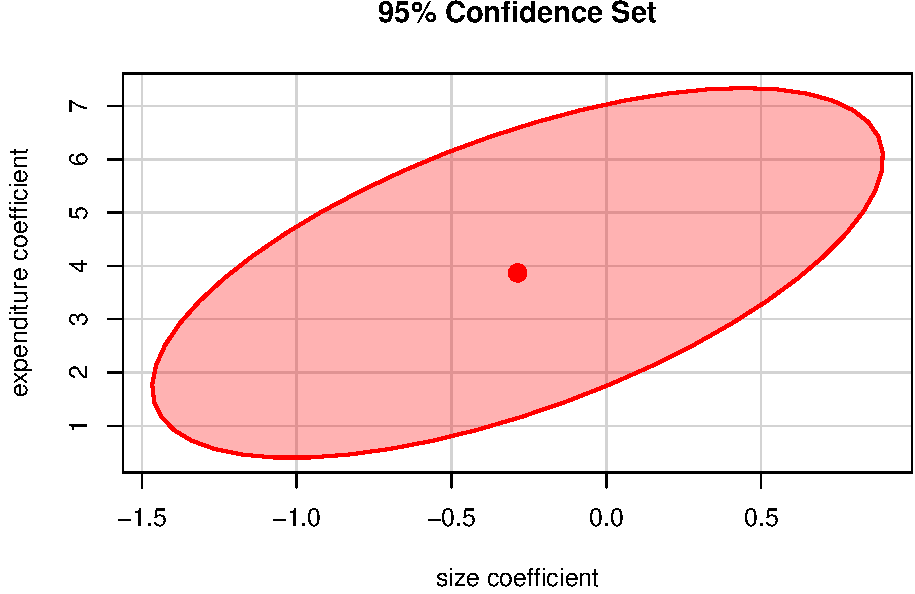
\includegraphics{URFITE_files/figure-latex/unnamed-chunk-150-1} \end{center}

We see that the ellipse is centered around \((-0.29, 3.87)\) i.e.~the
pair of coefficients estimates on \(size\) and \(expenditure\). What is
more, \((0,0)\) is not element of the \(95\%\) confidence set so that we
can reject \(H_0: \beta_1 = 0, \ \beta_3 = 0\).

\section{Model Specification for Multiple
Regression}\label{model-specification-for-multiple-regression}

Choosing a regression specifaction i.e.~selecting the variables to be
included in a regression model can be quite cumbersome. However, there
are some guidelines how to do this. The goal is clear: obtaining an
unbiased estimation of the causal effect of interest. As a starting
point, one should think about omitted variables, that is to avoid a
possible estimation bias by using suitable control variables (omitted
variables bias in the context of multiple regression is explained in Key
Concept 7.3). A second step could be to compare different regression
model specifications by measures of fit. However, as we shall see one
should not rely solely on \(\overline{R^2}\).

Key Concept 7.3

Omitted Variable Bias in Multiple Regression

Omitted variable bias is the bias in the OLS estimator that arises when
one or more included regressors are correlated with an omitted variable.
For omitted variable bias to arise, two things must be true:

\begin{enumerate}
\def\labelenumi{\arabic{enumi}.}
\tightlist
\item
  At least one of the included regressors must be correlated with the
  omitted variable.
\item
  The omitted variable must be a determinant of the dependent variable,
  \(Y\).
\end{enumerate}

We will now discuss an example were we face a potential omitted variable
bias in a multiple regression model:

Consider again the estimated regression equation

\[ \widehat{TestScore} = \underset{(8.7)}{686.0} - \underset{(0.43)}{1.10} \times size - \underset{(0.031)}{0.650} \times english. \]

We are interested in estimated the causal effect of class size on test
score. In this estimation, there might be a bias due to omitting
``outside learning opportunities'' from our regression sice a measure
like this could be a determinant of the students test scores and could
also be correlated with both regressors already included in the model
(so that both conditions of Key Concept 7.3 are fulfilled). ``outside
learning opportunities'' is a complicated concept that is difficult to
quantify. A surrogate we can consider instead is the students' economic
backgroud which should be strongly related to the outside learning
opportunities: think of wealthy parents that are able to provide time
and/or money for private tuition of there children. We thus augment the
model with the variable \texttt{lunch}, the percentage of students that
qualify for a free or subsidized lunch in school due to family incomes
below a certain threshold, and estimate the model again.

\begin{Shaded}
\begin{Highlighting}[]
\CommentTok{# estimate the model and print summary to console}
\NormalTok{model <-}\StringTok{ }\KeywordTok{lm}\NormalTok{(score }\OperatorTok{~}\StringTok{ }\NormalTok{size }\OperatorTok{+}\StringTok{ }\NormalTok{english }\OperatorTok{+}\StringTok{ }\NormalTok{lunch, }\DataTypeTok{data =}\NormalTok{ CASchools)}
\KeywordTok{summary}\NormalTok{(model)}
\end{Highlighting}
\end{Shaded}

\begin{verbatim}
## 
## Call:
## lm(formula = score ~ size + english + lunch, data = CASchools)
## 
## Residuals:
##     Min      1Q  Median      3Q     Max 
## -32.849  -5.151  -0.308   5.243  31.501 
## 
## Coefficients:
##              Estimate Std. Error t value Pr(>|t|)    
## (Intercept) 700.14996    4.68569 149.423  < 2e-16 ***
## size         -0.99831    0.23875  -4.181 3.54e-05 ***
## english      -0.12157    0.03232  -3.762 0.000193 ***
## lunch        -0.54735    0.02160 -25.341  < 2e-16 ***
## ---
## Signif. codes:  0 '***' 0.001 '**' 0.01 '*' 0.05 '.' 0.1 ' ' 1
## 
## Residual standard error: 9.08 on 416 degrees of freedom
## Multiple R-squared:  0.7745, Adjusted R-squared:  0.7729 
## F-statistic: 476.3 on 3 and 416 DF,  p-value: < 2.2e-16
\end{verbatim}

Thus, the estimated regression line is

\[ \widehat{TestScore} = \underset{(4.7)}{700.15} - \underset{(0.24)}{1.00} \times size - \underset{(0.032)}{0.12} \times english + \underset{(0.022)}{0.55} \times lunch. \]

We observe no substantial changes in the conclusion about the effect of
\texttt{size}: the coefficient changes by only \(0.1\) and keeps its
significance.

Although the difference in estimated coefficients is not big in this
case, it might be a good idea to keep \texttt{lunch} in the model to
make the assumption of conditional mean independence more credible (see
chapter 7.5 of the book).

\subsection*{Model Specification in Theory and in
Practice}\label{model-specification-in-theory-and-in-practice}
\addcontentsline{toc}{subsection}{Model Specification in Theory and in
Practice}

Key Concept 7.4

\(R^2\) and \(\overline{R^2}\): What They Tell You --- and What They
Don't

The \(R^2\) and \(\overline{R^2}\) tell you whether the regressors are
good at predicting, or ``explaining'' the values of the independent
variable in the sample of data at hand. if the \(R^2\) (or
\(\overline{R^2}\)) is nearly \(1\), then the regressors produce good
prediction of the dependent variable in that sample, in the sense that
the variance of OLS residuals is small compared to the variance of the
dependent variable. If the \(R^2\) (or \(\overline{R^2}\)) is nearly
\(0\), the opposite is true.

The \(R^2\) and \(\overline{R^2}\) do not tell you whether:

\begin{enumerate}
\def\labelenumi{\arabic{enumi}.}
\tightlist
\item
  An included variable is statistically significant.
\item
  The regressors are true cause of the movements in the dependent
  variable
\item
  There is omitted variable bias, or
\item
  You have chosen the most appropriate set of regressors.
\end{enumerate}

Key Concept 7.4 names some common pitfalls when using \(R^2\) and
\(\overline{R^2}\) to evaluate the predictive ability of regression
models.

For example, think of regressing \(TestScore\) on \(PLS\) which measures
the available parking lot space in thousand square feet. You are likely
to observe a significant coefficient of reasonable magnitude and
moderate to high values for \(R^2\) and \(\overline{R^2}\). The reason
for this is that parking lot space is correlated with many determinants
of the test score like location, class size, financial endowment and so
on. Although we do not have observations on \(PLS\), we can use R to
generate some relatively realistic data.

\begin{Shaded}
\begin{Highlighting}[]
\CommentTok{# Generate observations for parking lot space}
\NormalTok{CASchools}\OperatorTok{$}\NormalTok{PLS <-}\StringTok{ }\DecValTok{5} \OperatorTok{+}\StringTok{ }\FloatTok{0.6}\OperatorTok{*}\NormalTok{CASchools}\OperatorTok{$}\NormalTok{expenditure }\OperatorTok{+}\StringTok{ }\FloatTok{0.6}\OperatorTok{*}\NormalTok{CASchools}\OperatorTok{$}\NormalTok{income }\OperatorTok{+}\StringTok{ }\NormalTok{CASchools}\OperatorTok{$}\NormalTok{size}\OperatorTok{/}\DecValTok{100} \OperatorTok{+}\StringTok{ }\KeywordTok{rnorm}\NormalTok{(}\KeywordTok{nrow}\NormalTok{(CASchools), }\DataTypeTok{sd =} \DecValTok{1}\NormalTok{)}

\CommentTok{# plot parking lot space against test score}
\KeywordTok{plot}\NormalTok{(CASchools}\OperatorTok{$}\NormalTok{PLS, }
\NormalTok{     CASchools}\OperatorTok{$}\NormalTok{score,}
     \DataTypeTok{xlab =} \StringTok{"Parking Lot Space"}\NormalTok{,}
     \DataTypeTok{ylab =} \StringTok{"Test Score"}\NormalTok{,}
     \DataTypeTok{pch =} \DecValTok{20}\NormalTok{,}
     \DataTypeTok{col =} \StringTok{"steelblue"}
\NormalTok{     )}
\end{Highlighting}
\end{Shaded}

\begin{center}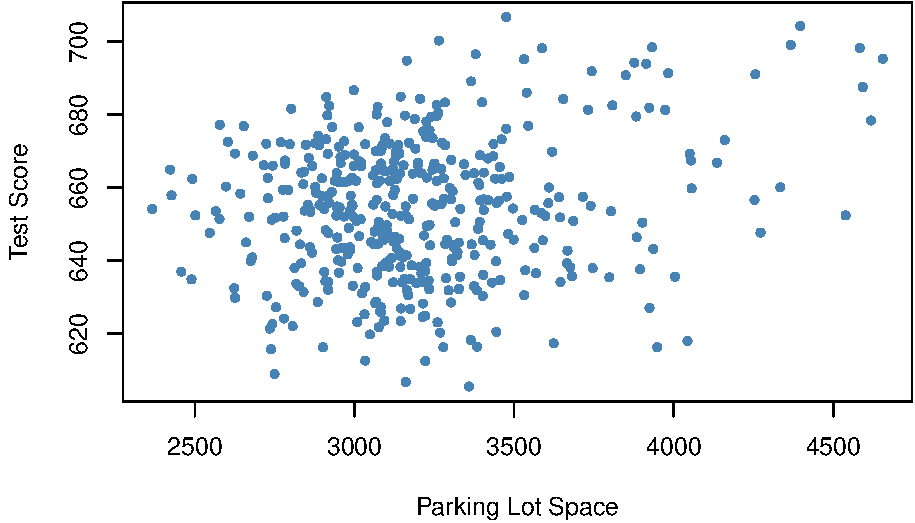
\includegraphics{URFITE_files/figure-latex/unnamed-chunk-152-1} \end{center}

\begin{Shaded}
\begin{Highlighting}[]
\CommentTok{# regress test score on PLS}
\KeywordTok{summary}\NormalTok{(}\KeywordTok{lm}\NormalTok{(score }\OperatorTok{~}\StringTok{ }\NormalTok{PLS, }\DataTypeTok{data =}\NormalTok{ CASchools))}
\end{Highlighting}
\end{Shaded}

\begin{verbatim}
## 
## Call:
## lm(formula = score ~ PLS, data = CASchools)
## 
## Residuals:
##    Min     1Q Median     3Q    Max 
## -50.16 -14.25   0.65  13.56  49.88 
## 
## Coefficients:
##              Estimate Std. Error t value Pr(>|t|)    
## (Intercept) 6.224e+02  7.715e+00  80.679  < 2e-16 ***
## PLS         9.915e-03  2.393e-03   4.144 4.13e-05 ***
## ---
## Signif. codes:  0 '***' 0.001 '**' 0.01 '*' 0.05 '.' 0.1 ' ' 1
## 
## Residual standard error: 18.7 on 418 degrees of freedom
## Multiple R-squared:  0.03946,    Adjusted R-squared:  0.03717 
## F-statistic: 17.17 on 1 and 418 DF,  p-value: 4.131e-05
\end{verbatim}

\(PLS\) is generated as a linear function of \(expenditure\),
\(income\), \(size\) and random disturbances. Therefore the data suggest
that there is some postive relationship between parking lot space and
test score. In fact, when estimating the model

\begin{align}
\widehat{TestScore} = \beta_0 + \beta_1 \times PLS + u \label{eq:plsmod} 
\end{align}

using \texttt{lm()} we find that the coefficient on \(PLS\) is positive
and significantly different from zero. Also \(R^2\) and
\(\overline{R^2}\) are about \(0.47\) which is a lot more than the
roughly \(0.05\) observed when regressing test score on class size only.

This suggests that increasing the parking lot space boosts a school's
test scores and that model \eqref{eq:plsmod} does even better in
explaining heterogeneity in the dependent variable than a model with
\(size\) as the only regressor. Keeping in mind how \(PLS\) is
constructed this comes of no surprise. It is evident that the high
\(R^2\) cannot be used to the conclude that the estimated relation
between parking lot space and test scores is causal: the (relatively)
high \(R^2\) is due to correlation between \(PLS\) and other
determinantes and/or control variables. Increasing parking lot space is
not an appropriate measure to generate more learning success!

\section{Analysis of the Test Score Data
Set}\label{analysis-of-the-test-score-data-set}

Chapter 6 and some of the previous sections have stressed that it is
important to include control variables in regression models if it is
plausible that there are omitted factors that cannot be measured
directly. Recall that in our example of test scores, we are interested
in estimating the causal effect of a change in the student-teacher ratio
on test scores. In what follows, we will provide an example how to use
multiple regression models in order to alleviate omitted variable bias
and we will demonstrate how to report results using R.

So far we have considered two variables that control for unobservable
student characteristics which correlate with the student-teacher ratio
and are assumed to have an impact on test scores:

\begin{itemize}
\item
  \(english\), the percentage of english learning students
\item
  \(lunch\), the share of students that qualify for a subsidized or even
  a free lunch at school
\end{itemize}

Another new variable provided with \texttt{CASchools} is \(calworks\),
the percentage of students that qualify for the CalWorks income
assistance programm. Students eligible for CalWorks live in families
with a total income below the threshold for the subsidized lunch
programm so both variables are indicators for the share of economically
disadvantaged children. Using R we can confirm that both indicators are
highly correlated:

\begin{Shaded}
\begin{Highlighting}[]
\CommentTok{# estimate correlation between calworks and lunch}
\KeywordTok{cor}\NormalTok{(CASchools}\OperatorTok{$}\NormalTok{calworks, CASchools}\OperatorTok{$}\NormalTok{lunch)}
\end{Highlighting}
\end{Shaded}

\begin{verbatim}
## [1] 0.7394218
\end{verbatim}

There is no unabigious way to proceed when deciding which variable to
use. In any case it is not a good idea to use both variables as
regressors having in mind consequences of colinearity. Therefore, we
will also consider alternative model specifications.

For a start, we plot student characteristics against test scores.

\begin{Shaded}
\begin{Highlighting}[]
\KeywordTok{par}\NormalTok{(}\DataTypeTok{mfrow =} \KeywordTok{c}\NormalTok{(}\DecValTok{1}\NormalTok{,}\DecValTok{3}\NormalTok{))}

\NormalTok{m <-}\StringTok{ }\KeywordTok{rbind}\NormalTok{(}\KeywordTok{c}\NormalTok{(}\DecValTok{1}\NormalTok{, }\DecValTok{2}\NormalTok{), }\KeywordTok{c}\NormalTok{(}\DecValTok{3}\NormalTok{, }\DecValTok{0}\NormalTok{))}
\KeywordTok{layout}\NormalTok{(m)}

\KeywordTok{plot}\NormalTok{(score }\OperatorTok{~}\StringTok{ }\NormalTok{english, }
     \DataTypeTok{data =}\NormalTok{ CASchools, }
     \DataTypeTok{col =} \StringTok{"steelblue"}\NormalTok{, }
     \DataTypeTok{pch =} \DecValTok{20}\NormalTok{, }
     \DataTypeTok{xlim =} \KeywordTok{c}\NormalTok{(}\DecValTok{0}\NormalTok{,}\DecValTok{100}\NormalTok{), }
     \DataTypeTok{main =} \StringTok{"Percentage of English language learners"}\NormalTok{)}

\KeywordTok{plot}\NormalTok{(score }\OperatorTok{~}\StringTok{ }\NormalTok{lunch, }
     \DataTypeTok{data =}\NormalTok{ CASchools, }
     \DataTypeTok{col =} \StringTok{"steelblue"}\NormalTok{, }
     \DataTypeTok{pch =} \DecValTok{20}\NormalTok{,}
     \DataTypeTok{main =} \StringTok{"Percentage qualifying for reduced price lunch"}\NormalTok{)}

\KeywordTok{plot}\NormalTok{(score }\OperatorTok{~}\StringTok{ }\NormalTok{calworks, }
     \DataTypeTok{data =}\NormalTok{ CASchools, }
     \DataTypeTok{col =} \StringTok{"steelblue"}\NormalTok{, }
     \DataTypeTok{pch =} \DecValTok{20}\NormalTok{, }
     \DataTypeTok{xlim =} \KeywordTok{c}\NormalTok{(}\DecValTok{0}\NormalTok{,}\DecValTok{100}\NormalTok{), }
     \DataTypeTok{main =} \StringTok{"Percentage qualifying for income assistance"}\NormalTok{)}
\end{Highlighting}
\end{Shaded}

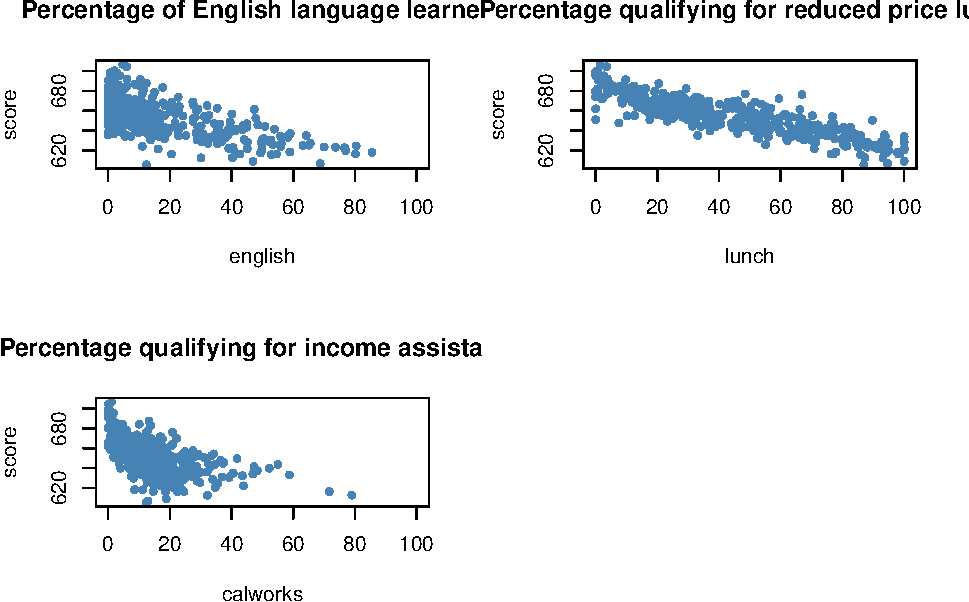
\includegraphics{URFITE_files/figure-latex/unnamed-chunk-154-1.pdf}

We see that all relationships are negative. We can use R to estimate the
correlation coefficients.

\begin{Shaded}
\begin{Highlighting}[]
\CommentTok{# estimate correlation between student characteristics and test scores}
\KeywordTok{cor}\NormalTok{(CASchools}\OperatorTok{$}\NormalTok{score, CASchools}\OperatorTok{$}\NormalTok{english)}
\end{Highlighting}
\end{Shaded}

\begin{verbatim}
## [1] -0.6441238
\end{verbatim}

\begin{Shaded}
\begin{Highlighting}[]
\KeywordTok{cor}\NormalTok{(CASchools}\OperatorTok{$}\NormalTok{score, CASchools}\OperatorTok{$}\NormalTok{lunch)}
\end{Highlighting}
\end{Shaded}

\begin{verbatim}
## [1] -0.868772
\end{verbatim}

\begin{Shaded}
\begin{Highlighting}[]
\KeywordTok{cor}\NormalTok{(CASchools}\OperatorTok{$}\NormalTok{score, CASchools}\OperatorTok{$}\NormalTok{calworks)}
\end{Highlighting}
\end{Shaded}

\begin{verbatim}
## [1] -0.6268533
\end{verbatim}

We will consider \(5\) different model equations:

\begin{align*}
  (I) \quad \widehat{TestScore} =& \, \beta_0 + \beta_1 \times size + u \\
  (II) \quad \widehat{TestScore} =& \, \beta_0 + \beta_1 \times size + \beta_2 \times english + u \\
  (III) \quad \widehat{TestScore} =& \, \beta_0 + \beta_1 \times size + \beta_2 \times english + \beta_3 \times lunch + u \\
  (IV) \quad \widehat{TestScore} =& \, \beta_0 + \beta_1 \times size + \beta_2 \times english + \beta_4 \times calworks + u \\
  (V) \quad \widehat{TestScore} =& \, \beta_0 + \beta_1 \times size + \beta_2 \times english + \beta_3 \times lunch + \beta_4 \times calworks + u
\end{align*}

The best way to communicate regression results is in a table. The
\texttt{stargazer} package is very convenient for this purpose. It
provides a function that generates professionally looking HTML and LATEX
tables that satisfy scienctific standards. One simply has to provide one
or multiple object(s) of class \texttt{lm} and the rest is done by the
function \texttt{stargazer()}.

\begin{Shaded}
\begin{Highlighting}[]
\CommentTok{# load the stargazer library}
\KeywordTok{library}\NormalTok{(stargazer)}

\CommentTok{# estimate different model specifications}
\NormalTok{spec1 <-}\StringTok{ }\KeywordTok{lm}\NormalTok{(score }\OperatorTok{~}\StringTok{ }\NormalTok{size , }\DataTypeTok{data =}\NormalTok{ CASchools)}
\NormalTok{spec2 <-}\StringTok{ }\KeywordTok{lm}\NormalTok{(score }\OperatorTok{~}\StringTok{ }\NormalTok{size }\OperatorTok{+}\StringTok{ }\NormalTok{english, }\DataTypeTok{data =}\NormalTok{ CASchools)}
\NormalTok{spec3 <-}\StringTok{ }\KeywordTok{lm}\NormalTok{(score }\OperatorTok{~}\StringTok{ }\NormalTok{size }\OperatorTok{+}\StringTok{ }\NormalTok{english }\OperatorTok{+}\StringTok{ }\NormalTok{lunch, }\DataTypeTok{data =}\NormalTok{ CASchools)}
\NormalTok{spec4 <-}\StringTok{ }\KeywordTok{lm}\NormalTok{(score }\OperatorTok{~}\StringTok{ }\NormalTok{size }\OperatorTok{+}\StringTok{ }\NormalTok{english }\OperatorTok{+}\StringTok{ }\NormalTok{calworks, }\DataTypeTok{data =}\NormalTok{ CASchools)}
\NormalTok{spec5 <-}\StringTok{ }\KeywordTok{lm}\NormalTok{(score }\OperatorTok{~}\StringTok{ }\NormalTok{size }\OperatorTok{+}\StringTok{ }\NormalTok{english }\OperatorTok{+}\StringTok{ }\NormalTok{lunch }\OperatorTok{+}\StringTok{ }\NormalTok{calworks, }\DataTypeTok{data =}\NormalTok{ CASchools)}

\CommentTok{# generate a Latex table using stargazer}
\KeywordTok{stargazer}\NormalTok{(spec1, spec2, spec3, spec4, spec5, }
          \DataTypeTok{column.labels =} \KeywordTok{c}\NormalTok{(}\StringTok{"(I)"}\NormalTok{, }\StringTok{"(II)"}\NormalTok{, }\StringTok{"(III)"}\NormalTok{, }\StringTok{"(IV)"}\NormalTok{, }\StringTok{"(V)"}\NormalTok{)}
\NormalTok{          )}
\end{Highlighting}
\end{Shaded}

Dependent variable:

score

(I)

(II)

(III)

(IV)

(V)

spec1

spec2

spec3

spec4

spec5

size

-2.280***

-1.101***

-0.998***

-1.308***

-1.014***

(0.480)

(0.380)

(0.239)

(0.307)

(0.240)

english

-0.650***

-0.122***

-0.488***

-0.130***

(0.039)

(0.032)

(0.033)

(0.034)

lunch

-0.547***

-0.529***

(0.022)

(0.032)

calworks

-0.790***

-0.048

(0.053)

(0.061)

Constant

698.933***

686.032***

700.150***

697.999***

700.392***

(9.467)

(7.411)

(4.686)

(6.024)

(4.698)

Observations

420

420

420

420

420

R2

0.051

0.426

0.775

0.629

0.775

Adjusted R2

0.049

0.424

0.773

0.626

0.773

Residual Std. Error

18.581 (df = 418)

14.464 (df = 417)

9.080 (df = 416)

11.654 (df = 416)

9.084 (df = 415)

F Statistic

22.575*** (df = 1; 418)

155.014*** (df = 2; 417)

476.306*** (df = 3; 416)

234.638*** (df = 3; 416)

357.054*** (df = 4; 415)

Note:

\emph{p\textless{}0.1; \textbf{p\textless{}0.05; }}p\textless{}0.01

The table states that \(scores\) is the dependent variable and that we
consider \(5\) models. We see that the coloumns of Table 7.1 contain all
the information provided by \texttt{summary()} for the regression models
\texttt{spec1} to \texttt{spec5}: the coefficient section of the table
presents coefficients estimates equipped with signifiance codes
(asterisks) and standard errors in parantheses below. Although there a
no \(t\)-statistics, it is straightforward for the reader to compute
them simply by dividing a coefficient estimate by the correspondung
standard error. In the botton of the table we find summary statistics
for each model and a legend. For an in-depth discussion of the tabular
presentation of regression results, see chapter 7.6 of the book.

What can we conclude from the model comparison?

\begin{enumerate}
\def\labelenumi{\arabic{enumi}.}
\item
  We see that adding control variables roughly halves the coefficient on
  \texttt{size}. Also the coefficient is not very sensitive to the set
  of control variables used. The conclusion is that decreasing the
  student-teacher ratio ceteris paribus by one unit leads to an
  estimated average increase in test scores of about \(1\) point.
\item
  Adding student characteristics as controls boosts \(R^2\) and
  \(\overline{R^2}\) from \(0.049\) (\texttt{spec1}) up to \(0.773\)
  (\texttt{spec3} and \texttt{spec5}), so we can consider these
  variables as suitable predictors for test scores. Morever, the
  estimated coefficients on all control variables are consistent with
  the impressions gained from figure 7.2.
\item
  We see that the control variables are not always individually
  statistically significant: for example in \texttt{spec5} we see that
  the coefficient on \(calworks\) is not significantly different from
  zero at the level of \(5\%\) since
  \(\lvert-0.048/0.061\rvert=0.79 < 1.64\). We also observe that the
  effect on the estimate (and its standard error) of the coefficient on
  \(size\) of adding \(calworks\) to the base specification
  \texttt{spec3} is negligible. We can therefore consider
  \texttt{calworks} as a redundant control variable in this setting.
\end{enumerate}

\chapter{Nonlinear Regression
Functions}\label{nonlinear-regression-functions}

Until now we assumed the regression function to be linear, i.e.~we have
treated the slope of the regression function as a constant. This implies
that the effect on \(Y\) of a one unit change in \(X\) does not depend
on the level of \(X\). If however the effect of a change in \(X\) on
\(Y\) does depend on the value of \(X\), we have to use a nonlinear
regression function.

\section{A General Strategy for Modeling Nonlinear Regression
Functions}\label{a-general-strategy-for-modeling-nonlinear-regression-functions}

Let us have a look at an example where in fact using a nonlinear
regression function is better suited for estimation of the population
relationship between the regressor, \(X\), and the regressand, \(Y\):
the relationship between the income of schooling districts and their
test scores.

\begin{Shaded}
\begin{Highlighting}[]
\CommentTok{#Prepare the data}
\KeywordTok{library}\NormalTok{(AER)                                                     }
\KeywordTok{data}\NormalTok{(CASchools)}
\NormalTok{CASchools}\OperatorTok{$}\NormalTok{size <-}\StringTok{ }\NormalTok{CASchools}\OperatorTok{$}\NormalTok{students}\OperatorTok{/}\NormalTok{CASchools}\OperatorTok{$}\NormalTok{teachers}
\NormalTok{CASchools}\OperatorTok{$}\NormalTok{score <-}\StringTok{ }\NormalTok{(CASchools}\OperatorTok{$}\NormalTok{read }\OperatorTok{+}\StringTok{ }\NormalTok{CASchools}\OperatorTok{$}\NormalTok{math)}\OperatorTok{/}\DecValTok{2}       
\end{Highlighting}
\end{Shaded}

We start our analysis by computing the correlation between the two
variables.

\begin{Shaded}
\begin{Highlighting}[]
\KeywordTok{cor}\NormalTok{(CASchools}\OperatorTok{$}\NormalTok{income, CASchools}\OperatorTok{$}\NormalTok{score)}
\end{Highlighting}
\end{Shaded}

\begin{verbatim}
## [1] 0.7124308
\end{verbatim}

The correlation coefficient is about \(0.71\). This means that income
and test scores are positively correlated. In other words, children
whose parents have an above average income tend to achieve above average
test scores. Can we use the correlation coefficient to assess whether a
linear regression model does fit the data adequately? To answer this
question we visualize the data and add a linear regression line to the
plot.

\begin{Shaded}
\begin{Highlighting}[]
\CommentTok{#Fit linear model}
\NormalTok{linear_model<-}\StringTok{ }\KeywordTok{lm}\NormalTok{(score }\OperatorTok{~}\StringTok{ }\NormalTok{income, }\DataTypeTok{data =}\NormalTok{ CASchools)}

\CommentTok{# Plot observations}
\KeywordTok{plot}\NormalTok{(CASchools}\OperatorTok{$}\NormalTok{income, CASchools}\OperatorTok{$}\NormalTok{score,}
     \DataTypeTok{col =} \StringTok{"steelblue"}\NormalTok{,}
     \DataTypeTok{pch =} \DecValTok{20}\NormalTok{,}
     \DataTypeTok{xlab =} \StringTok{"District Income (thousands of dollars)"}\NormalTok{, }
     \DataTypeTok{ylab =} \StringTok{"Test Score"}\NormalTok{,}
     \DataTypeTok{main =} \StringTok{"Test Score vs. District Income and a Linear OLS Regression Function"}\NormalTok{)}

\CommentTok{# Add the regression line to the plot}
\KeywordTok{abline}\NormalTok{(linear_model, }\DataTypeTok{col=}\StringTok{"red"}\NormalTok{, }\DataTypeTok{lwd=}\DecValTok{2}\NormalTok{)}
\end{Highlighting}
\end{Shaded}

\begin{center}\includegraphics{URFITE_files/figure-latex/unnamed-chunk-159-1} \end{center}

As Stock and Watson point out, the linear regression line seems to
overestimate the true relationship when income is very high or very low
and underestimates it in the midrange.

Fortunately, usage of the OLS is not restricted to linear functions of
the regressors. Thus we can for example model test scores as a function
of income and the square of income. The corresponding regression model
is

\[TestScore_i = \beta_0 + \beta_1 Income_i + \beta_2 Income_i^2 + u_i.\]

This equation is called the \emph{quadratic regression model}. Note,
that \(Income^2\) is treated as an additional explanatory variable.
Hence, the quadratic model is a special case of a multivariate
regression model. When fitting the model with \texttt{lm()} we have to
use the \texttt{\^{}} operator in conjunction with the function
\texttt{I()} to add the quadratic term as an additional regressor to the
\texttt{formula} argument.

\begin{Shaded}
\begin{Highlighting}[]
\CommentTok{# Fit the quadratic Model}
\NormalTok{quadratic_model <-}\StringTok{ }\KeywordTok{lm}\NormalTok{(score }\OperatorTok{~}\StringTok{ }\NormalTok{income }\OperatorTok{+}\StringTok{ }\KeywordTok{I}\NormalTok{(income}\OperatorTok{^}\DecValTok{2}\NormalTok{), }\DataTypeTok{data =}\NormalTok{ CASchools)}

\CommentTok{# Generate model summary}
\KeywordTok{summary}\NormalTok{(quadratic_model)}
\end{Highlighting}
\end{Shaded}

\begin{verbatim}
## 
## Call:
## lm(formula = score ~ income + I(income^2), data = CASchools)
## 
## Residuals:
##     Min      1Q  Median      3Q     Max 
## -44.416  -9.048   0.440   8.347  31.639 
## 
## Coefficients:
##              Estimate Std. Error t value Pr(>|t|)    
## (Intercept) 607.30174    3.04622 199.362  < 2e-16 ***
## income        3.85099    0.30426  12.657  < 2e-16 ***
## I(income^2)  -0.04231    0.00626  -6.758 4.71e-11 ***
## ---
## Signif. codes:  0 '***' 0.001 '**' 0.01 '*' 0.05 '.' 0.1 ' ' 1
## 
## Residual standard error: 12.72 on 417 degrees of freedom
## Multiple R-squared:  0.5562, Adjusted R-squared:  0.554 
## F-statistic: 261.3 on 2 and 417 DF,  p-value: < 2.2e-16
\end{verbatim}

The output tells us that the estimated model equation is

\[ \widehat{TestScore}_i = \underset{(3.05)}{607.3} + \underset{(0.30)}{3.85} \times Income_i - \underset{(0.01)}{0.0423} \times Income_i^2. \]

Notice that this estimated model equation allows us to test the
hypothesis that the relationship between test scores and district income
is linear against the alternative hypothesis that it is nonlinear. This
corresponds to testing

\[ H_0: \beta_2 = 0 \ \ \text{vs.} \ \  H_1: \beta_2\neq0,\]

since \(\beta_2=0\) corresponds to a simple linear equation and and
\(\beta_2\neq0\) implies a quadratic relationship. We find that
\(t=(\hat\beta_2 - 0)/SE(\hat\beta_2) = -0.0423/0.01 = -4.23\) so the
null is rejected at any common level of significance and we conclude
that the relationship is nonlinear. This is consistent with our informal
inspection of the plotted data.

We can now draw the same scatterplot as for the linear model and add the
regression line for the quadratic model. Because \texttt{abline()} can
only draw straight lines, it cannot be used for this task. A function
which can be used to draw lines without being restricted to straight
lines is \texttt{lines()}, see \texttt{?lines}. The most basic call of
\texttt{lines()} is \texttt{lines(x\_values,\ y\_values)} where
\texttt{x\_values} and \texttt{y\_values} are vectors of the same length
that provide coordinates of the points to be sequentially connected by a
line. This makes it necessary to sort the coordinate pairs according to
the X-values. Otherwise You will not get the desired result! In this
example we use the function \texttt{order()} to sort the fitted values
of \(TestScore\) according to the observations for \(income\).

\begin{Shaded}
\begin{Highlighting}[]
\CommentTok{# Scatterplot of observatuib for income and TestScore}
\KeywordTok{plot}\NormalTok{(CASchools}\OperatorTok{$}\NormalTok{income, CASchools}\OperatorTok{$}\NormalTok{score,}
     \DataTypeTok{col  =} \StringTok{"steelblue"}\NormalTok{,}
     \DataTypeTok{pch =} \DecValTok{20}\NormalTok{,}
     \DataTypeTok{xlab =} \StringTok{"District Income (thousands of dollars)"}\NormalTok{,}
     \DataTypeTok{ylab =} \StringTok{"Test Score"}\NormalTok{,}
     \DataTypeTok{main =} \StringTok{"Linear and Quadratic OLS Regression Functions"}\NormalTok{)}

\CommentTok{#Add linear function to the plot}
\KeywordTok{abline}\NormalTok{(linear_model , }\DataTypeTok{col=}\StringTok{"black"}\NormalTok{, }\DataTypeTok{lwd=}\DecValTok{2}\NormalTok{)}

\CommentTok{#Add quatratic function to the plot}
\NormalTok{order_id <-}\StringTok{ }\KeywordTok{order}\NormalTok{(CASchools}\OperatorTok{$}\NormalTok{income)}

\KeywordTok{lines}\NormalTok{(}\DataTypeTok{x =}\NormalTok{ CASchools}\OperatorTok{$}\NormalTok{income[order_id], }
      \DataTypeTok{y =} \KeywordTok{fitted}\NormalTok{(quadratic_model)[order_id],}
      \DataTypeTok{col=}\StringTok{"red"}\NormalTok{, }
      \DataTypeTok{lwd=}\DecValTok{2}\NormalTok{) }
\end{Highlighting}
\end{Shaded}

\begin{center}\includegraphics{URFITE_files/figure-latex/unnamed-chunk-161-1} \end{center}

We see that the quadratic model does much better in fitting the data
than the linear model.

\section{Nonlinear Functions of a Single Independent
Variable}\label{nonlinear-functions-of-a-single-independent-variable}

\subsection*{Polynomials}\label{polynomials}
\addcontentsline{toc}{subsection}{Polynomials}

The approach used to obtain a quadratic model can be generalized to
polynomial models of arbitrary order \(r\).
\[Y_i = \beta_0 + \beta_1 X_i + \beta_2 X_i^2 + \ldots + \beta_r X_i^r + u_i\]

A cubic model (\(r=3\)) for instance can be estimated in the same way as
the quadratic model --- we just have to add \texttt{I(income\^{}3)} to
the \texttt{formula} argument in our call of \texttt{lm()}.

\begin{Shaded}
\begin{Highlighting}[]
\NormalTok{cubic_model <-}\StringTok{ }\KeywordTok{lm}\NormalTok{(score }\OperatorTok{~}\StringTok{ }\NormalTok{income }\OperatorTok{+}\StringTok{ }\KeywordTok{I}\NormalTok{(income}\OperatorTok{^}\DecValTok{2}\NormalTok{) }\OperatorTok{+}\StringTok{ }\KeywordTok{I}\NormalTok{(income}\OperatorTok{^}\DecValTok{3}\NormalTok{), }\DataTypeTok{data =}\NormalTok{ CASchools)}
\end{Highlighting}
\end{Shaded}

In practice the question will arise which polynomial order should be
chosen. First note that, similarly as for \(r=2\), we can test the null
hypothesis that the true relation is linear against the alternative
hypothesis that the relationship is a polynomial of degree \(r\):

\[ H_0: \beta_2=0, \ \beta_3=0,\dots,\beta_r=0 \ \ \ \text{vs.} \ \ \ H_1: \text{at least one} \ \beta_j\neq0, \ j=2,\dots,r \]

This is a joint null hypothesis with \(r-1\) restrictions so it can be
tested using the \(F\)-test presented in chapter 7. Remember that the
function \texttt{linearHypothesis()} can compute such test statistics.
If, for example, we would like to test the null hypothesis of a linear
model against the alternative of a polynomial of a maximal degree
\(r=3\) we could simply do the following:

\begin{Shaded}
\begin{Highlighting}[]
\KeywordTok{library}\NormalTok{(car)}

\CommentTok{# test the hypothesis}
\KeywordTok{linearHypothesis}\NormalTok{(cubic_model, }
                 \KeywordTok{c}\NormalTok{(}\StringTok{"I(income^2)=0"}\NormalTok{, }\StringTok{"I(income^3)=0"}\NormalTok{)}
\NormalTok{)}
\end{Highlighting}
\end{Shaded}

\begin{verbatim}
## Linear hypothesis test
## 
## Hypothesis:
## I(income^2) = 0
## I(income^3) = 0
## 
## Model 1: restricted model
## Model 2: score ~ income + I(income^2) + I(income^3)
## 
##   Res.Df   RSS Df Sum of Sq      F    Pr(>F)    
## 1    418 74905                                  
## 2    416 67170  2    7735.5 23.954 1.424e-10 ***
## ---
## Signif. codes:  0 '***' 0.001 '**' 0.01 '*' 0.05 '.' 0.1 ' ' 1
\end{verbatim}

The \(p\)-value for this test is very small so that we reject the null
hypothesis. However, this does not tell us which \(r\) to choose. In
practice, one approach to determine degree of the polynomial is to use
sequential testing:

\begin{enumerate}
\def\labelenumi{\arabic{enumi}.}
\tightlist
\item
  Estimate a polynomial model for some maximum value \(r\).
\item
  Use a \(t\)-test to test whether \(\beta_r = 0\). Rejection of the
  null means that \(X^r\) belongs in the regression equation.
\item
  Acceptance of the null in step 2 means that \(X^r\) can be eliminated
  from the model. Continue by repeating step 1 with order \(r-1\) and
  test whether \(\beta_{r-1}=0\). If the test rejects, use a polynomial
  model of order \(r-1\).
\item
  If the tests from step 3 rejects, continue with the procedure until
  the coefficient on the highest power is statistically significant.
\end{enumerate}

There is no unambigous guideline how to choose \(r\) in step one.
However as Stock and Watson point out, economic data is often smooth
such that it is appropriate to choose small orders like \(2\), \(3\), or
\(4\).

We will now demonstrate how to apply sequential testing in the example
of a cubic model.

\begin{Shaded}
\begin{Highlighting}[]
\KeywordTok{summary}\NormalTok{(cubic_model)}
\end{Highlighting}
\end{Shaded}

\begin{verbatim}
## 
## Call:
## lm(formula = score ~ income + I(income^2) + I(income^3), data = CASchools)
## 
## Residuals:
##    Min     1Q Median     3Q    Max 
## -44.28  -9.21   0.20   8.32  31.16 
## 
## Coefficients:
##               Estimate Std. Error t value Pr(>|t|)    
## (Intercept)  6.001e+02  5.830e+00 102.937  < 2e-16 ***
## income       5.019e+00  8.595e-01   5.839 1.06e-08 ***
## I(income^2) -9.581e-02  3.736e-02  -2.564   0.0107 *  
## I(income^3)  6.855e-04  4.720e-04   1.452   0.1471    
## ---
## Signif. codes:  0 '***' 0.001 '**' 0.01 '*' 0.05 '.' 0.1 ' ' 1
## 
## Residual standard error: 12.71 on 416 degrees of freedom
## Multiple R-squared:  0.5584, Adjusted R-squared:  0.5552 
## F-statistic: 175.4 on 3 and 416 DF,  p-value: < 2.2e-16
\end{verbatim}

The estimated cubic model stored in \texttt{cubic\_model} is

\[ \widehat{TestScore}_i = \underset{(5.83)}{600.1} + \underset{(0.86)}{5.02} \times Income + \underset{(0.03)}{-0.96} \times Income^2 + \underset{(-0.00047)}{0.00069}  \times Income^3. \]

Summary tells us that the \(t\)-statistic on \(Income^3\) is \(1.42\) so
the null that the relationship is quadratic cannot be rejected, even at
the \(10\%\) level. This is contrary to the result of the book which
reports robust standard errors throughout so we will also use robust
variance-covariance estimation to reproduce these results.

\begin{Shaded}
\begin{Highlighting}[]
\CommentTok{# load the lmtest package for coeftest()}
\KeywordTok{library}\NormalTok{(lmtest)}

\CommentTok{# test the hypothesis using robust standard errors}
\KeywordTok{coeftest}\NormalTok{(cubic_model, }\DataTypeTok{vcov. =} \KeywordTok{vcovHC}\NormalTok{(cubic_model, }\DataTypeTok{type =} \StringTok{"HC1"}\NormalTok{))}
\end{Highlighting}
\end{Shaded}

\begin{verbatim}
## 
## t test of coefficients:
## 
##                Estimate  Std. Error  t value  Pr(>|t|)    
## (Intercept)  6.0008e+02  5.1021e+00 117.6150 < 2.2e-16 ***
## income       5.0187e+00  7.0735e-01   7.0950 5.606e-12 ***
## I(income^2) -9.5805e-02  2.8954e-02  -3.3089  0.001018 ** 
## I(income^3)  6.8549e-04  3.4706e-04   1.9751  0.048918 *  
## ---
## Signif. codes:  0 '***' 0.001 '**' 0.01 '*' 0.05 '.' 0.1 ' ' 1
\end{verbatim}

Notice that the reported standard errors have changed. Furthermore, the
coefficient for \texttt{income\^{}3} is now significant at the \(5\%\)
level. This means we reject the hypothesis that the regression function
is quadratic against the alternative that it is cubic. Furthermore, we
can also test if the coefficients for \texttt{income\^{}2} and
\texttt{income\^{}3} are jointly significant using a robust version of
the \(F\)-test.

\begin{Shaded}
\begin{Highlighting}[]
\CommentTok{# robust F-test for }
\KeywordTok{linearHypothesis}\NormalTok{(cubic_model, }
                 \DataTypeTok{vcov. =} \KeywordTok{vcovHC}\NormalTok{(cubic_model, }\DataTypeTok{type =} \StringTok{"HC1"}\NormalTok{),}
                 \KeywordTok{c}\NormalTok{(}\StringTok{"I(income^2)=0"}\NormalTok{, }\StringTok{"I(income^3)=0"}\NormalTok{)}
\NormalTok{                 )}
\end{Highlighting}
\end{Shaded}

\begin{verbatim}
## Linear hypothesis test
## 
## Hypothesis:
## I(income^2) = 0
## I(income^3) = 0
## 
## Model 1: restricted model
## Model 2: score ~ income + I(income^2) + I(income^3)
## 
## Note: Coefficient covariance matrix supplied.
## 
##   Res.Df Df      F    Pr(>F)    
## 1    418                        
## 2    416  2 37.691 9.043e-16 ***
## ---
## Signif. codes:  0 '***' 0.001 '**' 0.01 '*' 0.05 '.' 0.1 ' ' 1
\end{verbatim}

With a \(p\)-value of \texttt{9.043e-16}, i.e.~much less than \(0.05\),
the null hypothesis of linearity is rejected in favour of the
alternative that the relationship is quadratic or cubic.

\subsubsection*{Interpretation of Coefficients in Nonlinear Regression
Models}\label{interpretation-of-coefficients-in-nonlinear-regression-models}
\addcontentsline{toc}{subsubsection}{Interpretation of Coefficients in
Nonlinear Regression Models}

The coefficients in polynomial regression do not have a simple
interpretation. Think of a quadratic model. It is not helpful to think
of the coefficient on \(X\) as the expected change in \(Y\) associated
with a change in \(X\) holding the other regressors constant because one
other is \(X^2\) which changes as \(X\) is varied. This is also the case
for other deviations from linearity, for example in models where
regressors and/or the dependent variable are log-transformed. The best
way to approach this is to calculate the estimated effect on \(Y\)
associated with a change in \(X\) for one or more values of \(X\). This
idea is summarized in Key Concept 8.1.

Key Concept 8.1

The Expected Effect on \(Y\) of a Change in \(X_1\) in a Nonlinear
Regression Model

Consider the nonlinear population regression model

\[ Y_i = f(X_{1i}, X_{2i}, \dots, X_{ki}) + u_i \ , \ i=1,\dots,n,\]

where \(f(X_{1i}, X_{2i}, \dots, X_{ki})\) is the population regression
function and \(u_i\) is the error term.

The expected change in \(Y\), \(\Delta Y\), associated with the change
in \(X_1\), \(\Delta X_1\), holding \(X_2, \cdots , X_k\) constant. That
is, the expected change in \(Y\) is the difference:

\[\Delta Y = f(X_1 + \Delta X_1, X_2, \cdots, X_k) - f(X_1, X_2, \cdots, X_k).\]

The estimator of this unknown population difference is the difference
between the predicted values for these two cases. Let
\(\hat{f}(X_1, X_2, \cdots, X_k)\) be the predicted value of of \(Y\)
based on the estimator \(\hat{f}\) of the population regression
function. Then the predicted change in \(Y\) is

\[\Delta \hat{Y} = \hat{f}(X_1 + \Delta X_1, X_2, \cdots, X_k) - \hat{f}(X_1, X_2, \cdots, X_k).\]

For example, we may ask the following: what is the predicted change in
test scores associated with a one unit change (i.e. \(\$1000\)), based
on the estimated quadratic regression function

\[\widehat{TestScore} = 607.3 + 3.85 \times Income - 0.0423 \times Income^2\ ?\]

Because the regression function is quadratic, this effect depends on the
initial district income. We therefore consider two cases: an increase in
district income form \(10\) to \(11\) (i.e.~from \(\$10000\) per capita
to \(\$11000\)) and an increase in district income from \(40\) to \(41\)
(that is from \(\$40000\) to \(\$41000\)).

In order to obtain the \(\Delta \hat{Y}\) associated with a change in
income form \(10\) to \(11\), we use the following formula:

\[\Delta \hat{Y} = \left(\hat{\beta}_0 + \hat{\beta}_1 \times 11 + \hat{\beta}_2 \times 11^2\right) - \left(\hat{\beta}_0 + \hat{\beta}_1 \times 10 + \hat{\beta}_2 \times 10^2\right) \]
To compute \(\hat{Y}\) using R we may use \texttt{predict()}.

\begin{Shaded}
\begin{Highlighting}[]
\CommentTok{# compute and assign the quadratic model}
\NormalTok{quadriatic_model <-}\StringTok{ }\KeywordTok{lm}\NormalTok{(score }\OperatorTok{~}\StringTok{ }\NormalTok{income }\OperatorTok{+}\StringTok{ }\KeywordTok{I}\NormalTok{(income}\OperatorTok{^}\DecValTok{2}\NormalTok{), }\DataTypeTok{data =}\NormalTok{ CASchools)}

\CommentTok{# set up data to predict}
\NormalTok{new_data <-}\StringTok{ }\KeywordTok{data.frame}\NormalTok{(}\DataTypeTok{income =} \KeywordTok{c}\NormalTok{(}\DecValTok{10}\NormalTok{, }\DecValTok{11}\NormalTok{))}

\CommentTok{# do the prediction}
\NormalTok{Y_hat <-}\StringTok{ }\KeywordTok{predict}\NormalTok{(quadriatic_model, }\DataTypeTok{newdata =}\NormalTok{ new_data)}

\CommentTok{# compute the difference}
\KeywordTok{diff}\NormalTok{(Y_hat)}
\end{Highlighting}
\end{Shaded}

\begin{verbatim}
##        2 
## 2.962517
\end{verbatim}

Analogously we can compute the effect of a change in \(income\) from
\(40\) to \(11\):

\begin{Shaded}
\begin{Highlighting}[]
\CommentTok{# set up data to predict}
\NormalTok{new_data <-}\StringTok{ }\KeywordTok{data.frame}\NormalTok{(}\DataTypeTok{income =} \KeywordTok{c}\NormalTok{(}\DecValTok{40}\NormalTok{, }\DecValTok{41}\NormalTok{))}

\CommentTok{# do the prediction}
\NormalTok{Y_hat <-}\StringTok{ }\KeywordTok{predict}\NormalTok{(quadriatic_model, }\DataTypeTok{newdata =}\NormalTok{ new_data)}

\CommentTok{# compute the difference}
\KeywordTok{diff}\NormalTok{(Y_hat)}
\end{Highlighting}
\end{Shaded}

\begin{verbatim}
##         2 
## 0.4240097
\end{verbatim}

So for the quadratic model, the expected change in \(TestScore\) induced
by an increase in \(income\) from \(10\) to \(11\) is about \(2.96\)
points but an increase in \(income\) from \(40\) to \(41\) increases the
predicted score by only \(0.42\). Hence the slope of the estimated
quadratic regression function is steeper at low levels of income than at
the higher levels.

\subsection*{Logarithms}\label{logarithms}
\addcontentsline{toc}{subsection}{Logarithms}

Another way to specify a nonlinear regression function is to use the
natural logarithm of \(Y\) and/or \(X\). Logarithms convert changes in
variables into percentage changes which is convenient as many
relationships are naturally expressed in terms of percentages.

There are three different cases in which logarithms might be used.

\begin{enumerate}
\def\labelenumi{\arabic{enumi}.}
\item
  \(X\) could be transformed by taking its logarithm but \(Y\) is not.
\item
  We could transform \(Y\) to its logarithm but leave \(X\) at level.
\item
  A third case is that both \(Y\) and \(X\) are transformed to their
  logarithms. The interpretation of the regression coefficients is
  different in each case.
\end{enumerate}

\subsubsection*{\texorpdfstring{Case I: \(X\) is in logarithm, \(Y\) is
not.}{Case I: X is in logarithm, Y is not.}}\label{case-i-x-is-in-logarithm-y-is-not.}
\addcontentsline{toc}{subsubsection}{Case I: \(X\) is in logarithm,
\(Y\) is not.}

The regression model then is

\[Y_i = \beta_0 + \beta_1 \times \ln(X_i) + u_i \text{, } i=1,...,n. \]
Similar as for polynomial regression we do not have to create a new
variable by computing \(\ln(X)\). We can simply adjust the
\texttt{formula} argument of \texttt{lm()} to tell R that the
log-transformation of a variable should be used.

\begin{Shaded}
\begin{Highlighting}[]
\CommentTok{# estimate a level-log model}
\NormalTok{LinearLog_model <-}\StringTok{ }\KeywordTok{lm}\NormalTok{(score }\OperatorTok{~}\StringTok{ }\KeywordTok{log}\NormalTok{(income), }\DataTypeTok{data =}\NormalTok{ CASchools)}

\CommentTok{# compute robust summary}
\KeywordTok{coeftest}\NormalTok{(LinearLog_model, }
         \DataTypeTok{vcov =} \KeywordTok{vcovHC}\NormalTok{(LinearLog_model, }\DataTypeTok{type =} \StringTok{"HC1"}\NormalTok{)}
\NormalTok{         )}
\end{Highlighting}
\end{Shaded}

\begin{verbatim}
## 
## t test of coefficients:
## 
##             Estimate Std. Error t value  Pr(>|t|)    
## (Intercept) 557.8323     3.8399 145.271 < 2.2e-16 ***
## log(income)  36.4197     1.3969  26.071 < 2.2e-16 ***
## ---
## Signif. codes:  0 '***' 0.001 '**' 0.01 '*' 0.05 '.' 0.1 ' ' 1
\end{verbatim}

According to the output the estimated regression function is:

\[\widehat{TestScore} = 557.8 + 36.42 \times \ln(Income).\]

Let us draw a plot of this function.

\begin{Shaded}
\begin{Highlighting}[]
\CommentTok{# draw scatterplot}
\KeywordTok{plot}\NormalTok{(score }\OperatorTok{~}\StringTok{ }\NormalTok{income, }
     \DataTypeTok{col =} \StringTok{"steelblue"}\NormalTok{,}
     \DataTypeTok{pch =} \DecValTok{20}\NormalTok{,}
     \DataTypeTok{data =}\NormalTok{ CASchools,}
     \DataTypeTok{main =} \StringTok{"Linear-Log Regression Line"}\NormalTok{)}

\CommentTok{# add Linear-Log regression line}
\NormalTok{order_id  <-}\StringTok{ }\KeywordTok{order}\NormalTok{(CASchools}\OperatorTok{$}\NormalTok{income)}

\KeywordTok{lines}\NormalTok{(CASchools}\OperatorTok{$}\NormalTok{income[order_id],}
      \KeywordTok{fitted}\NormalTok{(LinearLog_model)[order_id], }
      \DataTypeTok{col =} \StringTok{"red"}\NormalTok{, }
      \DataTypeTok{lwd =} \DecValTok{2}\NormalTok{)}
\end{Highlighting}
\end{Shaded}

\begin{center}\includegraphics{URFITE_files/figure-latex/unnamed-chunk-167-1} \end{center}

We can interpret \(\hat{\beta}_1\) as follows: a \(1\%\) increase in
income is associated with an increase in test scores of
\(0.01 \times 36.42 = 0.36\) points. In order to get the estimated
effect of a one unit change in income (that is a change in the original
units,thousands of dollars, not in logarithms) on test scores, the
method presented in Key Concept 8.1 can be used.

\begin{Shaded}
\begin{Highlighting}[]
\CommentTok{# set up new data}
\NormalTok{new_data <-}\StringTok{ }\KeywordTok{data.frame}\NormalTok{(}\DataTypeTok{income =} \KeywordTok{c}\NormalTok{(}\DecValTok{10}\NormalTok{, }\DecValTok{11}\NormalTok{, }\DecValTok{40}\NormalTok{, }\DecValTok{41}\NormalTok{))}

\CommentTok{# predict outcomes }
\NormalTok{Y_hat <-}\StringTok{ }\KeywordTok{predict}\NormalTok{(LinearLog_model, }\DataTypeTok{newdata =}\NormalTok{ new_data)}

\CommentTok{# compute expected difference}
\NormalTok{changes <-}\StringTok{ }\KeywordTok{matrix}\NormalTok{(Y_hat, }\DataTypeTok{nrow =} \DecValTok{2}\NormalTok{, }\DataTypeTok{byrow =} \OtherTok{TRUE}\NormalTok{)}
\NormalTok{changes[ ,}\DecValTok{2}\NormalTok{] }\OperatorTok{-}\StringTok{ }\NormalTok{changes[ ,}\DecValTok{1}\NormalTok{]}
\end{Highlighting}
\end{Shaded}

\begin{verbatim}
## [1] 3.471166 0.899297
\end{verbatim}

The estimated model states that for an income increase from \(\$10,000\)
to \(\$11,000\), test scores increase by an expected amount of \(3.47\)
points. When income increases from \(\$40,000\) to \(\$41,000\), the
expected increase in test scores is only about \(0.90\) points.

\subsubsection*{\texorpdfstring{Case II: \(Y\) is in logarithm, \(X\) is
not}{Case II: Y is in logarithm, X is not}}\label{case-ii-y-is-in-logarithm-x-is-not}
\addcontentsline{toc}{subsubsection}{Case II: \(Y\) is in logarithm,
\(X\) is not}

If You want to learn about the absolute impact of an explanatory
variable on Your dependent variable, it is not recommended to
log-transform the latter. There are, however, cases where we want to
learn about \(\ln(Y)\) instead of \(Y\).

The corresponding regression then model is

\[ \ln(Y_i) = \beta_0 + \beta_1 \times X_i + u_i \ \ , \ \ i=1,...,n. \]

\begin{Shaded}
\begin{Highlighting}[]
\CommentTok{# estimate a log-linear model }
\NormalTok{LogLinear_model <-}\StringTok{ }\KeywordTok{lm}\NormalTok{(}\KeywordTok{log}\NormalTok{(score) }\OperatorTok{~}\StringTok{ }\NormalTok{income, }\DataTypeTok{data =}\NormalTok{ CASchools)}

\CommentTok{# compute a robust summary}
\KeywordTok{coeftest}\NormalTok{(LogLinear_model, }
         \DataTypeTok{vcov =} \KeywordTok{vcovHC}\NormalTok{(LogLinear_model, }\DataTypeTok{type =} \StringTok{"HC1"}\NormalTok{)}
\NormalTok{         )}
\end{Highlighting}
\end{Shaded}

\begin{verbatim}
## 
## t test of coefficients:
## 
##               Estimate Std. Error  t value  Pr(>|t|)    
## (Intercept) 6.43936234 0.00289382 2225.210 < 2.2e-16 ***
## income      0.00284407 0.00017509   16.244 < 2.2e-16 ***
## ---
## Signif. codes:  0 '***' 0.001 '**' 0.01 '*' 0.05 '.' 0.1 ' ' 1
\end{verbatim}

The estimated regression function is
\[\widehat{\ln(TestScore)} = 6.439 + 0.00284 \times income.\] Since we
are interested in \(\ln(Y)\) rather than \(Y\), we do not retransform
the dependent variable.

\begin{Shaded}
\begin{Highlighting}[]
\CommentTok{# scatterplot}
\KeywordTok{plot}\NormalTok{(}\KeywordTok{log}\NormalTok{(score) }\OperatorTok{~}\StringTok{ }\NormalTok{income, }
     \DataTypeTok{col=}\StringTok{"steelblue"}\NormalTok{, }
     \DataTypeTok{pch=}\DecValTok{20}\NormalTok{, }
     \DataTypeTok{data =}\NormalTok{ CASchools,}
     \DataTypeTok{main =} \StringTok{"Log-Linear Regression Function"}
\NormalTok{     )}

\CommentTok{# add the Log-Linear regression line}
\NormalTok{order_id  <-}\StringTok{ }\KeywordTok{order}\NormalTok{(CASchools}\OperatorTok{$}\NormalTok{income)}

\KeywordTok{lines}\NormalTok{(CASchools}\OperatorTok{$}\NormalTok{income[order_id], }
      \KeywordTok{fitted}\NormalTok{(LogLinear_model)[order_id], }
      \DataTypeTok{col =} \StringTok{"red"}\NormalTok{, }
      \DataTypeTok{lwd =} \DecValTok{2}\NormalTok{)}
\end{Highlighting}
\end{Shaded}

\begin{center}\includegraphics{URFITE_files/figure-latex/unnamed-chunk-170-1} \end{center}

Note that the \(Y\)-Axis is now log-transformed.

In a log-linear model, a one-unit change in \(X\) is associated with an
estimated \(100 \times \hat\beta_1 \%\) change in \(Y\). This time we
left the \(X\) values unchanged.

\begin{Shaded}
\begin{Highlighting}[]
\CommentTok{# do predictions}
\NormalTok{Y_hat <-}\StringTok{ }\KeywordTok{predict}\NormalTok{(LogLinear_model, }\DataTypeTok{newdata =}\NormalTok{ new_data)}

\CommentTok{# calculate changes}
\NormalTok{changes <-}\StringTok{ }\KeywordTok{matrix}\NormalTok{(Y_hat, }\DataTypeTok{nrow =} \DecValTok{2}\NormalTok{, }\DataTypeTok{byrow =} \OtherTok{TRUE}\NormalTok{)}
\NormalTok{changes[ ,}\DecValTok{2}\NormalTok{] }\OperatorTok{-}\StringTok{ }\NormalTok{changes[ ,}\DecValTok{1}\NormalTok{]}
\end{Highlighting}
\end{Shaded}

\begin{verbatim}
## [1] 0.00284407 0.00284407
\end{verbatim}

\subsubsection*{\texorpdfstring{Case III: \(X\) and \(Y\) are in
logarithms}{Case III: X and Y are in logarithms}}\label{case-iii-x-and-y-are-in-logarithms}
\addcontentsline{toc}{subsubsection}{Case III: \(X\) and \(Y\) are in
logarithms}

The log-log regression model is

\[\ln(Y_i) = \beta_0 + \beta_1 \times \ln(X_i) + u_i \ \ , \ \ i=1,...,n. \]

\begin{Shaded}
\begin{Highlighting}[]
\CommentTok{# Estimate the log-log model}
\NormalTok{LogLog_model <-}\StringTok{ }\KeywordTok{lm}\NormalTok{(}\KeywordTok{log}\NormalTok{(score) }\OperatorTok{~}\StringTok{ }\KeywordTok{log}\NormalTok{(income), }\DataTypeTok{data =}\NormalTok{ CASchools)}

\CommentTok{# print robust summary to the console}
\KeywordTok{coeftest}\NormalTok{(LogLog_model, }
         \DataTypeTok{vcov =} \KeywordTok{vcovHC}\NormalTok{(LogLog_model, }\DataTypeTok{type =} \StringTok{"HC1"}\NormalTok{)}
\NormalTok{         )}
\end{Highlighting}
\end{Shaded}

\begin{verbatim}
## 
## t test of coefficients:
## 
##              Estimate Std. Error  t value  Pr(>|t|)    
## (Intercept) 6.3363494  0.0059246 1069.501 < 2.2e-16 ***
## log(income) 0.0554190  0.0021446   25.841 < 2.2e-16 ***
## ---
## Signif. codes:  0 '***' 0.001 '**' 0.01 '*' 0.05 '.' 0.1 ' ' 1
\end{verbatim}

The estimated regression function hence is
\[\widehat{\ln(TestScore)} = 6.336 + 0.0554 \times income.\]

\begin{Shaded}
\begin{Highlighting}[]
\CommentTok{# scatterplot}
\KeywordTok{plot}\NormalTok{(}\KeywordTok{log}\NormalTok{(score) }\OperatorTok{~}\StringTok{ }\NormalTok{income, }
     \DataTypeTok{data =}\NormalTok{ CASchools,}
     \DataTypeTok{col =} \StringTok{"steelblue"}\NormalTok{, }
     \DataTypeTok{pch =} \DecValTok{20}\NormalTok{,}
     \DataTypeTok{main =} \StringTok{"Log-Log Regression Function"}\NormalTok{)}

\CommentTok{# plot the estimate log-log regression line}
\KeywordTok{lines}\NormalTok{(}\KeywordTok{sort}\NormalTok{(CASchools}\OperatorTok{$}\NormalTok{income), }
      \KeywordTok{fitted}\NormalTok{(LogLog_model)[}\KeywordTok{order}\NormalTok{(CASchools}\OperatorTok{$}\NormalTok{income)], }
      \DataTypeTok{col =} \StringTok{"red"}\NormalTok{, }
      \DataTypeTok{lwd =} \DecValTok{2}\NormalTok{)}
\end{Highlighting}
\end{Shaded}

\begin{center}\includegraphics{URFITE_files/figure-latex/unnamed-chunk-172-1} \end{center}

In a log-log model, a \(1\%\) change in \(X\) is associated with an
estimated \(\hat\beta_1 \%\) change in \(Y\).

\begin{Shaded}
\begin{Highlighting}[]
\CommentTok{# predict Y}
\NormalTok{Y_hat <-}\StringTok{ }\KeywordTok{predict}\NormalTok{(LogLog_model, }\DataTypeTok{newdata =}\NormalTok{ new_data)}

\CommentTok{# compute changes}
\NormalTok{changes <-}\StringTok{ }\KeywordTok{matrix}\NormalTok{(Y_hat, }\DataTypeTok{nrow =} \DecValTok{2}\NormalTok{, }\DataTypeTok{byrow =} \OtherTok{TRUE}\NormalTok{)}
\NormalTok{changes[ ,}\DecValTok{2}\NormalTok{] }\OperatorTok{-}\StringTok{ }\NormalTok{changes[ ,}\DecValTok{1}\NormalTok{]}
\end{Highlighting}
\end{Shaded}

\begin{verbatim}
## [1] 0.005281992 0.001368439
\end{verbatim}

Key Concept 8.2 summarizes the three logarithmic regression models.

Key Concept 8.2

Logarithms in Regression: Three Cases

Logarithms can be used to transform the dependent variable \(Y\) or the
independent variable \(X\), or both (the variable being transformed must
be positive). The following table summarizes these three cases and the
interpretation of the regression coefficient \(\beta_1\). In each case,
\(\beta_1\), can be estimated by applying OLS after taking the
logarithm(s) of the dependent and/or the independent variable.

Case

Model Specification

Interpretation of \(\beta_1\)

\((I)\)

\(Y_i = \beta_0 + \beta_1 \ln{X_i} + u_i\)

A \(1 \%\) change in \(X\) is associated with a change in \(Y\) of
\(0.01 \times \beta_1\).

\((II)\)

\(\ln(Y_i) = \beta_0 + \beta_1 X_i + u_i\)

A change in \(X\) by one unit (\(\Delta X = 1\)) is associated with a
\(100 \times \beta_1 \%\) change in \(Y\).

\((III)\)

\(\ln(Y_i) = \beta_0 + \beta_1 \ln(X_i) + u_i\)

A \(1 \%\) change in \(X\) is associated with a
\(100 \times \beta_1 \%\) change in \(Y\), so \(\beta_1\) is the
elasticity of \(Y\) with respect to \(X\).

Of course we can also estimate a polylog model like

\[ TestScore_i = \beta_0 + \beta_1 \times \ln(income_i) + \beta_2 \times \ln(income_i)^2 + \beta_3 \times \ln(income_i)^3 + u_i \]

which models the dependent variable \(TestScore\) by a third-degree
polynomial of the log-transformed regressor \(income\)

\begin{Shaded}
\begin{Highlighting}[]
\CommentTok{# estimate the polylog model}
\NormalTok{polyLog_model <-}\StringTok{ }\KeywordTok{lm}\NormalTok{(score }\OperatorTok{~}\StringTok{ }\KeywordTok{log}\NormalTok{(income) }\OperatorTok{+}\StringTok{ }\KeywordTok{I}\NormalTok{(}\KeywordTok{log}\NormalTok{(income)}\OperatorTok{^}\DecValTok{2}\NormalTok{) }\OperatorTok{+}\StringTok{ }\KeywordTok{I}\NormalTok{(}\KeywordTok{log}\NormalTok{(income)}\OperatorTok{^}\DecValTok{3}\NormalTok{), }
                    \DataTypeTok{data =}\NormalTok{ CASchools)}

\CommentTok{# print robust summary to the console}
\KeywordTok{coeftest}\NormalTok{(polyLog_model, }
         \DataTypeTok{vcov =} \KeywordTok{vcovHC}\NormalTok{(polyLog_model, }\DataTypeTok{type =} \StringTok{"HC1"}\NormalTok{))}
\end{Highlighting}
\end{Shaded}

\begin{verbatim}
## 
## t test of coefficients:
## 
##                  Estimate Std. Error t value  Pr(>|t|)    
## (Intercept)      486.1341    79.3825  6.1239 2.115e-09 ***
## log(income)      113.3820    87.8837  1.2901    0.1977    
## I(log(income)^2) -26.9111    31.7457 -0.8477    0.3971    
## I(log(income)^3)   3.0632     3.7369  0.8197    0.4128    
## ---
## Signif. codes:  0 '***' 0.001 '**' 0.01 '*' 0.05 '.' 0.1 ' ' 1
\end{verbatim}

Which of the models presented here is the most suitable? Comparing by
\(\overline{R^2}\) we find that, leaving out the log-linear model, all
models have a similar fit. In the class of polynomial models, the cubic
specification has the highest \(\overline{R^2}\) whereas the linear-log
specification is the best of the log-models (check this!). Let us first
compare both models graphically by plotting the corresponding estimated
regression functions

\begin{Shaded}
\begin{Highlighting}[]
\CommentTok{# scatter plot}
\KeywordTok{plot}\NormalTok{(score }\OperatorTok{~}\StringTok{ }\NormalTok{income, }
     \DataTypeTok{data =}\NormalTok{ CASchools,}
     \DataTypeTok{col =} \StringTok{"steelblue"}\NormalTok{, }
     \DataTypeTok{pch =} \DecValTok{20}\NormalTok{,}
     \DataTypeTok{main =} \StringTok{"Linear-Log and Cubic Regression Functions"}\NormalTok{)}

\CommentTok{# add Linear-Log regression line}
\NormalTok{order_id  <-}\StringTok{ }\KeywordTok{order}\NormalTok{(CASchools}\OperatorTok{$}\NormalTok{income)}

\KeywordTok{lines}\NormalTok{(CASchools}\OperatorTok{$}\NormalTok{income[order_id],}
      \KeywordTok{fitted}\NormalTok{(LinearLog_model)[order_id], }
      \DataTypeTok{col =} \StringTok{"darkgreen"}\NormalTok{, }
      \DataTypeTok{lwd =} \DecValTok{2}\NormalTok{)}

\CommentTok{# add cubic regression line}
\KeywordTok{lines}\NormalTok{(}\DataTypeTok{x =}\NormalTok{ CASchools}\OperatorTok{$}\NormalTok{income[order_id], }
      \DataTypeTok{y =} \KeywordTok{fitted}\NormalTok{(cubic_model)[order_id],}
      \DataTypeTok{col=}\StringTok{"darkred"}\NormalTok{, }
      \DataTypeTok{lwd=}\DecValTok{2}\NormalTok{) }
\end{Highlighting}
\end{Shaded}

\begin{center}\includegraphics{URFITE_files/figure-latex/unnamed-chunk-174-1} \end{center}

We see that both regression lines are nearly identical. Here the
linear-log model is preferable since it has a slightly higher
\(\overline{R^2}\) and is more parsimonious in terms of regressors: it
does not need higher-degree polynomials.

\section{Interactions Between Independent
Variables}\label{interactions-between-independent-variables}

There are research questions where it is interesting to know how the
effect on \(Y\) of a change in one independent variables dependends on
the value of another independent variable. For example, we could ask if
districts with many english learners benefit differentially from a
decrease in class sizes than those with few english learning students.
To answer this, we need to include an interaction term into a multiple
regression model. We will consider three cases:

\begin{enumerate}
\def\labelenumi{\arabic{enumi}.}
\item
  Interactions between two binary variables
\item
  Interactions between a binary and a continuous variable
\item
  Interactions between two continuous variables
\end{enumerate}

The following subsections discuss those cases briefly and demonstrate
how to perform such regressions using R.

\subsubsection*{Interactions Between Two Binary
Variables}\label{interactions-between-two-binary-variables}
\addcontentsline{toc}{subsubsection}{Interactions Between Two Binary
Variables}

Take two binary variables \(D_1\) and \(D_2\) and the population
regression

\[ Y_i = \beta_0 + \beta_1 \times D_{1i} + \beta_2 \times D_{2i} + u_i. \]

Now assume

\begin{align}
  Y_i=& \, \ln(Earnings_i),\\
  \\
  D_{1i} =& \,
   \begin{cases}
      1 & \text{if $i^{th}$ person has a college degree} \\
      0 & \text{else},
    \end{cases} \\
    \\
  D_{2i} =& \, 
    \begin{cases}
      1 & \text{if $i^{th}$ person is female} \\
      0 & \text{if $i^{th}$ person is male}.
    \end{cases}\\
\end{align}

By now You should know that \(\beta_1\) measures the average difference
in \(\ln(Earnings)\) between individuals with and without a college
degree and \(\beta_2\) is the gender differential in \(\ln(Earnings)\),
ceteris paribus. This model does not allow us to determine if there is a
geneder specific effect of heaving a college degree and, if so, how
strong this is. Luckily it is easy to come up with a model specification
that allows to investigate this:

\[ Y_i = \beta_0 + \beta_1 \times D_{1i} + \beta_2 \times D_{2i} + \beta_3 \times (D_{1i} \times D_{2i}) + u_i \]

\((D_{1i} \times D_{2i})\) is called an interaction term and \(\beta_3\)
measures the difference in the effect of having a college degree for
women versus men.

Key Concept 8.3

A Method for Interpreting Coefficients in Regression with Binary
Variables

Compute expected values of \(Y\) for each possible set described by the
set of binary variables. Compare the expected values. The coefficients
can be expressed either as expected values or as the difference between
at least two expected values.

Following Key Concepts 8.1 we have

\begin{align*}
  E(Y_i\vert D_{1i}=0, D_{2i} = d_2) =& \, \beta_0 + \beta_1 \times 0 + \beta_2 \times d_2 + \beta_3 \times (0 \times d_2) \\
  =& \, \beta_0 + \beta_2 \times d_2.
\end{align*}

Changing \(D_{1i}\) from \(0\) to \(1\) we obtain

\begin{align*}
  E(Y_i\vert D_{1i}=1, D_{2i} = d_2) =& \, \beta_0 + \beta_1 \times 1 + \beta_2 \times d_2 + \beta_3 \times (1 \times d_2) \\
  =& \, \beta_0 + \beta_1 + \beta_2 \times d_2 + \beta_3 d_2
\end{align*}

and hence the overall effect is

\[ E(Y_i\vert D_{1i}=1, D_{2i} = d_2) - E(Y_i\vert D_{1i}=0, D_{2i} = d_2) = \beta_1 + \beta_3 d_2 \]
so the effect is a difference of expected values.

\paragraph{Application to the student-teacher ratio and the percentage
of English
learners}\label{application-to-the-student-teacher-ratio-and-the-percentage-of-english-learners}
\addcontentsline{toc}{paragraph}{Application to the student-teacher
ratio and the percentage of English learners}

Now let

\begin{align*}
  HiSTR =& \, 
    \begin{cases}
      1, & \text{if $STR \geq 20$} \\
      0, & \text{else},
    \end{cases} \\
  \\
  HiEL =& \,
    \begin{cases}
      1, & \text{if $PctEL \geq 10\%$} \\
      0, & \text{else}.
    \end{cases}
\end{align*}

We may use R construct the variables above.

\begin{Shaded}
\begin{Highlighting}[]
\CommentTok{# Add HiSTR to CASchools}
\NormalTok{CASchools}\OperatorTok{$}\NormalTok{HiSTR <-}\StringTok{ }\KeywordTok{as.numeric}\NormalTok{(CASchools}\OperatorTok{$}\NormalTok{size }\OperatorTok{>=}\StringTok{ }\DecValTok{20}\NormalTok{)}

\CommentTok{# Add HiEL to CASchools}
\NormalTok{CASchools}\OperatorTok{$}\NormalTok{HiEL <-}\StringTok{ }\KeywordTok{as.numeric}\NormalTok{(CASchools}\OperatorTok{$}\NormalTok{english }\OperatorTok{>=}\StringTok{ }\DecValTok{10}\NormalTok{)}
\end{Highlighting}
\end{Shaded}

We proceed by estimating the model

\[ TestScore_i = \beta_0 + \beta_1 \times HiSTR + \beta_2 \times HiEL + \beta_3 \times (HiSTR \times HiEL) + u_i \]

using \texttt{lm()}. There are several ways to add an interaction term
to the model \texttt{formula} argument of \texttt{lm()} but the most
intuitive is to use the product of both variables
\texttt{HiEL\ *\ HiSTR}.

\begin{Shaded}
\begin{Highlighting}[]
\CommentTok{# estimate the model with binary interaction term}
\NormalTok{bi_model <-}\StringTok{ }\KeywordTok{lm}\NormalTok{(score }\OperatorTok{~}\StringTok{ }\NormalTok{HiSTR }\OperatorTok{+}\StringTok{ }\NormalTok{HiEL }\OperatorTok{+}\StringTok{ }\NormalTok{HiSTR }\OperatorTok{*}\StringTok{ }\NormalTok{HiEL, }\DataTypeTok{data =}\NormalTok{ CASchools)}

\CommentTok{# print summary}
\KeywordTok{summary}\NormalTok{(bi_model)}
\end{Highlighting}
\end{Shaded}

\begin{verbatim}
## 
## Call:
## lm(formula = score ~ HiSTR + HiEL + HiSTR * HiEL, data = CASchools)
## 
## Residuals:
##     Min      1Q  Median      3Q     Max 
## -39.078 -10.679  -1.282   9.665  45.522 
## 
## Coefficients:
##             Estimate Std. Error t value Pr(>|t|)    
## (Intercept)  664.143      1.316 504.852  < 2e-16 ***
## HiSTR         -1.908      2.235  -0.854    0.394    
## HiEL         -18.316      2.144  -8.544 2.49e-16 ***
## HiSTR:HiEL    -3.260      3.223  -1.012    0.312    
## ---
## Signif. codes:  0 '***' 0.001 '**' 0.01 '*' 0.05 '.' 0.1 ' ' 1
## 
## Residual standard error: 16.06 on 416 degrees of freedom
## Multiple R-squared:  0.2948, Adjusted R-squared:  0.2897 
## F-statistic: 57.97 on 3 and 416 DF,  p-value: < 2.2e-16
\end{verbatim}

The estimated regression model is

\[ \widehat{TestScore} = 664.1 - 1.9 \times HiSTR - 18.3 \times HiEL - 3.3 \times (HiSTR \times HiEL) \]

and it predicts that the effect of moving from a school district with a
low student-teacher ratio to a district with a high student-teacher
ratio, depending on high or low percentage of english learners is
\(-1.9-3.3\times HiEL\). So for districts with a low share of english
learners (\(HiEL = 0\)), the estimated effect is a decrease of \(1.9\)
points in test scores while for districts with a big fraction of english
learner (\(HiEL = 1\)), the predicted decrease in test scores amounts to
\(1.9 + 3.3 = 5.2\) points.

We can also use the model to estimate the mean test score for each
combination of binary variables.

\begin{Shaded}
\begin{Highlighting}[]
\CommentTok{# estimate means for all combinations of HiSTR and HiEL}
\KeywordTok{predict}\NormalTok{(bi_model, }\DataTypeTok{newdata =} \KeywordTok{data.frame}\NormalTok{(}\StringTok{"HiSTR"}\NormalTok{=}\DecValTok{0}\NormalTok{, }\StringTok{"HiEL"}\NormalTok{=}\DecValTok{0}\NormalTok{))}
\end{Highlighting}
\end{Shaded}

\begin{verbatim}
##        1 
## 664.1433
\end{verbatim}

\begin{Shaded}
\begin{Highlighting}[]
\KeywordTok{predict}\NormalTok{(bi_model, }\DataTypeTok{newdata =} \KeywordTok{data.frame}\NormalTok{(}\StringTok{"HiSTR"}\NormalTok{=}\DecValTok{0}\NormalTok{, }\StringTok{"HiEL"}\NormalTok{=}\DecValTok{1}\NormalTok{))}
\end{Highlighting}
\end{Shaded}

\begin{verbatim}
##        1 
## 645.8278
\end{verbatim}

\begin{Shaded}
\begin{Highlighting}[]
\KeywordTok{predict}\NormalTok{(bi_model, }\DataTypeTok{newdata =} \KeywordTok{data.frame}\NormalTok{(}\StringTok{"HiSTR"}\NormalTok{=}\DecValTok{1}\NormalTok{, }\StringTok{"HiEL"}\NormalTok{=}\DecValTok{0}\NormalTok{))}
\end{Highlighting}
\end{Shaded}

\begin{verbatim}
##        1 
## 662.2354
\end{verbatim}

\begin{Shaded}
\begin{Highlighting}[]
\KeywordTok{predict}\NormalTok{(bi_model, }\DataTypeTok{newdata =} \KeywordTok{data.frame}\NormalTok{(}\StringTok{"HiSTR"}\NormalTok{=}\DecValTok{1}\NormalTok{, }\StringTok{"HiEL"}\NormalTok{=}\DecValTok{1}\NormalTok{))}
\end{Highlighting}
\end{Shaded}

\begin{verbatim}
##        1 
## 640.6598
\end{verbatim}

\subsubsection*{Interactions Between a Continuous and a Binary
Variable}\label{interactions-between-a-continuous-and-a-binary-variable}
\addcontentsline{toc}{subsubsection}{Interactions Between a Continuous
and a Binary Variable}

Now consider a continuous variable \(X_i\), the years of working
experience of person \(i\) instead of the gender. We than have

\begin{align*}
  Y_i =& \, \ln(Earnings_i) \\
  \\
  X_i =& \, \text{working experience of person }i \\
  \\
  D_i =& \,  
    \begin{cases}
      1, & \text{if $i^{th}$ person has a college degree} \\
      0, & \text{else}.
    \end{cases}
\end{align*}

The base model thus is

\[ Y_i = \beta_0 + \beta_1 \times X_i + \beta_2 \times D_i + u_i, \]

a simple multiple regression model that allows us to estimate the
average benefit of having a college degree holding working experience
constant and the average effect on earnings of a change in working
experience holding college degree constant.

By adding the interaction term \(X_i \times D_i\) we allow the effect of
an additional year of work experience to differ for person with and
without college degree.

\[ Y_i = \beta_0 + \beta_1 \times X_i + \beta_2 \times D_i + \beta_3 \times (X_i \times D_i) + u_i  \]

Here, \(\beta_3\) measures the difference in the effect of an additional
year of work experience for college graduates versus nongraduates. A
further possible specifications is

\[ Y_i = \beta_0 + \beta_1 X_i + \beta_2 (X_i \times D_i) + u_i. \]

This model states that the expected impact of an additional year of work
experience on earnings is the same for individuals without college
degree but differs for college graduates. All three population
regression functions can be visualized by straight lines. Key Concept
8.4 summarizes the differences.

Key Concept 8.4

Interactions Between Binary and Continuous Variables

An interaction term like \(X_i \times D_i\) (where \(X\) is continuous
and \(D\) is binary) allows for the slope to depend on the binary
variable \(D\). There are three possibilities:

\begin{enumerate}
\def\labelenumi{\arabic{enumi}.}
\item
  Different intercept and same slope:
  \[ Y_i = \beta_0 + \beta_1 X_i + \beta_2 D_i + u_i \]
\item
  Different intercept and different slope:
  \[ Y_i = \beta_0 + \beta_1 X_i + \beta_2 D_i + \beta_3 \times (X_i \times D_i) + u_i \]
\item
  Same intercept and different slope:
  \[ Y_i = \beta_0 + \beta_1 X_i + \beta_2 (X_i \times D_i) + u_i \]
\end{enumerate}

The following code chunk shows how replicate the results shown in Figure
8.8 using fictional data.

\begin{Shaded}
\begin{Highlighting}[]
\CommentTok{# generate fictional data}
\KeywordTok{set.seed}\NormalTok{(}\DecValTok{1}\NormalTok{)}

\NormalTok{X <-}\StringTok{ }\KeywordTok{runif}\NormalTok{(}\DecValTok{200}\NormalTok{,}\DecValTok{0}\NormalTok{, }\DecValTok{15}\NormalTok{)}
\NormalTok{D <-}\StringTok{ }\KeywordTok{sample}\NormalTok{(}\DecValTok{0}\OperatorTok{:}\DecValTok{1}\NormalTok{, }\DecValTok{200}\NormalTok{, }\DataTypeTok{replace =}\NormalTok{ T)}
\NormalTok{Y <-}\StringTok{ }\DecValTok{450} \OperatorTok{+}\StringTok{  }\DecValTok{150} \OperatorTok{*}\StringTok{ }\NormalTok{X }\OperatorTok{+}\StringTok{ }\DecValTok{500} \OperatorTok{*}\StringTok{ }\NormalTok{D }\OperatorTok{+}\StringTok{ }\DecValTok{50} \OperatorTok{*}\StringTok{ }\NormalTok{(X }\OperatorTok{*}\StringTok{ }\NormalTok{D) }\OperatorTok{+}\StringTok{ }\KeywordTok{rnorm}\NormalTok{(}\DecValTok{200}\NormalTok{, }\DataTypeTok{sd=}\DecValTok{300}\NormalTok{)}

\CommentTok{# divide plotting area}
\NormalTok{m <-}\StringTok{ }\KeywordTok{rbind}\NormalTok{(}\KeywordTok{c}\NormalTok{(}\DecValTok{1}\NormalTok{, }\DecValTok{2}\NormalTok{), }\KeywordTok{c}\NormalTok{(}\DecValTok{3}\NormalTok{, }\DecValTok{0}\NormalTok{))}
\KeywordTok{layout}\NormalTok{(m)}

\CommentTok{# Estimate models and plot regression lines}

\CommentTok{# 1.(base model)}
\KeywordTok{plot}\NormalTok{(X,}\KeywordTok{log}\NormalTok{(Y),}
     \DataTypeTok{pch =} \DecValTok{20}\NormalTok{,}
     \DataTypeTok{col =} \StringTok{"steelblue"}\NormalTok{,}
     \DataTypeTok{main =} \StringTok{"Different Intercepts, Same Slope"}
\NormalTok{)}
\NormalTok{mod1_coef <-}\StringTok{ }\KeywordTok{lm}\NormalTok{(}\KeywordTok{log}\NormalTok{(Y) }\OperatorTok{~}\StringTok{ }\NormalTok{X }\OperatorTok{+}\StringTok{ }\NormalTok{D)}\OperatorTok{$}\NormalTok{coefficients}

\KeywordTok{abline}\NormalTok{(}\DataTypeTok{coef =} \KeywordTok{c}\NormalTok{(mod1_coef[}\DecValTok{1}\NormalTok{], mod1_coef[}\DecValTok{2}\NormalTok{]), }
       \DataTypeTok{col =} \StringTok{"red"}\NormalTok{,}
       \DataTypeTok{lwd =} \FloatTok{1.5}
\NormalTok{       )}

\KeywordTok{abline}\NormalTok{(}\DataTypeTok{coef =} \KeywordTok{c}\NormalTok{(mod1_coef[}\DecValTok{1}\NormalTok{] }\OperatorTok{+}\StringTok{ }\NormalTok{mod1_coef[}\DecValTok{3}\NormalTok{], mod1_coef[}\DecValTok{2}\NormalTok{]), }
       \DataTypeTok{col =} \StringTok{"green"}\NormalTok{,}
       \DataTypeTok{lwd =} \FloatTok{1.5}
\NormalTok{       )}
              
       
\CommentTok{# 2. (base model + interaction term)}
\KeywordTok{plot}\NormalTok{(X,}\KeywordTok{log}\NormalTok{(Y),}
     \DataTypeTok{pch =} \DecValTok{20}\NormalTok{,}
     \DataTypeTok{col =} \StringTok{"steelblue"}\NormalTok{,}
     \DataTypeTok{main =} \StringTok{"Different Intercepts, Different Slopes"}
\NormalTok{)}

\NormalTok{mod2_coef <-}\StringTok{ }\KeywordTok{lm}\NormalTok{(}\KeywordTok{log}\NormalTok{(Y) }\OperatorTok{~}\StringTok{ }\NormalTok{X }\OperatorTok{+}\StringTok{ }\NormalTok{D }\OperatorTok{+}\StringTok{ }\NormalTok{X}\OperatorTok{:}\NormalTok{D)}\OperatorTok{$}\NormalTok{coefficients}

\KeywordTok{abline}\NormalTok{(}\DataTypeTok{coef =} \KeywordTok{c}\NormalTok{(mod2_coef[}\DecValTok{1}\NormalTok{], mod2_coef[}\DecValTok{2}\NormalTok{]), }
       \DataTypeTok{col =} \StringTok{"red"}\NormalTok{,}
       \DataTypeTok{lwd =} \FloatTok{1.5}
\NormalTok{)}

\KeywordTok{abline}\NormalTok{(}\DataTypeTok{coef =} \KeywordTok{c}\NormalTok{(mod2_coef[}\DecValTok{1}\NormalTok{] }\OperatorTok{+}\StringTok{ }\NormalTok{mod2_coef[}\DecValTok{3}\NormalTok{], mod2_coef[}\DecValTok{2}\NormalTok{] }\OperatorTok{+}\StringTok{ }\NormalTok{mod2_coef[}\DecValTok{4}\NormalTok{]), }
       \DataTypeTok{col =} \StringTok{"green"}\NormalTok{,}
       \DataTypeTok{lwd =} \FloatTok{1.5}
\NormalTok{)}

\CommentTok{# 3. (omission of D as regressor + interaction term)}
\KeywordTok{plot}\NormalTok{(X,}\KeywordTok{log}\NormalTok{(Y),}
     \DataTypeTok{pch =} \DecValTok{20}\NormalTok{,}
     \DataTypeTok{col =} \StringTok{"steelblue"}\NormalTok{,}
     \DataTypeTok{main =} \StringTok{"Same Intercept, Different Slopes"}
\NormalTok{)}

\NormalTok{mod3_coef <-}\StringTok{ }\KeywordTok{lm}\NormalTok{(}\KeywordTok{log}\NormalTok{(Y) }\OperatorTok{~}\StringTok{ }\NormalTok{X }\OperatorTok{+}\StringTok{ }\NormalTok{X}\OperatorTok{:}\NormalTok{D)}\OperatorTok{$}\NormalTok{coefficients}

\KeywordTok{abline}\NormalTok{(}\DataTypeTok{coef =} \KeywordTok{c}\NormalTok{(mod3_coef[}\DecValTok{1}\NormalTok{], mod3_coef[}\DecValTok{2}\NormalTok{]), }
       \DataTypeTok{col =} \StringTok{"red"}\NormalTok{,}
       \DataTypeTok{lwd =} \FloatTok{1.5}
\NormalTok{)}

\KeywordTok{abline}\NormalTok{(}\DataTypeTok{coef =} \KeywordTok{c}\NormalTok{(mod3_coef[}\DecValTok{1}\NormalTok{], mod3_coef[}\DecValTok{2}\NormalTok{] }\OperatorTok{+}\StringTok{ }\NormalTok{mod3_coef[}\DecValTok{3}\NormalTok{]), }
       \DataTypeTok{col =} \StringTok{"green"}\NormalTok{,}
       \DataTypeTok{lwd =} \FloatTok{1.5}
\NormalTok{)}
\end{Highlighting}
\end{Shaded}

\begin{center}\includegraphics{URFITE_files/figure-latex/unnamed-chunk-178-1} \end{center}

\paragraph{Application to the student-teacher ratio and the percentage
of English
learners}\label{application-to-the-student-teacher-ratio-and-the-percentage-of-english-learners-1}
\addcontentsline{toc}{paragraph}{Application to the student-teacher
ratio and the percentage of English learners}

Using a model specification like 2. in Key Concept 8.3 we may answer the
question whether the effect on test scores of decreasing the
student-teacher ratio depends on the whether there are many or few
English learners. We estimate the regression model

\[ \widehat{TestScore_i} = \beta_0 + \beta_1 \times size_i + \beta_2 \times HiEL_i + \beta_2 (size_i \times HiEL_i) + u_i. \]

\begin{Shaded}
\begin{Highlighting}[]
\CommentTok{# estimate the model}
\NormalTok{bci_model <-}\StringTok{ }\KeywordTok{lm}\NormalTok{(score }\OperatorTok{~}\StringTok{ }\NormalTok{size }\OperatorTok{+}\StringTok{ }\NormalTok{HiEL }\OperatorTok{+}\StringTok{ }\NormalTok{size }\OperatorTok{*}\StringTok{ }\NormalTok{HiEL, }\DataTypeTok{data =}\NormalTok{ CASchools)}

\CommentTok{# print summary to console}
\KeywordTok{summary}\NormalTok{(bci_model)}
\end{Highlighting}
\end{Shaded}

\begin{verbatim}
## 
## Call:
## lm(formula = score ~ size + HiEL + size * HiEL, data = CASchools)
## 
## Residuals:
##     Min      1Q  Median      3Q     Max 
## -37.356 -10.790  -0.841   9.911  46.457 
## 
## Coefficients:
##             Estimate Std. Error t value Pr(>|t|)    
## (Intercept) 682.2458    10.5109  64.908   <2e-16 ***
## size         -0.9685     0.5398  -1.794   0.0735 .  
## HiEL          5.6391    16.7177   0.337   0.7360    
## size:HiEL    -1.2766     0.8441  -1.512   0.1312    
## ---
## Signif. codes:  0 '***' 0.001 '**' 0.01 '*' 0.05 '.' 0.1 ' ' 1
## 
## Residual standard error: 15.88 on 416 degrees of freedom
## Multiple R-squared:  0.3103, Adjusted R-squared:  0.3054 
## F-statistic:  62.4 on 3 and 416 DF,  p-value: < 2.2e-16
\end{verbatim}

The estimated regression model is

\[ \widehat{TestScore} = 682.2 - 0.97 \times size + 5.6 \times HiEL - 1.28 \times (size \times HiEL). \]

We find that the estimated regression line for districts with a low
fraction of English learners (\(HiEL_i=0\)) is

\[ \widehat{TestScore} = 682.2 - 0.97\times size_i. \]

For districts with a high fraction of English learners we have

\begin{align} 
  \widehat{TestScore} =& \, 682.2 + 5.6 - 0.97\times size_i - 1.28 \times size_i \\
   =& \, 687.8 - 2.25 \times size_i
\end{align}

so the predicted increase in test scores following a reduction of the
student-teacher ratio by \(1\) is about \(0.97\) points in districts
where the fraction of English learners is low but \(2.25\) in districts
with a high share of English learners. The difference between these
effects is \(1.28\), the magnitude of the coefficient on the interaction
term \(size \times HiEL\).

The next code chunk draws both lines belonging to the model. In order to
make observations with \(HiEL = 0\) distinguishable from those with
\(HiEL = 0\), we assign different colors.

\begin{Shaded}
\begin{Highlighting}[]
\CommentTok{# identify observations PctEL >= 10}
\NormalTok{id <-}\StringTok{ }\NormalTok{CASchools}\OperatorTok{$}\NormalTok{english }\OperatorTok{>=}\StringTok{ }\DecValTok{10}

\CommentTok{# plot observations with HiEL = 0 as red dots}
\KeywordTok{plot}\NormalTok{(CASchools}\OperatorTok{$}\NormalTok{size[}\OperatorTok{!}\NormalTok{id], CASchools}\OperatorTok{$}\NormalTok{score[}\OperatorTok{!}\NormalTok{id],}
     \DataTypeTok{pch =} \DecValTok{20}\NormalTok{,}
     \DataTypeTok{col =} \StringTok{"red"}\NormalTok{,}
     \DataTypeTok{main =} \StringTok{""}\NormalTok{,}
     \DataTypeTok{xlab =} \StringTok{"class size (student-teacher ratio)"}\NormalTok{,}
     \DataTypeTok{ylab =} \StringTok{"test score"}
\NormalTok{     )}

\CommentTok{# plot observations with HiEL = 1 as green dots}
\KeywordTok{points}\NormalTok{(CASchools}\OperatorTok{$}\NormalTok{size[id], CASchools}\OperatorTok{$}\NormalTok{score[id],}
     \DataTypeTok{pch =} \DecValTok{20}\NormalTok{,}
     \DataTypeTok{col =} \StringTok{"green"}
\NormalTok{     )}

\CommentTok{# read out estimated coefficients of bci_model}
\NormalTok{coefs <-}\StringTok{ }\NormalTok{bci_model}\OperatorTok{$}\NormalTok{coefficients}

\CommentTok{# Draw the estimated regression line for HiEL = 0}
\KeywordTok{abline}\NormalTok{(}\DataTypeTok{coef =} \KeywordTok{c}\NormalTok{(coefs[}\DecValTok{1}\NormalTok{], coefs[}\DecValTok{2}\NormalTok{]),}
       \DataTypeTok{col =} \StringTok{"red"}\NormalTok{,}
       \DataTypeTok{lwd =} \FloatTok{1.5}
\NormalTok{       )}

\CommentTok{# Draw the estimated regression line for HiEL = 1}
\KeywordTok{abline}\NormalTok{(}\DataTypeTok{coef =} \KeywordTok{c}\NormalTok{(coefs[}\DecValTok{1}\NormalTok{]}\OperatorTok{+}\NormalTok{coefs[}\DecValTok{3}\NormalTok{], coefs[}\DecValTok{2}\NormalTok{]}\OperatorTok{+}\NormalTok{coefs[}\DecValTok{4}\NormalTok{]),}
       \DataTypeTok{col =} \StringTok{"green"}\NormalTok{, }
       \DataTypeTok{lwd =} \FloatTok{1.5} 
\NormalTok{       )}

\CommentTok{# Add a legend to the plot}
\KeywordTok{legend}\NormalTok{(}\StringTok{"topright"}\NormalTok{, }
       \DataTypeTok{pch=}\KeywordTok{c}\NormalTok{(}\DecValTok{20}\NormalTok{,}\DecValTok{20}\NormalTok{), }
       \DataTypeTok{col =} \KeywordTok{c}\NormalTok{(}\StringTok{"red"}\NormalTok{,}\StringTok{"green"}\NormalTok{), }
       \DataTypeTok{legend =} \KeywordTok{c}\NormalTok{(}\StringTok{"HiEL = 0"}\NormalTok{, }\StringTok{"HiEL = 1"}\NormalTok{)}
\NormalTok{       )}
\end{Highlighting}
\end{Shaded}

\begin{center}\includegraphics{URFITE_files/figure-latex/unnamed-chunk-180-1} \end{center}

\subsubsection*{Interactions Between Two Continuous
Variables}\label{interactions-between-two-continuous-variables}
\addcontentsline{toc}{subsubsection}{Interactions Between Two Continuous
Variables}

If we have a regression model with \(Y\) the log earnings and two
continuous regressors \(X_1\), the years of work experience, and
\(X_2\), the years of schooling, a simple multiple regression model
cannot be used to estimate the effect on wages of an additional year of
work experience depending on a given level of schooling. This effect can
be assessed by including the interaction term \((X_{1i} \times X_{2i})\)
in the model:

\[ Y_i = \beta_0 + \beta_1 X_{1i} + \beta_2 X_{2i} + \beta_3 \times (X_{1i} \times X_{2i}) + u_i \]

Following Key Concept 8.1 we find that the effect on \(Y\) of a change
on \(X_1\) given \(X_2\) is
\[ \frac{\Delta Y}{\Delta X_1} = \beta_1 + \beta_3 X_2. \]

In the earnings example, a positive \(\beta_3\) implies that the effect
on log earnings of an additional year of work experience grows linearly
with years of schooling.

Vice versa we have
\[ \frac{\Delta Y}{\Delta X_2} = \beta_2 + \beta_3 X_1. \] as the effect
on log earnings of an additional year of schooling holding work
experience constant.

Altogether we find that \(\beta_3\) measures the effect of a unit
increase in \(X_1\) and \(X_2\) beyond the effects of increasing \(X_1\)
alone and \(X_2\) alone by one unit. The overall change in \(Y\) is thus

\begin{align}
Y_i = (\beta_1 + \beta_3 X_2) \Delta X_1 + (\beta_2 + \beta_3 X_1) \Delta X_2 + \beta_3\Delta X_1 \Delta X_2. \label{eq:generalinteraction}
\end{align}

Key Concept 8.5 summarizes interactions between two regressors in
multiple regression.

Key Concept 8.5

Interactions in Multiple Regression

The interaction term between the two regressors \(X_1\) and \(X_2\) is
given by their product \(X_1 \times X_2\). Adding this interaction term
as a regressor to the model
\[ Y_i = \beta_0 + \beta_1 X_1 + \beta_2 X_2 + u_i \] allows the effect
of change on \(X_2\) to depend on the value of \(X_1\) and vice versa.
Thus the coefficient \(\beta_3\) in the model
\[ Y_i = \beta_0 + \beta_1 X_1 + \beta_2 X_2 + \beta_3 (X_1 \times X_2) + u_i \]
measures the effect of a one-unit increase in both \(X_1\) and \(X_2\)
above and beyond the sum of both individual effects. This holds for
continuous and binary regressors.

\paragraph{Application to the student-teacher ratio and the percentage
of English
learners}\label{application-to-the-student-teacher-ratio-and-the-percentage-of-english-learners-2}

We will now examine the interaction between student-teacher ratio and
the percentage of english learners which both are continuous variables.

\begin{Shaded}
\begin{Highlighting}[]
\CommentTok{# estimate regression model including the interaction between 'PctEL' and 'size'}
\NormalTok{cci_model <-}\StringTok{ }\KeywordTok{lm}\NormalTok{(score }\OperatorTok{~}\StringTok{ }\NormalTok{size }\OperatorTok{+}\StringTok{ }\NormalTok{english }\OperatorTok{+}\StringTok{ }\NormalTok{english}\OperatorTok{:}\NormalTok{size, }\DataTypeTok{data =}\NormalTok{ CASchools) }

\CommentTok{# print a summary to the console}
\KeywordTok{summary}\NormalTok{(cci_model)}
\end{Highlighting}
\end{Shaded}

\begin{verbatim}
## 
## Call:
## lm(formula = score ~ size + english + english:size, data = CASchools)
## 
## Residuals:
##     Min      1Q  Median      3Q     Max 
## -48.836 -10.226  -0.343   9.796  43.447 
## 
## Coefficients:
##                Estimate Std. Error t value Pr(>|t|)    
## (Intercept)  686.338527   9.402603  72.995   <2e-16 ***
## size          -1.117018   0.482537  -2.315   0.0211 *  
## english       -0.672912   0.437985  -1.536   0.1252    
## size:english   0.001162   0.021905   0.053   0.9577    
## ---
## Signif. codes:  0 '***' 0.001 '**' 0.01 '*' 0.05 '.' 0.1 ' ' 1
## 
## Residual standard error: 14.48 on 416 degrees of freedom
## Multiple R-squared:  0.4264, Adjusted R-squared:  0.4223 
## F-statistic: 103.1 on 3 and 416 DF,  p-value: < 2.2e-16
\end{verbatim}

The estimated model equation is
\[ \widehat{TestScore} = 686.3 - 1.12 \times STR - 0.67 \times PctEL + 0.0012(STR\times PctEL). \]

For the interpretation, let us consider some quartiles of \(PctEL\).

\begin{Shaded}
\begin{Highlighting}[]
\KeywordTok{summary}\NormalTok{(CASchools}\OperatorTok{$}\NormalTok{english)}
\end{Highlighting}
\end{Shaded}

\begin{verbatim}
##    Min. 1st Qu.  Median    Mean 3rd Qu.    Max. 
##   0.000   1.941   8.778  15.768  22.970  85.540
\end{verbatim}

According to \eqref{eq:generalinteraction}, if \(PctEL\) is at its median
\(8.78\) the slope of the regression function relating test scores and
the student teacher ratio is predicted to be
\(-1.12 + 0.0012 \times 8.78 = -1.11\). This means that increasing
\(STR\) by one unit deteriorates test scores by estimated \(1.11\)
points. For the \(75\%\) quantile the estimated change on \(TestScore\)
of a one-unit increase in \(STR\) is estimated by
\(-1.12 + 0.0012 \times 23.0 = -1.09\) so the slope is somewhat lower.
The interpretation is that for a school district with \(23\%\) english
learners, a reduction of the studtent-teacher ratio by one unit is
expected to increase the test scores by only \(1.09\) points.

Note, however, that the output produced by summary indicates that the
difference of the effect for the median and the \(75\%\) quantile is not
statistically significant. The \(p\)-value for the test
\(H_0: \beta_3 = 0\) cannot be rejected at the \(5\%\) level of
significance. Using robust standard errors, one can show that
\(\beta_3\) is not significantly different from zero even at the level
of \(10\%\) (verify this using R!).

\subsubsection*{Example: The Demand for Economic
Journals}\label{example-the-demand-for-economic-journals}
\addcontentsline{toc}{subsubsection}{Example: The Demand for Economic
Journals}

In this section we replicate the empirical example
\textit{The Demand for Economic Journals} presented at pages 336 - 337
of the book. The central question is: how elastic is the demand by
libraries for economic journals? The idea here is to analyze the
relationship between the number of subscription to a journal at U.S.
libraries and the journal's subscription price. The study uses the
dataset \texttt{Journals} wich is provided with the \texttt{AER} package
and contains observations for \(180\) economic journals for the year
\(2000\). You can use the help function (\texttt{?Journals}) to get more
information on the data after loading the package.

\begin{Shaded}
\begin{Highlighting}[]
\CommentTok{# load package and the dataset}
\KeywordTok{library}\NormalTok{(AER)}
\KeywordTok{data}\NormalTok{(}\StringTok{"Journals"}\NormalTok{)}
\end{Highlighting}
\end{Shaded}

We measure the price as ``price per citation'' and have to compute
journal age and the number of character manually. For consistency with
the book we also rename the variables.

\begin{Shaded}
\begin{Highlighting}[]
\CommentTok{# define and rename variables}
\NormalTok{Journals}\OperatorTok{$}\NormalTok{PricePerCitation <-}\StringTok{ }\NormalTok{Journals}\OperatorTok{$}\NormalTok{price}\OperatorTok{/}\NormalTok{Journals}\OperatorTok{$}\NormalTok{citations}
\NormalTok{Journals}\OperatorTok{$}\NormalTok{Age <-}\StringTok{ }\DecValTok{2000} \OperatorTok{-}\StringTok{ }\NormalTok{Journals}\OperatorTok{$}\NormalTok{foundingyear}
\NormalTok{Journals}\OperatorTok{$}\NormalTok{Characters <-}\StringTok{ }\NormalTok{Journals}\OperatorTok{$}\NormalTok{charpp }\OperatorTok{*}\StringTok{ }\NormalTok{Journals}\OperatorTok{$}\NormalTok{pages}\OperatorTok{/}\DecValTok{10}\OperatorTok{^}\DecValTok{6}
\NormalTok{Journals}\OperatorTok{$}\NormalTok{Subscriptions <-}\StringTok{ }\NormalTok{Journals}\OperatorTok{$}\NormalTok{subs}
\end{Highlighting}
\end{Shaded}

Note that the range of ``price per citation'' is quite large:

\begin{Shaded}
\begin{Highlighting}[]
\CommentTok{# compute summary statistics for price per citation}
\KeywordTok{summary}\NormalTok{(Journals}\OperatorTok{$}\NormalTok{PricePerCitation)}
\end{Highlighting}
\end{Shaded}

\begin{verbatim}
##      Min.   1st Qu.    Median      Mean   3rd Qu.      Max. 
##  0.005223  0.464495  1.320513  2.548455  3.440171 24.459459
\end{verbatim}

The lowest price observed is a mere \(0.5\)¢ per citation while the
highest price is more than \(20\)¢ per citation.

After loading and preparing the data, we estimate the four different
model specifications. All models are log-log models. This is useful
because it allows us to directly interpret the ceofficients as
elasticities, see Key Concept 8.2. \((I)\) is a simple linear model. To
aleviate a possible omitted variable bias, \((II)\) augments \((I)\) by
the covariates \(\ln(Age)\) and \(\ln(Characters)\). The largest model
\((III)\) attempts to capture nonlinearities in the relationship of
\(\ln(Subscriptions)\) and \(\ln(PricePerCitation)\) using a cubic
regression function of \(\ln(PricePerCitation)\) and also adds the
interaction term \((PricePerCitation \times Age)\) while specfication
\((IV)\) does not include the cubic term.

\begin{align*}
  (I)\quad \ln(Subscriptions_i) =& \, \beta_0 + \beta_1 \ln(PricePerCitation_i) + u_i \\
  \\
  (II)\quad \ln(Subscriptions_i) =& \, \beta_0 + \beta_1 \ln(PricePerCitation_i) + \beta_4 \ln(Age_i) + \beta_6 \ln(Characters_i) + u_i \\
  \\
  (III)\quad \ln(Subscriptions_i) =& \, \beta_0 + \beta_1 \ln(PricePerCitation_i) + \beta_2 \ln(PricePerCitation_i)^2 \\
  +& \, \beta_3 \ln(PricePerCitation_i)^3 + \beta_4 \ln(Age_i) + \beta_5 \left[\ln(Age_i) \times \ln(PricePerCitation_i)\right] \\ +& \, \beta_6 \ln(Characters_i) + u_i \\
  \\
  (IV)\quad \ln(Subscriptions_i) =& \, \beta_0 + \beta_1 \ln(PricePerCitation_i) + \beta_4 \ln(Age_i) + \beta_5 + \beta_6 \ln(Characters_i) + u_i
\end{align*}

\begin{Shaded}
\begin{Highlighting}[]
\CommentTok{# Estimate models (I) - (IV)}
\NormalTok{Journals_mod1 <-}\StringTok{ }\KeywordTok{lm}\NormalTok{(}\KeywordTok{log}\NormalTok{(Subscriptions) }\OperatorTok{~}\StringTok{ }\KeywordTok{log}\NormalTok{(PricePerCitation), }\DataTypeTok{data =}\NormalTok{ Journals)}

\NormalTok{Journals_mod2 <-}\StringTok{ }\KeywordTok{lm}\NormalTok{(}\KeywordTok{log}\NormalTok{(Subscriptions) }\OperatorTok{~}\StringTok{ }\KeywordTok{log}\NormalTok{(PricePerCitation) }\OperatorTok{+}\StringTok{ }\KeywordTok{log}\NormalTok{(Age) }\OperatorTok{+}\StringTok{ }
\StringTok{    }\KeywordTok{log}\NormalTok{(Characters), }\DataTypeTok{data =}\NormalTok{ Journals)}

\NormalTok{Journals_mod3 <-}\StringTok{ }\KeywordTok{lm}\NormalTok{(}\KeywordTok{log}\NormalTok{(Subscriptions) }\OperatorTok{~}\StringTok{ }\KeywordTok{log}\NormalTok{(PricePerCitation) }\OperatorTok{+}\StringTok{ }\KeywordTok{I}\NormalTok{(}\KeywordTok{log}\NormalTok{(PricePerCitation)}\OperatorTok{^}\DecValTok{2}\NormalTok{) }\OperatorTok{+}\StringTok{ }
\StringTok{    }\KeywordTok{I}\NormalTok{(}\KeywordTok{log}\NormalTok{(PricePerCitation)}\OperatorTok{^}\DecValTok{3}\NormalTok{) }\OperatorTok{+}\StringTok{ }\KeywordTok{log}\NormalTok{(Age) }\OperatorTok{+}\StringTok{ }\KeywordTok{log}\NormalTok{(Age)}\OperatorTok{:}\KeywordTok{log}\NormalTok{(PricePerCitation) }\OperatorTok{+}\StringTok{ }
\StringTok{    }\KeywordTok{log}\NormalTok{(Characters), }\DataTypeTok{data =}\NormalTok{ Journals)}

\NormalTok{Journals_mod4 <-}\StringTok{ }\KeywordTok{lm}\NormalTok{(}\KeywordTok{log}\NormalTok{(Subscriptions) }\OperatorTok{~}\StringTok{ }\KeywordTok{log}\NormalTok{(PricePerCitation) }\OperatorTok{+}\StringTok{ }\KeywordTok{log}\NormalTok{(Age) }\OperatorTok{+}\StringTok{ }
\StringTok{    }\KeywordTok{log}\NormalTok{(Age)}\OperatorTok{:}\KeywordTok{log}\NormalTok{(PricePerCitation) }\OperatorTok{+}\StringTok{ }\KeywordTok{log}\NormalTok{(Characters), }\DataTypeTok{data =}\NormalTok{ Journals)}
\end{Highlighting}
\end{Shaded}

Using \texttt{summary()}, we obtain the following estimated model
equations:

\begin{align*}
  (I)\quad \widehat{\ln(Subscriptions_i)} =& \, 4.77 - 0.53 \ln(PricePerCitation_i) \\
  \\
  (II)\quad \widehat{\ln(Subscriptions_i)} =& \, 3.21 - 0.41 \ln(PricePerCitation_i) + 0.42 \ln(Age_i) + 0.21 \ln(Characters_i) \\
  \\
  (III)\quad \widehat{\ln(Subscriptions_i)} =& \, 3.41 - 0.96 \ln(PricePerCitation_i) + 0.02 \ln(PricePerCitation_i)^2 \\
  +& \, 0.004 \ln(PricePerCitation_i)^3 + 0.37 \ln(Age_i) \\
  +& \, 0.16 \left[\ln(Age_i) \times \ln(PricePerCitation_i)\right] \\ +& \, 0.23 \ln(Characters_i) \\
  \\
  (IV)\quad \widehat{\ln(Subscriptions_i)} =& \, 3.43 - 0.90 \ln(PricePerCitation_i) + 0.37 \ln(Age_i) \\ 
  +&  \, 0.14 \left[\ln(Age_i) \times \ln(PricePerCitation_i)\right] + 0.23 \ln(Characters_i)
\end{align*}

It is of interest whether the coefficients the nonlinear transformations
of \(\ln(PricePerCitation)\) in Model \((III)\) are statistically
significant. To answer this, we use a \(F\)-Test:

\begin{Shaded}
\begin{Highlighting}[]
\CommentTok{# F-Test for significance of cubic terms}
\KeywordTok{linearHypothesis}\NormalTok{(Journals_mod3, }
                 \KeywordTok{c}\NormalTok{(}\StringTok{"I(log(PricePerCitation)^2)=0"}\NormalTok{,}\StringTok{"I(log(PricePerCitation)^3)=0"}\NormalTok{)}
\NormalTok{                 )}
\end{Highlighting}
\end{Shaded}

\begin{verbatim}
## Linear hypothesis test
## 
## Hypothesis:
## I(log(PricePerCitation)^2) = 0
## I(log(PricePerCitation)^3) = 0
## 
## Model 1: restricted model
## Model 2: log(Subscriptions) ~ log(PricePerCitation) + I(log(PricePerCitation)^2) + 
##     I(log(PricePerCitation)^3) + log(Age) + log(Age):log(PricePerCitation) + 
##     log(Characters)
## 
##   Res.Df    RSS Df Sum of Sq      F Pr(>F)
## 1    175 82.738                           
## 2    173 82.500  2    0.2379 0.2494 0.7795
\end{verbatim}

We cannot reject the null hypothesis \(H_0: \beta_3=\beta_4=0\) in model
\((III)\).

We will now use the \texttt{stargazer()} function to generate a verbose
tabular representation of all four estimated models.

\begin{Shaded}
\begin{Highlighting}[]
\CommentTok{# load the stargazer package}
\KeywordTok{library}\NormalTok{(stargazer)}

\CommentTok{# generate a Latex table using stargazer}
\KeywordTok{stargazer}\NormalTok{(Journals_mod1, Journals_mod2, Journals_mod3, Journals_mod4,}
          \DataTypeTok{column.labels =} \KeywordTok{c}\NormalTok{(}\StringTok{"(I)"}\NormalTok{, }\StringTok{"(II)"}\NormalTok{, }\StringTok{"(III)"}\NormalTok{, }\StringTok{"(IV)"}\NormalTok{)}
\NormalTok{          )}
\end{Highlighting}
\end{Shaded}

Dependent variable:

log(Subscriptions)

(I)

(II)

(III)

(IV)

log(PricePerCitation)

-0.533***

-0.408***

-0.961***

-0.899***

(0.036)

(0.042)

(0.189)

(0.162)

I(log(PricePerCitation)2)

0.017

(0.024)

I(log(PricePerCitation)3)

0.004

(0.007)

log(Age)

0.424***

0.373***

0.374***

(0.090)

(0.089)

(0.089)

log(Characters)

0.206*

0.235**

0.229**

(0.107)

(0.106)

(0.105)

log(PricePerCitation):log(Age)

0.156***

0.141***

(0.055)

(0.045)

Constant

4.766***

3.207***

3.408***

3.434***

(0.056)

(0.314)

(0.318)

(0.315)

Observations

180

180

180

180

R2

0.557

0.613

0.635

0.634

Adjusted R2

0.555

0.607

0.622

0.626

Residual Std. Error

0.750 (df = 178)

0.705 (df = 176)

0.691 (df = 173)

0.688 (df = 175)

F Statistic

224.037*** (df = 1; 178)

93.009*** (df = 3; 176)

50.149*** (df = 6; 173)

75.749*** (df = 4; 175)

Note:

\emph{p\textless{}0.1; \textbf{p\textless{}0.05; }}p\textless{}0.01

The subsequent code chunk reproduces figure 8.9 of the book:

\begin{Shaded}
\begin{Highlighting}[]
\CommentTok{# divide plotting area}
\NormalTok{m <-}\StringTok{ }\KeywordTok{rbind}\NormalTok{(}\KeywordTok{c}\NormalTok{(}\DecValTok{1}\NormalTok{, }\DecValTok{2}\NormalTok{), }\KeywordTok{c}\NormalTok{(}\DecValTok{3}\NormalTok{, }\DecValTok{0}\NormalTok{))}
\KeywordTok{layout}\NormalTok{(m)}

\CommentTok{# scatterplot}
\KeywordTok{plot}\NormalTok{(Journals}\OperatorTok{$}\NormalTok{PricePerCitation, }
\NormalTok{     Journals}\OperatorTok{$}\NormalTok{Subscriptions, }
     \DataTypeTok{pch =} \DecValTok{20}\NormalTok{, }
     \DataTypeTok{col =} \StringTok{"steelblue"}\NormalTok{,}
     \DataTypeTok{ylab =} \StringTok{"Subscriptions"}\NormalTok{,}
     \DataTypeTok{xlab =} \StringTok{"ln(Price per ciation)"}\NormalTok{,}
     \DataTypeTok{main =} \StringTok{"(a)"}
\NormalTok{     )}

\CommentTok{# log-log scatterplot and estimated regression line (I)}
\KeywordTok{plot}\NormalTok{(}\KeywordTok{log}\NormalTok{(Journals}\OperatorTok{$}\NormalTok{PricePerCitation), }
     \KeywordTok{log}\NormalTok{(Journals}\OperatorTok{$}\NormalTok{Subscriptions), }
     \DataTypeTok{pch =} \DecValTok{20}\NormalTok{, }
     \DataTypeTok{col =} \StringTok{"steelblue"}\NormalTok{,}
     \DataTypeTok{ylab =} \StringTok{"ln(Subscriptions)"}\NormalTok{,}
     \DataTypeTok{xlab =} \StringTok{"ln(Price per ciation)"}\NormalTok{,}
     \DataTypeTok{main =} \StringTok{"(b)"}
\NormalTok{     )}

\KeywordTok{abline}\NormalTok{(Journals_mod1,}
       \DataTypeTok{lwd =} \FloatTok{1.5}
\NormalTok{       )}

\CommentTok{# log-log scatterplot and regression lines (IV) for Age = 5 and Age = 80}
\KeywordTok{plot}\NormalTok{(}\KeywordTok{log}\NormalTok{(Journals}\OperatorTok{$}\NormalTok{PricePerCitation), }
     \KeywordTok{log}\NormalTok{(Journals}\OperatorTok{$}\NormalTok{Subscriptions), }
     \DataTypeTok{pch =} \DecValTok{20}\NormalTok{, }
     \DataTypeTok{col =} \StringTok{"steelblue"}\NormalTok{,}
     \DataTypeTok{ylab =} \StringTok{"ln(Subscriptions)"}\NormalTok{,}
     \DataTypeTok{xlab =} \StringTok{"ln(Price per ciation)"}\NormalTok{,}
     \DataTypeTok{main =} \StringTok{"(c)"}
\NormalTok{     )}

\NormalTok{JM4C <-Journals_mod4}\OperatorTok{$}\NormalTok{coefficients}

\CommentTok{# Age = 80}
\KeywordTok{abline}\NormalTok{(}\DataTypeTok{coef =} \KeywordTok{c}\NormalTok{(JM4C[}\DecValTok{1}\NormalTok{] }\OperatorTok{+}\StringTok{ }\NormalTok{JM4C[}\DecValTok{3}\NormalTok{] }\OperatorTok{*}\StringTok{ }\KeywordTok{log}\NormalTok{(}\DecValTok{80}\NormalTok{), }
\NormalTok{                JM4C[}\DecValTok{2}\NormalTok{] }\OperatorTok{+}\StringTok{ }\NormalTok{JM4C[}\DecValTok{5}\NormalTok{] }\OperatorTok{*}\StringTok{ }\KeywordTok{log}\NormalTok{(}\DecValTok{80}\NormalTok{)}
\NormalTok{                ),}
       \DataTypeTok{col =} \StringTok{"darkred"}\NormalTok{,}
       \DataTypeTok{lwd =} \FloatTok{1.5}
\NormalTok{)}

\CommentTok{# Age = 5}
\KeywordTok{abline}\NormalTok{(}\DataTypeTok{coef =} \KeywordTok{c}\NormalTok{(JM4C[}\DecValTok{1}\NormalTok{] }\OperatorTok{+}\StringTok{ }\NormalTok{JM4C[}\DecValTok{3}\NormalTok{] }\OperatorTok{*}\StringTok{ }\KeywordTok{log}\NormalTok{(}\DecValTok{5}\NormalTok{), }
\NormalTok{                JM4C[}\DecValTok{2}\NormalTok{] }\OperatorTok{+}\StringTok{ }\NormalTok{JM4C[}\DecValTok{5}\NormalTok{] }\OperatorTok{*}\StringTok{ }\KeywordTok{log}\NormalTok{(}\DecValTok{5}\NormalTok{)}
\NormalTok{                ),}
       \DataTypeTok{col =} \StringTok{"darkgreen"}\NormalTok{,}
       \DataTypeTok{lwd =} \FloatTok{1.5}
\NormalTok{)}
\end{Highlighting}
\end{Shaded}

\includegraphics{URFITE_files/figure-latex/unnamed-chunk-190-1.pdf}

As can be seen from plots (a) and (b), the relation between
subscriptions and the citation price is inverse and nonlinear and
log-transforming both variables makes it approximately linear. Plot (c)
shows that the price elasticity of journal subscriptions depends on the
journal's age: the red line shows the estimated relationship for
\(Age=80\) while the green line represents the prediction from model
\((IV)\) for \(Age=5\).

Which conclusion can be made?

\begin{enumerate}
\def\labelenumi{\arabic{enumi}.}
\item
  We conclude that the demand for journals is more elastic for young
  journals than for old journals.
\item
  For model \((III)\) we cannot reject the null hypothesis that the
  coefficients on \(\ln(PricePerCitation)^2\) and
  \(\ln(PricePerCitation)^3\) are both zero using an \(F\)-test. This is
  evidence supporting a linear relation between log-subscriptions and
  log-price.
\item
  Demand is greater for Journals with more characters, holding price and
  age constant.
\end{enumerate}

Hence we have found evidence, that the price elasticity of demand for
economic journals depends on the age of the journal. Altogether our
estimates suggest that the demand is very inelastic, i.e.~the
librararies' demand for economic journals is quite insensitve to the
price: using model \((IV)\), even for a young journal (\(Age=5\)) we
estimate the price elasticity to be
\(-0,899+0,374\times\ln(5)+0,141\times\left[\ln(1)\times\ln(5)\right] \approx -0.3\)
so that a one percent increase in price is predicted to reduce the
demand by only \(0.3\) percent.

This finding comes at no surprise since providing the most recent
research is a necessity for libraries.

\section{Nonlinear Effects on Test Scores of the Student-Teacher
Ratio}\label{nonlinear-effects-on-test-scores-of-the-student-teacher-ratio}

In this section we will discuss three specific questions about the
relatin between test scores and the student-teacher ratio:

\begin{enumerate}
\def\labelenumi{\arabic{enumi}.}
\item
  Does the effect on test scores of decreasing the student-teacher ratio
  depend on the fraction of english learners when we control for
  economic idiosyncracies of different districts?
\item
  Does this effect depend on the the student-teacher ratio?
\item
  How strong is the effect of decreasing the student-teacher ratio (by
  two students per teacher) if we take into account economic
  characteristics and nonlinearities?
\end{enumerate}

Two answer these questions we will consider a total of seven models,
some of which are nonlinear regression specifications of the types that
have been discussed before. As measures for the students' economic
backgrounds, we will additionally consider the regressors \(lunch\) and
\(\ln(income)\). We use the logarithm of \(income\) because the analysis
discussed in chapter 8.2 showed that the nonlinear relationship between
\(income\) and \(TestScores\) is approximately logarithmic. We do not
include expenditures per pupil (\(expenditure\)) because doing so allows
the expenditures to vary with the student-teacher ratio, see chapter
7.2.

\paragraph{Nonlinear Regression Models of Test
Scores}\label{nonlinear-regression-models-of-test-scores}
\addcontentsline{toc}{paragraph}{Nonlinear Regression Models of Test
Scores}

The considered model specifications are:

\begin{align}
 \widehat{TestScore_i} =& \, \beta_0 + \beta_1 size_i + \beta_4 english_i + \beta_9 lunch_i + u_i \\
 \\
 \widehat{TestScore_i} =& \, \beta_0 + \beta_1 size_i + \beta_4 english_i + \beta_9 lunch_i + \beta_{10} \ln(income_i) + u_i \\
 \\
  \widehat{TestScore_i} =& \, \beta_0 + \beta_1 size_i + \beta_5 HiEL_i + \beta_6 (HiEL_i\times size_i) + u_i \\
  \\
  \widehat{TestScore_i} =& \, \beta_0 + \beta_1 size_i + \beta_5 HiEL_i + \beta_6 (HiEL_i\times size_i) + \beta_9 lunch_i + \beta_{10} \ln(income_i) + u_i \\
  \\
  \widehat{TestScore_i} =& \, \beta_0 + \beta_1 size_i + \beta_2 size_i^2 + \beta_5 HiEL_i + \beta_9 lunch_i + \beta_{10} \ln(income_i) + u_i \\
  \\
  \widehat{TestScore_i} =& \, \beta_0 + \beta_1 size_i + \beta_2 size_i^2 + \beta_3 size_i^3 + \beta_5 HiEL_i + \beta_6 (HiEL\times size) \\ &\,+ \beta_7 (HiEL_i\times size_i^2) + \beta_8 (HiEL_i\times size_i^3) + \beta_9 lunch_i + \beta_{10} \ln(income_i) + u_i \\
  \\
  \widehat{TestScore_i} =& \, \beta_0 + \beta_1 size_i + \beta_2 size_i^2 + \beta_3 size_i^3 + \beta_4 english + \beta_9 lunch_i + \beta_{10} \ln(income_i) + u_i
\end{align}

\begin{Shaded}
\begin{Highlighting}[]
\CommentTok{# Estimate all models}
\NormalTok{TestScore_mod1 <-}\StringTok{ }\KeywordTok{lm}\NormalTok{(score }\OperatorTok{~}\StringTok{ }\NormalTok{size }\OperatorTok{+}\StringTok{ }\NormalTok{english }\OperatorTok{+}\StringTok{ }\NormalTok{lunch, }\DataTypeTok{data =}\NormalTok{ CASchools)}

\NormalTok{TestScore_mod2 <-}\StringTok{ }\KeywordTok{lm}\NormalTok{(score }\OperatorTok{~}\StringTok{ }\NormalTok{size }\OperatorTok{+}\StringTok{ }\NormalTok{english }\OperatorTok{+}\StringTok{ }\NormalTok{lunch }\OperatorTok{+}\StringTok{ }\KeywordTok{log}\NormalTok{(income), }\DataTypeTok{data =}\NormalTok{ CASchools)}

\NormalTok{TestScore_mod3 <-}\StringTok{ }\KeywordTok{lm}\NormalTok{(score }\OperatorTok{~}\StringTok{ }\NormalTok{size }\OperatorTok{+}\StringTok{ }\NormalTok{HiEL }\OperatorTok{+}\StringTok{ }\NormalTok{HiEL}\OperatorTok{:}\NormalTok{size, }\DataTypeTok{data =}\NormalTok{ CASchools)}

\NormalTok{TestScore_mod4 <-}\StringTok{ }\KeywordTok{lm}\NormalTok{(score }\OperatorTok{~}\StringTok{ }\NormalTok{size }\OperatorTok{+}\StringTok{ }\NormalTok{HiEL }\OperatorTok{+}\StringTok{ }\NormalTok{HiEL}\OperatorTok{:}\NormalTok{size }\OperatorTok{+}\StringTok{ }\NormalTok{lunch }\OperatorTok{+}\StringTok{ }\KeywordTok{log}\NormalTok{(income), }
    \DataTypeTok{data =}\NormalTok{ CASchools)}

\NormalTok{TestScore_mod5 <-}\StringTok{ }\KeywordTok{lm}\NormalTok{(score }\OperatorTok{~}\StringTok{ }\NormalTok{size }\OperatorTok{+}\StringTok{ }\KeywordTok{I}\NormalTok{(size}\OperatorTok{^}\DecValTok{2}\NormalTok{) }\OperatorTok{+}\StringTok{ }\KeywordTok{I}\NormalTok{(size}\OperatorTok{^}\DecValTok{3}\NormalTok{) }\OperatorTok{+}\StringTok{ }\NormalTok{HiEL }\OperatorTok{+}\StringTok{ }\NormalTok{lunch }\OperatorTok{+}\StringTok{ }\KeywordTok{log}\NormalTok{(income), }
    \DataTypeTok{data =}\NormalTok{ CASchools)}

\NormalTok{TestScore_mod6 <-}\StringTok{ }\KeywordTok{lm}\NormalTok{(score }\OperatorTok{~}\StringTok{ }\NormalTok{size }\OperatorTok{+}\StringTok{ }\KeywordTok{I}\NormalTok{(size}\OperatorTok{^}\DecValTok{2}\NormalTok{) }\OperatorTok{+}\StringTok{ }\KeywordTok{I}\NormalTok{(size}\OperatorTok{^}\DecValTok{3}\NormalTok{) }\OperatorTok{+}\StringTok{ }\NormalTok{HiEL }\OperatorTok{+}\StringTok{ }\NormalTok{HiEL}\OperatorTok{:}\NormalTok{size }\OperatorTok{+}\StringTok{ }
\StringTok{    }\NormalTok{HiEL}\OperatorTok{:}\KeywordTok{I}\NormalTok{(size}\OperatorTok{^}\DecValTok{2}\NormalTok{) }\OperatorTok{+}\StringTok{ }\NormalTok{HiEL}\OperatorTok{:}\KeywordTok{I}\NormalTok{(size}\OperatorTok{^}\DecValTok{3}\NormalTok{) }\OperatorTok{+}\StringTok{ }\NormalTok{lunch }\OperatorTok{+}\StringTok{ }\KeywordTok{log}\NormalTok{(income), }\DataTypeTok{data =}\NormalTok{ CASchools)}

\NormalTok{TestScore_mod7 <-}\StringTok{ }\KeywordTok{lm}\NormalTok{(score }\OperatorTok{~}\StringTok{ }\NormalTok{size }\OperatorTok{+}\StringTok{ }\KeywordTok{I}\NormalTok{(size}\OperatorTok{^}\DecValTok{2}\NormalTok{) }\OperatorTok{+}\StringTok{ }\KeywordTok{I}\NormalTok{(size}\OperatorTok{^}\DecValTok{3}\NormalTok{) }\OperatorTok{+}\StringTok{ }\NormalTok{english }\OperatorTok{+}\StringTok{ }\NormalTok{lunch }\OperatorTok{+}\StringTok{ }
\StringTok{    }\KeywordTok{log}\NormalTok{(income), }\DataTypeTok{data =}\NormalTok{ CASchools)}
\end{Highlighting}
\end{Shaded}

Next, we may use \texttt{summary()} to assess the models. Using
\texttt{stargazer()} we may also obtain a LATEX-based tabular
representation of all regression outputs and which is more convenient
for comparison of the models.

\begin{Shaded}
\begin{Highlighting}[]
\CommentTok{# generate a latex table of regression outputes}
\KeywordTok{stargazer}\NormalTok{(TestScore_mod1, TestScore_mod2, TestScore_mod3, TestScore_mod4, TestScore_mod5, }
\NormalTok{    TestScore_mod6, TestScore_mod7, }\DataTypeTok{column.labels =} \KeywordTok{c}\NormalTok{(}\StringTok{"(1)"}\NormalTok{, }\StringTok{"(2)"}\NormalTok{, }\StringTok{"(3)"}\NormalTok{, }\StringTok{"(4)"}\NormalTok{, }
        \StringTok{"(5)"}\NormalTok{, }\StringTok{"(6)"}\NormalTok{, }\StringTok{"(7)"}\NormalTok{))}
\end{Highlighting}
\end{Shaded}

Dependent variable:

score

(1)

(2)

(3)

(4)

(5)

(6)

(7)

size

-1.00***

-0.73***

-0.97*

-0.53*

64.34**

83.70***

65.29**

(0.24)

(0.23)

(0.54)

(0.30)

(25.46)

(29.69)

(25.48)

english

-0.12***

-0.18***

-0.17***

(0.03)

(0.03)

(0.03)

I(size2)

-3.42***

-4.38***

-3.47***

(1.29)

(1.51)

(1.29)

I(size3)

0.06***

0.07***

0.06***

(0.02)

(0.03)

(0.02)

lunch

-0.55***

-0.40***

-0.41***

-0.42***

-0.42***

-0.40***

(0.02)

(0.03)

(0.03)

(0.03)

(0.03)

(0.03)

log(income)

11.57***

12.12***

11.75***

11.80***

11.51***

(1.74)

(1.77)

(1.73)

(1.75)

(1.73)

HiEL

5.64

5.50

-5.47***

816.08*

(16.72)

(9.14)

(1.03)

(434.61)

size:HiEL

-1.28

-0.58

-123.28*

(0.84)

(0.46)

(66.35)

I(size2):HiEL

6.12*

(3.35)

I(size3):HiEL

-0.10*

(0.06)

Constant

700.15***

658.55***

682.25***

653.67***

252.05

122.35

244.81

(4.69)

(7.68)

(10.51)

(8.89)

(165.82)

(192.18)

(165.93)

Observations

420

420

420

420

420

420

420

R2

0.77

0.80

0.31

0.80

0.80

0.80

0.80

Adjusted R2

0.77

0.79

0.31

0.79

0.80

0.80

0.80

Residual Std. Error

9.08 (df = 416)

8.64 (df = 415)

15.88 (df = 416)

8.63 (df = 414)

8.56 (df = 413)

8.55 (df = 410)

8.57 (df = 413)

F Statistic

476.31*** (df = 3; 416)

405.36*** (df = 4; 415)

62.40*** (df = 3; 416)

325.80*** (df = 5; 414)

277.21*** (df = 6; 413)

185.78*** (df = 9; 410)

276.52*** (df = 6; 413)

Note:

\emph{p\textless{}0.1; \textbf{p\textless{}0.05; }}p\textless{}0.01

Let us summarize what can be concluded from the table above:

First of all, it is apparent that the student-teacher ratio is
statistically significant in all seven models. Adding \(\ln(income)\) to
model (1) we find that the corresponding coefficient is statistically
significant at the level of \(1\%\) while all other coefficients remain
at their significance level. Furthermore, the estimate for the
coefficient on \(size\) is roughly \(0.27\) points larger which could be
a sign of attenuated omitted variable bias. We consider this a reason to
include \(\ln(income)\) as a regressor in other models, too.

Regressions (3) and (4) are regression that aim to assees the effect of
allowing for an interaction between \(size\) and \(HiEL\), without and
with economic control variables. In both modesl, the interaction term
and the dummy are not statistically significant. Thus, even with
economic control variables we cannot the reject the null hypothesis,
that the effect of the student-teacher ratios on test scores is the same
for districts with high and districts with low share of english learning
students.

Regression (5) includes a cubic term for the student-teacher ratio and
omittes the interaction between \(size\) and \(HiEl\). The estimation
results indicate that there is a nonlinear effect of the student-teacher
ratio on test scores. (Can You verify this using an \(F\)-test of
\(H_0: \beta_2=\beta_3=0\)?)

Consequently, regression (6) further explores whether the fraction of
english learners is also accountable for the effect of the
student-teacher ration by using \(HiEL \times size\) and the
interactions \(HiEL \times size^2\) and \(HiEL \times size^3\). All
individual \(t\)-tests indicate that that there are significant effects.
We check this using a robust \(F\)-test of
\(H_0: \beta_6=\beta_7=\beta_8=0\).

\begin{Shaded}
\begin{Highlighting}[]
\CommentTok{# check joint significance of interactions}
\KeywordTok{linearHypothesis}\NormalTok{(TestScore_mod6, }
                 \KeywordTok{c}\NormalTok{(}\StringTok{"size:HiEL=0"}\NormalTok{, }\StringTok{"I(size^2):HiEL=0"}\NormalTok{, }\StringTok{"I(size^3):HiEL=0"}\NormalTok{),}
                 \DataTypeTok{vcov. =} \KeywordTok{vcovHC}\NormalTok{(TestScore_mod6, }\DataTypeTok{type =} \StringTok{"HC1"}\NormalTok{)}
\NormalTok{                 )}
\end{Highlighting}
\end{Shaded}

\begin{verbatim}
## Linear hypothesis test
## 
## Hypothesis:
## size:HiEL = 0
## I(size^2):HiEL = 0
## I(size^3):HiEL = 0
## 
## Model 1: restricted model
## Model 2: score ~ size + I(size^2) + I(size^3) + HiEL + HiEL:size + HiEL:I(size^2) + 
##     HiEL:I(size^3) + lunch + log(income)
## 
## Note: Coefficient covariance matrix supplied.
## 
##   Res.Df Df      F  Pr(>F)  
## 1    413                    
## 2    410  3 2.6903 0.04597 *
## ---
## Signif. codes:  0 '***' 0.001 '**' 0.01 '*' 0.05 '.' 0.1 ' ' 1
\end{verbatim}

We find that the null can be rejected at the level of \(5\%\) and
conclude that the regression function differs for districts with high
and low percentage of english learners.

Specification (7) uses a continuous measure for the share of english
learners instead of a dummy variable (and thus omitts the interaction
terms). We observe only small changes to the coefficient estimates on
the other regressors and thus conclude that the results observed for
specification (5) are not sensitive to the way the percentage of english
learners is measured.

We continue by reproducing figure 8.10 of the book using R for
interpretation of the nonlinear specifications (2), (5) and (7).

\begin{Shaded}
\begin{Highlighting}[]
\CommentTok{# scatterplot}
\KeywordTok{plot}\NormalTok{(CASchools}\OperatorTok{$}\NormalTok{size, }
\NormalTok{     CASchools}\OperatorTok{$}\NormalTok{score, }
     \DataTypeTok{xlim =} \KeywordTok{c}\NormalTok{(}\DecValTok{12}\NormalTok{,}\DecValTok{28}\NormalTok{),}
     \DataTypeTok{ylim =} \KeywordTok{c}\NormalTok{(}\DecValTok{600}\NormalTok{,}\DecValTok{740}\NormalTok{),}
     \DataTypeTok{pch=}\DecValTok{20}\NormalTok{, }
     \DataTypeTok{col=}\StringTok{"gray"}\NormalTok{, }
     \DataTypeTok{xlab=}\StringTok{"Student-Teacher Ratio"}\NormalTok{, }
     \DataTypeTok{ylab =} \StringTok{"Test Score"}\NormalTok{)}

\CommentTok{# add a legend}
\KeywordTok{legend}\NormalTok{(}\StringTok{"top"}\NormalTok{, }
       \DataTypeTok{legend =} \KeywordTok{c}\NormalTok{(}\StringTok{"Linear Regression (2)"}\NormalTok{,}\StringTok{"Cubic Regression (5)"}\NormalTok{, }\StringTok{"Cubic Regression (7)"}\NormalTok{),}
       \DataTypeTok{cex =} \FloatTok{0.8}\NormalTok{,}
       \DataTypeTok{ncol =} \DecValTok{3}\NormalTok{,}
       \DataTypeTok{lty =} \KeywordTok{c}\NormalTok{(}\DecValTok{1}\NormalTok{,}\DecValTok{1}\NormalTok{,}\DecValTok{2}\NormalTok{),}
       \DataTypeTok{col =} \KeywordTok{c}\NormalTok{(}\StringTok{"blue"}\NormalTok{,}\StringTok{"red"}\NormalTok{,}\StringTok{"black"}\NormalTok{)}
\NormalTok{       )}

\CommentTok{# data for use with predict()}
\NormalTok{new_data <-}\StringTok{ }\KeywordTok{data.frame}\NormalTok{(}\StringTok{"size"}\NormalTok{=}\KeywordTok{seq}\NormalTok{(}\DecValTok{16}\NormalTok{,}\DecValTok{24}\NormalTok{,}\FloatTok{0.05}\NormalTok{), }
                       \StringTok{"english"}\NormalTok{=}\KeywordTok{mean}\NormalTok{(CASchools}\OperatorTok{$}\NormalTok{english),}
                       \StringTok{"lunch"}\NormalTok{=}\KeywordTok{mean}\NormalTok{(CASchools}\OperatorTok{$}\NormalTok{lunch),}
                       \StringTok{"income"}\NormalTok{=}\KeywordTok{mean}\NormalTok{(CASchools}\OperatorTok{$}\NormalTok{income),}
                       \StringTok{"HiEL"}\NormalTok{=}\KeywordTok{mean}\NormalTok{(CASchools}\OperatorTok{$}\NormalTok{HiEL)}
\NormalTok{                       )}

\CommentTok{# add estimated regression function for model (2)}
\NormalTok{fitted <-}\StringTok{ }\KeywordTok{predict}\NormalTok{(TestScore_mod2, }\DataTypeTok{newdata =}\NormalTok{ new_data)}

\KeywordTok{lines}\NormalTok{(new_data}\OperatorTok{$}\NormalTok{size, }
\NormalTok{      fitted,}
      \DataTypeTok{lwd=}\FloatTok{1.5}\NormalTok{,}
      \DataTypeTok{col=}\StringTok{"blue"}\NormalTok{)}

\CommentTok{# add estimated regression function for model (5)}
\NormalTok{fitted <-}\StringTok{ }\KeywordTok{predict}\NormalTok{(TestScore_mod5, }\DataTypeTok{newdata =}\NormalTok{ new_data)}

\KeywordTok{lines}\NormalTok{(new_data}\OperatorTok{$}\NormalTok{size, }
\NormalTok{      fitted, }
      \DataTypeTok{lwd=}\FloatTok{1.5}\NormalTok{,}
      \DataTypeTok{col=}\StringTok{"red"}\NormalTok{)}

\CommentTok{# add estimated regression function for model (7)}
\NormalTok{fitted <-}\StringTok{ }\KeywordTok{predict}\NormalTok{(TestScore_mod7, }\DataTypeTok{newdata =}\NormalTok{ new_data)}

\KeywordTok{lines}\NormalTok{(new_data}\OperatorTok{$}\NormalTok{size, }
\NormalTok{      fitted, }
      \DataTypeTok{col=}\StringTok{"black"}\NormalTok{,}
      \DataTypeTok{lwd=}\FloatTok{1.5}\NormalTok{,}
      \DataTypeTok{lty=}\DecValTok{2}\NormalTok{)}
\end{Highlighting}
\end{Shaded}

\begin{center}\includegraphics{URFITE_files/figure-latex/unnamed-chunk-195-1} \end{center}

Note that for the figure above all regressors except for \(size\) are
set to their sample averages. We see that the cubic regressions (5) and
(7) are almost identical. They indicate that the relation between test
scores and the student-teacher ratio has only a small amount of
nonlinearity since they do not deviate much from the regression function
of (2).

The next code chunk reproduces figure 8.11 of the book. We use
\texttt{plot()} and \texttt{points()} to color observations depending on
\(HiEL\). Again, the regression lines are drawn based on predictions
using average sample averages of all regressors except for \(size\).

\begin{Shaded}
\begin{Highlighting}[]
\CommentTok{# scatterplot}

\CommentTok{# observations with HiEL = 0}
\KeywordTok{plot}\NormalTok{(CASchools}\OperatorTok{$}\NormalTok{size[CASchools}\OperatorTok{$}\NormalTok{HiEL}\OperatorTok{==}\DecValTok{0}\NormalTok{], }
\NormalTok{     CASchools}\OperatorTok{$}\NormalTok{score[CASchools}\OperatorTok{$}\NormalTok{HiEL}\OperatorTok{==}\DecValTok{0}\NormalTok{], }
     \DataTypeTok{xlim =} \KeywordTok{c}\NormalTok{(}\DecValTok{12}\NormalTok{,}\DecValTok{28}\NormalTok{),}
     \DataTypeTok{ylim =} \KeywordTok{c}\NormalTok{(}\DecValTok{600}\NormalTok{,}\DecValTok{730}\NormalTok{),}
     \DataTypeTok{pch=}\DecValTok{20}\NormalTok{, }
     \DataTypeTok{col=}\StringTok{"gray"}\NormalTok{, }
     \DataTypeTok{xlab=}\StringTok{"Student-Teacher Ratio"}\NormalTok{, }
     \DataTypeTok{ylab =} \StringTok{"Test Score"}\NormalTok{)}

\CommentTok{# observations with HiEL = 1}
\KeywordTok{points}\NormalTok{(CASchools}\OperatorTok{$}\NormalTok{size[CASchools}\OperatorTok{$}\NormalTok{HiEL}\OperatorTok{==}\DecValTok{1}\NormalTok{], }
\NormalTok{       CASchools}\OperatorTok{$}\NormalTok{score[CASchools}\OperatorTok{$}\NormalTok{HiEL}\OperatorTok{==}\DecValTok{1}\NormalTok{],}
       \DataTypeTok{col=}\StringTok{"steelblue"}\NormalTok{,}
       \DataTypeTok{pch=}\DecValTok{20}\NormalTok{)}

\CommentTok{# add a legend}
\KeywordTok{legend}\NormalTok{(}\StringTok{"top"}\NormalTok{, }
       \DataTypeTok{legend =} \KeywordTok{c}\NormalTok{(}\StringTok{"Regression (6) with HiEL=0"}\NormalTok{, }\StringTok{"Regression (6) with HiEL=1"}\NormalTok{),}
       \DataTypeTok{cex =} \FloatTok{0.8}\NormalTok{,}
       \DataTypeTok{ncol =} \DecValTok{2}\NormalTok{,}
       \DataTypeTok{lty =} \KeywordTok{c}\NormalTok{(}\DecValTok{1}\NormalTok{,}\DecValTok{1}\NormalTok{),}
       \DataTypeTok{col =} \KeywordTok{c}\NormalTok{(}\StringTok{"green"}\NormalTok{,}\StringTok{"red"}\NormalTok{)}
\NormalTok{       )}

\CommentTok{# data for use with predict()}
\NormalTok{new_data <-}\StringTok{ }\KeywordTok{data.frame}\NormalTok{(}\StringTok{"size"}\NormalTok{=}\KeywordTok{seq}\NormalTok{(}\DecValTok{12}\NormalTok{,}\DecValTok{28}\NormalTok{,}\FloatTok{0.05}\NormalTok{), }
                       \StringTok{"english"}\NormalTok{=}\KeywordTok{mean}\NormalTok{(CASchools}\OperatorTok{$}\NormalTok{english),}
                       \StringTok{"lunch"}\NormalTok{=}\KeywordTok{mean}\NormalTok{(CASchools}\OperatorTok{$}\NormalTok{lunch),}
                       \StringTok{"income"}\NormalTok{=}\KeywordTok{mean}\NormalTok{(CASchools}\OperatorTok{$}\NormalTok{income),}
                       \StringTok{"HiEL"}\NormalTok{=}\DecValTok{0}
\NormalTok{                       )}

\CommentTok{# add estimated regression function for model (6) with HiEL=0}
\NormalTok{fitted <-}\StringTok{ }\KeywordTok{predict}\NormalTok{(TestScore_mod6, }\DataTypeTok{newdata =}\NormalTok{ new_data)}

\KeywordTok{lines}\NormalTok{(new_data}\OperatorTok{$}\NormalTok{size, }
\NormalTok{      fitted, }
      \DataTypeTok{lwd=}\FloatTok{1.5}\NormalTok{,}
      \DataTypeTok{col=}\StringTok{"green"}\NormalTok{)}

\CommentTok{# add estimated regression function for model (6) with HiEL=1}
\NormalTok{new_data}\OperatorTok{$}\NormalTok{HiEL=}\DecValTok{1}

\NormalTok{fitted <-}\StringTok{ }\KeywordTok{predict}\NormalTok{(TestScore_mod6, }\DataTypeTok{newdata =}\NormalTok{ new_data)}

\KeywordTok{lines}\NormalTok{(new_data}\OperatorTok{$}\NormalTok{size, }
\NormalTok{      fitted, }
      \DataTypeTok{lwd=}\FloatTok{1.5}\NormalTok{,}
      \DataTypeTok{col=}\StringTok{"red"}\NormalTok{)}
\end{Highlighting}
\end{Shaded}

\begin{center}\includegraphics{URFITE_files/figure-latex/unnamed-chunk-196-1} \end{center}

From the regression output we see that (6) finds statistically
significant coefficients on the interaction terms \(HiEL:size\),
\(HiEL:size^2\) and \(HiEL:size^3\) i.e.~there is evidence that the
nonlinear relationship connecting test scores and student-teacher ration
depends on the amount of English learning students in the district.
However, the figure shows that this difference is not/ of practical
importance and is a good example of why one should be careful when
inpreting nonlinear models: though the two regression functions look
different, we see that the slope of both functions, that is for both
districts with high and districs with low share of English learning
students, is almost identical for student-teacher ratios between \(17\)
and \(23\). Since this range includes almost \(90\%\) of all
observations, we can be confident about this.

One might be tempted to object since both functions show opposing slopes
for student-teacher ratios below \(15\) and beyond \(24\). Two things
can be set aginst that:

\begin{enumerate}
\def\labelenumi{\arabic{enumi}.}
\item
  The data has only few observations with low and high values of the
  student-teacher ratio so there is only little information to be
  exploited when estimating the model. This means the estimated function
  is less precise in the extremes of the dataset
\item
  Such a behaviour is a typical caveat when using cubic functions since
  they generally show extreme behaviour for extreme observations. Think
  of the graph of \(f(x) = x^3\).
\end{enumerate}

We thus conclude that there is no dependence of the relation between
class size and test scores on the percentage of English learners in the
district.

\subsubsection*{Summary}\label{summary}
\addcontentsline{toc}{subsubsection}{Summary}

We are now able to answer the three question posed at the beginning of
this section.

\begin{enumerate}
\def\labelenumi{\arabic{enumi}.}
\item
  Considering the linear models, the percentage of English learners has
  only little influence on the effect of test scores of changing the
  student-teacher ratio. This result keeps valid if we control for
  economic background of the students. While the cubic specification (6)
  provides evidence, the strength of the effect is negligible.
\item
  When controlling for the students' economic backgroumd we find
  evidence of nonlinearities in the relationship between student-teacher
  ratio and test scores.
\item
  The linear specification (2) predicts that a reduction of the
  student-teacher ratio by two students per teacher leads to an
  improvement in test scores of about \(-0.73 \times (-2) = 1.46\)
  points. Since the model is linear, this effect is independent of the
  class size. Asssume that the student-teacher ratio is \(20\). For
  example, model (5) predicts that the reduction increases test scores
  by
  \[64.33*18+18^2*(-3.42)+18^3*(0.059) - (64.33*20+20^2*(-3.42)+20^3*(0.059)) \approx 3.3\]
  points. if the ratio is \(22\), a reduction to \(20\) leads to a
  predicted improvement in test scores of
  \[64.33*20+20^2*(-3.42)+20^3*(0.059) - (64.33*22+22^2*(-3.42)+22^3*(0.059)) \approx 2.4\]
  points. This suggests that the effect is stronger in smaller classes.
\end{enumerate}

\chapter{Assessing Studies Based on Multiple
Regression}\label{assessing-studies-based-on-multiple-regression}

t.b.d.

\bibliography{packages.bib,book.bib}


\end{document}
